\documentclass[a4j,papersize,disablejfam,slide,14pt]{jsarticle}
\usepackage[dvipdfmx]{graphicx}
\usepackage{xcolor}
\usepackage{lastpage}
\usepackage{fancyhdr}
\renewcommand{\headrulewidth}{0.0pt}
\pagestyle{fancy}
\lhead{}
\chead{}
\rhead{}
\lfoot{}
\rfoot{\thepage{}/{}\pageref{LastPage}}
\rfoot{}
\usepackage[T1]{fontenc}
\usepackage{textcomp}
\usepackage[utf8]{inputenc}
\usepackage{bm}
%%----------- documentclass から17行はコピペ.意味はわからず.-----------%
% 参考:
% 	「何かを書き留める何か LaTeX + jsarticle + slide でスライドを作る」
% 	url: http://xaro.hatenablog.jp/entry/2013/09/26/004920
%------------------------------------------------------------------------%
%\boldmath %太字
%---------------------- 参照式のみ式番号表示 ----------------------%
\usepackage{mathtools}
%------------------------------------------------------------------%

\usepackage{comment}
\usepackage{amsmath}
\usepackage{amssymb}
\usepackage{array}
\usepackage{amsfonts}
\usepackage{here}
\usepackage{tikz} %drawing
\usepackage{tabularx} %table
\usepackage{longtable}
\usepackage{latexsym} %qed
\usepackage{ascmac}
\usepackage{pxfonts}
\usepackage{color}
\usepackage{listings}
\usepackage{url}

%参考:https://tmsanrinsha.net/post/2011/03/texでソースコードを綺麗に表示する
\definecolor{OliveGreen}{cmyk}{0.64,0,0.95,0.40}
\lstdefinestyle{customR}{
	%参考:http://workspacememory.hatenablog.com/entry/2015/09/11/021843
	language={R},
    showstringspaces={false},% 半角スペースを表示するか(style に依存
	frame={single},framesep={4pt},% 外枠の設定
	numbers={left},stepnumber={1},numberstyle={\footnotesize},numbersep={1zw},% 行番号の設定
	tabsize={4},% タブ幅を 2 に設定
	breaklines={true},% 自動折り返しをオンに
	basicstyle={\ttfamily\footnotesize},%
	commentstyle={\itshape \color[rgb]{0.66,0.66,0.66}},%
	keywordstyle={\color{OliveGreen}},%
    identifierstyle={\color[cmyk]{1.0,0.0,0.0,0.3}},%
	stringstyle={\color[rgb]{0.75,0.58,0.89}}%
}
\lstdefinestyle{customCpp}{
	language={C++},
    showstringspaces={false},% 半角スペースを表示するか(style に依存
	frame={single},framesep={4pt},% 外枠の設定
	numbers={left},stepnumber={1},numberstyle={\footnotesize},numbersep={1zw},% 行番号の設定
	tabsize={4},% タブ幅を 2 に設定
	breaklines={true},% 自動折り返しをオンに
	basicstyle={\ttfamily\footnotesize},%
	commentstyle={\itshape \color[rgb]{0.66,0.66,0.66}},%
	keywordstyle={\color{OliveGreen}},%
    identifierstyle={\color[cmyk]{1.0,0.0,0.0,0.3}},%
	stringstyle={\color[rgb]{0.75,0.58,0.89}}%
}
\lstdefinestyle{customPython}{
	language={Python},
    showstringspaces={false},% 半角スペースを表示するか(style に依存
	frame={single},framesep={4pt},% 外枠の設定
	numbers={left},stepnumber={1},numberstyle={\footnotesize},numbersep={1zw},% 行番号の設定
	tabsize={4},% タブ幅を 2 に設定
	breaklines={true},% 自動折り返しをオンに
	basicstyle={\ttfamily\footnotesize},%
	commentstyle={\itshape \color[rgb]{0.66,0.66,0.66}},%
	keywordstyle={\color{OliveGreen}},%
    identifierstyle={\color[cmyk]{1.0,0.0,0.0,0.3}},%
	stringstyle={\color[rgb]{0.75,0.58,0.89}}%
}
\allowdisplaybreaks[1]
\newcommand{\bhline}[1]{\noalign {\hrule height #1}} %表の罫線を太くする.
\newcommand{\bvline}[1]{\vrule width #1} %表の罫線を太くする.
\newtheorem{Prop}{$Proposition.$}
\newtheorem{Proof}{$Proof.$}
\newcommand{\qed}{% %証明終了
	\relax\ifmmode
		\eqno{%
		\setlength{\fboxsep}{2pt}\setlength{\fboxrule}{0.3pt}
		\fcolorbox{black}{black}{\rule[2pt]{0pt}{1ex}}}
	\else
		\begingroup
		\setlength{\fboxsep}{2pt}\setlength{\fboxrule}{0.3pt}
		\hfill\fcolorbox{black}{black}{\rule[2pt]{0pt}{1ex}}
		\endgroup
	\fi}
\def\max#1#2{\operatorname{max} \left\{ #1,\ #2 \right\}} %最大
\def\min#1#2{\operatorname{min} \left\{ #1,\ #2 \right\}} %最小
\def\sin#1#2{\operatorname{sin}^{#2} #1} %sin
\def\cos#1#2{\operatorname{cos}^{#2} #1} %cos
\def\tan#1#2{\operatorname{tan}^{#2} #1} %tan
\def\sup#1#2{\operatorname*{sup}_{#1} #2 } %上限
\def\inf#1#2{\operatorname*{inf}_{#1} #2 } %下限
\def\Vector#1{{\boldmath #1}} %ベクトルを太字表示
\def\Norm#1{\left\| #1 \right\|} %ノルム
\def\Log#1{\operatorname{log} #1} %log
\def\Det#1{\operatorname{det} \left( #1 \right)} %行列式
\def\Diag#1{\operatorname{diag} \left( #1 \right)} %行列の対角成分
\def\Exp#1{\operatorname{E} \left[ #1 \right]} %期待値
\def\Var#1{\operatorname{V} \left[ #1 \right]} %分散
\def\Cov#1#2{\operatorname{Cov} \left[ #1,\ #2 \right]} %共分散
\def\exp#1{e^{#1}} %指数関数
\def\prob#1{\operatorname{P} \left(\left\{ #1 \right\}\right)} %確率
\def\cprob#1#2{\operatorname{P} \left(\left\{ #1 \ \middle|\ #2 \right\}\right)} %条件付確率
%\renewcommand{\contentsname}{\bm Index}

\begin{document}

\mathtoolsset{showonlyrefs = true}
\title{\Huge ゼミ資料\\待ち行列理論と板の動きへの応用}
\author{\Large 学籍番号:201311324\\百合川尚学}
\maketitle

\tableofcontents

\begin{thebibliography}{9}
        \bibitem{endo_zuo_kishimoto} {\rm Endo, Zuo, Kishimoto, 
        Modelling Intra-day Stock Price Changes In Terms of
        a Continuous Double Auction System, 
        The Japan Society for Industrial and Applied Mathematics, 
        Vol.16 , No.3, 2006, pp.305-316.}
        \bibitem{li_hui_endo_kishimoto} {\rm Li, Hui, Endo, Kishimoto, A Quantitative Model for Intraday Stock Price
         Changes Based on Order Flows, 
         J Syst Sci Complex, 2014, 27: 208-224.}
        \bibitem{miyazaki} {\rm 宮崎, 日本の証券市場での日中取引間隔と1約定あたり出来高に関する研究, 2011, 筑波大学システム情報工学研究科修士論文.}
        \bibitem{suzuki_queueing} {\rm 鈴木, 待ち行列, 裳華房, 1972, pp. 20-65.}
        \bibitem{terakan} {\rm 寺澤, 自然科学者のための数学概論, 岩波書店, 1955, pp. 408-430, 449-498.}
        \bibitem{ahlfors_complex} {\rm Ahlfors, 複素解析, (笠原. 訳.), 現代数学社, 2008, pp. 43-44, p.200.}
        \bibitem{ito_lebesgue} {\rm 伊藤, ルベーグ積分入門, 裳華房, 2013, pp. 64-65, 260-261.}
        \bibitem{ito_probability} {\rm 伊藤, 確率論, 岩波基礎数学選書, 1991, pp. 74-97.}
        \bibitem{kishimoto_real_analysis} {\rm 岸本先生,微積分講義資料, Chapter 4}
        \bibitem{numerical_cpp} {\rm Press, Teukolsky, Vetterling, Flannery, Numerical Recipes in C++ Second Edition, the Press Syndicate of the University of Cambridge, 2002}
        \bibitem{numerical_calculation} {\rm Carnahan, Luther, Wilkes, 計算機による数値計算法, (藤田. 訳.), 日本コンピュータ協会, 1982, pp. 71-74.}
        \bibitem{pascal_numerical} {\rm 竹本, 荒, TURBO Pascalによる数値計算, 朝倉書店, 1990, pp.78-80.}
        \bibitem{ponsblog} {\rm ぽんのブログ, BIC (ベイズ情報量基準) その4 また脱線で今度はガンマ分布の最尤推定, }\url{http://ameblo.jp/p630/entry-10952547127.html}
        \bibitem{wikidigamma} {\rm Wikipedia, ディガンマ関数, }\url{https://ja.wikipedia.org/wiki/}{\rm ディガンマ関数}
        \bibitem{programmer_math} {\rm プログラマの為の数学勉強会第6回, }\url{http://nineties.github.io/math-seminar/6.html#/}
        \bibitem{gauss_legendre} {\rm ホームレスこ~よ~, ガウス・ルジャンドル積分, }\url{http://www.geocities.jp/kouyoubako/GaussQuadrature.htm}
        \bibitem{legendre_polynomials} {\rm 特殊関数, }\url{http://www.astr.tohoku.ac.jp/~nakasho/WebPage/note/specialfunction.pdf}
        \bibitem{u_tokyo_legendre} {\rm 演習II (連続系アルゴリズム)第4回: 数値積分, }\url{http://olab.is.s.u-tokyo.ac.jp/~motoya/enshu2_12_4.pdf}
        
\end{thebibliography}

\section{待ち行列理論の導入}
	興味があること
	\begin{itemize}
		\item 観測を始めて$t$時間経過した後のシステム内の客数.
    	\item システムにいる客数が初期状態から$0$になるまでの時間の分布.
    	\item システムを最良気配に見立てると,最良気配にかかる注文の数量の変化の分布
    	を考えることになる.
	\end{itemize}
    \begin{picture}(450,280)(0,-180)
    	%待ち行列の系内モデル図
    	\put( 80, 50){\framebox(20,20){客}}
        \put( 100, 60){\vector(1,0){40}}
        \put( 110, 30){\mbox{到着}}
        \put( 160, 30){\framebox(165,60)[t]{\Large システム}}
        \put( 160, 30){\framebox(165,60)[br]{サーバー}}
        \put( 170, 50){\framebox(20,20){客}}
        \put( 190, 50){\framebox(20,20){客}}
        \put( 210, 50){\framebox(20,20){客}}
        \put( 230, 50){\framebox(20,20){客}}
        \put( 250, 50){\framebox(20,20){客}}
        \put( 300, 60){\circle{200}}
        \put( 290, 50){\framebox(20,20){客}}
        \put( 310, 60){\vector(1,0){40}}
        \put( 335, 30){\mbox{退場}}
        \thicklines
        \put( 250, -150){\vector(0,1){130}}
        \put( 240, -15){\mbox{価格}}
        \thinlines
        \put( 60, -90){\framebox(40,20){売り指値}}
        \put( 100, -80){\vector(1,0){40}}
        \put( 170, -90){\framebox(80,20){最良売り気配数量}}
        \put( 170, -120){\framebox(40,20){売り成行}}
        \put( 210, -110){\vector(1,0){30}}
        \put( 310, -90){\framebox(40,20){買い成行}}
        \put( 310, -80){\vector(-1,0){30}}
        \put( 250, -120){\framebox(80,20){最良買い気配数量}}
        \put( 420, -120){\framebox(45,20){買い指値}}
        \put( 420, -110){\vector(-1,0){40}}
	\end{picture}
    
    本編前半は\cite{suzuki_queueing}の鈴木武次「待ち行列」の論理展開に従っている.後学のため筆者が納得できるまで行間を補った.
    教科書で自明や明らかとして扱われている箇所の多くは筆者にとっては自明でも明らかでもなかったのである.
    本編後半は筆者の研究の詳細な記録である.間違いを発見された場合はその大小に拘わらず御教示願う.\\
    \mbox{}\\
    \cite{endo_zuo_kishimoto}と\cite{li_hui_endo_kishimoto}に従い,板は最良気配のみを考え,板が動くことは最良気配値が動くこととする.\\
    \mbox{}\\
    \begin{description}
    	\item[注文の種類]\mbox{}\\
     	\cite{endo_zuo_kishimoto}と\cite{li_hui_endo_kishimoto}に従い,次の4種類のみを考える.
    	\begin{itemize}
    		\item 指値買い/売り注文 (最良買い/売り気配の数量を増加する.)
        	\item 成行買い/売り注文 (最良買い/売り気配の数量を減少する.)
    	\end{itemize}
        \mbox{}\\
        \item[確率の表記]\mbox{}\\
        	本稿では確率は全て文脈に応じた確率変数$X$に対し$\prob{\mbox{$X$の条件}} \equiv \operatorname{P}(X^{-1}(E)),
            \ (E \subset \mathbb{R},\ X^{-1}(E) \in \mathfrak{D}(\operatorname{P})(\mathfrak{D}(\operatorname{P}):\operatorname{P}\mbox{可測集合}))$で表記される.
     \end{description}

\section{{\rm Poisson}到着}
    \begin{screen}
    或るシステムがあり,そのシステムには或る確率分布に従った時間間隔で客が訪れ,
    或る確率分布に従った時間だけサービスを受け退場する.到着の時間間隔およびサービス時間
    は客ごとに独立であると考える.
    \end{screen}
    \begin{description}
    	\item[到着時間の分布について]\mbox{}\\
    	観測開始時刻を$T_0$,始めの客が到着する時刻を$T_1$,$2$番目の客が到着する時刻を$T_2$,
    	$\cdots$ ,として系列$\{T_n\}_{n=0}^{\infty}$を得る.各時間間隔$T_n - T_{n-1},\quad n=0,1,2,\cdots$
    	はどの二つも互いに独立で同一な確率分布(到着分布)に従う.
    \end{description}

\subsection{ランダムな到着}
    \begin{description}
    	\item[ランダムな到着]\mbox{}\\
        	\begin{itemize}
    			\item 観測開始時点$T_0$を$0$とする.
        		\item 時間間隔$(0, T]$の間に$A_{(0, T]}$人の到着があるとする.
        		\item 客の到着は全て独立に発生し,各々の客の到着時点の選び方は$(0, T]$上の一様分布に従うとする.
                即ち一人の客が時間$(\tau, \tau + t] \subset (0, T]$に到着する確率は$\frac{t}{T}$である.
            \end{itemize}
            \mbox{}\\
        	この下で任意に考える時間間隔$(\tau, \tau + t] \subset (0, T]$での到着数の分布は以下の式で表現される.
        	\begin{align}
        		\cprob{A_{(\tau, \tau + t]} = n}{A_{(0, T]}=x} = \frac{x!}{n!(x-n)!} \left( \frac{t}{T} \right)^n \left( \frac{T-t}{T} \right)^{x-n}. & \label{eq:random_arrival}
        	\end{align}
        	この場合の到着率(単位時間当たりの到着客数)は$\frac{x}{T}$.時間を無限大に大きく考えたとき,客の到着が途絶えないという仮定を置く.つまり確率$1$で
            $\lim\limits_{T \to \infty} A_{(0, T]}=\infty.$ \\
        	このとき,到着率が$T \to \infty$で或る一定値に収まると考える:確率$1$で$\lim\limits_{T \to \infty} \frac{A_{(0, T]}}{T} = \lambda < \infty.$
        	つまり十分大きな時間経過を考えて,確率が1に近いところで$A_{(0, T]} = \lambda T + o(T)$も成立する.精しくは{\rm Egorov}の定理((\ref{sec:appendix_egorov})参照)による.
            到着数の分布は次のように表される.\\
            $A_{(0, T]}$についての仮定と{\rm Egorov}の定理により,任意の$\epsilon > 0,\ \eta > 0$と十分大きな$T$に対して
            $\prob{ \left|\frac{A_{(0, T]}}{T} - \lambda \right| \geq \epsilon} < \eta$とできる.
        	\begin{align}
        		\prob{A_{(\tau, \tau + t]} = n} &= \sum_{x=0}^{\infty} \cprob{A_{(\tau, \tau + t]} = n}{A_{(0, T]}=x} \prob{A_{(0, T]}=x} \\
                &< \eta + \left. \cprob{A_{(\tau, \tau + t]} = n}{A_{(0, T]}=x} \prob{A_{(0, T]}=x} \right|_{x=\lambda T + o(T)}.
            \end{align}
            以降は$x = \lambda T + o(T)$として,
            \begin{align}
            	\eta &> \prob{A_{(\tau, \tau + t]} = n} - \frac{x!}{n!(x-n)!} \left( \frac{t}{T} \right)^n \left( \frac{T-t}{T} \right)^{x-n} \\
                &= \prob{A_{(\tau, \tau + t]} = n} - \frac{t^n}{n!} \left( 1 - \frac{t}{T} \right)^{x} \frac{x(x-1)(x-2)\cdots(x-n+1)}{(T-t)^n} \\
                &= \prob{A_{(\tau, \tau + t]} = n} - \frac{t^n}{n!} \left( 1 - \frac{t}{T} \right)^{\lambda T + o(T)} 
                	\frac{(\lambda T + o(T))(\lambda T + o(T)-1)(\lambda T + o(T)-2)\cdots(\lambda T + o(T)-n+1)}{(T-t)^n} \\
                &= \prob{A_{(\tau, \tau + t]} = n} - \frac{t^n}{n!} \left( \left( 1 - \frac{t}{T} \right)^{-\frac{T}{t}}\right)^{-\lambda t - o(1)t} 
                	\frac{(\lambda + o(1))(\lambda + o(1)-\frac{1}{T})(\lambda + o(1)-\frac{2}{T})\cdots(\lambda + o(1)-\frac{n-1}{T})}{(1-\frac{t}{T})^n}
            \end{align}
            と表せる.$T$は任意に大きい値として考えれば,
            \begin{align}
            	\prob{A_{(\tau, \tau + t]} = n} - \exp{-\lambda t} \frac{(\lambda t)^n}{n!} < \eta
        	\end{align}
            となる.$\eta$も$T$が十分大きければいくらでも小さくできるから最終的に
            \begin{align}
            	\prob{A_{(\tau, \tau + t]} = n} = \exp{-\lambda t} \frac{(\lambda t)^n}{n!}. \qquad (T \to \infty)
            \end{align}
            \mbox{}\\
            客の到着がランダムで均質に発生する場合,或る時間の到着数の分布が{\rm Poisson}分布の形で表現される.
            逆に,客が{\rm Poisson}到着する場合に各々の客がランダム到着していることを示す.{\rm Poisson}到着の下で式(\refeq{eq:random_arrival})が成り立つことを示せばよい.\\
            {\rm Poisson}到着の仮定の下では重ならない時間帯の到着数は独立であることに注意して,
            \begin{align}
            	\cprob{A_{(\tau, \tau+t]}=n}{A_{(0, T]}=x} &= \sum_{j=0}^{x-n} \frac{\prob{A_{(0, \tau]}=j}\prob{A_{(\tau, \tau+t]}=n}\prob{A_{(\tau+t, T]}=x-n-j}}{\prob{A_{(0, T]}=x}} \\
                &= \sum_{j=0}^{x-n} \frac{
                	\exp{-\lambda \tau} \frac{(\lambda \tau)^j}{j!} 
                    \exp{-\lambda t} \frac{(\lambda t)^n}{n!} 
                    \exp{-\lambda (T - \tau - t)} \frac{\lambda^{x-n-j} (T - t - \tau)^{x-n-j}}{(x-n-j)!}}{\exp{-\lambda T} \frac{(\lambda T)^x}{x!}} \\
                &= \frac{t^n}{n!} \frac{x!}{T^x} \sum_{j=0}^{x-n} \frac{\tau^j}{j!} \frac{(T - t - \tau)^{x-n-j}}{(x-n-j)!} \\
                &= \frac{x!}{n!(x-n)!} \left( \frac{t}{T} \right)^n \left( \frac{T-t}{T} \right)^{x-n}.
            \end{align}
            この結果が,{\rm Poisson}到着がランダム到着であると云われる所以である.
    \end{description}
    
\subsection{{\rm k-Erlang}分布}
	\begin{description}
    	\item[到着分布の例:{\rm k-}アーラン分布\ {\rm (k-Erlang\ distribution)}]\mbox{}\\
    		分布関数を$E_k(x),\ -\infty < x < \infty$と表すと,
    		\begin{align}
    			E_k(x) \equiv
        		\begin{cases}
        			1 - \exp{-\lambda k x} \left( 1 + \frac{\lambda k x}{1!} + \cdots + \frac{(\lambda k x)^{k-1}}{(k-1)!} \right) & \text{$x \geq 0$}\\
    				0 & \text{$x < 0$}
        		\end{cases}
    		\end{align}
            平均 $\frac{1}{\lambda}$,分散 $\frac{1}{k\lambda^2}$,
            特性関数 $\phi_{E_k}(t) = \left( 1 - \frac{it}{\lambda k} \right)^{-k}$($i$:虚数単位).((\ref{sec:appendix_erlang})参照)
    \end{description}
    到着分布の平均の逆数を到着率と云う.これは単位時間当たりの平均到着客数を表す.(上の例だと到着率は$\lambda$.) \\
	\begin{screen}
    	\begin{Prop}
        	{\rm k-}アーラン分布の到着率を$\lambda$とする.ここで一定到着分布を
            \begin{align}
            	F(x) \equiv
                \begin{cases}
                	1 & \text{$x \geq \frac{1}{\lambda}$}\\
                    0 & \text{$x < \frac{1}{\lambda}$}
                \end{cases}
            \end{align}
            とおく.{\rm k-}アーラン分布は$k \rightarrow \infty$で一定到着分布に分布収束(付録\ref{def:convergence_distribution}参照)する.
        \end{Prop}
    \end{screen}
    \begin{Proof}
    	{\rm k-}アーラン分布の特性関数を$\phi_{E_k}(t)$,一定到着の分布の特性関数を$\phi_{F}(t)$と表す.
        $\phi_{E_k}(t)$が$\phi_{F}(t)$に各点収束すれば,{\rm Glivenko}の定理((\ref{sec:glivenko_theorem})参照)により定理が示される.
        \begin{align}
        	\lim_{k \to \infty} \phi_{E_k}(t) = \lim_{k \to \infty} \left( 1 - \frac{it}{\lambda k} \right)^{-k} 
            = \exp{\frac{it}{\lambda}}.
        \end{align}
        一方,一定到着の特性関数は,一定到着分布が離散分布であるから,
        \begin{align}
        	\int_{-\infty}^{\infty} \exp{itx} dF(x) = \exp{it\frac{1}{\lambda}} F\left(\frac{1}{\lambda}\right) = \exp{\frac{it}{\lambda}}.
        \end{align}
        従って定理は証明された.\qed
    \end{Proof}
    \mbox{}\\
    $k = 1$の場合,{\rm k-}アーラン分布は指数分布$E_X(\lambda)$に一致する.{\rm k-}アーラン分布とは同一な指数分布に従う$k$個の独立な確率変数の
    和の分布をあらわすものである((\ref{sec:appendix_erlang})参照).前節にて,一定到着率の下で無限時間で考えたランダムな到着と{\rm Poisson}到着が同値であること証明した.
    後述することであるが,到着時間間隔が指数分布に従うことと客が{\rm Poisson}到着することも同値である.この定理は,時間間隔が{\rm k-}アーラン分布に従う到着が
    ランダム到着と一定到着の中間にあることを示唆している.

\subsection{{\rm Poisson}到着}
	{\rm k-}アーラン分布の$k = 1$のとき,客の到着時間間隔は到着率$\lambda$の指数分布$E_X(\lambda)$に従う.指数分布は無記憶性を有つ:
    \begin{align}
    	&X(\omega) \sim E_X(\lambda),\\
    	&\cprob{X \leq \tau+t}{X > \tau} = \frac{\exp{\lambda \tau} - \exp{\lambda (\tau+t)}}{\exp{\lambda \tau}} = \prob{X \leq t}. \quad (\tau,t > 0)
    \end{align}
    この性質から,次の定理が成り立つ.
    \begin{screen}
    	\begin{Prop}
    		到着時間間隔が独立に同一な指数分布に従うとき,任意の時間区間$(\tau, \tau + t]$に到着する客数は同一な{\rm Poisson}過程に従い,
    		重ならない時間間隔では独立となる.また逆も成り立つ.
        \end{Prop}
    \end{screen}
    
        	\begin{picture}(400,60)(-20,30)
            	%数直線を描く
    			\put( -20, 40){\vector(1,0){400}}
                \put( -10, 30){\line(0,1){20}}
                \put( -12, 50){{0}}
                \put( 0, 32){\vector(0,1){5}}
                \put( 14, 32){\vector(0,1){5}}
                \put( 36, 32){\vector(0,1){5}}
                \put( 42, 32){\vector(0,1){5}}
                \put( 79, 32){\vector(0,1){5}}
                \put( 120, 32){\vector(0,1){5}}
                \put( 120, 50){\mbox{{\Large $\tau$}}}
                \put( 125, 40){\line(0,1){8}}
                \put( 142, 32){\vector(0,1){5}}
                \put( 166, 32){\vector(0,1){5}}
                \put( 200, 32){\vector(0,1){5}}
                \put( 210, 32){\vector(0,1){5}}
                \put( 214, 32){\vector(0,1){5}}
                \put( 232, 32){\vector(0,1){5}}
                \put( 229, 50){\mbox{{\large $\tau$}+{\large $t$}}}
                \put( 240, 40){\line(0,1){8}}
                \put( 240, 32){\vector(0,1){5}}
                \put( 280, 32){\vector(0,1){5}}
                \put( 298, 32){\vector(0,1){5}}
                \put( 314, 32){\vector(0,1){5}}
                \put( 316, 32){\vector(0,1){5}}
                \put( 326, 32){\vector(0,1){5}}
                \put( 350, 32){\vector(0,1){5}}
			\end{picture}
            
    \begin{Proof}
    	\begin{description}
    		\item[(1)任意の時間区間に到着する客数は同一な{\rm Poisson}過程に従う]\mbox{}\\
            	
        		観測開始時点を$0$として,時間$(\tau,\tau+t]$の間にシステムに到着する客数の総数を$A_{(\tau,\tau+t]}$の分布を求める.
            	$G_n(x)\ (x \geq 0)$を,{\rm Gamma}分布$G_A(n, \frac{1}{\lambda})$の分布関数であるとする.((\ref{sec:appendix_gamma})参照)
	    		\begin{align}
                	\prob{A_{(\tau,\tau+t]} = n} &= \prob{A_{(\tau,\tau+t]} \geq n} - \prob{A_{(\tau,\tau+t]} \geq n+1}\\
                	&= \prob{G_n(x) \leq t} - \prob{G_{n+1}(x) \leq t} \\
                	&= \int_{0}^{t} \frac{\lambda^n}{(n-1)!}x^{n-1}\exp{-\lambda x} dx - \int_{0}^{t} \frac{\lambda^{n+1}}{n!}x^n\exp{-\lambda x} dx \\
                	&= \left[ \frac{\lambda^n}{n!}x^n\exp{-\lambda x} \right]_{x=0}^{x=t} + \int_{0}^{t} \frac{\lambda^{n+1}}{n!}x^n\exp{-\lambda x} dx - \int_{0}^{t} \frac{\lambda^{n+1}}{n!}x^n\exp{-\lambda x} dx \\
                	&= \frac{\lambda^n}{n!}t^n\exp{-\lambda t}.
    			\end{align}
                即ち,到着客数は時間間隔のみに依存する.
            \item[(2)重ならない時間間隔では独立となる]\mbox{}\\
            	任意の重ならない時間間隔$(\tau_1,\tau_1+t_1], (\tau_2,\tau_2+t_2]$に対して,到着客数をそれぞれ$n_1, n_2$と表すと,同時確率は以下のように表される:
                \begin{align}
                	&\prob{A_{(\tau_1,\tau_1+t_1]}=n_1, A_{(\tau_2,\tau_2+t_2]}=n_2} \\
                    &\quad= \prob{A_{(\tau_1,\tau_1+t_1]}=n_1}\cprob{A_{(\tau_2,\tau_2+t_2]}=n_2}{A_{(\tau_1,\tau_1+t_1]}=n_1} \\
                    &\quad= \left\{ \prob{G_n_1(t_1) \leq t_1} - \prob{G_{n_1+1}(t_1) \leq t_1} \right\} \left\{ \prob{G_n_2(t_2) \leq t_2} - \prob{G_{n_2+1}(t_2) \leq t_2} \right\} \\
                    &\quad= \prob{A_{(\tau_1,\tau_1+t_1]}=n_1} \prob{A_{(\tau_2,\tau_2+t_2]}=n_2}.
                \end{align}
            \item[(3)逆を示す]\mbox{}\\
            	任意の時間区間$(\tau, \tau + t]$に到着する客数は同一な{\rm Poisson}過程に従い,重ならない時間間隔では独立となると仮定の下で,
                時間間隔を表す確率変数$\{T_n - T_{n-1}\}_{n=1}^{\infty}$の分布を導出する.最後に到着が観測されてから次の到着が観測されるまでの時間の分布は,
                \begin{align}
                	\prob{T_n - T_{n-1} \leq t} &= 1 - \int_{0}^{\infty} \cprob{A_{(\tau, \tau+t]} = 0}{A_{(0, \tau]} = n-1} d\prob{A_{(0, \tau]} = n-1} \\
                    &= 1 - \prob{A_{(0, t]} = 0} \int_{0}^{\infty} d\prob{A_{(0, \tau]} = n-1} \\
                    &= 1 - \exp{-\lambda t}.
                \end{align}
    	\end{description}
        \qed
    \end{Proof}
    一度にサービスを受ける人数を$1$として,サービス時間も到着時間間隔と同様に指数分布に従う下での待ち行列を$M/M/1$ {\rm \quad (Kendall's\ notation)}と表記する.\\
    \[
    	\mbox{到着時間間隔の分布} / \mbox{サービス時間の分布} / \mbox{サーバー数}.
    \]

\section{{\rm Chapman-Kolmogorov}の方程式}
    \begin{description}
		\item[システム内の状態:]\mbox{}\\
        	観測時点$t$にて,系内客数が$j$であるとする.システム内の状態をこの客数$j$で評価する.\\
            客数は,サービスを待っている人とサービスを受けている人の和である.
    \end{description}
\subsection{{\rm Markov}性}
\label{sec:Markov_property}
	前節で見てきたとおり,系内客数の変化は,
    \begin{itemize}
    	\item 客は或る一定の到着率を有つ指数分布に従ってやってくる.どの二人の客も互いの到着時間に影響を与えることはない.
    	\item 或る一定の平均時間を有つ指数分布に従って客は一人ずつサービスを受け,終わったら退場する.どの二人の客も互いのサービス時間に影響を与えることはない.
    \end{itemize}
    の2つの事象に因る.また客の到着時間間隔とサービス時間は独立に動く.任意に観測時刻の始点を置くとき,始点を置く直前までシステムに向かっていた途中である客,
    またはサービスを受けている最中であった客もいるかもしれないが,指数分布の無記憶性により,観測始点以降に観測する到着時間,サービス時間の分布は観測始点に影響されない.
    従って,現時点から次に起こる系内客数の変化は,現状のみに依存し過去の影響を受けない.これをマルコフ性{\rm (Markov\ property)}と云う.

\subsection{{\rm Chapman-Kolmogorov}の方程式}
    観測始点を$0$とし,時点$0$の系内客数を$i$と表す.この下で,観測時点$t \geq 0$における系内客数$Q(t)$の分布を
    \begin{align}
    	P_{ij}(t) &= \cprob{Q(t) = j}{Q(0) = i} \\
        P_{ij}(0) &= 
        \begin{cases}
        	1 & \text{$i = j$} \\
            0 & \text{$i \neq j$}
        \end{cases}
    \end{align}
    と表記する.

	ここで,到着時間間隔の分布を平均$\frac{1}{\lambda}$の指数分布$E_X(\lambda)$,サービス時間の分布を$E_X(\mu)$と設定する.
    状態推移のグラフを示す.

    \begin{picture}(500,150)(-20, -100)
        %系内客数の遷移線を描く
        \put( 10, -70){\vector(1,0){500}} %時間軸
        \put( 520, -70){\mbox{$t$}}
        \put( 10, -100){\vector(0,1){150}} %観測始点
        \put( 300, -10){\textcolor{blue}{\mbox{$Q(t)$}}}
        \put( -10,  0){\mbox{{\scriptsize $Q(0)$}}}
        \put( -0,  -70){\mbox{{\scriptsize $0$}}}
        \thicklines
        \put( 10, 10){\textcolor{blue}{\line(1,0){10}}} %Q(t)
        \put( 20, 30){\textcolor{blue}{\line(1,0){20}}} %Q(t)
        \put( 40, 10){\textcolor{blue}{\line(1,0){30}}} %Q(t)
        \put( 70, -10){\textcolor{blue}{\line(1,0){10}}} %Q(t)
        \put( 80, -30){\textcolor{blue}{\line(1,0){50}}} %Q(t)
        \put( 130, -50){\textcolor{blue}{\line(1,0){10}}} %Q(t)
        \put( 140, -30){\textcolor{blue}{\line(1,0){10}}} %Q(t)
        \put( 150, -50){\textcolor{blue}{\line(1,0){30}}} %Q(t)
        \put( 180, -70){\textcolor{blue}{\line(1,0){50}}} %Q(t)
        \put( 230, -50){\textcolor{blue}{\line(1,0){10}}} %Q(t)
        \put( 240, -30){\textcolor{blue}{\line(1,0){20}}} %Q(t)
        \put( 260, -10){\textcolor{blue}{\line(1,0){10}}} %Q(t)
        \put( 270, -30){\textcolor{blue}{\line(1,0){40}}} %Q(t)
        \put( 310, -50){\textcolor{blue}{\line(1,0){20}}} %Q(t)
        \put( 330, -30){\textcolor{blue}{\line(1,0){10}}} %Q(t)
        \put( 340, -10){\textcolor{blue}{\line(1,0){10}}} %Q(t)
        \put( 350, 10){\textcolor{blue}{\line(1,0){50}}} %Q(t)
        \put( 400, 30){\textcolor{blue}{\line(1,0){20}}} %Q(t)
        \put( 420, 10){\textcolor{blue}{\line(1,0){60}}} %Q(t)
        \thinlines
        \multiput( 20, 30)(0,-2){10}{\textcolor{blue}{\line(0,1){0.01}}} %Q(t)
        \multiput( 40, 10)(0,2){10}{\textcolor{blue}{\line(0,1){0.01}}} %Q(t)
        \multiput( 70, -10)(0,2){10}{\textcolor{blue}{\line(0,1){0.01}}} %Q(t)
        \multiput( 80, -30)(0,2){10}{\textcolor{blue}{\line(0,1){0.01}}} %Q(t)
        \multiput( 130, -50)(0,2){10}{\textcolor{blue}{\line(0,1){0.01}}} %Q(t)
        \multiput( 140, -30)(0,-2){10}{\textcolor{blue}{\line(0,1){0.01}}} %Q(t)
        \multiput( 150, -50)(0,2){10}{\textcolor{blue}{\line(0,1){0.01}}} %Q(t)
        \multiput( 180, -70)(0,2){10}{\textcolor{blue}{\line(0,1){0.01}}} %Q(t)
        \multiput( 230, -50)(0,-2){10}{\textcolor{blue}{\line(0,1){0.01}}} %Q(t)
        \multiput( 240, -30)(0,-2){10}{\textcolor{blue}{\line(0,1){0.01}}} %Q(t)
        \multiput( 260, -10)(0,-2){10}{\textcolor{blue}{\line(0,1){0.01}}} %Q(t)
        \multiput( 270, -30)(0,2){10}{\textcolor{blue}{\line(0,1){0.01}}} %Q(t)
        \multiput( 310, -50)(0,2){10}{\textcolor{blue}{\line(0,1){0.01}}} %Q(t)
        \multiput( 330, -30)(0,-2){10}{\textcolor{blue}{\line(0,1){0.01}}} %Q(t)
        \multiput( 340, -10)(0,-2){10}{\textcolor{blue}{\line(0,1){0.01}}} %Q(t)
        \multiput( 350, 10)(0,-2){10}{\textcolor{blue}{\line(0,1){0.01}}} %Q(t)
        \multiput( 400, 30)(0,-2){10}{\textcolor{blue}{\line(0,1){0.01}}} %Q(t)
        \multiput( 420, 10)(0,2){10}{\textcolor{blue}{\line(0,1){0.01}}} %Q(t)
	\end{picture}}
    
    最後に状態変化した時点から見て,平均$\frac{1}{\lambda}$時間で次に客が到着し状態が上に変化するか,平均$\frac{1}{\mu}$時間で次に客が退場し状態が下に変化する.
    また到着と退場は独立に動く.従って上グラフの時間軸に平行な線分は全て,その長さは,次の状態変化の方向によって指数分布$E_X(\lambda)$か$E_X(\mu)$に完全に従う確率変数の
    実現値である.従って,任意に観測始点をおく場合,観測開始から状態変化までの時間の分布は観測始点に影響されない.\\
    観測時点$t$から時間$h$だけ経過した後の系内状態を$j$とする.このとき,$P_{ij}(t)$の無記憶性から以下の等式が成立する.

    \begin{align}
    	P_{ij}(t+h) &= \sum_{k=0}^{\infty} \cprob{Q(t+h) = j}{Q(t) = k, Q(0) = i}\cprob{Q(t) = k}{Q(0) = i} \\
        &= \sum_{k=0}^{\infty} \cprob{Q(t+h) = j}{Q(t) = k}\cprob{Q(t) = k}{Q(0) = i} \\
        &= \sum_{k=0}^{\infty} \cprob{Q(h) = j}{Q(0) = k}\cprob{Q(t) = k}{Q(0) = i} \\
        &= \sum_{k=0}^{\infty} P_{ik}(t)P_{kj}(h).
    \end{align}
    これが {\rm Chapman-Kolmogorov}の方程式である.
    \begin{screen}
    	\begin{description}
        	\item[{\rm Chapman-Kolmogorov}の方程式]\mbox{}\\
            	任意の時間間隔$t,h > 0$と状態$i,j \geq 0$に対して,
                \begin{align}
            		P_{ij}(t+h) = \sum_{k=0}^{\infty} P_{ik}(t)P_{kj}(h). & \label{eq:chapman-kolmogorov}
                \end{align}
        \end{description}
    \end{screen}

\section{{\rm Kolmogorov}の前進方程式}
\label{sec:forward_equations_kolmogorov}
	先ほど考えた経過時間$h$の間に,状態が上下に何段変化するのかを記述する.経過時間$h$の間の状態推移は以下の背反な事象に分割される.
    \begin{itemize}
    	\item $\alpha_h_1 \equiv $\{ 時間$h$の間に$n\ (=0,1,2,\cdots)$人の客のサービスが終わり,$n+1$人来る.\}
        \item $\alpha_h_2 \equiv $\{ 時間$h$の間に$n\ (=0,1,2,\cdots)$人の客の到着があり,$n+1$人のサービスが終わる.\}
        \item $\alpha_h_3 \equiv $\{ 時間$h$の間に$n\ (=0,1,2,\cdots)$人の客のサービスが終わり,$n$人来る.\}
        \item $\alpha_h_4 \equiv $\{ 時間$h$の間に$n\ (=0,1,2,\cdots)$人の客の到着があり,$n$人のサービスが終わる.\}
        \item $\alpha_h_5 \equiv $\{ 時間$h$の間に$n\ (=0,1,2,\cdots)$人の客のサービスが終わり,$n+2$人以上来る.\}
        \item $\alpha_h_6 \equiv $\{ 時間$h$の間に$n\ (=0,1,2,\cdots)$人の客の到着があり,$n+2$人以上のサービスが終わる.\}
    \end{itemize}
    先ず時間$h$の間に状態が上に一つだけ変化する事象を確率で表現する.
    \begin{align}
    	P_{i\ i+1}(h) &= \prob{\alpha_h_1} \\
        	&= \prob{\mbox{\{ 時刻$h$の間に客のサービスは終わらず,新しく系内に一人来る.\}}} \\
            &\quad+ \prob{\mbox{\{ 時間$h$の間に$n\ (=1,2,\cdots)$人の客のサービスが終わり,$n+1$人来る.\}}} \\
            &= \prob{A_{(0,h]} = 1}\prob{L_{(0,h]} = 0} + \prob{\mbox{\{ 時間$h$の間に$n\ (=1,2,\cdots)$人の客のサービスが終わり,$n+1$人来る.\}}} \\
            &= \lambda h \exp{-\lambda h}\exp{-\mu h} + \prob{\mbox{\{ 時間$h$の間に$n\ (=1,2,\cdots)$人の客のサービスが終わり,$n+1$人来る.\}}} \\
            &= \lambda h \left( 1 - (\lambda+\mu)h + \frac{(\lambda+\mu)^2h^2}{2!} - \frac{(\lambda+\mu)^3h^3}{3!} + \cdots \right) \\
            &\quad+ \prob{\mbox{\{ 時間$h$の間に$n\ (=1,2,\cdots)$人の客のサービスが終わり,$n+1$人来る.\}}} \\
            &= \lambda h + o(h) + \prob{\mbox{\{ 時間$h$の間に$n\ (=1,2,\cdots)$人の客のサービスが終わり,$n+1$人来る.\}}}.
    \end{align}
    ここで,最終段第三項を考えると,
    \begin{align}
    		&\prob{\mbox{\{ 時間$h$の間に$n\ (=1,2,\cdots)$人の客のサービスが終わり,$n+1$人来る.\}}} \\
            &\qquad\leq \prob{\mbox{\{ 時間$h$の間に少なくとも$2$人以上の到着がある.\}}} \\
        	&\qquad= \exp{\lambda h} - 1 + \lambda h = o(h). & \label{eq:more_than_two_arrival}
    \end{align}
    従って,求めたい確率は次のように表現される.
    \begin{align}
        P_{i\ i+1}(h) = \lambda h + o(h).
    \end{align}
    ここで, $o(h)$ とは任意の$\epsilon > 0$ に対し或る$\delta >0$が存在して,$|h| < \delta$の下$\frac{|o(h)|}{|h|} < \epsilon$ とできるような量である.((\ref{sec:appendix_landau})参照) \\
    時間$h$の間に状態が下に一つだけ変化する事象も,パラメータが違う他は上への移動の場合と変わらないので,
    \begin{align}
        P_{i\ i-1}(h) = 
        \begin{cases}
        	\mu h + o(h) & \text{$i \geq 1$}. \\
            0 & \text{$i = 0$}.
        \end{cases}
    \end{align}
    事象$\alpha_h_3,\ \alpha_h_4$の確率を考えるより先に事象$\alpha_h_5,\ \alpha_h_6$の確率を考える.事象$\alpha_h_5 + \alpha_h_6$の確率は,
    時間$h$の間の状態の変動が$2$以上となる事象の確率である.つい先ほどの式と同様にして,
    \begin{align}
    	s.t.\qquad |i - j| \geq 2 \\
    	P_{ij}(h) = \prob{\alpha_h_5 + \alpha_h_6}
    	&\leq \prob{\mbox{\{ 時間$h$の間に少なくとも$2$人以上の到着がある.\}}} \\
        &\quad+ \prob{\mbox{\{ 時間$h$の間に少なくとも$2$人以上の退場がある.\}}} \\
        &= o(h). &\label{eq:trans_mt2}
    \end{align}
    最後に残ったのは,時間$h$の間に状態が元に戻る事象の確率の表現である.簡単に書くと,
    \begin{align}
    	P_{ii}(h) =
        \begin{cases} 
        	1 - (\lambda + \mu) h + o(h). & \text{$i \geq 1$} \\
            1 - \lambda h + o(h). & \text{$i = 0$}
        \end{cases}
    \end{align}

	変動の大きさの確率を{\rm Chapman-Kolmogorov}の方程式に代入することで,{\rm Kolmogorov}の前進方程式{\rm (Foward\quad Equations\quad of\quad Kolmogorov)}を得る.
    \begin{align}
    	P_{ij}(t+h) &= \sum_{k=0}^{\infty} P_{ik}(t)P_{kj}(h) \\
        &=
        \begin{cases}
        	P_{i\ j+1}(t) P_{j+1\ j}(h) + P_{ij}(t) P_{jj}(h) + P_{i\ j-1}(t) P_{j-1\ j}(h) + o(h) & \text{$j \geq 1$} \\
            P_{i 1}(t) P_{1 0}(h) + P_{i0}(t) P_{00}(h) + o(h) & \text{$j = 0$}
        \end{cases}
        \\&= 
        \begin{cases}
        	P_{i\ j+1}(t) \{\mu h + o(h)\} + P_{ij}(t) \{1 - (\lambda + \mu) h + o(h)\} + P_{i\ j-1}(t) \{\lambda h + o(h)\} + o(h) & \text{$j \geq 1$} \\
            P_{i 1}(t) \{\mu h + o(h)\} + P_{i0}(t) \{1 - \lambda h + o(h)\} + o(h) & \text{$j = 0$}
        \end{cases}
        \\&= 
        \begin{cases}
        	\mu P_{i\ j+1}(t) h  + P_{ij}(t) - (\lambda + \mu) P_{ij}(t) h + \lambda P_{i\ j-1}(t) h + o(h). & \text{$j \geq 1$} \\
            \mu P_{i 1}(t) h + P_{i0}(t) - \lambda P_{i0}(t) h + o(h). & \text{$j = 0$}
        \end{cases}
    \end{align}
    後は微分の定義に従うだけである.\\
    \begin{align}
    	\begin{cases}
    		\frac{P_{ij}(t+h) - P_{ij}(t)}{h} = \mu P_{i\ j+1}(t) - (\lambda + \mu) P_{ij}(t) + \lambda P_{i\ j-1}(t) + \frac{o(h)}{h}. & \text{$j \geq 1$} \\
        	\frac{P_{i0}(t+h) - P_{i0}(t)}{h} = \mu P_{i 1}(t) - \lambda P_{i0}(t) + \frac{o(h)}{h}. & \text{$j = 0$}
        \end{cases}
    \end{align}
    ランダウの記号が利いて,任意の$\epsilon > 0$に対し或る適当な$\delta > 0$が存在し,$0 < h < \delta$の下で,
    \begin{align}
    	\begin{cases}
    		\left| \frac{P_{ij}(t+h) - P_{ij}(t)}{h} - \mu P_{i\ j+1}(t) + (\lambda + \mu) P_{ij}(t) - \lambda P_{i\ j-1}(t) \right| = \left| \frac{o(h)}{h} \right| < \epsilon. & \text{$j \geq 1$} \\
        	\left| \frac{P_{i0}(t+h) - P_{i0}(t)}{h} - \mu P_{i 1}(t) + \lambda P_{i0}(t) \right| = \left| \frac{o(h)}{h} \right| < \epsilon. & \text{$j = 0$}
        \end{cases}
    \end{align}
    \begin{screen}
    	\begin{description}
        	\item[{\rm Kolmogorov}の前進方程式]\mbox{}\\
            	\begin{align}
    				\begin{cases}
    					\frac{dP_{ij}(t)}{dt} = \mu P_{i\ j+1}(t) - (\lambda + \mu) P_{ij}(t) + \lambda P_{i\ j-1}(t). & \text{$j \geq 1$} \\
                        \frac{dP_{i0}(t)}{dt} = \mu P_{i 1}(t) - \lambda P_{i0}(t). & \text{$j = 0$} \\
        			\end{cases}
                    \label{eq:kolmogorov_forward}
    			\end{align}
        \end{description}
    \end{screen}


\section{第一種変形{\rm Bessel}関数}
	\begin{cases}
    	\text{観測開始時点} & \text{観測開始時点$T_0$を$0$とする.} \\
        \text{到着時間間隔} & \text{平均$\frac{1}{\lambda}$の指数分布$E_X(\lambda)$に従う.} \\
        \text{サービス終了時間間隔} & \text{平均$\frac{1}{\mu}$の指数分布$E_X(\mu)$に従う.}
    \end{cases}
    \mbox{}\\\mbox{}\\
    観測を開始して$t$時間経過後のシステム内の客数に興味がある.板の動きへの応用では
    板の移動直後の状態から観測を始めて(上下どちらかの板が消滅するまでの時間内で)$t$時間経過後の板の厚みが客数に対応する. \\
    
\subsection{サービス時間の空白}
    {\rm Poisson}到着の下,客の到着数$A_{(0, t]}$は
    \begin{align}
    	\prob{A_{(0, t]} = n} = \exp{-\lambda t} \frac{(\lambda t)^n}{n!}, \quad n = 0, 1, 2, \cdots
    \end{align}
    と表された.\\
    ところで時間$(0, t]$でのサービス終了数が同様に$P_O(\mu t)$に従うことは否定される.
    サービスは,系内客数が$0$となる空白時間が発生するかも知れないからである.\\
    サービス終了数も同様に{\rm Poisson}分布の形式で表現可能にするため,システム内の全ての客のサービス終了直後,架空人物のサービスを開始する
    ことにする.架空人物のサービスでサービス時間の空白を埋める.架空人物のサービス中に実際に客が到着した場合,架空人物のサービス終了時点を
    実際の客のサービス終了時点とする.架空人物の登場が実際のシステム稼動に問題がないことは以下のように示される:
    \begin{align}
    	&\mbox{実際の客が時刻$\tau$に到着するとき,指数分布の無記憶性により,架空人物の残りサービス時間も同分布に従う.} \\
    	&\cprob{\mbox{架空人物のサービス時間} \leq \tau + t}{\mbox{架空人物のサービス時間} > \tau} \\
        &\quad= 1 - \exp{-\lambda t} \\
        &\quad= \prob{\mbox{到着した客のサービス時間} \leq t}.
    \end{align}

\subsection{第一種変形{\rm Bessel}関数}
\label{sec:bessel_function}
    架空サービスを考慮することで,時間$(0, t]$でのサービス終了数を$L_{(0, t]}$と表すと,これは以下のように表現される.
    \begin{align}
    	\prob{L_{(0, t]} = n} = \exp{-\mu t} \frac{(\mu t)^n}{n!}, \quad n = 0, 1, 2, \cdots.
    \end{align}
    $A_{(0, t]}$と$L_{(0, t]}$の差は,時間$(0, t]$での架空人物も含めた状態の変化量を表す.これを$C_{(0, t]}$と表し,その分布を計算する.
    架空人物を考慮すると状態変化量が非負である保証は無い.到着数とサービス終了数が独立であることに注意して,以下の計算ができる.
    \begin{align}
    	\prob{C_{(0, t]} = k} &= \prob{A_{(0, t]} - L_{(0, t]} = k} \\
        &= \sum_{n=\max{k}{0}}^{\infty} \prob{A_{(0, t]} = n}\cprob{L_{(0, t]} = n - k}{A_{(0, t]} = n} & (k = \cdots, -2, -1, 0, 1, 2, \cdots) \\
        &= \sum_{n=\max{k}{0}}^{\infty} \prob{A_{(0, t]} = n}\prob{L_{(0, t]} = n - k} & \mbox{($A_{(0, t]}$と$L_{(0, t]}$は独立.)}\\
        &= \sum_{n=\max{k}{0}}^{\infty} \exp{-\lambda t}\frac{(\lambda t)^n}{n!} \exp{-\mu t}\frac{(\mu t)^{n-k}}{(n-k)!} \\
        &= \exp{-(\lambda + \mu)t} \sum_{n=\max{k}{0}}^{\infty} \frac{t^{2n - k} \lambda^{\frac{2n-k}{2}} \mu^{\frac{2n-k}{2}} \left(\frac{\lambda}{\mu}\right)^{\frac{k}{2}}}{n!(n-k)!} \\
        &= \exp{-(\lambda + \mu)t} \left(\frac{\lambda}{\mu}\right)^{\frac{k}{2}} \sum_{n=\max{k}{0}}^{\infty} \frac{t^{2n - k} \lambda^{\frac{2n-k}{2}} \mu^{\frac{2n-k}{2}} }{n!(n-k)!} \\
        &= \exp{-(\lambda + \mu)t} \rho^{\frac{k}{2}} I_{-k}(2t\sqrt{\lambda \mu}). & (\rho \equiv \frac{\lambda}{\mu},\ I_{-k}(x) : \mbox{第一種変形{\rm Bessel}関数}) \label{eq:prob_c}
    \end{align}
    \begin{screen}
    	\begin{description}
        	\item[第一種変形{\rm Bessel}関数{\rm (Modified\ Bessel\ function\ of\ the\ first\ kind)}]\mbox{}\\
            	\begin{align}
                	I_{k}(x) &= \sum_{n=\max{-k}{0}}^{\infty} \frac{\left(\frac{x}{2} \right)^{2n+k}}{n!(n+k)!}, \\
                    I_{k}(x) &= \sum_{n=\max{-k}{0}}^{\infty} \frac{\left(\frac{x}{2} \right)^{2n+k}}{n!(n+k)!} \\
                    &= \sum_{m=\max{k}{0}}^{\infty} \frac{\left(\frac{x}{2} \right)^{2m-k}}{(m-k)!m!} \\
                    &= I_{-k}(x). \label{eq:bessel_symmetry_1}\\
                \end{align}
        \end{description}
    \end{screen}
    \mbox{}\\
    {\rm Bessel}関数の対称性から,
    \begin{align}
    	\prob{C_{(0, t]} = k} = \rho^{k} \prob{C_{(0, t]} = -k}, \quad k=0,1,2,\cdots \label{eq:bessel_symmetry_2}
    \end{align}
    が成り立つ.

\subsection{系内客数の有限性}
	有限時間内での状態の変動量$C_{(0, t]}$が無限となる確率が$0$であることを示す.
    \begin{description}
    	\item[確率母関数{\rm (Probability\ generating\ function)}]\mbox{}\\
        	$|z| < 1$の下で,$C_{(0, t]}$の確率母関数は次のように計算される.
            \begin{align}
            	\Exp{z^{C_{(0, t]}}} &= \Exp{z^{A_{(0, t]} - L_{(0, t]}}} \\
                &= \Exp{z^{A_{(0, t]}}}\Exp{z^{-L_{(0, t]}}} \\
                &= \left(\sum_{n=0}^{\infty} \exp{-\lambda t} \frac{(\lambda t z)^n}{n!} \right)
                	\left(\sum_{n=0}^{\infty} \exp{-\mu t} \frac{(\frac{\mu t}{z})^n}{n!} \right) \\
                &= \exp{(-\lambda + \lambda z + \frac{\mu}{z} -\mu)t}.
            \end{align}
        \item[確率の和]\mbox{}\\
        	{\rm Abel}の連続性定理((\ref{sec:appendix_abel_theorem})参照)を使う.
        	\begin{align}
            	\sum_{k=-\infty}^{\infty} \prob{C_{(0, t]} = k} &= \lim_{z \to 1} \Exp{z^{C_{(0, t]}}} \\
                &= \lim_{z \to 1} \exp{(-\lambda + \lambda z + \frac{\mu}{z} -\mu)t} \\
                &= 1. \qquad (t < \infty) \label{eq:sum_prob_change}
            \end{align}
            従って,$C_{(0, t]} = \infty$又は$C_{(0, t]} = -\infty$となる確率は$0$となる:
            \begin{align}
                \prob{C_{(0, t]} = \infty} + \prob{C_{(0, t]} = -\infty} &= 1 - \sum_{k=-\infty}^{\infty} \prob{C_{(0, t]} = k} \\
                &= 0.
            \end{align}
            確率の和の計算で,総和記号に$\infty$が入っているからと$\prob{C_{(0, t]} = \infty}$が総和に含まれていると考えてはならない.
            $\infty$は数ではない.総和は特定の数を指定して計算するものだが,$\infty$とはどの数よりも大きいという概念である.
    \end{description}

\subsection{系内客数の変動の表現}
	興味は架空人物の発生を間引いた実際のシステムの系内客数の変化にある.\\
    前章と同じく,観測始点時刻を$T_0 = 0$とする.$t$時間後の系内客数を$Q(t)$で表し,$Q(t)$の時間変動を追跡する.\\
    \mbox{}\\
    下の図は板の動きを待ち行列に見立てた例である.待ち行列理論と板の動きは二つの時系列グラフによって繋がる.
    \begin{picture}(500,200)(-10, -120)
    	%板を描く
        \thicklines
    	\put( 20, -25){\vector(0,1){90}} %価格線
        \thinlines
        \put( 4, 35){\framebox(16,5)} %ask3
        \put( -5, 25){\framebox(25,5)} %ask2
        \put( 16, 15){\framebox(4,5)} %ask1
    	\put( 20, 5){\framebox(30,5)} %bid1
        \put( 20, -5){\framebox(20,5)} %bid2
        \put( 20, -15){\framebox(19,5)} %bid3
        \linethickness{0.8pt}
        \put( 47, 25){\mbox{\scriptsize 板の移動}}
        \put( 50, 20){\vector(1,0){20}}
        \thicklines
    	\put( 100, -25){\vector(0,1){90}} %価格線
        \thinlines
        \put( 84, 35){\framebox(16,5)} %ask3
        \put( 75, 25){\framebox(25,5)} %ask2
        \put( 100, 15){\framebox(10,5)} %bid1
    	\put( 100, 5){\framebox(30,5)} %bid2
        \put( 100, -5){\framebox(20,5)} %bid3
        \put( 100, -15){\framebox(19,5)} %bid4
        
        \qbezier[11]( 100, 20)( 105, 23)( 110, 20)
        \qbezier[30]( 105, 23)(140, 40)( 180, 35)
        
        %板の厚さの遷移線を描く
        \put( 200, -10){\vector(1,0){300}} %時間軸
        \put( 505, -12){\mbox{$t$}}
        \put( 200, -10){\vector(0,1){80}} %観測始点
        \put( 177,  65){\mbox{$Q(t)$}}
        \put( 180,  30){\mbox{{\scriptsize $Q(0)$}}}
        \thicklines
        \put( 200, 30){\line(1,0){15}} %厚さの状態
        \put( 215, 25){\line(1,0){5}} %厚さの状態
        \put( 220, 20){\line(1,0){20}} %厚さの状態
        \put( 240, 15){\line(1,0){20}} %厚さの状態
        \put( 260, 20){\line(1,0){10}} %厚さの状態
        \put( 270, 15){\line(1,0){5}} %厚さの状態
        \put( 275, 10){\line(1,0){10}} %厚さの状態
        \put( 285, 5){\line(1,0){20}} %厚さの状態
        \put( 305, 0){\line(1,0){5}} %厚さの状態
        \put( 310, 5){\line(1,0){20}} %厚さの状態
        \put( 330, 0){\line(1,0){10}} %厚さの状態
        \put( 340, -5){\line(1,0){5}} %厚さの状態
        \put( 345, 60){\line(1,0){20}} %厚さの状態
        \put( 365, 65){\line(1,0){15}} %厚さの状態
        \put( 380, 60){\line(1,0){5}} %厚さの状態
        \put( 385, 55){\line(1,0){15}} %厚さの状態
        \put( 400, 50){\line(1,0){10}} %厚さの状態
        \put( 410, 10){\line(1,0){20}} %厚さの状態
        \put( 430, 5){\line(1,0){5}} %厚さの状態
        \thinlines
        \multiput( 215, 25)(0,2){3}{\line(0,1){0.01}}
        \multiput( 220, 20)(0,2){3}{\line(0,1){0.01}}
        \multiput( 240, 15)(0,2){3}{\line(0,1){0.01}}
        \multiput( 260, 20)(0,-2){3}{\line(0,1){0.01}}
        \multiput( 270, 15)(0,2){3}{\line(0,1){0.01}}
        \multiput( 275, 10)(0,2){3}{\line(0,1){0.01}}
        \multiput( 285, 5)(0,2){3}{\line(0,1){0.01}}
        \multiput( 305, 0)(0,2){3}{\line(0,1){0.01}}
        \multiput( 310, 5)(0,-2){3}{\line(0,1){0.01}}
        \multiput( 330, 0)(0,2){3}{\line(0,1){0.01}}
        \multiput( 340, -5)(0,2){3}{\line(0,1){0.01}}
        \multiput( 345, 60)(0,-2){80}{\line(0,1){0.01}}
        \multiput( 365, 65)(0,-2){3}{\line(0,1){0.01}}
        \multiput( 380, 60)(0,2){3}{\line(0,1){0.01}}
        \multiput( 385, 55)(0,2){3}{\line(0,1){0.01}}
        \multiput( 400, 50)(0,2){3}{\line(0,1){0.01}}
        \multiput( 410, 50)(0,-2){75}{\line(0,1){0.01}}
        \multiput( 430, 5)(0,2){3}{\line(0,1){0.01}}
        
        \put( 200, -100){\vector(1,0){300}} %時間軸
        \put( 505, -102){\mbox{$t$}}
        \put( 200, -100){\vector(0,1){80}} %観測始点
        \put( 170,  -25){\mbox{$Price$}}
        \thicklines
        \put( 200, -60){\line(1,0){145}} %価格
        \put( 345, -70){\line(1,0){65}} %価格
        \put( 410, -60){\line(1,0){25}} %価格
	\end{picture}}
    
    $Q(t)$の初期状態は$Q(0) \geq 0$と表せる.架空人物を考慮した時間$(0, t]$での状態変化量の確率変数$C_{(0, t]}$を用いて,
    時間の順を追って$Q(t)$の挙動を見る.ここで$Q(t)$が$0$になる時点列$\{Z_n\}_{n=1}^{\infty}$と,$0$になってから初めて
    増加する時点列$\{U_n\}_{n=1}^{\infty}$を用意する.便宜のため$Z_0 = U_0 = T_0 = 0,\ C_{(0, U_0-0]} = -Q(0)$と設定する.
    
    \begin{align}
    	Q(t) =
        \begin{cases}
        	 Q(0) + C_{(0, t]} & \text{$t \in (0, Z_1]$} \\
             \qquad 0 & \text{$t \in (Z_1, U_1]$} \\
             C_{(0, t]} - C_{(0, U_1-0]} & \text{$t \in (U_1, Z_2]$} \\
             \qquad 0 & \text{$t \in (Z_2, U_2]$} \\
             C_{(0, t]} - C_{(0, U_2-0]} & \text{$t \in (U_2, Z_3]$} \\
             \qquad 0 & \text{$t \in (Z_3, U_3]$} \\
             C_{(0, t]} - C_{(0, U_3-0]} & \text{$t \in (U_3, Z_4]$} \\
        	\qquad \vdots \\
            Q(t) = C_{(0, t]} - C_{(0, U_n-0]} & \text{$t \in (U_n, Z_{n+1}]$} \\
            \qquad 0 & \text{$t \in (Z_{n+1}, U_{n+1}]$} \\
       		\qquad \vdots
        \end{cases}
        =
        \begin{cases}
        	C_{(0, t]} - C_{(0, U_n-0]}. & \text{$t \in (U_n, Z_{n+1}]$} \\
            \qquad 0. & \text{$t \in (Z_{n+1}, U_{n+1}]$}
        \end{cases}
    \end{align}
    $C_{(0, U_n-0]},\ n=1,2,3,\cdots$について精しく考える.$C_{(0, t]}$は$Q(0)$から出立して$Q(t)=0$となった後も,時点$U_1$まで単調非増加な動きを続ける.
    従って$C_{(0, U_1-0]} \leq 0$は確率$1$で起こる.この間$Q(t)$は状態$0$を維持する.時点$U_1$後は$C_{(0, U_1-0]}$を基準として$C_{(0, t]}$は単調非減少な動きに転じ,
    $Q(t)$は再び動き始める.$Q(t)$の動きは$C_{(0, t]} - C_{(0, U_1-0]}$に完全に一致する.再び$Q(t)=0$となる時点$Z_2$以降も,$C_{(0, t]}$は時点$U_2$まで単調非増加な動きを続ける.
    即ち$C_{(0, U_2-0]} \leq C_{(0, U_1-0]}$が確率$1$で起こる.帰納的に考えて,$C_{(0, U_{n+1}-0]} \leq C_{(0, U_n-0]},\ n=1,2,3,\cdots$が成立する.この議論から,
    先ほどの$Q(t)$は次の表現に直すことができる.視覚で確認するために最後に図を入れた.
    \begin{screen}
    	初期状態$Q(0)$.系内客数$Q(t)$は時間$(0, t]$での到着数とサービス終了数の差$C(0,t]$を用いて以下の表現になる:
    	\begin{align}
    		Q(t) = \max{C_{(0, t]} - \inf{\tau \in (0, t]}{ C_{(0, \tau]}}}{Q(0) + C_{(0, t]}}. \label{eq:Qt}
    	\end{align}
    \end{screen}
    \begin{picture}(500,300)(-20,-250)
        %系内客数の遷移線を描く
        \put( 10, -100){\vector(1,0){500}} %時間軸
        \put( 520, -100){\mbox{$t$}}
        \put( 10, -250){\vector(0,1){300}} %観測始点
        \put( 340, -50){\textcolor{blue}{\mbox{$Q(t)$}}}
        \put( 360, -140){\mbox{$Q(0) + C_{(0, t]}$}}
        \put( -10,  -40){\mbox{{\scriptsize $Q(0)$}}}
        \put( -0,  -100){\mbox{{\scriptsize $0$}}}
        \put( 145,  -110){\mbox{{\scriptsize $Z_1$}}}
        \put( 255,  -110){\mbox{{\scriptsize $U_1$}}}
        \put( 325,  -110){\mbox{{\scriptsize $Z_2$}}}
        \put( 395,  -110){\mbox{{\scriptsize $U_2$}}}
        \thicklines
        \put( 10, -40){\line(1,0){10}} %C_{(0, t]}
        \put( 20, -20){\line(1,0){20}} %C_{(0, t]}
        \put( 40, -40){\line(1,0){30}} %C_{(0, t]}
        \put( 70, -60){\line(1,0){10}} %C_{(0, t]}
        \put( 80, -80){\line(1,0){50}} %C_{(0, t]}
        \put( 130, -60){\line(1,0){10}} %C_{(0, t]}
        \put( 140, -80){\line(1,0){10}} %C_{(0, t]}
        \put( 150, -100){\line(1,0){30}} %C_{(0, t]}
        \put( 180, -120){\line(1,0){50}} %C_{(0, t]}
        \put( 230, -140){\line(1,0){10}} %C_{(0, t]}
        \put( 240, -160){\line(1,0){20}} %C_{(0, t]}
        \put( 260, -140){\line(1,0){10}} %C_{(0, t]}
        \put( 270, -120){\line(1,0){40}} %C_{(0, t]}
        \put( 310, -140){\line(1,0){20}} %C_{(0, t]}
        \put( 330, -160){\line(1,0){10}} %C_{(0, t]}
        \put( 340, -180){\line(1,0){10}} %C_{(0, t]}
        \put( 350, -200){\line(1,0){50}} %C_{(0, t]}
        \put( 400, -180){\line(1,0){20}} %C_{(0, t]}
        \put( 420, -160){\line(1,0){60}} %C_{(0, t]}
        \put( 10, -39){\textcolor{blue}{\line(1,0){10}}} %Q(t)
        \put( 20, -19){\textcolor{blue}{\line(1,0){20}}} %Q(t)
        \put( 40, -39){\textcolor{blue}{\line(1,0){30}}} %Q(t)
        \put( 70, -59){\textcolor{blue}{\line(1,0){10}}} %Q(t)
        \put( 80, -79){\textcolor{blue}{\line(1,0){50}}} %Q(t)
        \put( 130, -59){\textcolor{blue}{\line(1,0){10}}} %Q(t)
        \put( 140, -79){\textcolor{blue}{\line(1,0){10}}} %Q(t)
        \put( 150, -99){\textcolor{blue}{\line(1,0){30}}} %Q(t)
        \put( 180, -99){\textcolor{blue}{\line(1,0){50}}} %Q(t)
        \put( 230, -99){\textcolor{blue}{\line(1,0){10}}} %Q(t)
        \put( 240, -99){\textcolor{blue}{\line(1,0){20}}} %Q(t)
        \put( 260, -79){\textcolor{blue}{\line(1,0){10}}} %Q(t)
        \put( 270, -59){\textcolor{blue}{\line(1,0){40}}} %Q(t)
        \put( 310, -79){\textcolor{blue}{\line(1,0){20}}} %Q(t)
        \put( 330, -99){\textcolor{blue}{\line(1,0){10}}} %Q(t)
        \put( 340, -99){\textcolor{blue}{\line(1,0){10}}} %Q(t)
        \put( 350, -99){\textcolor{blue}{\line(1,0){50}}} %Q(t)
        \put( 400, -79){\textcolor{blue}{\line(1,0){20}}} %Q(t)
        \put( 420, -59){\textcolor{blue}{\line(1,0){60}}} %Q(t)
        \thinlines
        \multiput( 20, -20)(0,-2){10}{\line(0,1){0.01}} %C_{(0, t]}
        \multiput( 40, -40)(0,2){10}{\line(0,1){0.01}} %C_{(0, t]}
        \multiput( 70, -60)(0,2){10}{\line(0,1){0.01}} %C_{(0, t]}
        \multiput( 80, -80)(0,2){10}{\line(0,1){0.01}} %C_{(0, t]}
        \multiput( 130, -60)(0,-2){10}{\line(0,1){0.01}} %C_{(0, t]}
        \multiput( 140, -80)(0,2){10}{\line(0,1){0.01}} %C_{(0, t]}
        \multiput( 150, -100)(0,2){10}{\line(0,1){0.01}} %C_{(0, t]}
        \multiput( 180, -120)(0,2){10}{\line(0,1){0.01}} %C_{(0, t]}
        \multiput( 230, -140)(0,2){10}{\line(0,1){0.01}} %C_{(0, t]}
        \multiput( 240, -160)(0,2){10}{\line(0,1){0.01}} %C_{(0, t]}
        \multiput( 260, -140)(0,-2){10}{\line(0,1){0.01}} %C_{(0, t]}
        \multiput( 260, -140)(0,2){15}{\line(0,1){0.01}} %C_{(0, t]}
        \multiput( 270, -120)(0,-2){10}{\line(0,1){0.01}} %C_{(0, t]}
        \multiput( 310, -140)(0,2){10}{\line(0,1){0.01}} %C_{(0, t]}
        \multiput( 330, -160)(0,2){25}{\line(0,1){0.01}} %C_{(0, t]}
        \multiput( 340, -180)(0,2){10}{\line(0,1){0.01}} %C_{(0, t]}
        \multiput( 350, -200)(0,2){10}{\line(0,1){0.01}} %C_{(0, t]}
        \multiput( 400, -180)(0,-2){10}{\line(0,1){0.01}} %C_{(0, t]}
        \multiput( 400, -180)(0,2){35}{\line(0,1){0.01}} %C_{(0, t]}
        \multiput( 420, -160)(0,-2){10}{\line(0,1){0.01}} %C_{(0, t]}
        \multiput( 19, -19)(0,-2){10}{\textcolor{blue}{\line(0,1){0.01}}} %Q(t)
        \multiput( 39, -39)(0,2){10}{\textcolor{blue}{\line(0,1){0.01}}} %Q(t)
        \multiput( 69, -59)(0,2){10}{\textcolor{blue}{\line(0,1){0.01}}} %Q(t)
        \multiput( 79, -79)(0,2){10}{\textcolor{blue}{\line(0,1){0.01}}} %Q(t)
        \multiput( 129, -59)(0,-2){10}{\textcolor{blue}{\line(0,1){0.01}}} %Q(t)
        \multiput( 139, -79)(0,2){10}{\textcolor{blue}{\line(0,1){0.01}}} %Q(t)
        \multiput( 149, -99)(0,2){10}{\textcolor{blue}{\line(0,1){0.01}}} %Q(t)
        \multiput( 259, -79)(0,-2){10}{\textcolor{blue}{\line(0,1){0.01}}} %Q(t)
        \multiput( 269, -59)(0,-2){10}{\textcolor{blue}{\line(0,1){0.01}}} %Q(t)
        \multiput( 309, -79)(0,2){10}{\textcolor{blue}{\line(0,1){0.01}}} %Q(t)
        \multiput( 329, -99)(0,2){10}{\textcolor{blue}{\line(0,1){0.01}}} %Q(t)
        \multiput( 399, -79)(0,-2){10}{\textcolor{blue}{\line(0,1){0.01}}} %Q(t)
        \multiput( 419, -59)(0,-2){10}{\textcolor{blue}{\line(0,1){0.01}}} %Q(t)
	\end{picture}}

\section{遷移確率}
	前章では架空人物を入れたシステム内の状態推移と実際の系内客数の状態推移の関係を見た.
	この章では時間$(0,t]$において実際の系内客数の状態推移の確率を計算する.

\subsection{遷移確率}
\label{sec:transient_prob}
    $Q(0)=i$とする.$t$時間後に系内客数が$Q(t)=j$となっている確率は,{\rm Chapman-Kolmogorov}方程式の章での表記に倣って
    $P_{ij}(t) = \cprob{Q(t)=j}{Q(0)=i}$と表される.$Q(t)$が状態$i$から$j$に推移する間に,$C_{(0, t]}$が上昇する回数と下降する回数をそれぞれ
    $u,d$と表す.当然,次の関係が成り立つ:
    \begin{align}
    	u &= A_{(0, t]}, \\
        d &= L_{(0, t]}, \\
    	j &= \max{i + u - d}{C_{(0, t]} - \inf{\tau \in (0, t]}{C_{(0, \tau]}}}. 
    \end{align}
    {\rm Poisson}分布に従う到着と退場の下で,一度に到着するまたは退場する客数が二人以上となる確率は$0$である.({\rm Kolmogorov}の前進方程式の章参照)
    従って$Q(t)$が一度に$2$ステップ以上移動することはない.これにより$Q(t)$が状態$i$から状態$j$に行き着くまでのステップ数が$u+d$で表される.
    $C_{(0, t]}$の変化時間間隔を無視してステップ数だけに注目すると,$u$回の上昇と$d$回の下降を経て状態$j$に行き着くまでの経路の数は
    \begin{align}
    	\frac{(u+d)!}{u!d!}
    \end{align}
    通りある.\\
    表記を簡単に,$\alpha_t \equiv A_{(0, t]},\ \beta_t \equiv A_{(0, t]},\ \gamma_t \equiv \inf{\tau \in (0, t]}{C_{(0, \tau]}}$とする.\\
    $Q(t)$とは違い,$C_{(0, t]}$は状態$0$から推移を始めて状態$u - d$に辿り着く.即ち$\gamma_t$は$0$以下且つ$u-d$以下となる:
    \begin{align}
    	\gamma_t \leq \min{0}{u - d}.
    \end{align}
    $\gamma_t$の分布を導く.任意の$m > \min{0}{u - d}$については$\cprob{\gamma_t \leq m}{\alpha_t = u,\ \beta_t = d} = 1$であるから,考えるべきは
    $m \leq \min{0}{u - d}$の場合でよい.ここで,事象$\{ \gamma_t \leq m \mid \alpha_t = u,\ \beta_t = d \}$は客の到着/サービス終了"時間"には関係せず,到着/サービス終了"数"にのみ関係する
    事に注意する.即ち,$\{ \gamma_t \leq m \mid \alpha_t = u,\ \beta_t = d \}$とは,状態変動の時点列が与えられた下で考えられる$\frac{(u+d)!}{u!d!}$通りの上下変動の中,
    $C_{(0, t]}$が状態$m$を取る経路が選ばれる事象のことである.
    
    \begin{picture}(500, 150)(-20, 0)
    	\put(  0, 45){\vector(1,0){480}}
        \put(  0,  -10){\vector(0,1){130}}
        \multiput(  0, 23.5)(2,0){150}{\line(1,0){0.7}}}
        \put(  5,  80){$C_{(0, t]}$}
        \put(-10,  45){$0$}
        \put(490,  45){$t$}
        \put(300,  25){$C_{(0, t]} = m$}
        \put(450, 35){\circle*{3}}
        \put(450, 33){$(u+d, u-d)$}

        \thicklines
        \put(  0, 46){\textcolor{violet}{\line(1,0){40}}}
        \multiput( 40, 46)(0,2){5}{\textcolor{violet}{\line(0,1){0.01}}}
        \put( 40, 56){\textcolor{violet}{\line(1,0){30}}}
        \multiput( 70, 56)(0,2){5}{\textcolor{violet}{\line(0,1){0.01}}}
        \put( 70, 66){\textcolor{violet}{\line(1,0){80}}}
        \multiput(150, 66)(0,-2){5}{\textcolor{violet}{\line(0,1){0.01}}}
        \put(150, 56){\textcolor{violet}{\line(1,0){20}}}
        \multiput(170, 56)(0,2){5}{\textcolor{violet}{\line(0,1){0.01}}}
        \put(170, 66){\textcolor{violet}{\line(1,0){50}}}
        \multiput(220, 66)(0,2){5}{\textcolor{violet}{\line(0,1){0.01}}}
        \put(220, 76){\textcolor{violet}{\vector(1,0){30}}}
        
        \put(  0, 44){\textcolor{green}{\line(1,0){40}}}
        \multiput( 40, 44)(0,-2){5}{\textcolor{green}{\line(0,1){0.01}}}
        \put( 40, 34){\textcolor{green}{\line(1,0){30}}}
        \multiput( 70, 34)(0,-2){5}{\textcolor{green}{\line(0,1){0.01}}}
        \put( 70, 24){\textcolor{green}{\line(1,0){80}}}
        \multiput(150, 24)(0,2){5}{\textcolor{green}{\line(0,1){0.01}}}
        \put(150, 34){\textcolor{green}{\line(1,0){20}}}
        \multiput(170, 34)(0,2){5}{\textcolor{green}{\line(0,1){0.01}}}
        \put(170, 44){\textcolor{green}{\line(1,0){50}}}
        \multiput(220, 44)(0,2){5}{\textcolor{green}{\line(0,1){0.01}}}
        \put(220, 54){\textcolor{green}{\vector(1,0){30}}}
        
        \put(  0, 43){\textcolor{orange}{\line(1,0){40}}}
        \multiput( 40, 43)(0,-2){5}{\textcolor{orange}{\line(0,1){0.01}}}
        \put( 40, 33){\textcolor{orange}{\line(1,0){30}}}
        \multiput( 70, 33)(0,-2){5}{\textcolor{orange}{\line(0,1){0.01}}}
        \put( 70, 23){\textcolor{orange}{\line(1,0){80}}}
        \multiput(150, 23)(0,-2){5}{\textcolor{orange}{\line(0,1){0.01}}}
        \put(150, 13){\textcolor{orange}{\line(1,0){20}}}
        \multiput(170, 13)(0,-2){5}{\textcolor{orange}{\line(0,1){0.01}}}
        \put(170,  3){\textcolor{orange}{\line(1,0){50}}}
        \multiput(220, 3)(0,2){5}{\textcolor{orange}{\line(0,1){0.01}}}
        \put(220, 13){\textcolor{orange}{\vector(1,0){30}}}
        
        \put(450, 55){\textcolor{violet}{\vector(0,-1){18}}}
        \put(430, 35){\textcolor{green}{\vector(1,0){18}}}
        \put(450, 15){\textcolor{orange}{\vector(0,1){18}}}
    \end{picture}
    
    状態$m$を通過する経路数は
    \begin{align}
    	\frac{(u+d)!}{(u-m)!(d+m)!} \label{eq:num_of_routes_state_m}
    \end{align}
    と表すことができる.(\ref{sec:principle_reflection})参照.
    
    $\{ \gamma_t \leq m \mid \alpha_t = u,\ \beta_t = d \}$の確率は
    \begin{align}
    	\cprob{\gamma_t \leq m}{\alpha_t = u,\ \beta_t = d} =
        \begin{cases}
        	\frac{\frac{(u+d)!}{(u-m)!(d+m)!}}{\frac{(u+d)!}{u!d!}} = \frac{u!d!}{(u-m)!(d+m)!}. & \text{$m \leq \min{0}{u - d}$} \\
            \qquad 1. & \text{$m > \min{0}{u - d}$} 
        \end{cases}
    \end{align}
    これを用いて状態変異の確率$P_{ij}(t) = \cprob{Q(t)=j}{Q(0)=i}$を表現する.ただしこれを直接計算するのではなく,先ずは
    事象$\{Q(t) \leq j \mid Q(0)=i, \alpha_t = u, \beta_t = d\}$と事象$\{\alpha_t = u, \beta_t = d \mid Q(0)=i\}$に分解して考える.\\
    $Q(t) = \max{C_{(0, t]} - \gamma_t}{Q(0) + C_{(0, t]}} = \max{u - d - \gamma_t}{i + u - d}$であることから,次の関係が出る.
    \begin{align}
    	\{Q(t) \leq j \mid Q(0)=i, \alpha_t = u, \beta_t = d\} = \{u- d - j \leq \gamma_t,\ i + u - d \leq j \}. \\
    \end{align}
    $i + u - d \leq j$は$\gamma_t$に関係なく成立するから,$\sum\limits_{<j-i>}$を$\{u,d \mid u - d \leq j - i,\ u,d \geq 0\}$を満たす$u,d$についての総和記号として,
    $\cprob{Q(t) \leq j}{Q(0)=i}$は以下のように表現される.
    \begin{align}
    	\cprob{Q(t) \leq j}{Q(0)=i} &= \sum_{<j-i>} \cprob{\alpha_t = u, \beta_t = d}{Q(0)=i} \cprob{Q(t) \leq j}{Q(0)=i, \alpha_t = u, \beta_t = d} \\
        &= \sum_{<j-i>} \prob{\alpha_t = u}\prob{\beta_t = d} \cprob{\gamma_t \geq u - d - j}{\alpha_t = u,\ \beta_t = d} \\
        &= \sum_{<j-i>} \prob{\alpha_t = u}\prob{\beta_t = d} \\
        &\quad- \sum_{<j-i>} \prob{\alpha_t = u}\prob{\beta_t = d} \cprob{\gamma_t \leq u - d - j - 1}{\alpha_t = u,\ \beta_t = d} \\
        &= \sum_{<j-i>} \exp{-\lambda t} \frac{(\lambda t)^u}{u!} \exp{-\mu t} \frac{(\mu t)^d}{d!} \\
        &\quad- \sum_{<j-i>} \exp{-\lambda t} \frac{(\lambda t)^u}{u!} \exp{-\mu t} \frac{(\mu t)^d}{d!} \frac{u!d!}{(d+j+1)!(u-j-1)!} \\
        &= \sum_{<j-i>} \exp{-\lambda t} \frac{(\lambda t)^u}{u!} \exp{-\mu t} \frac{(\mu t)^d}{d!} \\
        &\quad- \left( \frac{\lambda}{\mu} \right)^{j+1} \sum_{(u-j-1)-(d+j+1) \leq -j-i-2} \exp{-\lambda t} \frac{(\lambda t)^{u-j-1}}{(u-j-1)!} \exp{-\mu t} \frac{(\mu t)^{d+j+1}}{(d+j+1)!}.
    \end{align}
    ここで,
    \begin{align}
    	\sum_{<j-i>} \exp{-\lambda t} \frac{(\lambda t)^u}{u!} \exp{-\mu t} \frac{(\mu t)^d}{d!} = \sum_{k=-\infty}^{j-i} \prob{A_{(0, t]} - L_{(0, t]} = k}
    		= \sum_{k=-\infty}^{j-i} \prob{C_{(0, t]} = k}
    \end{align}
    が成り立つから,簡略するために
    \begin{align}
    	K_{j-i}(t) \equiv \sum\limits_{k=-\infty}^{j-i} \prob{C_{(0, t]} = k}
    \end{align}
    とおくと,$\cprob{Q(t) \leq j}{Q(0)=i}$は次のように書き換えられる.
    \begin{align}
    	\cprob{Q(t) \leq j}{Q(0)=i} = K_{j-i} - \rho^{j+1} K_{-j-i-2}(t). \label{eq:Qtdist}
    \end{align}
    
    ようやく$\cprob{Q(t) = j}{Q(0)=i}$を導出する準備が整った.最終結果は以下のようになる.
    \begin{align}
    	\cprob{Q(t) = j}{Q(0)=i} &= \cprob{Q(t) \leq j}{Q(0)=i} - \cprob{Q(t) \leq j-1}{Q(0)=i} \\
        &= K_{j-i}(t) - \rho^{j+1} K_{-j-i-2}(t) - K_{j-i-1}(t) + \rho^{j} K_{-j-i-1}(t) \\
        &= \prob{C_{(0, t]} = j-i} + \rho^j \prob{C_{(0, t]} = -j-i-1} + (1-\rho)\rho^j K_{-j-i-2}(t) \\
        &= \prob{C_{(0, t]} = j-i} + \rho^{-i-1} \prob{C_{(0, t]} = j+i+1} + (1-\rho)\rho^j K_{-j-i-2}(t).
    \end{align}
    最終段は式(\refeq{eq:bessel_symmetry_2})の関係を使った.
	\begin{screen}
    	\begin{description}
        	\item[遷移確率 {\rm (Transient\quad probability)}]\mbox{}\\
            	実際の系内客数の状態遷移確率$\cprob{Q(t) = j}{Q(0)=i}$は,
                架空人物のサービスを考慮した状態変動量の確率変数$C_{(0, t]}$を用いて次のように表される:
                \begin{align}
            		P_{ij}(t) &= \cprob{Q(t) = j}{Q(0)=i} \\
                    &= \prob{C_{(0, t]} = j-i} + \rho^{-i-1} \prob{C_{(0, t]} = j+i+1} + (1-\rho)\rho^j K_{-j-i-2}(t), \label{eq:transient_prob}\\
                    s.t. &\quad K_{j-i}(t) = \sum_{k=-\infty}^{j-i} \prob{C_{(0, t]} = k}, \quad \rho = \frac{\lambda}{\mu}.
                \end{align}
        \end{description}
    \end{screen}

\subsection{有限時解}
	有限時間内での系内客数は有限値であることを示す.初期状態を任意に$i$として,
    \begin{align}
    	\cprob{Q(t) < \infty}{Q(0)=i} &= \sum_{j = 0}^{\infty} \cprob{Q(t) = j}{Q(0)=i} \\
        &= \sum_{j = 0}^{\infty} \prob{C_{(0, t]} = j-i} + \rho^{-i-1} \sum_{j = 0}^{\infty} \prob{C_{(0, t]} = j+i+1} \\
        	&\qquad+ \sum_{j = 0}^{\infty} (1-\rho)\rho^j K_{-j-i-2}(t) \\
        &= \sum_{l = -i}^{\infty} \prob{C_{(0, t]} = l} + \rho^{-i-1} \sum_{l = i+1}^{\infty} \prob{C_{(0, t]} = l} \\
        	&\qquad+ (1-\rho) \sum_{j = 0}^{\infty} \rho^j \sum_{k = -\infty}^{-j-i-2} \prob{C_{(0, t]} = k} \\
        &= \sum_{l = -i}^{\infty} \prob{C_{(0, t]} = l} + \rho^{-i-1} \sum_{l = i+1}^{\infty} \prob{C_{(0, t]} = l} \\
        	&\qquad+ (1-\rho) \sum_{k = -\infty}^{-i-2} \prob{C_{(0, t]} = k} \sum_{j=0}^{-i-2-k} \rho^j \\
        &= \sum_{l = -i}^{\infty} \prob{C_{(0, t]} = l} + \rho^{-i-1} \sum_{l = i+1}^{\infty} \prob{C_{(0, t]} = l} \\
        	&\qquad+ (1-\rho) \sum_{k = -\infty}^{-i-2} \prob{C_{(0, t]} = k} \frac{1 - \rho^{-i-k-1}}{1 - \rho} \\
        &= \left( \sum_{k = -\infty}^{-i-2} \prob{C_{(0, t]} = k} + \sum_{l = -i}^{\infty} \prob{C_{(0, t]} = l} \right) \\
        	&\qquad+ \rho^{-i-1} \left( \sum_{l = i+1}^{\infty} \prob{C_{(0, t]} = l} - \sum_{k = -\infty}^{-i-2} \rho^{-k} \prob{C_{(0, t]} = k} \right) \\
        &= \left( \sum_{k = -\infty}^{-i-2} \prob{C_{(0, t]} = k} + \sum_{l = -i}^{\infty} \prob{C_{(0, t]} = l} \right) \\
        	&\qquad+ \rho^{-i-1} \left( \sum_{l = i+1}^{\infty} \prob{C_{(0, t]} = l} - \sum_{k = i+2}^{\infty} \prob{C_{(0, t]} = k} \right) \\
        &= 1 - \prob{C_{(0, t]} = -i-1} + \rho^{-i-1} \prob{C_{(0, t]} = i+1} \\
        &= 1 - \prob{C_{(0, t]} = -i-1} + \prob{C_{(0, t]} = -i-1} \\
        &= 1.
    \end{align}
    最後の三段の式変形は,式(\refeq{eq:bessel_symmetry_2})と(\refeq{eq:sum_prob_change})を使った.\\
    従って,次が成り立つ.
    \begin{align}
    	\cprob{Q(t) = \infty}{Q(0)=i} = 1 - \cprob{Q(t) < \infty}{Q(0)=i} = 0.
    \end{align}
    \begin{screen}
    	\begin{description}
    		\item[有限時解{\rm (Transient\quad Solution)}]\mbox{}\\
            	有限時間内では系内客数は有限である.遷移確率は別名有限時解という.
    	\end{description}
    \end{screen}

\section{遷移確率の漸近的性質}
	この章では遷移確率$P_{ij}(t) = \cprob{Q(t) = j}{Q(0)=i}$の漸近的性質を考える.
\subsection{極限分布}
    \begin{screen}
    	\begin{description}
        	\item[極限分布{\rm (Asymptotic\quad distribution)}]\mbox{}\\
            	確率過程$\{ X_t \mid t \in T \},\ (T:\mbox{時間集合})\ $の任意時点における分布$\prob{X_t \leq x},\ (x \in \mathbb{R})\ $の
                $t \to \infty$での漸近的な分布のことを極限分布と言う.
        \end{description}
    \end{screen}
    \begin{screen}
    	\begin{Prop}
        \label{Prop:asymptotic_dist}
        	前に定義したとおり$\rho=\frac{\lambda}{\mu}$とする.$\rho < 1$である場合$P_{ij}(t)$は$t \to \infty$で極限分布
            $\lim\limits_{t \to \infty} P_{ij}(t) = (1-\rho)\rho^j, \quad (i,i \in \{ 0,1,2,3,\cdots \})$を持ち,またこの極限分布を有つのは$\rho < 1$である場合に限られる.
        \end{Prop}
    \end{screen}
    \begin{Proof}
    	\begin{description}
        	\item[必要性]\mbox{}\\
            	$\rho < 1$を仮定する.\\
            	式(\refeq{eq:prob_c})と(\refeq{eq:bessel_symmetry_1})より,任意の整数$k$に対して,
                \begin{align}
                	\prob{C_{(0, t]}=k} = \exp{-(\lambda+\mu)t}\rho^{\frac{k}{2}} I_k(2t\sqrt{\lambda\mu}).
                \end{align}
                ここで第一種変形{\rm Bessel}関数の性質((\ref{sec:appendix_bessel_property})参照)を使うと,
                \begin{align}
                	\exp{-(\lambda+\mu)t}\rho^{\frac{k}{2}} I_k(2t\sqrt{\lambda\mu}) 
                    &= \exp{-(\lambda+\mu)t}\rho^{\frac{k}{2}} \frac{ \exp{2t\sqrt{\lambda \mu}} }{ \sqrt{2 \pi 2t\sqrt{\lambda \mu}} }
                    	\left\{ 1-\frac{4k^2 - 1}{16t\sqrt{\lambda \mu}} + o\left( \frac{1}{t^2} \right) \right\} \\
                    &= \frac{ \exp{-(\sqrt{\lambda}-\sqrt{\mu})^2 t} \rho^\frac{k}{2} }{ 2(\pi t)^\frac{1}{2} (\lambda \mu)^\frac{1}{4} } + \rho^{\frac{k}{2}} o\left( \frac{1}{\sqrt{t}} \right) \label{eq:prob_c_deform}
                \end{align}
                最右辺は二項とも任意の$\epsilon > 0$に対し$\forall t > T,\quad s.t.\ \mbox{(項)} < \epsilon$なる$T > 0$が存在する.これにより,
                式(\refeq{eq:transient_prob})の第一項と第二項を任意の$\epsilon > 0$で抑えるような$T > 0$が存在する.第三項であるが,これは次のようになる.
                \begin{align}
                	(1-\rho)\rho^j K_{-j-i-2}(t) &= (1-\rho)\rho^j \left(1 - \sum_{k=-j-i-1}^{\infty} \prob{C_{(0, t]}=k} \right) \\
                    \sum_{k=-j-i-1}^{\infty} \prob{C_{(0, t]}=k} 
                    &= \sum_{k=-j-i-1}^{\infty} \frac{ \exp{-(\sqrt{\lambda}-\sqrt{\mu})^2 t} \rho^\frac{k}{2} }{ 2(\pi t)^\frac{1}{2} (\lambda \mu)^\frac{1}{4} } 
                    	+ \sum_{k=-j-i-1}^{\infty} \rho^{\frac{k}{2}} o\left( \frac{1}{\sqrt{t}} \right) \\
                    &= \frac{ \exp{-(\sqrt{\lambda}-\sqrt{\mu})^2 t} }{ 2(\pi t)^\frac{1}{2} (\lambda \mu)^\frac{1}{4} } \sum_{k=-j-i-1}^{\infty}  \rho^\frac{k}{2} 
                    	+ o\left( \frac{1}{\sqrt{t}} \right) \sum_{k=-j-i-1}^{\infty} \rho^{\frac{k}{2}} \\
                    &= \frac{ \exp{-(\sqrt{\lambda}-\sqrt{\mu})^2 t} }{ 2(\pi t)^\frac{1}{2} (\lambda \mu)^\frac{1}{4} } \frac{1}{(1-\sqrt{\rho})(\sqrt{\rho})^{j+i+1}} 
                    	+ o\left( \frac{1}{\sqrt{t}} \right) \frac{1}{(1-\sqrt{\rho})(\sqrt{\rho})^{j+i+1}} & (\because |\rho| < 1)
                \end{align}
                最終段第一項は"任意の$\epsilon > 0$に対し$\forall t > T,\quad s.t.\ \mbox{(項)} < \epsilon$なる$T > 0$が存在する"ことは言える.第二項についても同様である.
                以上の議論をまとめると次が成り立つ.
                \begin{align}
                	&\forall \epsilon > 0,\quad \exists T > 0,\quad \forall t > T, \\
                	s.t.\quad& \left| P_{ij}(t) - (1-\rho)\rho^j \right| < \epsilon.
                \end{align}
            
            \item[十分性]\mbox{}\\
            	$\rho \geq 1$の下では極限が$\lim\limits_{t \to \infty} P_{ij}(t) = (1-\rho)\rho^j$とはならないことを示す.\\
                $\rho$に関係なく式(\refeq{eq:prob_c_deform})は成立するので,式(\refeq{eq:transient_prob})の第一項と第二項を任意の$\epsilon > 0$で抑えるような$T > 0$が存在する.\\
                $\rho=1$なら,
                \begin{align}
                	(1-\rho)\rho^j K_{-j-i-2}(t) = 0.
                \end{align}
                $\rho>1$なら,
                \begin{align}
                	(1-\rho)\rho^j K_{-j-i-2}(t) &= (1-\rho)\rho^j \sum_{k=-\infty}^{-j-i-2} \frac{ \exp{-(\sqrt{\lambda}-\sqrt{\mu})^2 t} \rho^\frac{k}{2} }{ 2(\pi t)^\frac{1}{2} (\lambda \mu)^\frac{1}{4} } 
                    	+ \sum_{k=-\infty}^{-j-i-2} \rho^\frac{k}{2} o\left( \frac{1}{\sqrt{t}} \right) \\
                    &= \frac{ \exp{-(\sqrt{\lambda}-\sqrt{\mu})^2 t} }{ 2(\pi t)^\frac{1}{2} (\lambda \mu)^\frac{1}{4} } \sum_{k=j+i+2}^{\infty} \rho^\frac{-k}{2}
                    	+ \sum_{k=j+i+2}^{\infty} \rho^\frac{-k}{2} o\left( \frac{1}{\sqrt{t}} \right) \\
                    &= \frac{ \exp{-(\sqrt{\lambda}-\sqrt{\mu})^2 t} }{ 2(\pi t)^\frac{1}{2} (\lambda \mu)^\frac{1}{4} } \frac{ \left( \frac{1}{\sqrt{\rho}} \right)^{j+i+2} }{1 - \frac{1}{\sqrt{\rho}}}
                    	+ o\left( \frac{1}{\sqrt{t}} \right) \frac{ \left( \frac{1}{\sqrt{\rho}} \right)^{j+i+2} }{1 - \frac{1}{\sqrt{\rho}}}. \\
                \end{align}
                従って,
                \begin{align}
                	&\forall \epsilon > 0,\quad \exists T > 0,\quad \forall t > T, \\
                	s.t.\quad& \left| P_{ij}(t) \right| < \epsilon
                \end{align}
                が成り立ち,$\rho \geq 1$の下では$\lim\limits_{t \to \infty} P_{ij}(t) = 0,\ (i,i \in \{ 0,1,2,3,\cdots \})$となる.
        \end{description}
    	\qed
    \end{Proof}

\subsection{定常分布}
	\begin{screen}
    	\begin{description}
        	\item[定常過程{\rm (Stationary\quad process)}]\mbox{}\\
            	確率過程$\{ X_t \mid t \in T \},\ (T:\mbox{時間集合})\ $の任意時点における分布$\prob{X_t \leq x},\ (x \in \mathbb{R})\ $が
                時点$t$に関係ない有限な平均,分散及び時間差のみに依存する共分散を有つとき,これを定常過程と言う.
            \mbox{}\\
            \item[強定常過程{\rm (Strictly\quad stationary\quad process)}]\mbox{}\\
            	確率過程$\{ X_t \mid t \in T \},\ (T:\mbox{時間集合})\ $について,任意の正実数$h$,任意の有限時点列
                $\{t_1, t_2, \cdots ,t_n\} \sebset T$,及び任意の有限の実数集合$\{x_1, x_2, \cdots ,x_n\}$に対して,
                \begin{align}
                	&\prob{X_t_1 \leq x_1, X_t_2 \leq x_2, X_t_3 \leq x_3, \cdots,X_t_n \leq x_n} \\
                    &\quad= \prob{X_{t_1+h} \leq x_1, X_{t_2+h} \leq x_2, X_{t_3+h} \leq x_3, \cdots,X_{t_n+h} \leq x_n}
                \end{align}
                が成立するとき,確率過程$\{ X_t \mid t \in T \}$は強定常であるという.
        \end{description}
    \end{screen}
	\begin{screen}
    	\begin{Prop}
    		$Q(t)$の初期分布として幾何分布$\prob{Q(0)=i}=(1-\rho)\rho^i,\ (i=0,1,2,\cdots)$が与えられるとき,
        	任意時点の$Q(t)$の分布は幾何分布$\prob{Q(t)=j}=(1-\rho)\rho^j,\ (j=0,1,2,\cdots)$に従う.これは定常過程である.
    	\end{Prop}
    \end{screen}
    \begin{Proof}
    	任意の状態$j \in \{0,1,2,\cdots \}$に対して以下の等式が成り立つ.
        簡略のため,
        \begin{align}
        	p_k \equiv \prob{C_{(0, t]}=k}
        \end{align}
        と表記する.
    	\begin{align}
        	\prob{Q(t) \leq j} &= \sum_{i=0}^{\infty} \prob{Q(0) = i}\cprob{Q(t) \leq j}{Q(0) = i} \\
            &= \sum_{i=0}^{\infty} (1-\rho)\rho^i \left( K_{j-i} - \rho^{j+1} K_{-j-i-2}(t) \right) & (\because \mbox{式}(\refeq{eq:Qtdist}))\\
            &= (1-\rho) \sum_{i=0}^{\infty} \rho^i \sum_{k = -\infty}^{j-i} p_k - (1-\rho)\rho^{j+1} \sum_{i=0}^{\infty} \rho^i \sum_{k = -\infty}^{-j-i-2} p_k \\
            &= (1-\rho) \sum_{k = -\infty}^{j} p_k \sum_{i=0}^{j-k} \rho^i - (1-\rho)\rho^{j+1} \sum_{k = -\infty}^{-j-2} p_k \sum_{i=0}^{-j-2-k} \rho^i \\
            &= \sum_{k = -\infty}^{j} p_k (1 - \rho^{j-k+1}) - \rho^{j+1} \sum_{k = -\infty}^{-j-2} p_k (1 - \rho^{-j-k-1}) \\
            &= \left( \sum_{k = -\infty}^{j} p_k + \rho^{j+1} \sum_{k = -\infty}^{-j-2} p_k \rho^{-j-k-1} \right) \\
            	&\quad- \left( \sum_{k = -\infty}^{j} p_k \rho^{j-k+1} + \rho^{j+1} \sum_{k = -\infty}^{-j-2} p_k \right) \\
            &= \left( \sum_{k = -\infty}^{j} p_k + \rho^{j+1} \sum_{k = -\infty}^{-j-2} \rho^{k} p_{-k} \rho^{-j-k-1} \right) & (\because \mbox{式}(\refeq{eq:bessel_symmetry_2}))\\
            	&\quad- \left( \sum_{k = -\infty}^{j} \rho^{k} p_{-k} \rho^{j-k+1} + \rho^{j+1} \sum_{k = -\infty}^{-j-2} p_k \right) \\
            &= \left( \sum_{k = -\infty}^{j} p_k + \sum_{k = j+2}^{\infty} p_k \right) \\
            	&\quad- \left( \rho^{j+1} \sum_{k = -j}^{\infty} p_k + \rho^{j+1} \sum_{k = -\infty}^{-j-2} p_k \right) \\
            &= \left( 1 - p_{j+1} \right) - \rho^{j+1} \left( 1 - p_{-j-1} \right) \\
            &= 1 - \rho^{j+1} - p_{j+1} + p_{j+1} & (\because \mbox{式}(\refeq{eq:bessel_symmetry_2}))\\
            &= 1 - \rho^{j+1}.
        \end{align}
        正項級数の総和であるから総和の順序交換は正当化される.以上より定理は示される.
        \begin{align}
        	\prob{Q(t)=j} = \prob{Q(t) \leq j} - \prob{Q(t) \leq j-1}^\dagger = (1-\rho)\rho^j,\ (j=0,1,2,\cdots)
        \end{align}
        が成り立つ.{\scriptsize ($^\dagger \prob{Q(t) \leq -1} = 0$.)} \\
        次に定常過程であることを示す.\\
    	定常性の定義に当てはめる.
        \begin{desciption}
        	\item[平均]\mbox{}\\
            	\begin{align}
            		\Exp{Q(t)} &= \sum_{j=0}^{\infty} j(1-\rho)\rho^j \\
                	&= (1-\rho) \rho \sum_{j=1}^{\infty} j \rho^{j-1} \\
                	&= (1-\rho) \rho \\
                	&\quad(1 + \rho + \rho^2 + \rho^3 + \cdots \\
                	&\quad+ \rho + \rho^2 + \rho^3 + \cdots \\
                	&\quad+ \rho^2 + \rho^3 + \cdots \\
                	&\quad\vdots \\
                	&= (1-\rho) \rho \frac{1 + \rho + \rho^2 + \rho^3 + \cdots}{1-\rho} \\
                	&= \frac{\rho}{1-\rho}.
            	\end{align}
            \item[分散]\mbox{}\\
            	\begin{align}
            		\Exp{Q(t)(Q(t)-1)} &= \sum_{j=0}^{\infty} j(j-1) (1-\rho)\rho^j \\
                	&= (1-\rho) \rho^2 \sum_{j=2}^{\infty} j(j-1) \rho^{j-2} \\
                    &= (1-\rho) \rho^2 (2 + 6\rho + 12\rho^2 + 20\rho^3 + 30\rho^4 + \cdots)\\
                	&= (1-\rho) \rho^2 \frac{2 + 4\rho + 6\rho^2 + 8\rho^3 + 10\rho^4 + \cdots}{1-\rho} \\
                    &= (1-\rho) \rho^2 2 \frac{1 + 2\rho + 3\rho^2 + 4\rho^3 + 5\rho^4 + \cdots}{1-\rho} \\
                    &= (1-\rho) \rho^2 \frac{2}{(1-\rho)^3}.
            	\end{align}
                従って
                \begin{align}
            		\Var{Q(t)} &= \Exp{Q(t)(Q(t)-1)} + \Exp{Q(t)} - \Exp{Q(t)}^2 \\
                	&= \rho^2 \frac{2}{(1-\rho)^2} + \frac{\rho}{1-\rho} - \frac{\rho^2}{(1-\rho)^2} \\
                    &= \frac{\rho(1-\rho)}{(1-\rho)^3} \\
                    &= \frac{\rho}{(1-\rho)^2}.
            	\end{align}
            \item[共分散]\mbox{}\\
            	$t > s$として,
            	\begin{align}
                	\Cov{Q(t)}{Q(s)} &= \Exp{Q(t)Q(s)} - \Exp{Q(t)}\Exp{Q(s)} \\
                    &= \sum_{i=0}^{\infty} \sum_{j=0}^{\infty} ij \cprob{Q(t)=j}{Q(s)=i} \prob{Q(s)=i} - \left( \frac{\rho}{1-\rho} \right)^2 \\
                    &= \sum_{i=0}^{\infty} \sum_{j=0}^{\infty} ij \cprob{Q(t-s)=j}{Q(0)=i} \prob{Q(0)=i} - \left( \frac{\rho}{1-\rho} \right)^2
                \end{align}
                最後の式は時間差のみに依存していることに注意する.共分散の性質から
                \begin{align}
                	-1 \leq \frac{\Cov{Q(t)}{Q(s)}}{\sqrt{\Var{{Q(t)}}}\sqrt{\Var{{Q(s)}}}} \leq 1
                \end{align}
                が成り立ち,有限であることは保証される.\qed
        \end{description}
    \end{Proof}
    
    \begin{screen}
    	\begin{Prop}
        	確率過程$\{Q(t),\ t \geq 0\}$は強定常過程である.
        \end{Prop}
    \end{screen}
    \begin{Proof}
    	(\ref{sec:Markov_property})で述べたとおり,$\{Q(t),\ t \geq 0\}$はマルコフ性を有つ.従って次の式変形が正当化される.\\
        任意の正実数$h$,任意の有限時点列$\{t_1, t_2, \cdots ,t_n\}$,及び過程が取り得る任意の状態集合$\{s_1, s_2, \cdots ,s_n\}$に対して,
        \begin{align}
            &\prob{Q(t_1) = s_1, Q(t_2) = s_2, Q(t_3) = s_3, \cdots,Q(t_n) = s_n} \\
            &\quad= \cprob{Q(t_1) = s_1}{Q(t_2) = s_2, Q(t_3) = s_3, \cdots,Q(t_n) = s_n} \prob{Q(t_2) = s_2, Q(t_3) = s_3, \cdots,Q(t_n) = s_n} \\
            &\quad= \cprob{Q(t_1) = s_1}{Q(t_2) = s_2} \cprob{Q(t_2) = s_2}{Q(t_3) = s_3, \cdots,Q(t_n) = s_n} \\
            	&\quad\quad\quad\quad \prob{Q(t_3) = s_3, \cdots,Q(t_n) = s_n} \\
            &\quad\quad\quad\quad \vdots \\
            &\quad= \cprob{Q(t_1) = s_1}{Q(t_2) = s_2} \cprob{Q(t_2) = s_2}{Q(t_3) = s_3} \\
            	&\quad\quad\quad\quad\cdots \cprob{Q(t_{n-1}) = s_{n-1}}{Q(t_n) = s_n} \prob{Q(t_n) = s_n} \\
            &\quad= \cprob{Q(t_1 - t_2) = s_1}{Q(0) = s_2} \cprob{Q(t_2 -t_3) = s_2}{Q(0) = s_3} \\
            	&\quad\quad\quad\quad\cdots \cprob{Q(t_{n-1} - t_n) = s_{n-1}}{Q(0) = s_n} \prob{Q(0) = s_n}.
        \end{align}
        最終段の式変形は,遷移確率が時間差のみに依存する(指数分布のマルコフ性から)ことから成り立つ.
        最後の式は,始めの同時分布は時点に依存せず時間差のみに依存することを示している.従って,各時点を$h$だけ進めても確率は同じである.
        \qed
    \end{Proof}

\section{{\rm Finch}の定理}
	前章までは任意の時点における系内客数の分布に注目していたが,システムに向かう客の視点に立ち,客が
    到着時に見る系内客数に注目する: 
    \begin{align}
    	\mbox{客の到着時点は$\{ T_n \}_{n=0}^{\infty}$で表現されてきた.注目するのは$A_n \equiv Q(T_n - 0)$の確率法則である.}
    \end{align}
    \begin{description}
    	\item[$$]
    \end{description}



\section{稼動期間}
	研究対象としている板の動きは最良気配にかかる数量が$0$になるときに起こる.この上下板の変動を待ち行列で表現してきた.
    導入部でも述べたとおり,板が動いて直ぐ後から計測して板が消えるまでの時間に興味がある.
    待ち行列で考えるなら,
    \mbox{}\\
    \begin{cases}
    	\text{観測開始時点を$T_0 = 0$とし,} & \text{(板移動直後)} \\
        \text{このとき系内に$i \geq 1$人の客がいるとき,} & \text{(移動直後の板の厚み)} \\
    	\text{初めて系内客数が$0$になる時間の分布に興味がある.} & \text{(どちらかの最良気配の数量が$0$になる時間)}
    \end{cases}
    \mbox{}\\\mbox{}\\
    $Q(0) = i$,系内客数が初めて$0$になる時間を$T_i$で表す.
    \begin{align}
    	T_i = \inf{}{\{\ t \mid Q(t) \leq 0,\ Q(0) = i \}} = \inf{}{\{\ t \mid i + C_{(0, t]} \leq 0 \}}.
    \end{align}
    $T_i$の分布を求める前に,観測開始から系内客数が$0$になるまでの分布$\cprob{Q(t) < j,\ t \in (0, T_i-0]}{Q(0) = i}$を求める.
    始めに系内客数が$0$になるまでの遷移確率を定義しておく.
    \begin{align}
    	{}^{o}p_{ij}(t) &\equiv \cprob{Q(t) = j,\ Q(0) + \inf{ \tau \in (0, t] }{ C_{(0, \tau]} } > 0}{Q(0) = i} \\
        &= \cprob{i + C_{(0, t]} = j,\  i + \inf{ \tau \in (0, t] }{ C_{(0, \tau]} } > 0}{Q(0) = i} \\
        &= \cprob{C_{(0, t]} = j-i,\  i + \inf{ \tau \in (0, t] }{ C_{(0, \tau]} } > 0}{Q(0) = i}.
    \end{align}
    ところで$T_i$を考慮しないで単純に計算される分布が以下の様に変形できる:
    \begin{align}
    	\cprob{Q(t) < j}{Q(0) = i} 
        &= \cprob{ C_{(0, t]} - \inf{ \tau \in (0, t] }{ C_{(0, \tau]} } < j,\ Q(0) + C_{(0, t]} < j }{Q(0) = i} \\
        &= \cprob{ C_{(0, t]} - j < \inf{ \tau \in (0, t] }{ C_{(0, \tau]} },\ i + C_{(0, t]} < j }{Q(0) = i} \\
        &= \sum_{\nu=i+1}^{\infty} \cprob{ C_{(0, t]} - j < \inf{ \tau \in (0, t] }{ C_{(0, \tau]} },\ C_{(0, t]} = j-\nu }{Q(0) = i} \\
        &= \sum_{\nu=i+1}^{\infty} \cprob{ j - \nu - j < \inf{ \tau \in (0, t] }{ C_{(0, \tau]} },\ C_{(0, t]} = j-\nu }{Q(0) = i} \\
        &= \sum_{\nu=i+1}^{\infty} \cprob{ 0 < \nu + \inf{ \tau \in (0, t] }{ C_{(0, \tau]} },\ C_{(0, t]} = j-\nu }{Q(0) = i} \\
        &= \sum_{\nu=i+1}^{\infty} {}^{o}p_{\nu j}(t).
    \end{align}
    $C_{(0,t]}$及び$\inf{ \tau \in (0, t] }{ C_{(0, \tau]} }$は初期状態に関係なく変化量で分布が決まることに注意する.
    従って,$T_i$を考慮した遷移確率が式(\refeq{eq:Qtdist})を用いて表現可能となる:
    \begin{align}
    	{}^{o}p_{ij}(t) &= \sum_{\nu=i}^{\infty} {}^{o}p_{\nu j}(t) - \sum_{\nu=i+1}^{\infty} {}^{o}p_{\nu j}(t) \\
        &= \cprob{Q(t) < j}{Q(0) = i-1} - \cprob{Q(t) < j}{Q(0) = i} \\
        &= \cprob{Q(t) \leq j-1}{Q(0) = i-1} - \cprob{Q(t) \leq j-1}{Q(0) = i} \\
        &= K_{j-i} - \rho^{j} K_{-j-i}(t) - (K_{j-i-1} - \rho^{j} K_{-j-i-1}(t)) \\
        &= \prob{C_{(0, t]} = j-i} - \rho^{j} \prob{C_{(0, t]} = -j-i} \\
        &= \prob{C_{(0, t]} = j-i} - \rho^{-i} \prob{C_{(0, t]} = j+i}.
    \end{align}
    $T_i$の分布関数を$R_i(t) \equiv \prob{T_i \leq t}$と表す.$t<0$の場合は$R_i(t) = 0$としておく.また$i \geq 1$なら$R_i(0)=0$である.$T_i$の性質から,
    $i \geq 1$の場合を考える.任意の実数$h>0$に対し,
    \begin{align}
    	R_i(t + h) - R_i(t) &= \cprob{\mbox{時点$t$までは系内には少なくとも一人いて,時点$(t, t+h]$の間に系内客数が$0$になる}}{Q(0)=i} \\
        &= \sum_{j=1}^{\infty} {}^{o}p_{ij}(t) \prob{\mbox{時点$(t, t+h]$の間に系内客数が$j \to 0$になる}} \\
        &= {}^{o}p_{i1}(t) \prob{\mbox{時点$(t, t+h]$の間に系内客数が$1 \to 0$になる}} \\
        &\quad+ \sum_{j=2}^{\infty} {}^{o}p_{ij}(t) \prob{\mbox{時点$(t, t+h]$の間に系内客数が$j \to 0$になる}},
    \end{align}
    最終段第二項は時間$h$の間に少なくとも$2$幅以上の状態遷移が要求される.級数自体も有限確定し,式(\refeq{eq:trans_mt2})によりこの項は$h \to 0$でいくらでも小さくできる項である.以下に続く.
    \begin{align}
    	&= {}^{o}p_{i1}(t) \prob{\mbox{時点$(t, t+h]$の間に系内客数が$1 \to 0$になる}} + o(h) \\
        &= {}^{o}p_{i1}(t) \prob{\mbox{誰も来ないうちに今のサービスが終了する(その後に客の到着があってもよい)}} \\
        &\quad + {}^{o}p_{i1}(t) \prob{\mbox{今のサービスが終わらないうちに新しい客が到着して,それから状態$0$になる}} \\
        &\quad + o(h),
    \end{align}
    最終段第二項について,系内客数が$0$になるには少なくとも$2$幅以上の状態遷移が要求されるので$o(h)$と表記して問題ない.続ける.
    \begin{align}
    	&= {}^{o}p_{i1}(t) \int_{0}^{h} \prob{A_{(0,h']}=0} d \prob{\mbox{時間$(h',\ h'+dh']$の間にサービスが終了する}} + o(h) \\
        &= {}^{o}p_{i1}(t) \int_{0}^{h} \prob{A_{(0,h']}=0} d \exp{-\mu h'} + o(h) \\
        &= {}^{o}p_{i1}(t) \int_{0}^{h} \exp{-\lambda h'} \mu \exp{-\mu h'} dh' + o(h) \\
        &= {}^{o}p_{i1}(t) \frac{\mu}{\lambda + \mu} \left( 1 - \exp{-(\lambda+\mu)h} \right) + o(h) \\
        &= {}^{o}p_{i1}(t) \frac{\mu}{\lambda + \mu} \left( (\lambda+\mu)h +o(h) \right) + o(h) \\
        &= {}^{o}p_{i1}(t) (\mu h + o(h) ) + o(h) \\
        &= {}^{o}p_{i1}(t) \mu h + o(h) \\
        &= \left\{\prob{C_{(0, t]} = 1-i} - \rho^{-i} \prob{C_{(0, t]} = 1+i}\right\}\mu h + o(h) \\
        &= \left\{\exp{-(\lambda + \mu)t} \rho^{\frac{1-i}{2}} I_{1-i}(2t\sqrt{\lambda \mu}) - \rho^{-i} \exp{-(\lambda + \mu)t} \rho^{\frac{1+i}{2}} I_{1+i}(2t\sqrt{\lambda \mu})\right\}\mu h + o(h)  & (\because \mbox{式}(\refeq{eq:prob_c})) \\
        &= \left\{\exp{-(\lambda + \mu)t} \rho^{\frac{1-i}{2}} I_{1-i}(2t\sqrt{\lambda \mu}) - \exp{-(\lambda + \mu)t} \rho^{\frac{1-i}{2}} I_{1+i}(2t\sqrt{\lambda \mu})\right\}\mu h + o(h) \\
        &= \exp{-(\lambda + \mu)t} \rho^{\frac{1-i}{2}} \left( I_{i-1}(2t\sqrt{\lambda \mu}) - I_{i+1}(2t\sqrt{\lambda \mu}) \right) \mu h + o(h) \\
        &= \exp{-(\lambda + \mu)t} \rho^{\frac{1-i}{2}} \frac{2 i}{2t\sqrt{\lambda \mu}} I_{i}(2t\sqrt{\lambda \mu}) \mu h + o(h) & (\because \mbox{\ref{sec:appendix_bessel_property}}) \\
        &= \frac{i}{t} \exp{-(\lambda + \mu)t} \rho^{\frac{-i}{2}} I_{i}(2t\sqrt{\lambda \mu}) h + o(h).
    \end{align}
    微分の定義に従えば,任意の$\epsilon > 0$に対し或る$\delta > 0$が存在して,全ての$h < \delta$に対して
    \begin{align}
    	\left| \frac{R_i(t + h) - R_i(t)}{h} - \frac{i}{t} \exp{-(\lambda + \mu)t} \rho^{\frac{-i}{2}} I_{i}(2t\sqrt{\lambda \mu}) \right| \leq \left| \frac{o(h)}{h} \right| < \epsilon
    \end{align}
    が成り立つ.すなわち$T_i$の分布関数は$t>0$で微分可能であり密度関数が存在する.この密度関数を$r_i(t)$とおく.
    \begin{screen}
    	\begin{description}
        	\item[稼動期間{\rm (Operating\quad time)}]\mbox{}\\
            	初期状態$i (= 1,2,3,\cdots)$の下で,継続していたサービスが初めて終了するまでの時間を稼働期間と云う.特に$i=1$の場合はこれを全稼動期間と云い,
                その他の場合は系の長さ$i$によって生成された稼動期間と云う.
        \end{description}
        \mbox{}\\
    	初期状態$i (= 1,2,3,\cdots)$の下で,稼動期間$T_i$の確率密度関数は次のように表される.
    	\begin{align}
        	r_i(t) =
            \begin{cases}	
            	\frac{i}{t} \exp{-(\lambda + \mu)t} \rho^{\frac{-i}{2}} I_{i}(2t\sqrt{\lambda \mu}) & (t > 0) \\
                0 & (t \leq 0)
            \end{cases}
        \end{align}
    \end{screen}

\begin{comment}
\section{到着の整列性と板の動きの差異}
	問題点:
    %実データの平均到着数,平均離脱数を示す.
    %実データの時間間隔のヒストグラムを示す.
	到着の整列性はpoisson到着の下では許容か?
    実際の注文は指値も成行も同時刻に複数発生していることが多い.
    注文の到着は整列である,つまり一単位ずつ{\rm Poisson}到着すると仮定すると
    
    ただ,サービスは複数同時に行われるべきである.指数分布の無記憶性により,
    同時到着を整列に直しても,サービス時間分布は同一の指数分布に従ってくれる.
    その際サービス時間分布に実データから計算される率を適用するとサービス時間を多く見積もりすぎることになるだろう.
    その点に注意して,サービス時間の平均を適切に計算する下でなら,$M/M/\infty$を考えてもよいのではないか?
\end{comment}

\section{$(M/M/\infty)$での{\rm Kolmogorov}の前進方程式}
	系内客数に関係なく客の到着直後からサービスが始まる$M/M/\infty$の話に移る.
    $M/M/\infty$の下で,各客は指数分布$E_X(\lambda)$を到着分布とし,$E_X(\mu)$をサービス分布とする.今までと違うのは,
    系内にいる客は全員サービスを受けている最中であるということである.次のように考える.\\
    
    観測開始時点で$i(=1,2,3,\cdots)$人がサービスを受けているとする.指数分布の無記憶性より,各々の客の観測開始からサービス終了までの時間は
    指数分布$E_X(\mu)$に従う.客数が増える場合は,その到着分布は前章までと同様に$E_X(\lambda)$であるから時間$t$の間に$n$人到着する確率は
    \begin{align}
    	\exp{-\lambda t} \frac{(\lambda t)^n}{n!}
    \end{align}
    で表される.客数が減る場合,これは$i$個の$E_X(\mu)$に従う独立な確率変数の同時分布を考えることになる.確率変数を$X_1,\ X_2,\ \cdots,\ X_i$と表すと,
    考えるべき確率は
    \begin{align}
    	\prob{ \min{X_1,\ X_2,\ \cdots}{X_i} \leq t } &= 1 - \prob{ \min{X_1,\ X_2,\ \cdots}{X_i} > t } \\
        &= 1 - \prob{X_1 > t}\prob{X_2 > t} \cdots \prob{X_i > t} \\
        &= 1 - \exp{i \mu t}
    \end{align}
    となる.
    (\ref{sec:forward_equations_kolmogorov})章を参考に,$M/M/\infty$の下での{\rm Forward\quad Equations\quad of\quad Kolmogorov}を考える.\\
	経過時間$h$の間の状態推移は以下の背反な事象に分割される.
    \begin{itemize}
    	\item $\alpha_h_1 \equiv $\{ 時間$h$の間に$n\ (=0,1,2,\cdots)$人の客のサービスが終わり,$n+1$人来る.\}
        \item $\alpha_h_2 \equiv $\{ 時間$h$の間に$n\ (=0,1,2,\cdots)$人の客の到着があり,$n+1$人のサービスが終わる.\}
        \item $\alpha_h_3 \equiv $\{ 時間$h$の間に$n\ (=0,1,2,\cdots)$人の客のサービスが終わり,$n$人来る.\}
        \item $\alpha_h_4 \equiv $\{ 時間$h$の間に$n\ (=0,1,2,\cdots)$人の客の到着があり,$n$人のサービスが終わる.\}
        \item $\alpha_h_5 \equiv $\{ 時間$h$の間に$n\ (=0,1,2,\cdots)$人の客のサービスが終わり,$n+2$人以上来る.\}
        \item $\alpha_h_6 \equiv $\{ 時間$h$の間に$n\ (=0,1,2,\cdots)$人の客の到着があり,$n+2$人以上のサービスが終わる.\}
    \end{itemize}
    先ず時間$h$の間に状態が上に一つだけ変化する事象を確率で表現する.始めに系内に$i\ (=0,1,2,\cdots)$人いるとする.
    \begin{align}
    	P_{i\ i+1}(h) &= \prob{\alpha_h_1} \\
        	&= \prob{\mbox{ 時刻$h$の間にどの客のサービスも終わらず,新しく系内に一人来る.}} \\
            &\quad+ \prob{\mbox{ 時間$h$の間に(観測期間中の増減を含めて)$n\ (=1,2,\cdots)$人の客のサービスが終わり,$n+1$人来る.}} \\
            &= \prob{A_{(0,h]} = 1} \prob{\min{X_1,\ X_2,\ \cdots}{X_i} > h} \\
            &\quad+ \prob{\mbox{ 時間$h$の間に$n\ (=1,2,\cdots)$人の客のサービスが終わり,$n+1$人来る.}} \\
            &= \lambda h \exp{-\lambda h} \exp{-i \mu h} + \prob{\mbox{ 時間$h$の間に$n\ (=1,2,\cdots)$人の客のサービスが終わり,$n+1$人来る.}} \\
            &= \lambda h \left( 1 - (\lambda+i\mu)h + \frac{(\lambda+i\mu)^2h^2}{2!} - \frac{(\lambda+i\mu)^3h^3}{3!} + \cdots \right) \\
            &\quad+ \prob{\mbox{ 時間$h$の間に$n\ (=1,2,\cdots)$人の客のサービスが終わり,$n+1$人来る.}} \\
            &= \lambda h + o(h) + \prob{\mbox{ 時間$h$の間に$n\ (=1,2,\cdots)$人の客のサービスが終わり,$n+1$人来る.}}.
    \end{align}
    ここで,最終段第三項を考えると,
    \begin{align}
    		&\prob{\mbox{ 時間$h$の間に$n\ (=1,2,\cdots)$人の客のサービスが終わり,$n+1$人来る.}} \\
            &\qquad\leq \prob{\mbox{ 時間$h$の間に少なくとも$2$人以上の到着がある.}} \\
        	&\qquad= \exp{\lambda h} - 1 + \lambda h = o(h). 
    \end{align}
    従って,求めたい確率は次のように表現される.
    \begin{align}
        P_{i\ i+1}(h) = \lambda h + o(h).
    \end{align}
    即ち系内客数の増加は前章までと変わらない.次に系内客数の減少を考える.$i \geq 1$として,
    \begin{align}
    	P_{i\ i-1}(h) &= \prob{\alpha_h_2} \\
        	&= \prob{\mbox{ 時刻$h$の間に一人の客のサービスが終わり,新しく系内に来る客は無い.}} \\
            &\quad+ \prob{\mbox{ 時間$h$の間に$n\ (=2,3,\cdots)$人の客のサービスが終わり,$n-1$人来る.}} & \label{eq:mid1}
    \end{align}
    ここで考えるべきは\{時刻$h$の間に$i$人中たった一人の客のサービスが終わる\}事象の確率である.順序統計量を使うから(\ref{sec:appendix_order_statistic})を参照されたい.
    \begin{align}
    	&\prob{\mbox{時刻$h$の間に$i$人中たった一人の客のサービスが終わる}} \\
        &= \prob{\mbox{時刻$h$の間に少なくとも一人の客のサービスが終わる}} \\
        	&\quad- \prob{\mbox{時刻$h$の間に二人以上の客のサービスが終わる}} \\
        &= 1 - \exp{-i \mu h} - \left( 1 - \exp{-i \mu h} - i (1 - \exp{-\mu h})\exp{-(i-1) \mu h} \right) \\
        &= i (1 - \exp{-\mu h})\exp{-(i-1) \mu h} \\
        &= i (\mu h + o(h))(1 - (i-1)\mu h + o(h)) \\
        &= i \mu h + o(h).
    \end{align}
    これをもとに先ほどの式(\refeq{eq:mid1})の続きを書く.
    \begin{align}
            &= \prob{A_{(0,h]} = 0} (i \mu h + o(h)) \\
            &\quad+ \prob{\mbox{\{ 時間$h$の間に$n\ (=2,3,\cdots)$人の客のサービスが終わり,$n-1$人来る.\}}} \\
            &= \exp{-\lambda h} (i \mu h + o(h)) + \prob{\mbox{\{ 時間$h$の間に$n\ (=2,3,\cdots)$人の客のサービスが終わり,$n-1$人来る.\}}} \\
            &= ( 1 - \lambda h + o(h) ) (i \mu h + o(h)) \\
            &\quad+ \prob{\mbox{\{ 時間$h$の間に$n\ (=2,3,\cdots)$人の客のサービスが終わり,$n-1$人来る.\}}} \\
            &= i \mu h + o(h) + \prob{\mbox{ 時間$h$の間に$n\ (=2,3,\cdots)$人の客のサービスが終わり,$n-1$人来る.}}.
    \end{align}
    ここで,最終段第三項を考えると,
    \begin{align}
    		&\prob{\mbox{ 時間$h$の間に$n\ (=2,3,\cdots)$人の客のサービスが終わり,$n-1$人来る.}} \\
            &\leq \prob{\mbox{ 時間$h$の間に二人以上の客のサービスが終わる}} \\
        	&= 1 - \exp{-i \mu h} - i (1 - \exp{-\mu h})\exp{-(i-1) \mu h} \\
        	&= (i \mu h + o(h)) - i (\mu h + o(h))(1 - (i-1) \mu h + o(h)) \\
        	&= o(h).
    \end{align}
    従って,求めたい確率は次のように表現される.
    \begin{align}
        P_{i\ i-1}(h) =
        \begin{cases}
        	i \mu h + o(h). & i \geq 1 \\
            0. & i = 0
        \end{cases}
    \end{align}
    後は(\ref{sec:forward_equations_kolmogorov})章と同様に,
    \begin{align}
    	P_{i\ j}(h) &= o(h).\quad |i - j| \geq 2\\
        P_{i\ i}(h) &=
        \begin{cases}
        	1 - (\lambda + i \mu) h + o(h). & i \geq 1 \\
            1 - \lambda h + o(h). & i = 0
        \end{cases}
    \end{align}
    {\rm Chapman-Kolmogorov\quad Equation}について,サービス分布のパラメータの変化は方程式に反映されず等式(\refeq{eq:chapman-kolmogorov})がそのまま成り立つ.
    この等式を用いれば,$M/M/\infty$における{\rm Forward\quad Equations\quad of\quad Kolmogorov}が導かれる.
    \begin{screen}
    	\begin{description}
        	\item[$M/M/\infty$における{\rm Chapman-Kolmogorov}の方程式{\rm (Chapman-Kolmogorov\quad Equation)}]\mbox{}\\
            	任意の時間間隔$t,h > 0$と状態$i,j \geq 0$に対して,
                \begin{align}
            		P_{ij}(t+h) = \sum_{k=0}^{\infty} P_{ik}(t)P_{kj}(h).
                \end{align}
            
        	\item[$M/M/\infty$における{\rm Kolmogorov}の前進方程式{\rm (Forward\quad Equations\quad of\quad Kolmogorov)}]\mbox{}\\
    			\begin{align}
    				P'_{i\ 0}(t) &= -\lambda P_{i\ 0}(t) + \mu P_{i\ 1}(t). & j = 0\\
                    P'_{i\ j}(t) &= \lambda P_{i\ j-1}(t) - (\lambda + j\mu) P_{i\ j}(t) + (j+1)\mu P_{i\ j+1}(t). & j \geq 1\\
        		\end{align}
        \end{description}
    \end{screen}

\section{待ち行列理論の板の動きへの応用}
	この章以後は前章までの内容を以て板の動きを解析する為の手法を記述する.参考文献の既存研究を参照しながら,それでも論文に解析方法の詳細の全てが
    載っているわけではないので,本章以降は筆者の考察を交えながら書き出す研究ノートである.
    \begin{description}
    	\item[使用データ:]\mbox{}\\
        	日経平均先物の秒単位{\rm Tick Data},日経{\rm NEEDS} \quad ($2006/01/04\ \sim\ 2016/02/29$).
    \end{description}

\subsection{扱うデータの時間}
	本研究で扱うデータは全てザラバ({\rm Continuous\quad session})のデータを扱うとする.
    ザラバとは寄付から引けまでの取引時間のことである.寄付とは取引時間の最初の約定(売買成立)のことで,引けとは取引時間最後の
    約定のことである.取引時間をまとめた表を掲示しておく.
    
    \begin{table}[htb]
    	\centering
    	\caption{日経平均先物の日中取引時間($2006/01/04\ \sim\ 2016/02/29$)}
    	\begin{tabular}{l|c|c}\bhline{1.5pt}
        	期間 & 時間 & 注意 \\ \hline \hline
            $2011$年$2$月$10$日以前 & 前場 \quad $09:00 \sim 11:00$ & $2009$年$1$月$5$日以前は年末年始のみ半日取引で$09:00 \sim 11:10$ \\
            						& 後場 \quad $12:30 \sim 15:10$ & \\ \hline
            $2011$年$2$月$14$日以後 & $09:00 \sim 15:10$ & \\ \bhline{1.5pt}
        \end{tabular}
    \end{table}
    
    本研究にてデータを抽出する際には,寄付を判定しその直後の最良気配データから抽出を開始し,引け直前のデータで抽出を終了する.
\subsection{エラーデータの注意}
	筆者の発見したデータのエラー箇所を(\ref{sec:appendix_errordata})に掲示しておく.
    
\subsection{指値/成行注文の時間間隔}
	指値注文は待ち行列理論で云うところの客の到着を表す.成行注文は客の退場である.待ち行列理論では同時刻に二人以上の到着,退場が起きると云う事象の確率は$0$
    である(式(\refeq{eq:more_than_two_arrival})参照).しかし実際には何らかの分布に従った単位の注文数が到着/離脱している.\\
    ここで到着数の分布を掲示しておく.
    
    \begin{figure}[H]
    	\begin{minipage}{1\hsize}
        	\begin{center}
    			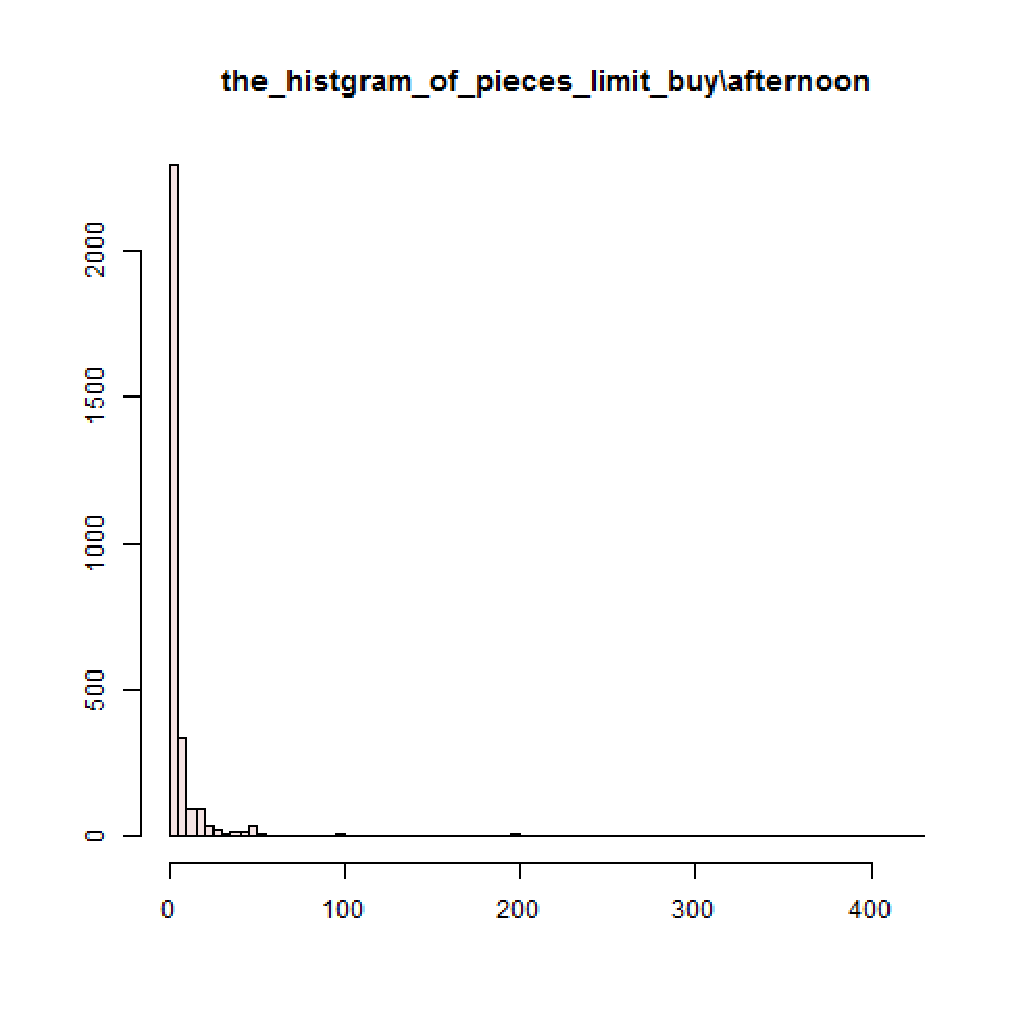
\includegraphics[clip,width = 5.0cm]{graphics/pieces_limit_buy20070129_.eps}
            \end{center}
            \caption{\scriptsize 買い指値注文の一回の注文枚数の頻度分布(2007年1月29日後場)}
        \end{minipage}
        \begin{minipage}{1\hsize}
        	\begin{center}
    			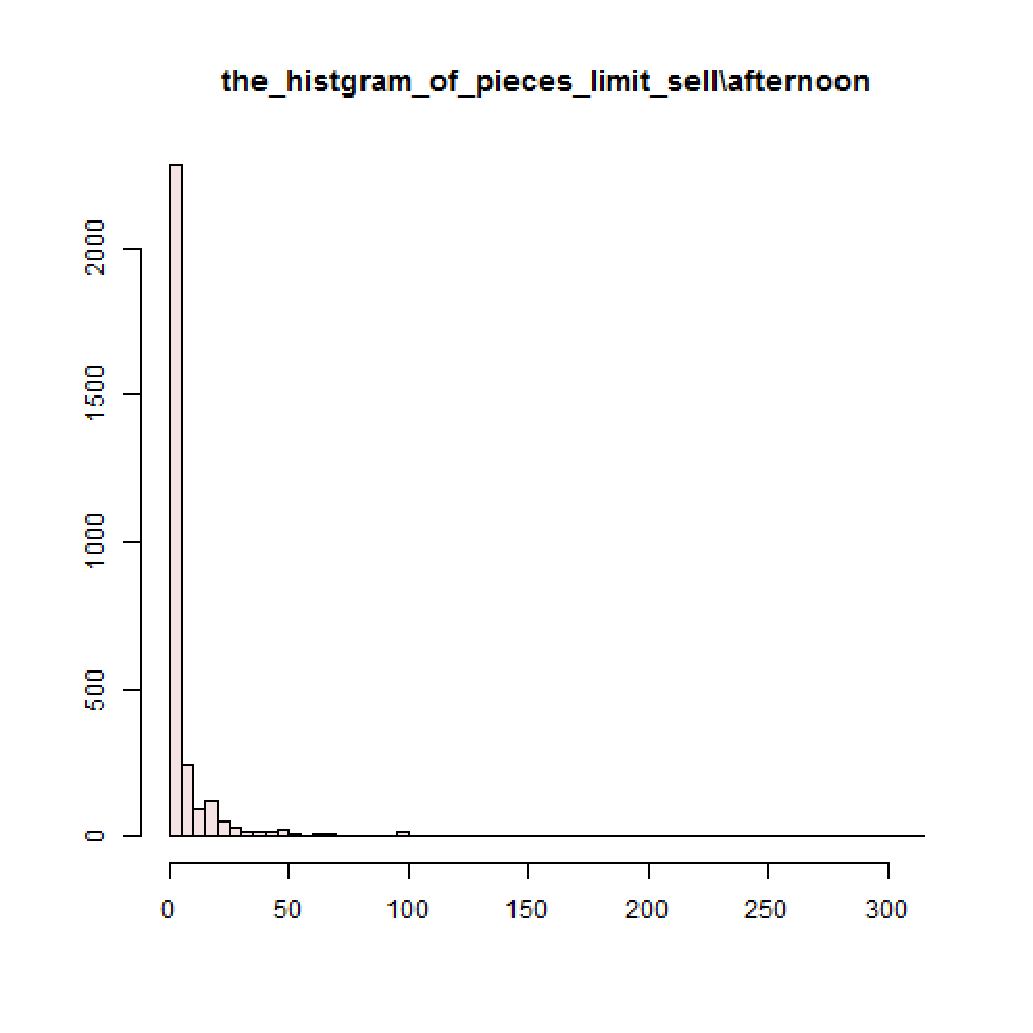
\includegraphics[clip,width = 5.0cm]{graphics/pieces_limit_sell20070129_.eps}
            \end{center}
            \caption{\scriptsize 売り指値注文の一回の注文枚数の頻度分布(2007年1月29日後場)}
        \end{minipage}
    \end{figure}
    \begin{figure}[H]
        \begin{minipage}{1\hsize}
        	\begin{center}
    			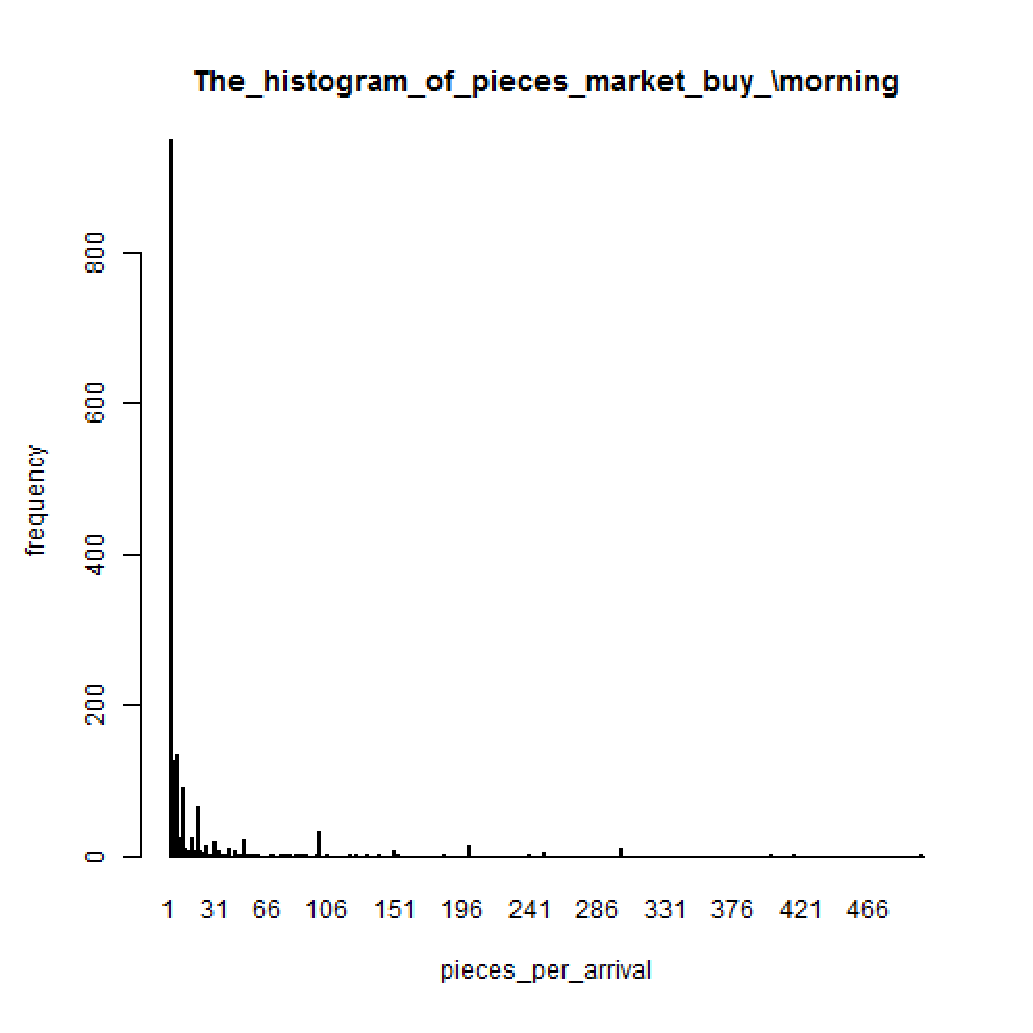
\includegraphics[clip,width = 5.0cm]{graphics/pieces_market_buy20070129_.eps}
            \end{center}
            \caption{\scriptsize 買い成行注文の一回の注文枚数の頻度分布(2007年1月29日後場)}
        \end{minipage}
        \begin{minipage}{1\hsize}
        	\begin{center}
    			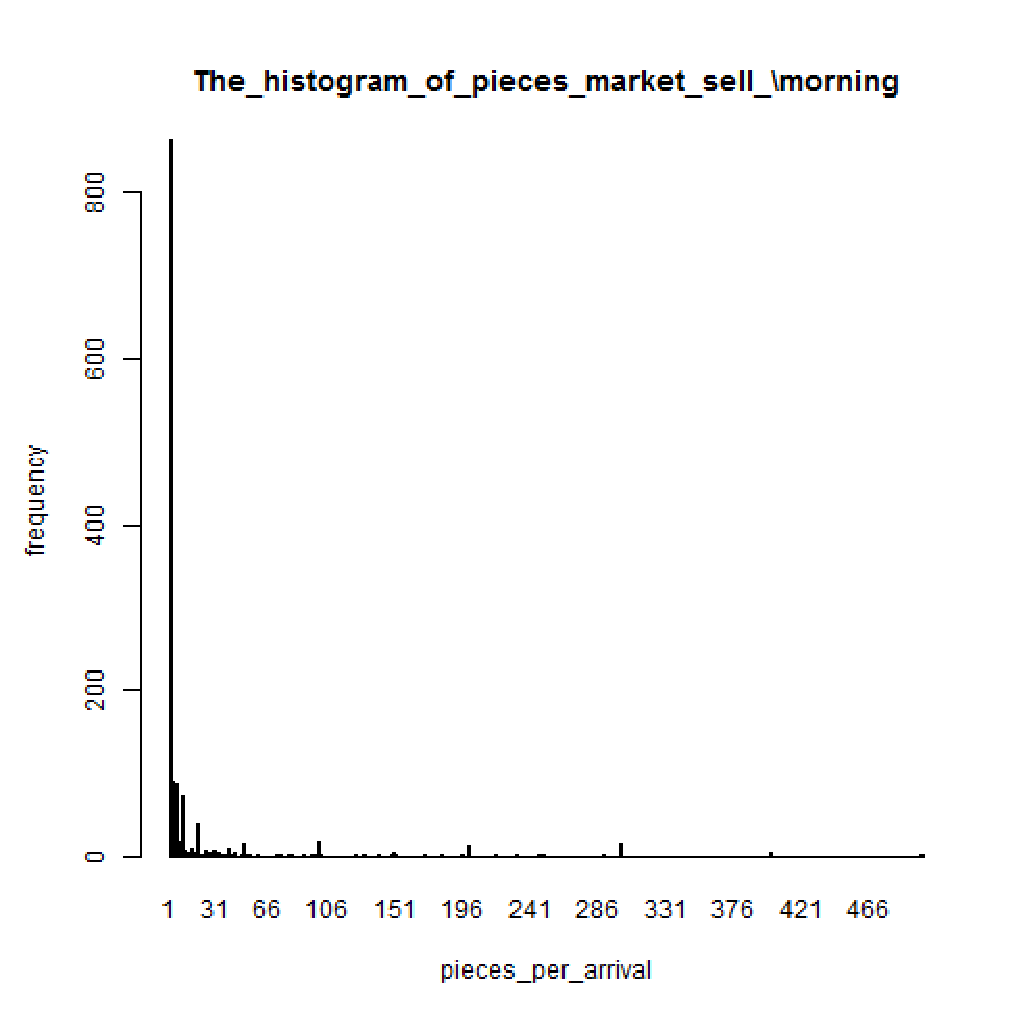
\includegraphics[clip,width = 5.0cm]{graphics/pieces_market_sell20070129_.eps}
            \end{center}
            \caption{\scriptsize 売り成行注文の一回の注文枚数の頻度分布(2007年1月29日後場)}
        \end{minipage}
    \end{figure}
    
    %到着数の統計量
    到着は小さい数字への偏りがかなり大きい.キリの良い数字($1,2,5,10,15,20,25,30,50,100,\cdots$)の注文枚数が多くなる傾向が見られる.
    
    ひとまずは一回の指値/成行の注文数は平均株数を一単位と考える(\cite{endo_zuo_kishimoto}と\cite{li_hui_endo_kishimoto}に倣う).板の解析は初期値(上下最良気配板の移動直後の板の厚み)から
    上下どちらかの板の厚みが$0$になるまでの厚みの変動を一つの待ち行列と見做し,板の移動毎にシステムが入れ替わると考える(前章までの理論部分では系内客数が$0$になってからも同一
    システム内の待ち行列を考えていた.注文時間間隔については架空サービスに対応する架空の注文を考える必要はない.).従って,注文の時間間隔を実データから抽出する際に注意するべきは,
    板の移動直前の最終の変化から板の移動が起こるまでの時間の扱いである.\\
    
    例えば最良買い気配について,板の動きの発生原因として考えられるのは次の四種類である.
    \begin{description}
    	\item[(1)] 最良買い気配数量が約定後に$0$になった場合
        \item[(2)] 最良売り気配数量が約定後に買い気配の方に飛び出した場合
    	\item[(3)] 最良気配板の幅が$2$ティック以上離れている下で,$1$ティック上に買い指値注文が来た場合
        \item[(4)] 注文がキャンセルされた場合
    \end{description}
    
    %板の移動の3パターン図
    
    抽出するべき時間間隔をまとめておく.
    \begin{table}[H]
    	\centering
    	\caption{抽出する指値/成行注文時間間隔}
        \begin{tabularx}{\linewidth}{l|X} \bhline{1.5pt}
    		観測開始点 & 板の移動直後の時間 \\ \hline \hline
        	最良気配値が変化するまで & 指値注文時間間隔,成行注文時間間隔$^\dagger$を抽出 \\ \hline \hline
        	最良買い気配値が下に移動した場合 & 移動直前に売りの成行注文があれば,その直近の売り成行注文から移動するまでの時間間隔を抽出 \\ \hline
        	最良売り気配値が上に移動した場合 & 移動直前に買いの成行注文があれば,その直近の買い成行注文から移動するまでの時間間隔を抽出 \\ \bhline{1.5pt}
        \end{tabularx}
        ({\footnotesize $\dagger$ 最良気配値にかかる数量が増加したら指値注文と判定する.減少したら,直前に約定があった場合のみ成行注文と判定する.})
    \end{table}
    
    この表に従って注文時間間隔を抽出する.
    
    また本研究では最良気配板の幅は常に$1$ティックであると仮定する.この仮定の妥当性のために$2$ティック以上離れている場合の時間が実際にどの程度なものであるかを示しておく.\\
    \begin{table}[H]
    	\centering
        \caption{最良気配値が$2$ティック以上離れている時間の割合(ザラバ時間全体を$1^\dagger$)}
        \small
        \begin{tabularx}{\linewidth}{l|lllll} \bhline{1.5pt}
        	 & {\rm Mean} & {\rm S.D.} & {\rm Median} & {\rm Minimum} & {\rm Maximum} \\ \hline
			$2006$ & $0.0195060586120777$ & $0.0677030612181418$ & $0.00208333333333333$ & $0$ & $0.444677871148459$ \\ \hline
			$2007$ & $0.0178285424121045$ & $0.0581349570904776$ & $0.00152777777777778$ & $0$ & $0.4403125$ \\ \hline
			$2008$ & $0.0332312105329688$ & $0.0880252112366147$ & $0.00168067226890756$ & $0$ & $0.502638888888889$ \\ \hline
			$2009$ & $0.0223041411093031$ & $0.0745940247185671$ & $0.000280112044817927$ & $0$ & $0.528645833333334$ \\ \hline
			$2010$ & $0.012512868645862$ & $0.0441851698948499$ & $0.000104166666666667$ & $0$ & $0.271666666666667$ \\ \hline
			$2011$ & $0.0091210487702376$ & $0.0348545571469177$ & $0.000135183850310542$ & $0$ & $0.293335736493489$ \\ \hline
			$2012$ & $0.0122896789716011$ & $0.0416945442875364$ & $0.000405441931705559$ & $0$ & $0.276624548736462$ \\ \hline
			$2013$ & $0.0185712489739548$ & $0.0612671979011189$ & $0.0018696636297624$ & $0$ & $0.51998377866895$ \\ \hline
			$2014$ & $0.0166132007108484$ & $0.0476355178792572$ & $0.000630687449319758$ & $0$ & $0.291937522571325$ \\ \hline
			$2015$ & $0.0213608996150105$ & $0.0656884482873762$ & $0.000180220770443794$ & $0$ & $0.385774209553012$ \\ \hline
			$2016$ & $0.0189805096200252$ & $0.0121494739702889$ & $0.0174577108570219$ & $0$ & $0.071640984049742$ \\ \bhline{1.5pt}
        \end{tabularx}
        ($\dagger$ 前場後場に分かれている日は前場後場それぞれのザラバの時間を$1$としている.)
    \end{table}

    
    $M/M/1$では到着時間間隔とサービス時間間隔が指数分布に従っていると仮定していた.注文時間間隔についてその仮定が妥当であるかどうかを調べる必要がある.
    分布の検定は$\chi^2$乗適合度検定による.検定の理論について%を参照されたい.\\
    帰無仮説は"実データの時間間隔が仮定する分布に従っていること"であり,棄却の有意水準は$5\%$とする.
    \begin{table}[H]
    	\centering
        \caption{検定の手順(有意水準$\alpha\ (0 < \alpha < 1)$)}
        \begin{tabularx}{\linewidth}{l|X} \bhline{1.5pt}
        	手順1 & 従っていると仮定する分布のパラメータの最尤推定量を計算する.\\ \hline
            手順2 & 時間間隔の区間を$[0, 1),[1, 2),[2, 3),\cdots,[9, 10),[10. \infty)$とし,実データの各時間間隔の頻度を計算する.\\ \hline
            手順3 & 最尤推定量をパラメータとする分布で各時間区間の確率を計算し,総データ数を掛けて頻度の理論値とする.\\ \hline
            手順4 & 各時間区間で\ $(\mbox{実現頻度-理論頻度})^2 / \mbox{理論頻度}$\ を計算,その総和が $\chi^2$ 検定等計量である.時間を$11$分割しているので,
            $2$を引いた数$9$が検定の自由度であり,その自由度の $\chi^2$ 分布の$(1-\alpha)$の確率点が検定統計量以下であれば帰無仮説を棄却する.\\ \bhline{1.5pt}
        \end{tabularx}
    \end{table}
            
    指数分布に従っていると仮定した下でのパラメータ$\lambda$と$\mu$の最尤推定量は,それぞれ$\ 1/\mbox{平均到着時間間隔}\ $,$1/\mbox{平均サービス時間間隔}\ $である.
    平均到着時間と平均サービス時間は各日の前場後場で別に計算し,分布の適合度の検定を各日の前場後場で別に行う.\\

\begin{comment}
\subsection{板の移動直後の最良気配の厚み}
	前節で述べた通り,板の移動毎にシステムが入れ替わると考える.これはどういうことか,板が移動するごとにシステムは新規の初期状態から始まるということある.
    この初期状態が板の移動直後の最良気配の厚みである.下図は板の移動直後の厚みの分布である.最良気配値の幅は常に$1$ティックと仮定して考えるから,
    ヒストグラム作成に用いた初期状態のデータはすべて最良気配値の幅は常に$1$ティックである時点のものである.
    %板の移動直後の絵
    
    板の移動直後の厚みの頻度分布を掲示しておく.
    
    ひとまずは,\cite{li_hui_endo_kishimoto}に倣ってこの初期状態はその平均値のみを取るものと考えておく.
\end{comment}

\subsection{モデルの変数と式}
	
	遠藤\cite{endo_zuo_kishimoto}と李\cite{li_hui_endo_kishimoto}に倣ってモデルで使う変数を定義する.変数につける添え字$A$と$B$はそれぞれ$ask$と$bid$の意味である.
    待ち行列理論の結果により,状態$i \geq 1$を初期状態とする$M/M/1$のシステムで系内客数が$0$になるまでの時間の分布の
    {\rm Radon-Nikodym}の意味での密度関数は以下の式で表せる.
    \begin{screen}
    	\begin{align}
    		r_i(t) &=
        	\begin{cases}	
        		\frac{i}{t} \exp{-(\lambda + \mu)t} \rho^{\frac{-i}{2}} I_{i}(2t\sqrt{\lambda \mu}) & (t > 0) \\
            	0 & (t \leq 0)
        	\end{cases} \quad (\rho = \lambda/\mu)\\
            &\mbox{$\lambda > 0:$\ 到着率,$\mu > 0:$\ サービス率,$i \geq 1:$\ 初期状態,$I_{k}(x):$\ 第一種変形{\rm Bessel}関数(定義は式(\refeq{eq:bessel_modified_bessel})).}
    	\end{align}
    \end{screen}
    ここで変数の定義を以下の通りとする:
    \begin{table}[H]
    \label{tb:def_parameters}
    	\centering
    	\caption{モデルで扱う変数の定義}
        \begin{tabular}{l|l} \bhline{1.5pt}
        	変数名 & 定義 \\ \hline \hline
    		$r_A$ & 最良売り気配数量の初期状態(板の移動直後の数量) \\ \hline
            $r_B$ & 最良買い気配数量の初期状態(板の移動直後の数量) \\ \hline
            $\lambda_A$ & 売り指値注文の到着率(1秒あたり注文数) \\ \hline
            $\lambda_B$ & 買い指値注文の到着率(1秒あたり注文数) \\ \hline
            $\mu_A$ & 買い成行注文の到着率(1秒あたりの注文数とキャンセル数の和\footnotemark) \\ \hline
            $\mu_B$ & 売り成行注文の到着率(1秒あたりの注文数とキャンセル数の和) \\ \hline
            $\rho_A$ & $\lambda_A / \mu_A$ \\ \hline
            $\rho_B$ & $\lambda_B / \mu_B$ \\ \hline
            $T_A$ & 最良売り気配数量が消滅するまでの時間 \\ \hline
            $T_B$ & 最良買い気配数量が消滅するまでの時間 \\ \hline
            $T_U$ & 最良買い気配板が消滅する前に最良売り気配の板が消滅する時間\\ \hline
            $T_D$ & 最良売り気配板が消滅する前に最良買い気配の板が消滅する時間\\ \hline
            $T_M$ & 最良買い気配板か最良売り気配のどちらかの板が消滅する時間\\ \bhline{1.5pt}
        \end{tabular}
    \end{table}
    \footnotetext{板の厚みを減らすのは成行注文だけでなく,指値注文のキャンセルも重要な因子となる.モデルの仮定では注文もキャンセルもそれぞれ或るパラメータの
    {\rm Poisson}到着をしてどの到着も独立であると仮定している.この下でなら,キャンセルを成行注文の中に含めても{\rm Poisson}分布の再生性により
    成行注文が{\rm Poisson}到着すると考えることは妥当である.}
    
\underline{\large 上下板の消滅時間の分布}\\
    上記の変数を用いて最良気配の板が消滅するまでの時間の分布の密度関数を表記する.
    \begin{align}
    	f_A(t) &\equiv 
        \begin{cases}
        		\frac{r_A}{t} \exp{-(\lambda_A + \mu_A)t} {\rho_A}^{\frac{-r_A}{2}} I_{r_A}(2t\sqrt{\lambda_A \mu_A}) & (t > 0) \\
            	0 & (t \leq 0)
        \end{cases},\\
        f_B(t) &\equiv 
        \begin{cases}
        		\frac{r_B}{t} \exp{-(\lambda_B + \mu_B)t} {\rho_B}^{\frac{-r_B}{2}} I_{r_B}(2t\sqrt{\lambda_B \mu_B}) & (t > 0) \\
            	0 & (t \leq 0)
        \end{cases}.
    \end{align}
    
    密度関数を用いて,板の消滅が有限時間内に発生する確率$\prob{T < \infty}$と消滅までの平均時間を次のように表すことができる.これらは
    指値と成行の注文の到着率の比$(\lambda/\mu)$によって場合分けされる.
    \begin{align}
    	P_A \equiv \prob{T_A < \infty} &= \int_{0}^{\infty} f_A(t) dt =
        \begin{cases}
        	1. & \rho_A \leq 1  \\
            \rho_A^{-r_A}. & \rho_A > 1
        \end{cases} \\
        P_B \equiv \prob{T_B < \infty} &= \int_{0}^{\infty} f_B(t) dt =
        \begin{cases}
        	1. & \rho_B \leq 1  \\
            \rho_B^{-r_B}. & \rho_B > 1
        \end{cases}
    \end{align}
    
    \begin{align}
    	\Exp{T_A} &= \begin{cases}
        	\frac{r_A}{\mu_A - \lambda_A}. & \rho_A < 1 \\
        	\infty. & \rho_A \geq 1
        \end{cases}\\
        \Exp{T_B} &= \begin{cases}
        	\frac{r_B}{\mu_B - \lambda_B}. & \rho_B < 1 \\
        	\infty. & \rho_B \geq 1
        \end{cases}
    \end{align}
    
\underline{\large 板が移動する時間間隔の分布}\\
    最良買い気配板が消滅する前に最良売り気配の板が消滅する(板が上に移動する)時間$T_U$の分布は
    \begin{align}
    	\prob{T_U \leq t} &= \prob{\mbox{最良売り気配板が時間$t$内に消滅する}} \\
        &\quad- \prob{\mbox{最良買い気配板が消滅した後に最良売り気配板が時間$t$内に消滅する}} \\
        &= \prob{T_A \leq t} - \prob{T_B \leq T_A \leq t} \\
        &= \int_{0}^{t} f_A(\tau)d\tau - \int_{0}^{t} f_A(\tau) \left( \int_{0}^{\tau} f_B(s)ds \right) d\tau, \quad (t>0)
    \end{align}
    と表される.最右辺を微分して$T_U$の分布の密度関数$f_U(t)$を得る(被積分関数が連続であるから微分可能).
    \begin{align}
    	f_U(t) \equiv \begin{cases}
        	f_A(t) - f_A(t) \left( \int_{0}^{t} f_B(\tau)d\tau \right), & t>0, \\
            0, & t \leq 0.
    	\end{cases}
    \end{align}
    
    同様にして最良売り気配板が消滅する前に最良買い気配の板が消滅する(板が下に移動する)時間$T_D$の分布の密度関数は
    \begin{align}
    	f_D(t) \equiv \begin{cases}
        	f_B(t) - f_B(t)\left( \int_{0}^{t}f_A(\tau)d\tau \right), & t>0, \\
            0, & t \leq 0,
        \end{cases}
    \end{align}
    と表される.有限時間内に板が上に動く確率$P_U$,下に動く確率$P_D$,変動(上に動く事象と下に動く事象の和事象)が起こる確率$P_M$は次のように表現される.
    \begin{align}
    	P_U \equiv \prob{T_U < \infty} &= \int_{0}^{\infty} f_U(t) dt \\
        &= \int_{0}^{\infty} f_A(t)dt - \int_{0}^{\infty} f_A(t) \left( \int_{0}^{t} f_B(\tau)d\tau \right) dt \\
        &= P_A - \int_{0}^{\infty} f_A(t) \left( \int_{0}^{t} f_B(\tau)d\tau \right) dt, \\
        P_D \equiv \prob{T_D < \infty} &= \int_{0}^{\infty} f_D(t) dt \\
        &= \int_{0}^{\infty} f_B(t)dt - \int_{0}^{\infty} f_B(t) \left( \int_{0}^{t} f_A(\tau)d\tau \right) dt \\
        &= P_B - \int_{0}^{\infty} f_B(t) \left( \int_{0}^{t} f_A(\tau)d\tau \right) dt. \\
    \end{align}
    ここで最終式の第二項について,被積分関数が非負で可積分であるから{\rm Fubini}の定理の適用で積分の順序交換が正当化される:
    \begin{align}
    	\int_{0}^{\infty} f_B(t) \left( \int_{0}^{t} f_A(\tau)d\tau \right) dt = \int_{0}^{\infty} f_A(t) \left( \int_{t}^{\infty} f_B(\tau)d\tau \right) dt
    \end{align}
    この変形式を元の式に代入することで,$P_M$は次の表現になる.
    \begin{align}
    	P_M = \prob{T_M < \infty} &\equiv P_U + P_D \\
        &= P_A - \int_{0}^{\infty} f_A(t) \left( \int_{0}^{t} f_B(\tau)d\tau \right) dt + 
        	P_B - \int_{0}^{\infty} f_A(t) \left( \int_{t}^{\infty} f_B(\tau)d\tau \right) dt \\
        &= P_A + P_B - \int_{0}^{\infty} f_A(t) \left( \int_{0}^{\infty} f_B(\tau)d\tau \right) dt \\
        &= P_A + P_B - P_A P_B \\
        &= \begin{cases}
        	1, & \rho_A \leq 1\ or\ \rho_B \leq 1, \\
            \alpha(< 1), & \rho_A > 1\ and\ \rho_B > 1.
        \end{cases}
    \end{align}
    
    変動が起こるまでの時間$T_M$の平均値は次のように表せる.
    \begin{align}
    	\int_{0}^{\infty} t d\prob{T_M \leq t} &= \int_{0}^{\infty} t d(\prob{T_U \leq t} + \prob{T_D \leq t}) \\
        &= \int_{0}^{\infty} t f_U(t) dt + \int_{0}^{\infty} t f_D(t) dt.
    \end{align}
    
\underline{\large 転移行列}\\
    「板が上昇する」「板が下降する」を二種類の状態と見做して,直前に上昇し続けて上昇する確率$p_{UU}$,直前に上昇し次に下降する確率$p_{UD}$,
    直前に下降し続けて下降する確率$p_{DD}$,直前に下降し次に上昇する確率$p_{DU}$の四つの転移確率を定義する.注文の時間間隔が独立に指数分布に従っていると仮定している
    下で,その無記憶性からこの状態推移は一次の{\rm Marcov}過程と考えることができる.転移行列$P$は次のように表せる.
    \begin{align}
    	P \equiv \left(
    	\begin{array}{@{\,}cc@{\,}}
    		p_{UU} & p_{UD} \\
            p_{DU} & p_{DD}
    	\end{array}
    	\right). \\ \label{eq:transient_probability_matrix}
    \end{align}
    $f_A(t)(f_B(t))$は$r_A(r_B)$に,$f_U(t)$と$f_D(t)$は$r_A$と$r_B$の両方に依存する関数であったから,これらを
    $f_A(t \mid r_A), f_B(t \mid r_B), f_U(t \mid r_A, r_B), f_D(t \mid r_A, r_B)$と表記し直す.ここで,板が上昇した直後の
    上下板の初期状態をそれぞれ$r_A^U, r_B^U$,板が下降した直後の上下板の初期状態をそれぞれ$r_A^D, r_B^D$と表記すると,
    先の転移確率は次の式で表せる.
    \begin{align}
    	p_{UU} &= \int_{0}^{\infty} f_U(t \mid r_A^U, r_B^U) dt = \int_{0}^{\infty} f_A(t \mid r_A^U)dt - \int_{0}^{\infty} f_A(t \mid r_A^U) \left( \int_{0}^{t} f_B(\tau \mid r_B^U)d\tau \right) dt, \\
        p_{UD} &= \int_{0}^{\infty} f_D(t \mid r_A^U, r_B^U) dt = \int_{0}^{\infty} f_B(t \mid r_B^U)dt - \int_{0}^{\infty} f_B(t \mid r_B^U) \left( \int_{0}^{t} f_A(\tau \mid r_A^U)d\tau \right) dt, \\
        p_{DU} &= \int_{0}^{\infty} f_U(t \mid r_A^D, r_B^D) dt = \int_{0}^{\infty} f_A(t \mid r_A^D)dt - \int_{0}^{\infty} f_A(t \mid r_A^D) \left( \int_{0}^{t} f_B(\tau \mid r_B^D)d\tau \right) dt, \\
        p_{DD} &= \int_{0}^{\infty} f_D(t \mid r_A^D, r_B^D) dt = \int_{0}^{\infty} f_B(t \mid r_B^D)dt - \int_{0}^{\infty} f_B(t \mid r_B^D) \left( \int_{0}^{t} f_A(\tau \mid r_A^D)d\tau \right) dt.
    \end{align}
    先の転移行列を有つ{\rm Marcov}過程の定常分布を計算しておく.考えている状態は「上昇する」と「下降する」の二種類であるから,
    上昇する確率を$p_U$,下降する確率を$p_D$と表記しておく.この分布$\pi \equiv (p_U,\ p_D)$が定常となる場合を考える.
    定常分布と転移行列$P$を用いて次の関係(平衡方程式)が成り立つ.
    \begin{align}
    	\pi P = \pi.
    \end{align}
    この式を満たすような分布$\pi$を求める.これは行列$P$についての固有値問題を解くことにもなると示しておく.表記の便宜を図って
    \begin{align}
    	(x,y) \left(
    	\begin{array}{@{\,}cc@{\,}}
    		a & 1-a \\
            1-b & b
    	\end{array}
    	\right)
        = \lambda(x,y), \quad (0 \leq a, b, x, y \leq 1,\ x+y=1), \label{eq:balance_equation}
    \end{align}
    を解く.固有方程式は
    \begin{align}
    	\lambda^2 - (a + b)\lambda + ab - (1-a)(1-b)
        &= \lambda^2 - (a + b)\lambda + a + b - 1 \\
        &= (\lambda - 1)(\lambda - a - b + 1) \\
        &= 0,
    \end{align}
    であるから,定常分布の計算は式(\refeq{eq:balance_equation})にて行列の固有値$1$の固有ベクトルを計算することと同じである.
    連立方程式を解けば結果は$(1-a)x=(1-b)y$であると判り,$a,b$を$p_{UU}, p_{DD}$で置き換えれば次の結果を得る.
    \begin{align}
    	p_U &= \frac{1-p_{DD}}{1 - p_{UU} + 1 - p_{DD}} = \frac{p_{DU}}{p_{UD}+p_{DU}}, \\
        p_D &= \frac{1-p_{UU}}{1 - p_{UU} + 1 - p_{DD}} = \frac{p_{UD}}{p_{UD}+p_{DU}}. \label{eq:stationary_dist}
    \end{align}
    
\underline{\large 確率的初期状態}\\
    板の初期状態が或る分布に従っていると考える.板の初期状態がその分布に従う確率変数$R_A, R_B$で与えられ両者の分布が独立である場合に,上下板それぞれについて先に消滅する
    時間の密度関数$f_U^R,f_D^R$は先の$f_U(t \mid r_A, r_B), f_D(t \mid r_A, r_B)$を用いて次のように表現できる.
    \begin{align}
    	f_U^R (t) \equiv \int_{0}^{\infty}\!\!\!\int_{1}^{\infty} f_U(t \mid r_A, r_B) d\prob{R_A = r_A}d\prob{R_B = r_B}, \\
        f_D^R (t) \equiv \int_{0}^{\infty}\!\!\!\int_{1}^{\infty} f_D(t \mid r_A, r_B) d\prob{R_A = r_A}d\prob{R_B = r_B}.
    \end{align}
    これも{\rm Fubini}の定理による.
    \begin{align}
    	\prob{T_U \leq t} &= \int_{0}^{\infty}\!\!\!\int_{0}^{\infty} \left( \int_{0}^{t} f_U(\tau \mid r_A, r_B) d\tau \right) d\prob{R_A = r_A}d\prob{R_B = r_B} \\
        &= \int_{0}^{t} \left( \int_{0}^{\infty}\!\!\!\int_{0}^{\infty} f_U(\tau \mid r_A, r_B) d\prob{R_A = r_A}d\prob{R_B = r_B} \right) d\tau, \\
    	\Rightarrow f_U^R (t) &= \int_{0}^{\infty}\!\!\!\int_{0}^{\infty} f_U(t \mid r_A, r_B) d\prob{R_A = r_A}d\prob{R_B = r_B}. \hfill \qed
    \end{align}

\subsection{抽出データ}
    実際のデータから取り出した,指値/成行注文の頻度,一回の注文枚数,最良気配値の上昇/下降回数を表にしたものを掲示する.
    注文の頻度と板の上下変動回数については,各日の前場後場毎に数えられたものから平均,標準偏差などを計算している.
    \begin{table}[H]
    	\centering
        \caption{指値/成行注文の頻度, 一回の注文枚数, 最良気配値の上昇/下降回数\ ($2007$年)}
        \fontsize{6pt}\selectfont
    	\begin{tabularx}{\linewidth}{l||lllllll} \bhline{1.5pt}
        \label{tb:statistics_parameters}
        	  & {\rm Mean} & {\rm S.D.} & {\rm Median} & {\rm Kurtosis} & {\rm Skewness} & {\rm Minimum} & {\rm Maximum} \\ \hline
			{\rm Arrival Frequency of Market Buy Orders} & $1874.5512295082$ & $907.457993347613$ & $1820.5$ & $5.11767451501856$ & $0.675337509991397$ & $71$ & $6360$ \\ \hline
			{\rm Arrival Frequency of Market sell Orders} & $1885.09221311475$ & $953.983272328056$ & $1821$ & $6.79006081829123$ & $0.984428247560377$ & $71$ & $8120$ \\ \hline
			{\rm Arrival Frequency of canceled Buy Orders} & $1665.64344262295$ & $548.418678697007$ & $1591.5$ & $4.34069326524823$ & $1.0223638226889$ & $664$ & $3738$ \\ \hline
			{\rm Arrival Frequency of canceled sell Orders} & $1619.41803278689$ & $547.114909569955$ & $1536.5$ & $4.37945019113223$ & $1.02533665819909$ & $579$ & $3781$ \\ \hline
			{\rm Arrival Frequency of limit Buy Orders} & $3653.97336065574$ & $1181.78855390768$ & $3652$ & $4.05675797950432$ & $0.270126754158371$ & $732$ & $8157$ \\ \hline
			{\rm Arrival Frequency of limit sell Orders} & $3563.19057377049$ & $1145.30183541394$ & $3508$ & $4.68143888199017$ & $0.408568143055593$ & $620$ & $9012$ \\ \hline
			{\rm Averege Pieces of One Market Buy Order} & $12.5206451488378$ & $2.77323438747951$ & $12.4681411546065$ & $3.09574522739222$ & $-0.251787164006476$ & $3.56578947368421$ & $19.3492990654206$ \\ \hline
			{\rm Averege Pieces of One Market sell Order} & $12.4193657939448$ & $2.9010116850716$ & $12.4853634546859$ & $3.03603809159898$ & $-0.467023405948823$ & $3.66887417218543$ & $18.7199881726789$ \\ \hline
			{\rm Averege Pieces of One canceled Buy Order} & $9.67245218614441$ & $2.00315704051638$ & $9.37503694441844$ & $5.71568254649852$ & $1.32236478548353$ & $5.98338870431894$ & $19.3528114663727$ \\ \hline
			{\rm Averege Pieces of One canceled sell Order} & $9.81634156546921$ & $2.22155817463813$ & $9.34956284664529$ & $5.43345907724932$ & $1.3486729418014$ & $4.8828903654485$ & $19.7518610421836$ \\ \hline
			{\rm Averege Pieces of One limit Buy Order} & $9.14417038292241$ & $1.68568811350152$ & $8.89759617833488$ & $4.28773924054411$ & $0.915406332348662$ & $5.73312765136907$ & $15.9323899371069$ \\ \hline
			{\rm Averege Pieces of One limit sell Order} & $9.40128432350844$ & $1.90029143582777$ & $9.10787585849688$ & $3.73751115997436$ & $0.927845553013401$ & $5.66795366795367$ & $16.4413665743306$ \\ \hline
			{\rm Upmovement Times Of the Best Bid} & $120.290983606557$ & $75.1582407362664$ & $101$ & $14.0082219500023$ & $2.43447280583046$ & $17$ & $719$ \\ \hline
			{\rm Downmovement Times Of the Best Bid} & $92.8709016393443$ & $55.685698856088$ & $82$ & $20.9273670184347$ & $2.97402869075286$ & $14$ & $610$ \\ \hline
			{\rm Upmovement Times Of the Best Ask} & $93.0409836065574$ & $54.7743397619828$ & $80$ & $16.8868891795264$ & $2.67172775656591$ & $12$ & $558$ \\ \hline
			{\rm Downmovement Times Of the Best Ask} & $119.463114754098$ & $75.5175617154362$ & $99.5$ & $18.1165736972318$ & $2.71213913991385$ & $14$ & $794$ \\ \bhline{1.5pt}
        \end{tabularx}
    \end{table}
    
    上表に示したデータの抽出方法を記述する.全てデータはザラバ開始後 $\sim$ 場の引けまでの間から抽出する.これは寄付の約定が確認された直後から引けの約定が確認される
    直前までのことである.まず成行注文について,注文回数は約定の回数に等しい.約上の直後で板が上下しない場合は約定枚数を注文枚数と数える.
    しかし約上の前後のデータを見ていると板にかかる累積枚数の変化量と約定枚数が一致しない場合がある.
    この場合はその増減に応じて指値注文または注文のキャンセルがあったと判断して,その回数と枚数を記録する.約定を挟んで板が上下する場合,
    成行注文枚数と約定枚数が一致するとは限らない.板にかかる枚数より多い成行注文が来れば,余りの注文枚数は上下した後の板の厚み(初期デプス)となるのである.
    余りの成行注文枚数があるかないかは板の移動直後の上下最良気配値の差額で判断する.通常上下板は$1$ティック$10$円離れているから,移動直後も
    $1$ティックの差であるなら成行注文枚数は約定枚数と余り枚数の和と見做す.約定直後で板が$2$ティック以上離れている場合,
    成行注文の余りは無かったとして約定枚数を成行注文枚数とする.約定を挟まずに板が上下する場合もある.例えば板が$2$ティック以上離れている下で
    買い板が上昇したらそれは指値注文として記録し,その他にも直前に約定がなくて買い板が下降すれば注文のキャンセルとして記録する.
    売りの場合は逆を考えれば良い.約定も板の上下も無い下での板の累積枚数の変化は,
    その増減に応じて指値注文または注文のキャンセルとして記録する.上下板の初期デプス(後述)に関しては,上下板が同時に動いたときのみを記録する.
    表\ref{tb:def_parameters}に掲載したモデル式内のパラメータについても,実際のデータから抽出したものを掲示しておく.
    \mbox{}\\
    
\underline{\large 初期デプス}\\
    板の移動直後の上下板の厚み,すなわち待ち行列の初期状態を表すパラメータについて$1$枚単位($1$枚$=1000$株)で表示する.データは
    最良気配値が$1$ティック離れている箇所のみを抽出した.これはモデルが上下の最良気配値の差額を常に$10$円と仮定しているためである.
    \begin{table}[H]
    	\centering
        \caption{最良気配の移動直後の最良気配の厚み(枚)\ ($2007$年)}
    	\begin{tabularx}{\linewidth}{l||llll} \bhline{1.5pt}
        	{\rm Initial Depth} & {\rm Best Ask (After Up)} & {\rm Best Bid (After Up)} & {\rm Best Ask (After Down)} & {\rm Best Bid (After Down)} \\ \hline \hline
            {\rm Mean} & $420.484997$ & $40.29340868$ & $40.31588898$ & $421.7710303$ \\ \hline
            {\rm S.D.} & $218.9372442$ & $63.17343688$ & $63.39659637$ & $211.8249755$ \\ \bhline{1.5pt}
        \end{tabularx}
    \end{table}
    
    板の移動直後の厚みの頻度図を見ると,これは或る確率分布に従っていると推測される.{\rm Gamma}分布に従っていると仮定した下で,
    最尤法により推定したパラメータで計算される密度関数と実際の観測された分布を下図に表す.
    \begin{align}
    	\mbox{密度関数:}f(x) = \frac{1}{\Gamma(\alpha)\beta^\alpha} x^{\alpha-1} e^{-x/\beta}, \quad(x > 0).
    \end{align}
    \begin{table}[H]
    	\centering
        \caption{{\rm Gamma}分布推定パラメータ}
        \begin{tabularx}{\linewidth}{l||lll|ll} \bhline{1.5pt}
        	{\rm } & 板上昇直後 & & & 板下降直後 & \\ \hline
        	{\rm } & \alpha & \beta & & \alpha & \beta \\ \hline \hline
			{\rm Best bid} & $0.680112458$ & $59.24521486$ & & $3.849663935$ & $109.5604804$ \\ \hline
			{\rm Best ask} & $3.805877022$ & $110.4830751$ & & $0.673427365$ & $59.86672222$ \\ \bhline{1.5pt}
        \end{tabularx}
        \label{tab:initial_depth_parameters}
    \end{table}
    
    \begin{figure}[H]
        \begin{center}
    	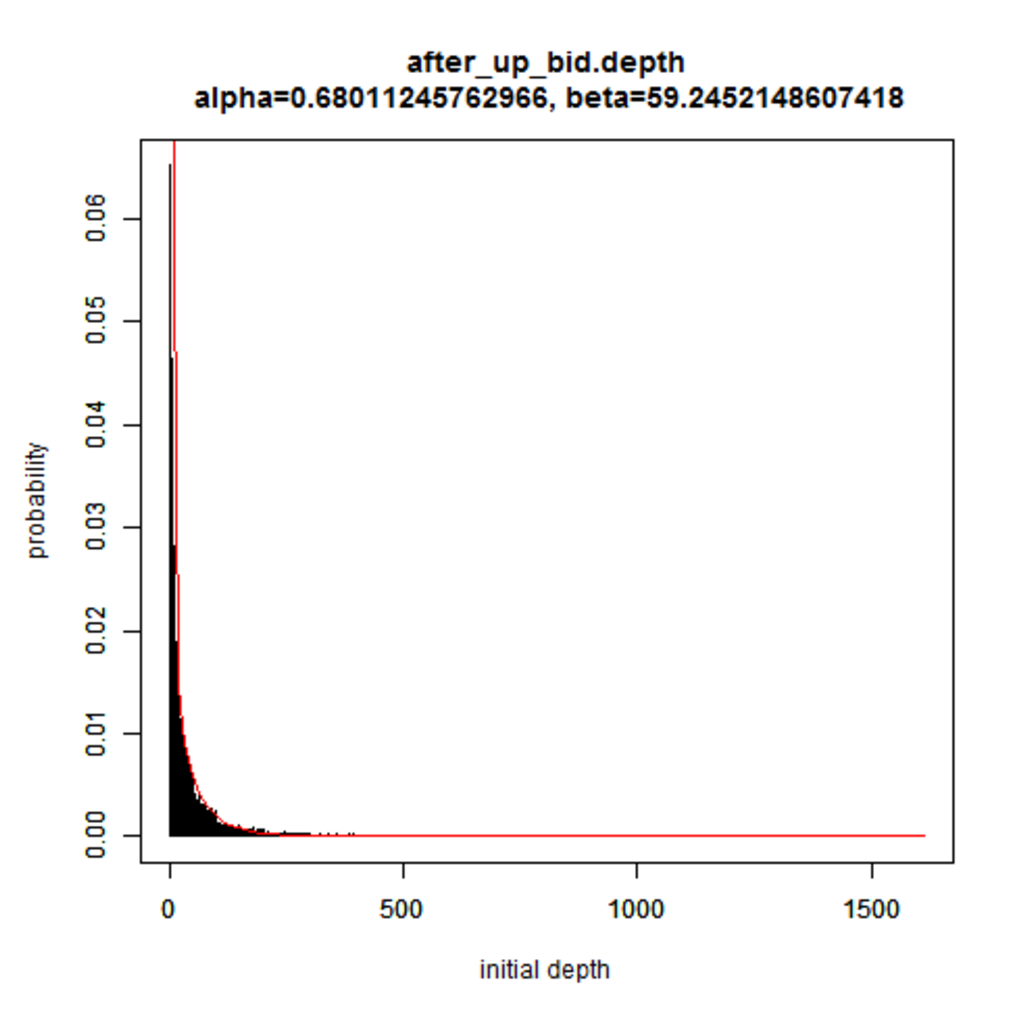
\includegraphics[clip,width = 10.0cm]{graphics/after_up_bid.depth.eps}
        \end{center}
        \caption{板上昇直後初期デプス({\rm Best bid})}
    \end{figure}
    \begin{figure}[H]
        \begin{center}
    	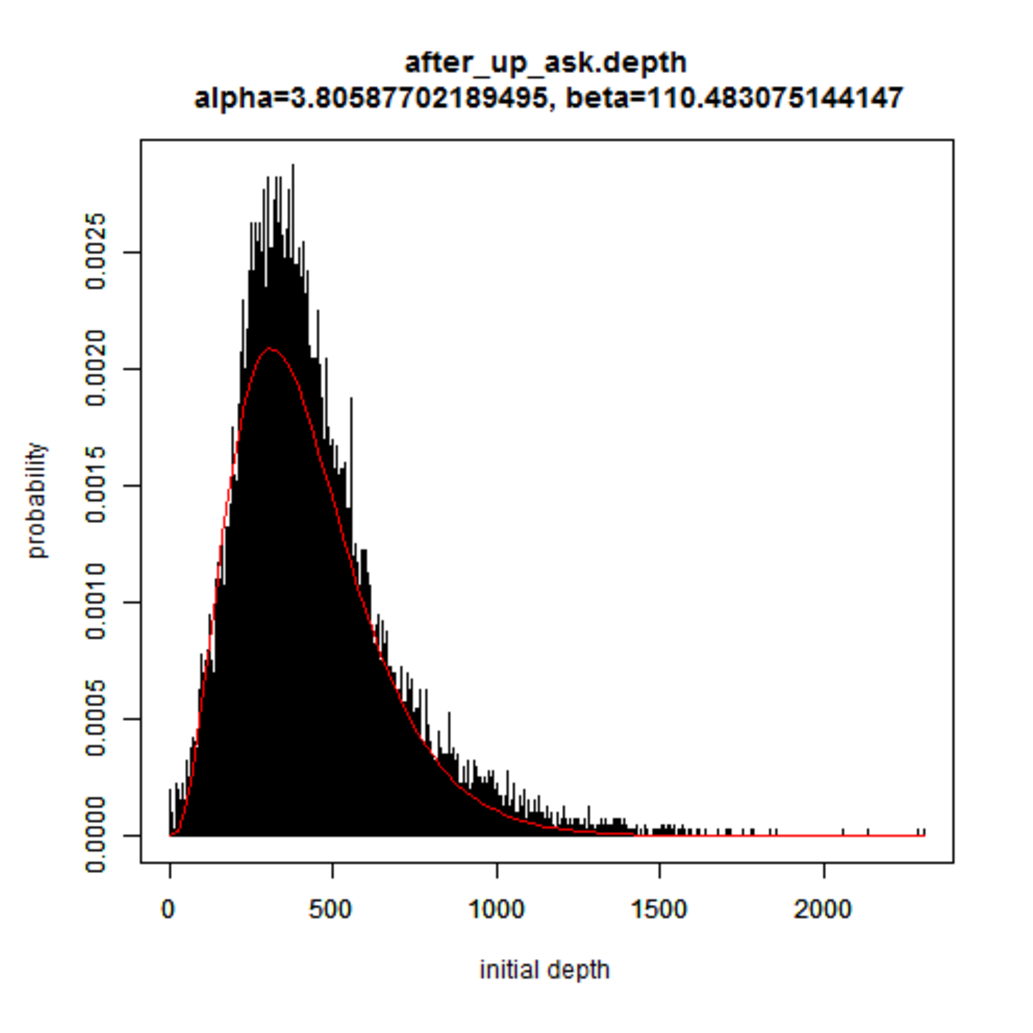
\includegraphics[clip,width = 10.0cm]{graphics/after_up_ask.depth.eps}
        \end{center}
        \caption{板上昇直後初期デプス({\rm Best ask})}
    \end{figure}
    \begin{figure}[H]
        \begin{center}
    	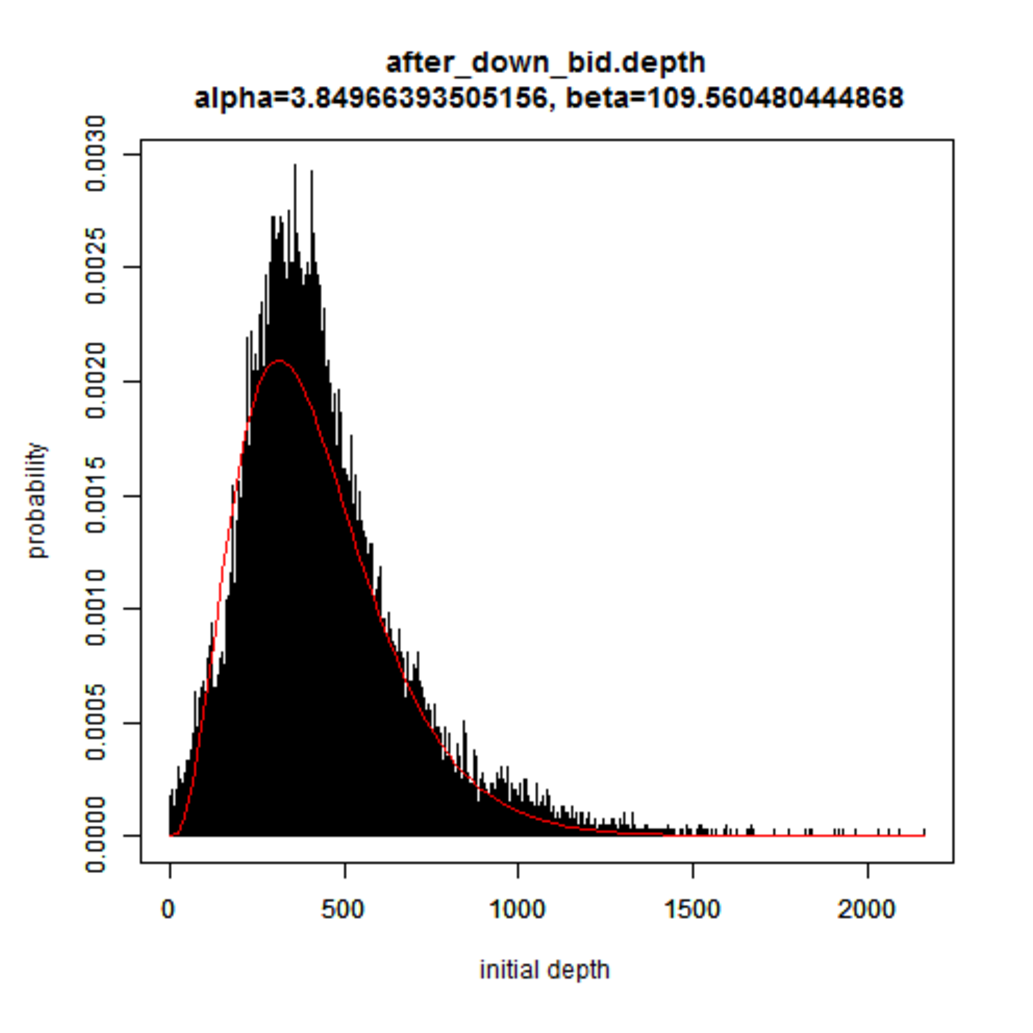
\includegraphics[clip,width = 10.0cm]{graphics/after_down_bid.depth.eps}
        \end{center}
        \caption{板下降直後初期デプス({\rm Best bid})}
    \end{figure}
    \begin{figure}[H]
        \begin{center}
    	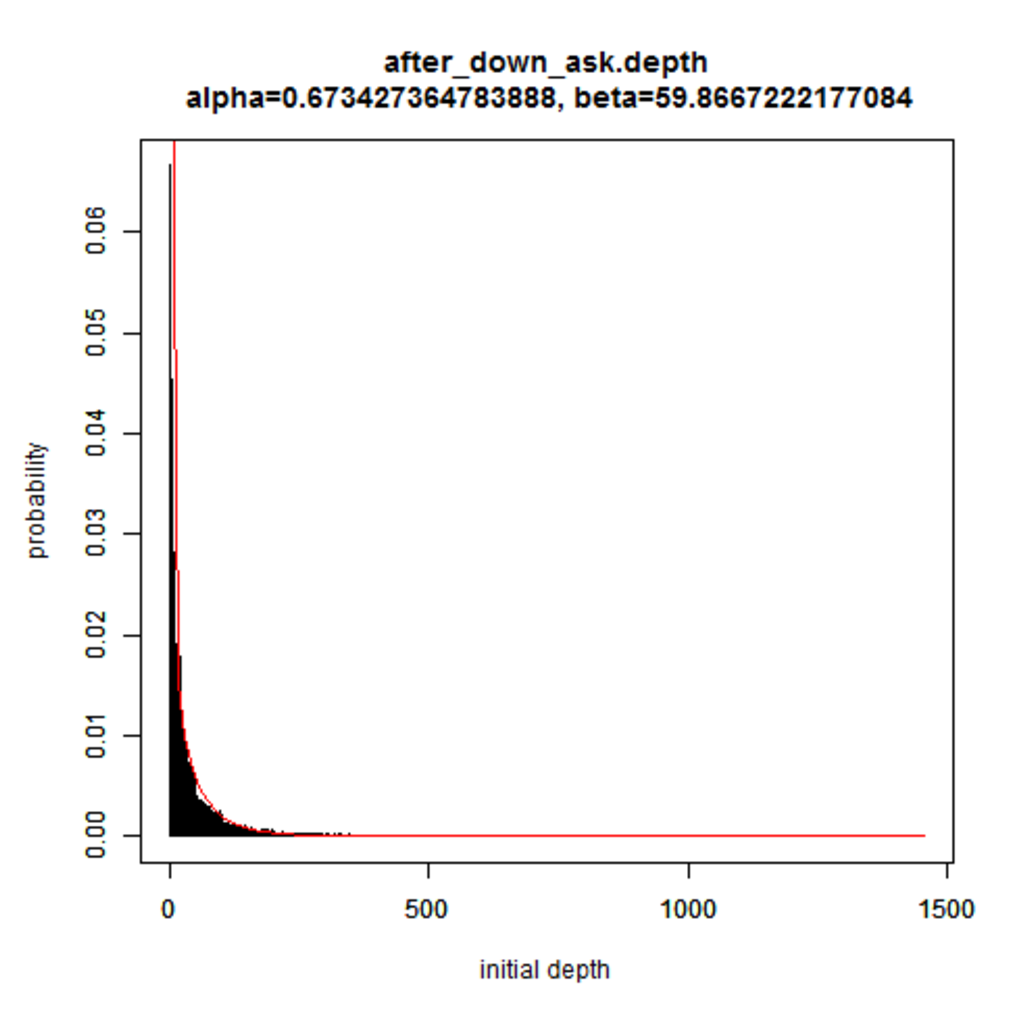
\includegraphics[clip,width = 10.0cm]{graphics/after_down_ask.depth.eps}
        \end{center}
        \caption{板下降直後初期デプス({\rm Best ask})}
    \end{figure}
    
\underline{\large 到着率}\\
	$M/M/1$の待ち行列理論では一度に複数単位到着する確率は$0$としている.実際の注文は一度に複数単位到着することが多いから,理論に合わせるために
    複数単位の到着を一単位の到着の複数回ということに読み直す必要がある.到着数の単位について,本研究においては$1$枚一単位,$10$枚一単位,
    $30$枚一単位の三つの場合を考える.到着率とは一秒あたりの到着数のことである.以下に示す到着率は,
    $(1)$単純に到着数を測ったもの,
    $(2)$毎度$1$枚ずつ到着すると見做して到着率を測ったもの($N$枚の到着は$1$枚の到着の$N$回分),
    $(3)$$10$枚累積した時点を一回の到着として到着数を測ったもの,
    $(4)$$30$枚累積した時点を一回の到着として到着数を測ったもの,の四種類を計算した.\cite{miyazaki}に倣い,注文の到着率の最尤推定量を次の式で計算する.
    \begin{align}
    	\frac{\mbox{観測時間内の到着数}}{\mbox{観測時間}}.
    \end{align}
    観測時間はザラバ全体(昼休みがある場合は午前午後で分ける)とし,時間単位は秒である.
    データの到着時間は秒単位まで切り捨てられているが,実際の到着時間は実数秒であると考える.
    \begin{table}[H]
    	\centering
        \caption{指値/成行注文の到着率 単純に到着数を測ったもの\ ($2007$年)}
    	\begin{tabularx}{\linewidth}{l||llll} \bhline{1.5pt}
        \label{arrival_rate_per_second_1}
         	{\rm Arrival Rate Per Second} & \lambda_B & \lambda_A & \mu_A & \mu_B \\ \hline
			{\rm Mean} & $0.440430079307341$ & $0.429770731607785$ & $0.42123513769926$ & $0.42834751029013$ \\ \hline
			{\rm S.D.} & $0.139350721669983$ & $0.134820939951023$ & $0.151662215771227$ & $0.160366521869234$ \\ \bhline{1.5pt}
        \end{tabularx}
    \end{table}
    
    \begin{table}[H]
    	\centering
        \caption{指値/成行注文の到着率 一回の到着は$1$枚として到着数を測ったもの\ ($2007$年)}
    	\begin{tabularx}{\linewidth}{l||llll} \bhline{1.5pt}
        \label{arrival_rate_per_second_2}
        	{\rm Arrival Rate Per Second} & \lambda_B & \lambda_A & \mu_A & \mu_B \\ \hline
			{\rm Mean} & $4.04720476425838$ & $4.03655030768043$ & $4.86637047632663$ & $4.89119891472509$ \\ \hline
			{\rm S.D.} & $1.63421331941915$ & $1.62678973960703$ & $2.06954754281546$ & $2.18770444650317$ \\ \bhline{1.5pt}
        \end{tabularx}
    \end{table}
    
    \begin{table}[H]
    	\centering
        \caption{指値/成行注文の到着率 $10$枚累積した時点を一回の到着として到着数を測ったもの\ ($2007$年)}
    	\begin{tabularx}{\linewidth}{l||llll} \bhline{1.5pt}
        \label{arrival_rate_per_second_3}
        	{\rm Arrival Rate Per Second} & \lambda_B & \lambda_A & \mu_A & \mu_B \\ \hline
			{\rm Mean} & $0.404665416528414$ & $0.403597612483072$ & $0.486585672358297$ & $0.489064243868232$ \\ \hline
			{\rm S.D.} & $0.163421290234038$ & $0.162676317541532$ & $0.206955155383898$ & $0.218769843276613$ \\ \bhline{1.5pt}
        \end{tabularx}
    \end{table}
    
    \begin{table}[H]
    	\centering
        \caption{指値/成行注文の到着率 $30$枚累積した時点を一回の到着として到着数を測ったもの\ ($2007$年)}
    	\begin{tabularx}{\linewidth}{l||llll} \bhline{1.5pt}
        \label{arrival_rate_per_second_4}
        	{\rm Arrival Rate Per Second} & \lambda_B & \lambda_A & \mu_A & \mu_B \\ \hline
			{\rm Mean} & $0.134847084292512$ & $0.134493211764554$ & $0.162157327962169$ & $0.162979523115285$ \\ \hline
			{\rm S.D.} & $0.0544755143646112$ & $0.0542254514351687$ & $0.0689828043027468$ & $0.07292086367212$ \\ \bhline{1.5pt}
        \end{tabularx}
    \end{table}

\begin{comment}
    上表の結果は\cite{li_hui_endo_kishimoto}の結果と大分違った.\cite{li_hui_endo_kishimoto}では到着率を分単位で計算していて,
    その結果は$\lambda_B=3.77, \lambda_A=3.72, \mu_A=4.71, \mu_B=4.65$である.今回の結果を$60$倍してもこの数字には近くない.
    但し,\cite{li_hui_endo_kishimoto}が基にしているデータ期間は$2006/12/11 \sim 2007/12/13$であり,
    今回のデータは$2007/01/04 \sim 2007/12/28$であるから,およそ$10$日間のズレがある.それでも計算された結果があまりにも違った.\\
    \mbox{}\\
\end{comment}
    
\underline{\large 推移確率行列}\\
	式(\refeq{eq:transient_probability_matrix})で定義される転移確率の理論値を計算する.到着率のパラメータは先述の三種類のものを使った.
    行列要素の括弧の中の数値は標準偏差を表す.
    \begin{description}
    	\item[実際に観測された推移確率]\mbox{}\\
        	上下板が同時に動いた箇所のみ勘定した結果を示しておく.
        	\begin{align}
    			\left(
    			\begin{array}{@{\,}cc@{\,}}
    				p_{UU} & p_{UD} \\
            		p_{DU} & p_{DD}
    			\end{array}
    			\right)
                = \left(
    			\begin{array}{@{\,}cc@{\,}}
    				\substack{0.323 \\ (0.298)} & \substack{0.677 \\ (0.298)} \\
            		\substack{0.682 \\ (0.284)} & \substack{0.318 \\ (0.284)}
    			\end{array}
    			\right).
    		\end{align}

        \item[$10$枚累積した時点を一回の到着として測った到着数による到着率(10枚を一単位として計算)]\mbox{}\\
        	\begin{align}
    			\left(
    			\begin{array}{@{\,}cc@{\,}}
    				p_{UU} & p_{UD} \\
            		p_{DU} & p_{DD}
    			\end{array}
    			\right)
                = \left(
    			\begin{array}{@{\,}cc@{\,}}
    				\substack{0.0567 \\ (0.0936)} & \substack{0.941 \\ (0.0929)} \\
            		\substack{0.946 \\ (0.0802)} & \substack{0.0535 \\ (0.0826)}
    			\end{array}
    			\right).
    		\end{align}
        
        \item[$30$枚累積した時点を一回の到着として測った到着数による到着率(30枚を一単位として計算)]\mbox{}\\
        	\begin{align}
    			\left(
    			\begin{array}{@{\,}cc@{\,}}
    				p_{UU} & p_{UD} \\
            		p_{DU} & p_{DD}
    			\end{array}
    			\right)
                = \left(
    			\begin{array}{@{\,}cc@{\,}}
    				\substack{0.06799 \\ (0.0655)} & \substack{0.922 \\ (0.0793)} \\
            		\substack{0.922 \\ (0.0876)} & \substack{0.0655 \\ (0.0647)}
    			\end{array}
    			\right).
    		\end{align}
    \end{description}
    
    続いて初期デプスが確率変動すると仮定した場合の転移確率を計算する.初期デプス$r_A, r_B$が表(\ref{tab:initial_depth_parameters})に示すパラメータを有つ
    {\rm Gamma}分布に従うと仮定した時,その密度関数を$g_A, g_B$と表せば,転移確率は
    \begin{align}
    	\int_{0}^{\infty}\int_{0}^{\infty}\int_{0}^{\infty} f(x|r_A,r_B) g_A(r_A) g_B(r_B) dx dr_A dr_B
    \end{align}
    で計算される.{\rm Gauss-Legendre}則を用いれば
    \begin{align}
    	\sum_{i} \sum_{j} \sum_{k} w_i w_j w_k f(x_i|x_j, x_k) g_A(x_j) g_B(x_k)
    \end{align}
    と計算すれば良い.
    \mbox{}\\
    
\underline{\large 転移確率から計算されるモデル上の分散と{\rm Realized volatility}との比較}\\
    先に計算した転移確率$p_{UU}, p_{UD}, p_{DU}, p_{DD}$には時間についての情報は無いが,
    期待される変動回数の情報を与えれば一つのセッションでの板の変動の仕方を確率で表現することができるようになる.
    確率で変動を表現できればモデル上の価格の分散を計算することもできる.この寸法で板の変動から計算される{\rm volatility}を算出し,
    実際に観測される{\rm Realized volatility}と比較することでモデルと現実の整合度の一つの評価指標を得る.
    遠藤\cite{endo_zuo_kishimoto}の結果は板の変動が一次の{\rm Markov}過程をなすと考えて良いと示している.離散時間{\rm Markov}過程の式で表現すれば,
    時点$n$での状態を表す確率変数$X_n$からなる確率過程$\{X_n\}$の転移確率は
    \begin{align}
    	\cprob{X_{n+1}=i_{n+1}}{X_0=i_0,X_1=i_1,\cdots,X_n=i_n} = \cprob{X_{n+1}=i_{n+1}}{X_n=i_n}
    \end{align}
    で表現できるから,$m$時点先までの状態の列$\{i_n, i_{n+1}, i_{n+2}, \cdots, i_{n+m}\}$に対する確率を
    \begin{align}
    	&\prob{X_{n+m}=i_{n+m},\ X_{n+m-1}=i_{n+m-1},\ X_{n+m-2}=i_{n+m-2}, \cdots, X_n=i_n} \\
        &\quad= \prob{X_n=i_n}\cprob{X_{n+1}=i_{n+1}}{X_n=i_n}\cprob{X_{n+2}=i_{n+2}}{X_{n+1}=i_{n+1}} \cdots \cprob{X_{n+m}=i_{n+m}}{X_{n+m-1}=i_{n+m-1}}
    \end{align}
    と計算することができる.本研究で考える板の変動の状態は$Up, Down$の二種類である.また転移確率の計算に用いたパラメータは一つのセッション(一日の前場と後場)
    毎に計算しているので,一つのセッションにおける{\rm Markov}過程は時間に関して一様と見做す.この下でならば,例えば板が
    $\{Up \to Down \to Down \to Up \to Down\}$の順で$5$回移動すれば,その確率は
    \begin{align}
    	\prob{Up \to Down \to Down \to Up \to Down} = p_U \times p_{UD} \times p_{DD} \times p_{DU} \times p_{UD}
    \end{align}
    となる.上式の確率を表す記号は式(\refeq{eq:transient_probability_matrix}),(\refeq{eq:stationary_dist})のものと同じである.
	一般に$T(\geq 1)$ステップ後に価格が$N$ティックだけ変動する確率を計算したい.$T$は一つのセッションでの板の変動回数を表すと考えている.
    $T$ステップで動く幅は高々$T$ティックであるから$N$は$[-T, T]$の範囲に収まる.
    $T$ステップの中上昇回数と下降回数の差が$N$となれば良いから,板の上昇回数は$(N+T)/2$,下降回数は$(T-N)/2$と計算される.
    簡便にするため$u$回上昇し$d$回下降したとする.$d \times u$の格子を用意して考えれば,考えるべきは左下隅のノードから右上隅のノード
    までの最短経路の選択方法である.格子の作り方から,格子を上方向に進行することは板が上昇する状態に対応し,格子を右方向に進行することは
    板が下降する状態に対応する.格子の各ノードにて,経路を右方向または左方向に曲がるかまたは直進するかの四種類の選択が転移確率に対応する.
    
    %板の動きの図,三角形の格子図,三角形の格子図の回転図を載せる
    
    \begin{table}[H]
    	\centering
        \caption{格子のノードに於ける進行方向の選択と転移確率との対応表}
        \begin{tabular}{l|l} \bhline{1.5pt}
        	進行方向 & 転移確率 \\ \hline \hline
            上方向に直進$(\uparrow \uparrow)$ & $p_{UU}$ \\ \hline
            右方向に右折$(\uparrow \to)$ & $p_{UD}$ \\ \hline
            上方向に左折$(\to \uparrow)$ & $p_{DU}$ \\ \hline
            右方向に直進$(\to \to)$ & $p_{DD}$ \\ \bhline{1.5pt}
    	\end{tabular}
    \end{table}
    
    注意するべきは,格子上を動く時,初めの動きの方向が上か右か定まった下では,
    最終的な位置と到達までの曲がる回数が等しい経路は,そこを通る確率が等しいということである.
    解説しておく.$u$または$d$が$0$である場合は板が$T$回上昇するまたは$T$回下降するだけであるから,
    確率はそれぞれ
    \begin{align}
    	p_U \times p_{UU}^{T-1},\quad p_D \times p_{DD}^{T-1},
    \end{align}
    となる.以降の議論は$u \geq 1$かつ$d \geq 1$の場合で考える.
    初めの方向選択での場合分けが必要なのは初めの動きの向きが{\rm Markov}連鎖の転移確率ではなく初期分布で与えられるためである.
    格子上の進行方向の上,右を$U,D$に対応させて表現すると,$u$回上がって$d$回下がる経路は$u$個の$U$と$d$個の$D$の順列で表現できる.
    \begin{align}
    	\mbox{例:}UUDDDUD\cdots U.
    \end{align}
    始めの状態で場合を分ける下では順列の総数でなくその半分の数を経路数とする.
    $u \times d$の格子上を最短経路で進む時,はじめに上方向に動いた下で$1$回曲がる経路数は,$\{UUU\cdots U\}$のグループも
    $\{DDD\cdots D\}$のグループも分割しないで作る順列を考えて
    \begin{align}
    	\binom{u-1}{0} \times \binom{d-1}{0}
    \end{align}
    と表現できる.括弧は二項係数を表す.この確率は
    \begin{align}
    	p_U \times p_{UD}^1 p_{DU}^0 p_{UU}^{u-1-0} p_{DD}^{d-1-0}
    \end{align}
    である.はじめに上方向に動いた下で$2$回曲がる経路数は,$\{UUU\cdots U\}$のグループを二分割,
    $\{DDD\cdots D\}$のグループを分割しないで作る順列を考えて
    \begin{align}
    	\binom{u-1}{1} \times \binom{d-1}{0}
    \end{align}
    と表現できる.$u-1$通りの経路ができるが,どの経路もそこを通る確率は
    \begin{align}
    	p_U \times p_{UD}^1 p_{DU}^1 p_{UU}^{u-1-1} p_{DD}^{d-1-0}
    \end{align}
    である.$\{UUU\cdots U\}\{DDD\cdots D\}$を並べて作る列には$u+d-1$個の$U$と$D$の結合関係がある.$\{UUU\cdots U\}$のグループも$\{DDD\cdots D\}$のグループも分割
    しなければ,結合関係$"UU"$が$u-1$個,結合関係$"DD"$が$d-1$個,結合関係$"UD"$が$1$個ある.$\{UUU\cdots U\}$のグループを二分割,
    $\{DDD\cdots D\}$のグループは分割しない場合,$UUU\cdots U$の間に$DDD\cdots D$の塊が食い込むから,結合関係$"UU"$は$1$個減り$u-2$個,
    結合関係$"DD"$は$d-1$個,結合関係$"UD"$が$1$個,結合関係$"DU"$が$1$個となる.結合関係と転移確率は対応し,
    それぞれの結合関係の個数は$u-1$通りの経路で等しいから,どの経路を通る確率も等しくなるのである.
    
    はじめに上方向に動いた下で$3$回曲がる経路数は,$\{UUU\cdots U\}$のグループも
    $\{DDD\cdots D\}$のグループも二分割して作る順列を考えて
    \begin{align}
    	\binom{u-1}{1} \times \binom{d-1}{1}
    \end{align}
    と表現できる.今度は結合関係$"DD"$の数が一つ減り結合関係$"UD"$の数が一つ増える.そして先と同じ理由でどの経路でも通る確率は等しく,それは
    \begin{align}
    	p_U \times p_{UD}^2 p_{DU}^1 p_{UU}^{u-1-1} p_{DD}^{d-1-1}
    \end{align}
    である.はじめに上方向に動いた下で$4$回曲がる経路数は,$\{UUU\cdots U\}$のグループを三分割,
    $\{DDD\cdots D\}$のグループを二分割して作る順列を考えて
    \begin{align}
    	\binom{u-1}{2} \times \binom{d-1}{1}
    \end{align}
    と表現できる.今度は結合関係$"UU"$の数が一つ減り結合関係$"DU"$の数が一つ増える.そして先と同じ理由でどの経路でも通る確率は等しく,それは
    \begin{align}
    	p_U \times p_{UD}^2 p_{DU}^2 p_{UU}^{u-1-2} p_{DD}^{d-1-1}
    \end{align}
    である.帰納的に考えれば,一般に$2k+1(k=0,1,2,\cdots)$回曲がる経路を通る確率は
    \begin{align}
    	p_U \times \binom{u-1}{k} \times \binom{d-1}{k} \times p_{UD}^{k+1} p_{DU}^k p_{UU}^{u-1-k} p_{DD}^{d-1-k}
    \end{align}
    で与えられ,$2k(k=1,2,\cdots)$回曲がる経路を通る確率は
    \begin{align}
    	p_U \times \binom{u-1}{k} \times \binom{d-1}{k-1} \times p_{UD}^{k} p_{DU}^{k} p_{UU}^{u-1-k} p_{DD}^{d-1-(k-1)} 
        = p_U \times \binom{u-1}{k} \times \binom{d-1}{k-1} \times p_{UD}^{k} p_{DU}^{k} p_{UU}^{u-1-k} p_{DD}^{d-k}
    \end{align}
    で与えられる.
    始めに格子状を右に進行する下での確率について,上の議論で$U$と$D$を入れ替えれば良い.つまり,始めに格子状を右に進行する下で
    $2k+1(k=0,1,2,\cdots)$回曲がる経路を通る確率は
    \begin{align}
    	p_D \times \binom{u-1}{k} \times \binom{d-1}{k} \times p_{UD}^k p_{DU}^{k+1} p_{UU}^{u-1-k} p_{DD}^{d-1-k}
    \end{align}
    で与えられ,$2k(k=1,2,\cdots)$回曲がる経路を通る確率は
    \begin{align}
    	p_D \times \binom{u-1}{k-1} \times \binom{d-1}{k} \times p_{UD}^{k} p_{DU}^{k} p_{UU}^{u-k} p_{DD}^{d-1-k}
    \end{align}
    で与えられる.
    格子状を何回まで曲がることができるかの問題を考えねばならない.場合分けした表を示す.
    \begin{table}[H]
    	\centering
        \begin{tabular}{c|c} \bhline{1.5pt}
        	場合 & 曲がることができる回数の最大値 \\ \hline \hline
        	初期状態が上昇で上昇下降回数が$u > d$ & $2d$ \\ \hline
            初期状態が下降で上昇下降回数が$u > d$ & $2d-1$ \\ \hline
            初期状態が上昇で上昇下降回数が$u < d$ & $2u-1$ \\ \hline
            初期状態が下降で上昇下降回数が$u < d$ & $2u$ \\ \hline
            初期状態が上昇で上昇下降回数が$u = d$ & $2u-1$ \\ \hline
            初期状態が下降で上昇下降回数が$u = d$ & $2u-1$ \\ \hline
        \end{tabular}
    \end{table}
    
    以上の準備の下で,$u+d$ステップ後に$u-d$だけ今の位置からずれる確率を計算することができる.初めの表現に直せば,
    $T$ステップの後に$N$だけ今の位置からずれる確率を表現できる.
    \begin{description}
    	\item[$u>d \geq 1$の場合]
        	\begin{align}
        		& p_U \sum_{k=0}^{d-1} \binom{u-1}{k} \binom{d-1}{k} p_{UD}^{k+1} p_{DU}^k p_{UU}^{u-1-k} p_{DD}^{d-1-k}
            		+ p_U \sum_{k=1}^{d} \binom{u-1}{k} \binom{d-1}{k-1} p_{UD}^{k} p_{DU}^{k} p_{UU}^{u-1-k} p_{DD}^{d-k} \\
            		&\quad+ p_D \sum_{k=0}^{d-1} \binom{u-1}{k} \binom{d-1}{k} p_{UD}^k p_{DU}^{k+1} p_{UU}^{u-1-k} p_{DD}^{d-1-k}
            		+ p_D \sum_{k=1}^{d-1} \binom{u-1}{k-1} \binom{d-1}{k} p_{UD}^{k} p_{DU}^{k} p_{UU}^{u-k} p_{DD}^{d-1-k} \\
                &= p_U \sum_{k=0}^{d-1} \binom{u-1}{k} \binom{d-1}{k} p_{UD}^{k+1} p_{DU}^k p_{UU}^{u-1-k} p_{DD}^{d-1-k}
            		+ p_U \sum_{k=0}^{d-1} \binom{u-1}{k+1} \binom{d-1}{k} p_{UD}^{k+1} p_{DU}^{k+1} p_{UU}^{u-1-k-1} p_{DD}^{d-k-1} \\
            		&\quad+ p_D \sum_{k=0}^{d-1} \binom{u-1}{k} \binom{d-1}{k} p_{UD}^k p_{DU}^{k+1} p_{UU}^{u-1-k} p_{DD}^{d-1-k}
            		+ p_D \sum_{k=0}^{d-2} \binom{u-1}{k} \binom{d-1}{k+1} p_{UD}^{k+1} p_{DU}^{k+1} p_{UU}^{u-k-1} p_{DD}^{d-1-k-1} \\
                &= p_D \binom{u-1}{d-1} p_{UD}^{d-1} p_{DU}^{d} p_{UU}^{u-d} \\
                	&\quad+ p_U \sum_{k=0}^{d-1} \binom{d-1}{k} p_{UD}^{k+1} p_{DU}^k p_{UU}^{u-2-k} p_{DD}^{d-1-k} \left( \binom{u-1}{k}p_{UU} + \binom{u-1}{k+1}p_{DU} \right) \\
                	&\quad+ p_D \sum_{k=0}^{d-2} \binom{u-1}{k} p_{UD}^{k} p_{DU}^{k+1} p_{UU}^{u-1-k} p_{DD}^{d-2-k} \left( \binom{d-1}{k}p_{DD} + \binom{d-1}{k+1}p_{UD} \right).
            \end{align}
            ただし$d=1$の場合は最終段第三項を$0$としておく.
        \item[$1 \leq u<d$の場合]
        	\begin{align}
            	& p_U \sum_{k=0}^{u-1} \binom{u-1}{k} \binom{d-1}{k} p_{UD}^{k+1} p_{DU}^k p_{UU}^{u-1-k} p_{DD}^{d-1-k}
            		+ p_U \sum_{k=1}^{u-1} \binom{u-1}{k} \binom{d-1}{k-1} p_{UD}^{k} p_{DU}^{k} p_{UU}^{u-1-k} p_{DD}^{d-k} \\
            		&\quad+ p_D \sum_{k=0}^{u-1} \binom{u-1}{k} \binom{d-1}{k} p_{UD}^k p_{DU}^{k+1} p_{UU}^{u-1-k} p_{DD}^{d-1-k}
            		+ p_D \sum_{k=1}^{u} \binom{u-1}{k-1} \binom{d-1}{k} p_{UD}^{k} p_{DU}^{k} p_{UU}^{u-k} p_{DD}^{d-1-k} \\
                &= p_U \sum_{k=0}^{u-1} \binom{u-1}{k} \binom{d-1}{k} p_{UD}^{k+1} p_{DU}^k p_{UU}^{u-1-k} p_{DD}^{d-1-k}
            		+ p_U \sum_{k=0}^{u-2} \binom{u-1}{k+1} \binom{d-1}{k} p_{UD}^{k+1} p_{DU}^{k+1} p_{UU}^{u-1-k-1} p_{DD}^{d-k-1} \\
            		&\quad+ p_D \sum_{k=0}^{u-1} \binom{u-1}{k} \binom{d-1}{k} p_{UD}^k p_{DU}^{k+1} p_{UU}^{u-1-k} p_{DD}^{d-1-k}
            		+ p_D \sum_{k=0}^{u-1} \binom{u-1}{k} \binom{d-1}{k+1} p_{UD}^{k+1} p_{DU}^{k+1} p_{UU}^{u-k-1} p_{DD}^{d-1-k-1} \\
                &= p_U \binom{d-1}{u-1} p_{UD}^{u} p_{DU}^{u-1} p_{DD}^{d-u} \\
                	&\quad+ p_U \sum_{k=0}^{u-2} \binom{d-1}{k} p_{UD}^{k+1} p_{DU}^k p_{UU}^{u-2-k} p_{DD}^{d-1-k} \left( \binom{u-1}{k}p_{UU} + \binom{u-1}{k+1}p_{DU} \right) \\
                	&\quad+ p_D \sum_{k=0}^{u-1} \binom{u-1}{k} p_{UD}^{k} p_{DU}^{k+1} p_{UU}^{u-1-k} p_{DD}^{d-2-k} \left( \binom{d-1}{k}p_{DD} + \binom{d-1}{k+1}p_{UD} \right).
            \end{align}
            ただし$u=1$の場合は最終段第二項を$0$としておく.
        \item[$u=d \geq 1$の場合]
        	\begin{align}
            	& p_U \sum_{k=0}^{u-1} \binom{u-1}{k} \binom{d-1}{k} p_{UD}^{k+1} p_{DU}^k p_{UU}^{u-1-k} p_{DD}^{d-1-k}
            		+ p_U \sum_{k=1}^{u-1} \binom{u-1}{k} \binom{d-1}{k-1} p_{UD}^{k} p_{DU}^{k} p_{UU}^{u-1-k} p_{DD}^{d-k} \\
            		&\quad+ p_D \sum_{k=0}^{u-1} \binom{u-1}{k} \binom{d-1}{k} p_{UD}^k p_{DU}^{k+1} p_{UU}^{u-1-k} p_{DD}^{d-1-k}
            		+ p_D \sum_{k=1}^{u-1} \binom{u-1}{k-1} \binom{d-1}{k} p_{UD}^{k} p_{DU}^{k} p_{UU}^{u-k} p_{DD}^{d-1-k} \\
                &= p_U \sum_{k=0}^{u-1} \binom{u-1}{k} \binom{d-1}{k} p_{UD}^{k+1} p_{DU}^k p_{UU}^{u-1-k} p_{DD}^{d-1-k}
            		+ p_U \sum_{k=0}^{u-2} \binom{u-1}{k+1} \binom{d-1}{k} p_{UD}^{k+1} p_{DU}^{k+1} p_{UU}^{u-1-k-1} p_{DD}^{d-k-1} \\
            		&\quad+ p_D \sum_{k=0}^{u-1} \binom{u-1}{k} \binom{d-1}{k} p_{UD}^k p_{DU}^{k+1} p_{UU}^{u-1-k} p_{DD}^{d-1-k}
            		+ p_D \sum_{k=0}^{u-2} \binom{u-1}{k} \binom{d-1}{k+1} p_{UD}^{k+1} p_{DU}^{k+1} p_{UU}^{u-k-1} p_{DD}^{d-1-k-1} \\
                &= p_U p_{UD}^{u} p_{DU}^{u-1} + p_D p_{UD}^{u-1} p_{DU}^{u} \\
                	&\quad+ p_U \sum_{k=0}^{u-2} \binom{d-1}{k} p_{UD}^{k+1} p_{DU}^k p_{UU}^{u-2-k} p_{DD}^{d-1-k} \left( \binom{u-1}{k}p_{UU} + \binom{u-1}{k+1}p_{DU} \right) \\
                	&\quad+ p_D \sum_{k=0}^{u-2} \binom{u-1}{k} p_{UD}^{k} p_{DU}^{k+1} p_{UU}^{u-1-k} p_{DD}^{d-2-k} \left( \binom{d-1}{k}p_{DD} + \binom{d-1}{k+1}p_{UD} \right).
            \end{align}
            ただし$u=d=1$の場合は最終段第二項と第三項を$0$としておく.
    \end{description}
    
    \mbox{}\\
    
\underline{\large 稼働時間}\\
    稼働時間$T_A,\ T_B$については次のようになる.これは$bid$と$ask$それぞれについて今の変動とその直前の変動の時間を抽出するのであるが,
    最良買い気配値で約定があった直後に板が下に動いた場合は最良買い気配の稼働時間として,
    最良売り気配値で約定があった直後に板が上に動いた場合は最良売り気配の稼働時間と判定している.各日の前場後場に分けて計算された記述統計量を掲示する.
    
    \begin{table}[H]
    	\centering
        \caption{稼働時間\ ($2007$年)}
        \begin{tabularx}{\linewidth}{l||ll} \bhline{1.5pt}
        	{\rm Operating Time} & $T_A$ & $T_B$ \\ \hline
			{\rm Mean} & $165.22340899656$ & $183.672253898271$ \\ \hline
			{\rm S.D.} & $211.849091373012$ & $217.626298979503$ \\ \hline
        \end{tabularx}
    \end{table}


%付録
\appendix
\section{{\rm Egorov}の定理}
\label{sec:appendix_egorov}
	\begin{itembox}[l]{教科書及びサイト}
    	{\rm 伊藤清三\cite{ito_lebesgue}pp.64-65}
    \end{itembox}
	\begin{screen}
    	\begin{Prop}
        	\begin{description}
            	\item[{\rm Egorov}の定理の補助定理]\mbox{}\\
        			測度空間を$({\rm X}, \mathfrak{B}, \mu)$とする.${\rm X}$で定義される$\mathfrak{B}-\mbox{可測関数}$の列$\{f_n(x)\}_{n=1}^{\infty}$は${\rm X}$上で有限であり
            		${\rm X}$の各点で有限な$f(x)$に収束すると仮定する.$\mu({\rm X})<\infty$が成り立っているとき,任意の$\epsilon > 0$と$\eta > 0$
            		に対して或る集合$F \in \mathfrak{B}$と自然数$N$が存在して,
            		\begin{align}
            			\mu(X - F) < \eta, \quad & \\
                		|f_n(x) - f(x)| < \epsilon, \quad & (\forall n \geq N,\quad \forall x \in F) & \label{eq:egorov_lemma}
            		\end{align}
            		が成り立つ.
            \end{description}
        \end{Prop}
    \end{screen}
    \begin{Proof}
    	\begin{align}
        	E_n \equiv \bigcap_{k=n}^{\infty} \{x \mid |f_k(x) - f(x)| < \epsilon\}
        \end{align}
        とおく.定義の仕方から集合列$\{E_n\}_{n=1}^{\infty}$は単調非減少列であり,$\{f_n(x)\}_{n=1}^{\infty}$の各点収束の仮定から
        $E_1 \subset E_2 \subset E_3 \subset \cdots \rightarrow {\rm X}$が成り立つ.(\quad$x \in {\rm X} \Rightarrow x \in E_n,\ (\exists n)\quad$と
        $\quad x \in \bigcup\limits_{n=1}^{\infty} E_n \Rightarrow x \in {\rm X}\quad$が云える事を確認すればよい.) \\
        測度の完全加法性から$\lim\limits_{n \to \infty} \mu(E_n) = \mu({\rm X})$が成り立ち,$\mu({\rm X})<\infty$の仮定から
        或る$N \in \mathbb{N}$が存在して,全ての$n \geq N$に対して$\mu({\rm X}) - \mu(E_n) < \eta$が成り立つ.$F \equiv E_N$と置けば
        $\{E_n\}_{n=1}^{\infty}$の単調性から式(\refeq{eq:egorov_lemma})が成り立つ.\qed
    \end{Proof}
    
    \begin{screen}
    	\begin{Prop}
        	\begin{description}
            	\item[{\rm Egorov}の定理]\mbox{}\\
                	測度空間を$({\rm X}, \mathfrak{B}, \mu)$とする.${\rm X}$で定義される$\mathfrak{B}-\mbox{可測関数}$の列$\{f_n(x)\}_{n=1}^{\infty}$は
            		${\rm X}$の殆どいたるところで有限な値を取り,${\rm X}$の殆どいたるところの各点で有限な$f(x)$に収束すると仮定する.
                    $\mu({\rm X})<\infty$が成り立っているとき,任意の$\nu > 0$に対して或る集合$H \in \mathfrak{B}$が存在して,
            		\begin{align}
            			\mu(X - H) < \nu
            		\end{align}
                    でかつ$F$の上で$\{f_n(x)\}_{n=1}^{\infty}$は$f(x)$に一様収束する.
            \end{description}
        \end{Prop}
    \end{screen}
    \begin{Proof}
        各$f_n(x)$の有限でない集合$E_{n0} \equiv \{x \mid f_n(x) = \infty \}$は$\mu$の零集合である.その合併集合$\bigcup\limits_{n=1}^{\infty} E_{n0}$
        もまた零集合であるからこれを除いて,もとより$\{f_n(x)\}_{n=1}^{\infty}$は${\rm X}$上で有限であり${\rm X}$の各点で有限な$f(x)$に収束すると仮定して良い.
        先の定理で$\epsilon = \frac{1}{2^m},\ \eta = \frac{\nu}{2^m},\quad (m = 1,2,3,\cdots)$とすれば,或る集合$H_m \in \mathfrak{B}$と自然数$N_m$が存在して
        \begin{align}
        	\mu(X - H_m) < \frac{\nu}{2^m}, \quad & \\
            |f_n(x) - f(x)| < \frac{1}{2^m}, \quad & (\forall n \geq N_m,\quad \forall x \in H_m) 
        \end{align}
        が成り立つ.$H \equiv \bigcap_{m=1}^{\infty} H_m$と置けば,
        \begin{align}
        	\mu(X - H) = \mu\left(X - \bigcap_{m=1}^{\infty} H_m\right) = \mu \left(\bigcup_{m=1}^{\infty} (X - H_m) \right) < \sum_{m=1}^{\infty} \frac{\nu}{2^m} = \nu
        \end{align}
        が成り立ち,かつ$H$の上では任意の$\epsilon > 0$に対して$\frac{1}{2^m} < \epsilon$を満たすような$m$に対応する$N_m$に対し,
        \begin{align}
        	|f_n(x) - f(x)| < \epsilon, \qquad (\forall n \geq N_m)
        \end{align}
        とできる.即ち可測関数列$\{f_n(x)\}_{n=1}^{\infty}$が一様収束すると示された.
    	\qed
    \end{Proof}
    
    

\section{{\rm k-Erlang}分布の特性関数}
\label{sec:appendix_erlang}
	\begin{description}
    	\item[到着分布の例:{\rm k-}アーラン分布\ {\rm (k-Erlang\ distribution)}]\mbox{}\\
    		\begin{align}
    			E_k(x) \equiv
        		\begin{cases}
        			1 - \exp{-\lambda k x} \left( 1 + \frac{\lambda k x}{1!} + \cdots + \frac{(\lambda k x)^{k-1}}{(k-1)!} \right) & \text{$x \geq 0$}\\
    				0 & \text{$x < 0$}
        		\end{cases}
    		\end{align}
        平均,分散,特性関数を計算する.
        密度関数
        \begin{align}
            f(x) &= E_k'(x) \\&= 
            \begin{cases}
        			\lambda k \exp{-\lambda k x} \left( 1 + \frac{\lambda k x}{1!} + \cdots + \frac{(\lambda k x)^{k-1}}{(k-1)!} \right)
                    - \lambda k \exp{-\lambda k x} \left( 1 + \frac{\lambda k x}{1!} + \cdots + \frac{(\lambda k x)^{k-2}}{(k-2)!} \right) & \text{$x \geq 0$}\\
    				0 & \text{$x < 0$}
        	\end{cases} 
            \\&=
            \begin{cases}
        			\lambda k \exp{-\lambda k x} \frac{(\lambda k x)^{k-1}}{(k-1)!} & \text{$x \geq 0$}\\
    				0 & \text{$x < 0$}
        	\end{cases}.
        \end{align}
        これは{\rm Gamma}分布\ $G_A(k, \frac{1}{\lambda k})$の密度関数である.従って一般の
        {\rm Gamma}分布\ $G_A(\alpha, \beta)$について平均,分散,特性関数を計算する方が楽である.\\
        特性関数 : 確率変数 $X \sim G_A(\alpha, \beta)$ について,$\alpha > 1$として特性関数を導出する.
        \begin{align}
			\phi(t) &= E[e^{itX}] \\
			&= \int_{0}^{\infty} e^{itx} \frac{1}{\Gamma(\alpha)\beta^\alpha} x^{\alpha-1} e^{-\frac{x}{\beta}} dx \\
			&= \int_{0}^{\infty} \frac{1}{\Gamma(\alpha)\beta^\alpha} x^{\alpha-1} e^{-\left(\frac{1}{\beta}-it\right)x} dx	\\
			&= \lim_{R \to \infty} \int_{0}^{R} \frac{1}{\Gamma(\alpha)\beta^\alpha} x^{\alpha-1} e^{-\left(\frac{1}{\beta}-it\right)x} dx \\
			&= \lim_{R \to \infty} \frac{1}{\Gamma(\alpha)\beta^\alpha} \left(\frac{\beta}{1-i \beta t}\right)^\alpha \int_{0}^{\frac{R}{\beta}-itR} z^{\alpha-1} e^{-z} dz.
		\end{align}
        ここで
		\begin{align}
			\int_{0}^{\frac{R}{\beta}-itR} z^{\alpha-1} e^{-z} dz
		\end{align}
		について複素積分を考える.
        
        \begin{picture}(300,210)(0,0)
        	\put( 30,  0){\vector(0,1){200}}
            \put(  0,180){\vector(1,0){300}}
            \thicklines
            \put(230,180){\vector(-1,0){100}}
            \put(130,180){\line(-1,0){100}}
            \put(230, 30){\vector(0,1){70}}
            \put(230,100){\line(0,1){80}}
            \put( 30,180){\vector(4,-3){200}}
            \multiput( 30, 30)(2,0){100}{\line(1,0){0.1}}
            \put( 20,170){$\mathsrc{O}$}
            \put(290,185){$\mathsrc{Re}$}
            \put( 20,200){$\mathsrc{Im}$}
            \put(100,185){$\Gamma_3$}
            \put(235,100){$\Gamma_2$}
            \put(100, 90){$\Gamma_1$}
            \put(230,185){$\frac{R}{\beta}$}
            \put(  5, 30){$-itR$}
        \end{picture}
        
        積分路を$\Gamma \equiv \Gamma_1 \cup \Gamma_2 \cup \Gamma_3$として,被積分関数が$\mathbb{C}$の整関数であることから$\Gamma$および内部領域に孤立特異点は存在しない.
		積分の向きは左回りとして,{\rm Cauchy}の積分定理が成り立つので
		\begin{align}
			\oint_{\Gamma} z^{\alpha-1} e^{-z} dz = 0
		\end{align}
		が成り立つ.
		$\Gamma_2$上の積分は
		\begin{align}
			\left| \int_{\Gamma_2} z^{\alpha-1} \exp{-z} dz \right| 
            &= \left| \int_{-tR}^{0} \left(\frac{R}{\beta}+iy\right)^{\alpha-1} \exp{-\frac{R}{\beta}-iy} i dy \right| \\
			&\leq \int_{-tR}^{0} \left(\frac{R}{\beta}+|y|\right)^{\alpha-1} \exp{-\frac{R}{\beta}} dy.
		\end{align}
		任意の$\epsilon > 0$に対し$t$について定まる或る$R_1(t)$が存在して,$R > R_1(t)$ならば
		\begin{align}
			\int_{-tR}^{0} \left(\frac{R}{\beta}+|y|\right)^{\alpha-1} e^{-\frac{R}{\beta}} dy < \epsilon
		\end{align}
		が成り立つ.$\Gamma_3$上の積分は
		\begin{align}
			\int_{\Gamma_3} z^{\alpha-1} e^{-z} dz = \int_{\frac{R}{\beta}}^{0} z^{\alpha-1} e^{-z} dz = -\int_{0}^{\frac{R}{\beta}} z^{\alpha-1} e^{-z} dz.
		\end{align}
		これも広義積分は収束するので,任意の$\epsilon > 0$に対し或る$R_2$が存在して,$R > R_2$ならば
		\begin{align}
			\Gamma(\alpha)-\epsilon < \int_{0}^{\frac{R}{\beta}} z^{\alpha-1} e^{-z} dx \leq \Gamma(\alpha).
		\end{align}
		従って,$R > \max{R_1(t)}{R_2}$と置いて
		\begin{align}
			\left|\int_{\Gamma_1} z^{\alpha-1} e^{-z} dz -  \Gamma(\alpha)\right|
			&= \left|-\int_{\Gamma_2} z^{\alpha-1} e^{-z} dz
		    	   -\int_{\Gamma_3} z^{\alpha-1} e^{-z} dz - \Gamma(\alpha)\right| \\
            &= \left|\int_{\Gamma_2} z^{\alpha-1} e^{-z} dz \right| + \left| \int_{0}^{\frac{R}{\beta}} z^{\alpha-1} e^{-z} dz - \Gamma(\alpha)\right| \\
            &< 2 \epsilon.
		\end{align}
		$\epsilon$は任意であるから
		\begin{align}
			\lim_{R \to \infty} \frac{1}{\Gamma(\alpha)\beta^\alpha} \left(\frac{\beta}{1-i \beta t}\right)^\alpha \int_{0}^{\frac{R}{\beta}-itR} z^{\alpha-1} e^{-z} dz 
			= \left(\frac{1}{1-i \beta t}\right)^\alpha
		\end{align}
		が成り立つ.$t \leq 0$の場合も同じ結論となる.
        \qed
    \end{description}

\section{{\rm Glivenko}の定理}
\label{sec:glivenko_theorem}
	\begin{itembox}[l]{教科書及びサイト}
    	{\rm 伊藤清\cite{ito_probability}pp.74-97, 伊藤清三\cite{ito_lebesgue}pp.260-261}
    \end{itembox}
	{\rm Glivenko}の定理を示すには若干多めの準備が必要である.定理の証明は分布の収束についての同値条件を基にするが,これを示すために位相空間論の
    {\rm Lindel$\ddot{o}$f}の被覆定理をはじめに載せる.次に特性関数に関するいくつかの特徴を述べた後に{\rm Glibenko}の定理を証明してこの章を終わる.
\subsection{{\rm Lindel$\ddot{o}$f}の被覆定理}
	有理数が可算集合であることは以下のように考えればわかる.\\
    有理数は自然数同士の分数$p/q,\quad (p,q(\neq 0) \in \mathbb{Z})$で表される.ここで分母を行,分子を列の数字で表すように行列を考える.
    \begin{align}
    \arraycolsep5pt
    	\left(
    	\begin{array}{@{\,}c|cccccc@{\,}}
    		&1&2&3&4&5&\cdots\\
    		\hline
    		1&1/1&1/2&1/3&1/4&1/5&\cdots\\
    		2&2/1&2/2&2/3&2/4&2/5&\cdots\\
    		3&3/1&3/2&3/3&3/4&3/5&\cdots\\
    		4&4/1&4/2&4/3&4/4&4/5&\cdots\\
    		5&5/1&5/2&5/3&5/4&5/5&\cdots\\
    		\vdots&\vdots&\vdots&\vdots&\vdots&\vdots&\ddots\\
    	\end{array}
    	\right)
    \end{align}
    この行列の全成分は$\mathbb{R}^{+}$の有理数全体である.この成分全てをめぐり且つ自然数と対応を付けるとしたら,
    分母と分子の和が等しい箇所同士(行列を左斜め向きに見る)で順に番号を付ければばよい.
    \begin{align}
    	1/1 &&\to 1/2 &&\to 2/1 &&\to 1/3 &&\to 2/2 &&\to 3/1 &&\to \cdots, \\
        \Rightarrow a_1 &&\to a_2 &&\to a_3 &&\to a_4 &&\to a_5 &&\to a_6 &&\to \cdots. \\
    \end{align}
    $0$と負数ももちろん考慮する必要がある.絶対値が同じものを正数と負数で交互に並べればよい.
    \begin{align}
        0=a_0 &&\to a_1 &&\to -a_1 &&\to a_2 &&\to -a_2 &&\to a_3 &&\to -a_3 &&\to a_4 &&\to -a_4 &&\to \cdots,\\
        \Rightarrow b_0 &&\to b_1 &&\to b_2 &&\to b_3 &&\to b_4 &&\to b_5 &&\to b_6 &&\to b_7 &&\to b_8 &&\to \cdots.
    \end{align}
    \begin{screen}
    	\begin{Prop}
        	$N$次元実数空間$\mathbb{R}^N$における有理点全体は可算集合である.
        \end{Prop}
    \end{screen}
    \begin{Proof}
    	$\mathbb{R}^1$の有理数の全体を$Q \equiv \{r_m\}_{m=1}^{\infty} = \{ r_1, r_2, r_3, r_4, r_5, \cdots \}$で表す.
        $\mathbb{R}^N$の有理点は$Q$から任意に$N$個の有理数を選んでできるから,選ばれる添え字集合を
        $\{ m_{(1)}, m_{(2)}, m_{(3)}, \cdots, m_{(N)} \}$と表す.添え字集合の和に注目して,
        \begin{align}
        	Q_N \equiv \bigcup_{k=N}^{\infty} \left\{ ( r_m_{(1)}, r_m_{(2)}, r_m_{(3)}, \cdots, r_m_{(N)})\ \middle|\ \sum_{t=1}^{N} m_{(t)} = k \right\}
        \end{align}
        とすれば,$Q_N$は$\mathbb{R}^N$における有理点の全体を表現し,各$k$に対して$\left\{ ( r_m_{(1)}, r_m_{(2)}, r_m_{(3)}, \cdots, r_m_{(N)})\ \middle|\ \sum_{t=1}^{N} m_{(t)} = k \right\}$
        は有限集合であるから$Q_N$は可算集合であると判る.\qed
    \end{Proof}
    
    \begin{screen}
    	\begin{description}
        	\item[$\mathbb{R}$における稠密{\rm (dense)}]\mbox{}\\
            $\mathbb{R}$の集合$C$が稠密であるとは,任意の$x \in \mathbb{R}$の任意の近傍を取ったときに,$C$の点がその近傍の内部に少なくとも一つ含まれることを云う.
        \end{description}
    \end{screen}
    
    \begin{screen}
    	\begin{Prop}
        	$N$次元実数空間$\mathbb{R}^N$における有理点全体$Q_N = \{ x_1, x_2, x_3, x_4, x_5, \cdots \}$は$\mathbb{R}^N$で稠密な集合である.
        \end{Prop}
    \end{screen}
    \begin{Proof}
    	有理数全体$Q$が$\mathbb{R}^1$で稠密であることは次のようにして示される.\\
        実数全体は有理数と無理数に分けられる.任意の無理数に対しそれが有理数の集積点であることを言えばよい.$x$を任意の無理数とせよ.
        $x$を内部に含む有理数の区間$(r_1, r_2)$を取る.$r_1$と$r_2$の中点$r_3$も有理数であるから,$x$は$(r_1, r_3)$か$(r_3, r_2)$のどちらかの内点となる.
        $x$が含まれる方の区間で再び中点を取りそれを$r_4$と表す.$x$を内部に含む区間を作る操作を繰り返し点列$\{r_n\}_{n=1}^{\infty}$を構成すると,
        $r_n$と$x$の距離は$|x - r_n| < (r_2 - r_1)/2^{n-2} \quad (n = 3,4,5,\cdots)$の不等式を満たすから,点列$\{r_n\}_{n=1}^{\infty}$は$x$への収束点列であると判る.
        即ち有理数全体$Q$は$\mathbb{R}^1$で稠密である.\\
        次に有理点全体$Q_N$が$\mathbb{R}^N$で稠密であることを示す.任意の$x \in \mathbb{R}^N$を成分に分解する:\\
        $x= (x_1, x_2, x_3, \cdots , x_N)$と表す.任意の$\epsilon > 0$について$x$の$\epsilon$近傍${\rm U}(x, \epsilon)$の内部に少なくとも一点の有理点が存在することを示せばよい.
        $x$の各成分$x_i\ (i=1,2,3,\cdots,N)$からその$x_i$軸方向に対し距離$\delta < \epsilon/\sqrt{N}$内の区間$(x_i, x_i + \delta)$の内部には少なくとも一つの有理数$r_{(i)}$が含まれる.
        各軸の上の有理数$r_{(i)},\ (i=1,2,3,\cdots,N)$で構成される点$(r_{(1)}, r_{(2)}, r_{(3)}, \cdots, r_{(N)})$は有理点であり${\rm U}(x, \epsilon)$の内点でもある.
        したがって有理点全体$Q_N$は$\mathbb{R}^N$で稠密であると証明された.\qed
    \end{Proof}
    
    \begin{screen}
    	\begin{Prop}
        	$N$次元実数空間$\mathbb{R}^N$における有理点全体を$Q_N = \{ x_1, x_2, x_3, x_4, x_5, \cdots \}$,$\mathbb{R}^1$の有理数の全体を$Q = \{ r_1, r_2, r_3, r_4, r_5, \cdots \}$で表し,
            有理点を中心とし有理数を半径とする開球全体を$\{{\rm U}(x_p, r_q) \mid p,q \in \mathbb{N} \}$と表す.$\mathbb{R}^N$の任意の開集合$G$に対し,$G$に含まれるような${\rm U}(x_p, r_q)$の全体を
            $\{ {\rm U}_1, {\rm U}_2, {\rm U}_3, \cdots \}$とすると,
            \begin{align}
            	G = \bigcup_{n=1}^{\infty} {\rm U}_n
            \end{align}
            が成り立つ.
        \end{Prop}
    \end{screen}
    \begin{Proof}
    	$\{ {\rm U}_1, {\rm U}_2, {\rm U}_3, \cdots \}$の選び方から$\bigcup_{n=1}^{\infty} {\rm U}_n \subset G$は明らかである.逆の関係を示せばよい.\\
        任意の$x \in G$には或る近傍${\rm U}(x, \delta)$が存在して${\rm U}(x, \delta) \subset G$を満たす.前定理により$Q_N$は$\mathbb{R}^N$で稠密であるから,少なくとも一つの
        $x_p \in Q_N$は${\rm U}(x, \delta/3)$に含まれる.有理数は$\mathbb{R}^1$で稠密であるから,少なくとも一つの$r_q \in Q$は$\delta/3 < r_q < 2\delta/3$を満たす.
        $\Norm{x_p - x} < \delta/3 < r_q$であるから$x \in {\rm U}(x_p, r_q)$が成り立ち,また$\Norm{x_p - x} + r_q < \delta/3 + 2\delta/3 = \delta$であるから
        ${\rm U}(x_p, r_q) \subset {\rm U}(x, \delta) \subset G$も成り立つ.従って${\rm U}(x_p, r_q)$は$\{ {\rm U}_1, {\rm U}_2, {\rm U}_3, \cdots \}$の要素である.
        $G$の任意の点は$\{ {\rm U}_1, {\rm U}_2, {\rm U}_3, \cdots \}$のいずれかには含まれると判明したから,$G \subset \bigcup_{n=1}^{\infty} {\rm U}_n$が示された.\qed
    \end{Proof}
    
    \begin{screen}
    	\begin{Prop}
        	{\rm Lindel$\ddot{o}$f}の被覆定理\mbox{}\\
            $E$を$\mathbb{R}^N$に含まれる任意の集合とする.$E$を覆う開被覆の系$\{ G_\lambda \}_{\lambda \in \Lambda},\ (\Lambda \mbox{はなんらかの添え字集合})$が存在して
            \begin{align}
            	E \subset \bigcup_{\lambda \in \Lambda} G_\lambda
            \end{align}
            が成り立つなら,そのうちの高々可算無限個の系列$\{G_\lambda_n\}_{n=1}^{\infty}$で$E$を覆うことができる.
        \end{Prop}
    \end{screen}
    \begin{Proof}
    	前定理より,任意の開集合$G_\lambda$は有理点を中心する半径が有理数の開球の和集合で置き換えることができる:
        \begin{align}
        	G_\lambda = \bigcup_{k=1}^{\infty} {\rm U}_{\lambda_k}, \quad ({\rm U}_{\lambda_k}\mbox{は前定理の${\rm U}(x_p, r_q)$の形式で表される}).
        \end{align}
        ところで$\{{\rm U}(x_p, r_q) \mid x_p \in Q_N,\ r_q \in Q\}$は可算集合であるから,$\bigcup_{\lambda \in \Lambda} G_\lambda$も可算集合である.従って
        $\left\{ {\rm U}_{\lambda_k}\ \middle|\ \lambda \in \Lambda,\ k=1,2,3,\cdots \right\}$の添え字を付け直し,
        $\left\{ {\rm U}_{\lambda_k}\ \middle|\ \lambda \in \Lambda,\ k=1,2,3,\cdots \right\} = \{V_n\}_{n=1}^{\infty}$と表すことができる.
        各$V_n$について,それを含む$G_\lambda$を一つ対応させ,それを$G_\lambda_n$と表記すれば,このように構成される可算個の開集合の系列
        $\{G_\lambda_n\}_{n=1}^{\infty}$によって$E$は覆われる.\qed
    \end{Proof}

\subsection{分布列の収束}
	分布$\mu$は$\mathbb{R}^1$の{\rm Lebesgue}可測な確率測度と考えよ:\\
    $\mathfrak{B}$を$\mathbb{R}^1$における{\rm Borel}集合とする.{\rm Lebesgue}可測な測度は{\rm Borel}可測な測度の完備化されたものである.
    \begin{align}
    	(1) &\quad \mu(\emptyset) = 0,\\
        (2) &\quad \forall E \in \mathfrak{B}, \quad 0 \leq \mu(E) \leq 1,\\
        (3) &\quad E_1,E_2,E_3,\cdots \in \mathfrak{B},\quad \mu\left(\sum_{n=1}^{\infty} E_n\right) = \sum_{n=1}^{\infty} \mu(E_n).
    \end{align}
    分布$\mu$に対応する分布関数$F(x)$は次のように定義される.
    \begin{align}
    	F(x) \equiv \mu((-\infty, x]).
    \end{align}
    \begin{screen}
    	\begin{description}
        	\item[連続点]\mbox{}\\
        		$\mu(\{x\}) = 0$を満たす点$x \in \mathbb{R}^1$を分布$\mu$の連続点と云う.これは分布関数$F$の連続点である.
            \item[不連続点]\mbox{}\\
            	$\mu(\{x\}) > 0$を満たす点$x \in \mathbb{R}^1$を分布$\mu$の不連続点と云う.これは分布関数$F$の飛躍点である.
        \end{description}
    \end{screen}
    \begin{screen}
    	\begin{description}
        	\item[分布列の収束]\mbox{}\\
            \label{def:convergence_distribution}
    			分布列$\{ \mu_n \}_{n=1}^{\infty}$が収束するとは,任意の有界実連続関数$f$に対して
    			\begin{align}
    				\lim_{n \to \infty} \int_{\mathbb{R}^1} f(x) \mu_n(dx) = \int_{\mathbb{R}^1} f(x) \mu(dx)
    			\end{align}
    			が成り立つことを云う.これを$\mu_n \to \mu$と表記する.
        \end{description}
    \end{screen}
    
    \begin{screen}
    	\begin{Prop}
        \label{Prop:convergence_distribution}
        	$\mu$を分布,$\{ \mu_n \}_{n=1}^{\infty}$を分布列,対応する分布関数をそれぞれ$F(x),\ F_n(x)\ (n=1,2,3,\cdots)$とする.
        	次に示す$(1)-(5)$は同値である.
            \begin{description}
            	\item[(1)]\qquad  $\mu_n \to \mu$.
                \item[(2)]\qquad 任意のコンパクトな台を有つ実連続関数$g(x)$に対して,
                	\begin{align}
                		\lim_{n \to \infty} \int_{\mathbb{R}^1} g(x) \mu_n(dx) = \int_{\mathbb{R}^1} g(x) \mu(dx).
                	\end{align}
                \item[(3)]\qquad $E \in \mathfrak{B}$に対して,その開核と閉包を$E^O$と$\overline{E}$で表す.$\mu(E^O) = \mu(\overline{E})$を満たす全ての$E \in \mathfrak{B}$に対して
                	\begin{align}
                		\lim_{n \to \infty} \mu_n(E) = \mu(E).
                	\end{align}
                \item[(4)]\qquad $F(x)$の全ての連続点$x$で
                	\begin{align}
                		\lim_{n \to \infty} F_n(x) = F(x).
                	\end{align}
                \item[(5)]\qquad $\mathbb{R}^1$の或る稠密な可算集合$C$が存在して,全ての$x \in C$で
                	\begin{align}
                    	\lim_{n \to \infty} F_n(x) = F(x).
                	\end{align}
            \end{description}
        \end{Prop}
    \end{screen}
    \begin{Proof}
    	証明の順番は$\quad (3) \to (4) \to (5) \to (2) \to (1) \to (3) \quad$である.
        \begin{description}
        	\item[{\large (3) \to (4)}]\mbox{}\\
            	$E = (-\infty, x] (\in \mathfrak{B})$と置く.$E^O = (-\infty, x),\quad \overline{E} = E$であるから,
                (3)を仮定すれば,$\mu((-\infty, x)) = \mu((-\infty, x])$を満たす全ての点$x$について
                \begin{align}
                	\lim_{n \to \infty} \mu_n((-\infty, x]) = \mu((-\infty, x])
                \end{align}
                が成り立つ.$\mu((-\infty, x]) - \mu((-\infty, x)) = \mu(\{x\}) = 0$を満たす点$x$は分布関数$F$の連続点であり,(3)は$F$の全ての連続点で上式が成り立つことを云っているのである.
                $F_n(x) = \mu_n((-\infty, x]),\quad F(x) = \mu((-\infty, x])$で上式を置き換えれば(4)が成立する.
            \item[{\large (4) \to (5)}]\mbox{}\\
            	$F(x)$の連続点集合の点から$\mathbb{R}^1$で稠密な可算集合を構成できることを示せばよい.\\
                その前に$F(x)$の不連続点集合が高々可算無限集合であることを示しておく.\\
                分布関数$F(x)$は$0 \leq F(x) \leq 1$を満たす単調非減少関数である.したがって高さ$1/n,\ (n=1,2,3,\cdots)$の飛躍がある不連続点は有限個しかない.
                $J_n,\ (n=1,2,3,\cdots)$を高さが$1/n$より大きい$F$の飛躍点集合であるとする.$F$の不連続点全体は$\bigcup_{n=1}^{\infty} J_n$で表され
                各$J_n$は有限集合であるから$F$の不連続点全体は高々可算無限集合である.\\
                即ち$F$の不連続点全体の{\rm Lebesgue}測度は$0$であり連続点全体は連続体濃度である.$F$の連続点全体を$C_F$,$F$の不連続点全体を$D_F$とおく.
                任意の$x \in C_F$に対しその$1/n$近傍を${\rm U}(x, 1/n)$と表す.$D_F$は可算集合だから
                \begin{align}
                	\mathbb{R}^1 \subset \bigcup_{x \in C_F} {\rm U}(x, 1/n)
                \end{align}
                が成り立つ.(成り立たないとすれば,それは$\mathbb{R}^1$の中に右辺で覆えない穴があるということであるが,その穴がある区間ならその中には$C_F$の点が無いと
                $D_F$が可算濃度であることに矛盾し,穴が一点であってそれが$D_F$の点であっても高々可算である以上その$1/n$近傍には$C_F$の点が無ければおかしい.)
                {\rm Lindel$\ddot{o}$f}の被覆定理により可算個の系列$\{{\rm U}(x_{n,k}, 1/n) \mid k=1,2,3,\cdots\}$の合併集合で$\mathbb{R}^1$を覆うことができる.(
                現時点では$n$を固定していることに注意.)
                そして$C_F$は連続体濃度であるから各$\{{\rm U}(x_{n,k}, 1/n)\}$の内部から$C_F$の点を取ることができる.その点を$y_{n,k}$と表す.
                $\{y_{n,k} \mid n=1,2,3,\cdots, k=1,2,3,\cdots\}$は可算集合であり,任意の$x \in \mathbb{R}^1$の任意の$\epsilon$近傍は(開集合であるから)適当な$(n,k)$による
                ${\rm U}(x_{n,k}, 1/n)$を含むから,必ず${\rm U}(x, \epsilon)$の内部に$\{y_{n,k} \mid n=1,2,3,\cdots, k=1,2,3,\cdots\}$の点が含まれる.
                以上より$\{y_{n,k} \mid n=1,2,3,\cdots, k=1,2,3,\cdots\}$は$\mathbb{R}^1$で稠密な可算集合であると示された.
            \item[{\large (5) \to (2)}]\mbox{}\\
            	(5)を仮定する.任意のコンパクトな台を有つ連続関数$g(x)$について,コンパクト集合上の連続関数は一様連続であるから有界である:
                \begin{align}
                	\forall x \in \mathbb{R}^1,\quad \exists M \in (0, \infty),\quad |g(x)| \leq M.
                \end{align}
                また任意の実数$a$に対して$\{x \mid g(x) < a\}$もまた開集合となるから$g(x)$は{\rm Borel}可測な関数である.従って$g(x)$に一様に近似できる左連続階段関数$g_\epsilon(x)$
                を構成することができる:
                \begin{align}
                	|g(x) - g_\epsilon(x)| < \frac{\epsilon}{3}, \quad (\forall x \in \mathbb{R}^1).
                \end{align}
                コンパクト集合の外側では$g_\epsilon(x)=0$と定義する.$g_\epsilon(x)$の飛躍点全体は可算集合でありこれを$\{ j_0, j_1, j_2, \cdots, j_m \}$と表す.この集合は(5)の仮定における可算集合$C$に含まれるとして問題ない.
                \begin{align}
                	\left| \int_{\mathbb{R}^1} g(x) \mu_n(dx) - \int_{\mathbb{R}^1} g(x) \mu(dx) \right| 
                    &= \left| \int_{\mathbb{R}^1} g(x) \mu_n(dx) - \int_{\mathbb{R}^1} g_\epsilon(x) \mu_n(dx) \right| \\
                    	&\quad+ \left| \int_{\mathbb{R}^1} g_\epsilon(x) \mu_n(dx) - \int_{\mathbb{R}^1} g_\epsilon(x) \mu(dx) \right| \\
                        &\quad+ \left| \int_{\mathbb{R}^1} g_\epsilon(x) \mu(dx) - \int_{\mathbb{R}^1} g(x) \mu(dx) \right| \\
                    &< \frac{2\epsilon}{3} + \left| \sum_{i=1}^{m}g_\epsilon(j_i)(F_n(j_i) - F_n(j_{i-1})) - \sum_{i=1}^{m}g_\epsilon(j_i)(F(j_i) - F(j_{i-1})) \right| \\
                    &\leq \frac{2\epsilon}{3} + \sum_{i=1}^{m}g_\epsilon(j_i) (| F_n(j_i) - F(j_i) | + | F_n(j_{i-1}) - F(j_{i-1}) |).
                \end{align}
                最終段第二項について,$\{ j_0, j_1, j_2, \cdots, j_m \}$は有限集合として取れる(仮に可算無限個取ったとせよ.飛躍点集合はコンパクト集合上に存在しているから,{\rm Bolzano-Weierstrass}
                の定理により$\{ j_0, j_1, j_2, \cdots\}$の中に集積点が存在する.集積点を$j_r$とでも表すと,$g(x)$の連続性から$j_r$の或る近傍を取れば関数値の変化量を$\epsilon$で抑えることができる.
                即ち$j_r$の或る近傍で無限個の飛躍を考える必要も無く$g_\epsilon(x)$を定義することができるので飛躍点は有限個で問題ない.)から$i$に関係なく或る$N \in \mathbb{N}$が取れて,全ての$n \geq N$に対して
                \begin{align}
                	\sum_{i=1}^{m}g_\epsilon(j_i) (| F_n(j_i) - F(j_i) | + | F_n(j_{i-1}) - F(j_{i-1}) |) < \frac{\epsilon}{3}
                \end{align}
                とできる.従ってこの$n,\ N$に対して以下が成り立つ:
                \begin{align}
                	\left| \int_{\mathbb{R}^1} g(x) \mu_n(dx) - \int_{\mathbb{R}^1} g(x) \mu(dx) \right| < \epsilon.
                \end{align}
            \item[{\large (2) \to (1)}]\mbox{}\\
            	$f(x)$を任意の有界実連続関数であるとする.任意の$m>0$に対し,コンパクト集合$[-m, m]$の上で$f$に一致,$[-m-1, m+1]^c$の上で$0$となり,$\mathbb{R}^1$全体で
                $0 \leq |g(x)| \leq |f(x)|$を満たす実連続関数$g(x)$を考える.
                
                \begin{picture}(280,50)(0,0)
                \put(0, 0){\vector(1,0){250}}
                \qbezier[100](0,10)(50,23)(100,20)
                \qbezier[100](100,20)(150,15)(200,25)
                \qbezier[50](200,25)(225,40)(250,35)
                \put(250,25){$f(x)$}
                \thicklines
                \qbezier(100,20)(150,15)(200,25)
                \put(100,20){\line(-1,-1){20}}
                \put(200,25){\line(4,-5){20}}
                \put(0,0){\line(1,0){80}}
                \put(220,0){\line(1,0){30}}
                \put(215,10){$g(x)$}
                \end{picture}
                
                \begin{align}
                	\left| \int_{\mathbb{R}^1} f(x)\mu_n(dx) - \int_{\mathbb{R}^1} f(x)\mu(dx) \right| 
                    &= \left| \int_{\mathbb{R}^1} f(x)\mu_n(dx) - \int_{\mathbb{R}^1} g(x)\mu_n(dx) \right| \\
                    	&\quad+ \left| \int_{\mathbb{R}^1} g(x)\mu_n(dx) - \int_{\mathbb{R}^1} g(x)\mu(dx) \right| \\
                        &\quad+ \left| \int_{\mathbb{R}^1} g(x)\mu(dx) - \int_{\mathbb{R}^1} f(x)\mu(dx) \right|.
                \end{align}
                右辺第二項は(2)の仮定により,任意の$\epsilon > 0$に対して或る$N_1 \in \mathbb{N}$が存在し,全ての$n \geq N_1$で
                \begin{align}
                	\left| \int_{\mathbb{R}^1} g(x)\mu_n(dx) - \int_{\mathbb{R}^1} g(x)\mu(dx) \right| < \frac{\epsilon}{4}
                \end{align}
                が成り立つ.第一項と第三項を考える前にもう一つ関数を用意する.
                コンパクト集合$[-m+1, m-1]$上で$0$,$[-m,m]^c$で$M$を取り,$\mathbb{R}^1$全体で$0 \leq |h(x)| \leq M$を満たす実連続関数$h(x)$を考える.
                
                \begin{picture}(280,60)(0,0)
                \put(0, 0){\vector(1,0){250}}
                \qbezier[100](0,10)(50,23)(100,20)
                \qbezier[100](100,20)(150,15)(200,25)
                \qbezier[50](200,25)(225,40)(250,35)
                \put(250,25){$f(x)$}
                \thicklines
                \qbezier(100,20)(150,15)(200,25)
                \put(100,20){\line(-1,-1){20}}
                \put(200,25){\line(4,-5){20}}
                \put(0,0){\line(1,0){80}}
                \put(220,0){\line(1,0){30}}
                \put(215,10){$g(x)$}
                
                \put(120,0){\line(-2,5){20}}
                \put(120,0){\line(1,0){60}}
                \put(180,0){\line(2,5){20}}
                \put(0,50){\line(1,0){100}}
                \put(200,50){\line(1,0){50}}
                \put(250,50){$h(x)$}
                \end{picture}
                
                \begin{align}
                	\left| \int_{\mathbb{R}^1} f(x)\mu_n(dx) - \int_{\mathbb{R}^1} g(x)\mu_n(dx) \right| 
                    &\leq \int_{\mathbb{R}^1} \left| f(x) - g(x) \right| \mu_n(dx) \\
                    &\leq \int_{\mathbb{R}^1} \left| h(x) \right| \mu_n(dx) \\
                    &= M - \int_{\mathbb{R}^1} (M - \left| h(x) \right|) \mu_n(dx).
                \end{align}
                ここで$(M - \left| h(x) \right|)$はコンパクトな台を有つ実連続関数であるから,(2)の仮定により
                或る$N_2 \in \mathbb{N}$が存在し,全ての$n \geq N_2$で
                \begin{align}
                	\left| \int_{\mathbb{R}^1} (M - \left| h(x) \right|) \mu_n(dx) - \int_{\mathbb{R}^1} (M - \left| h(x) \right|) \mu(dx) \right| < \frac{\epsilon}{4}
                \end{align}
                が成り立つ.これは即ち
                \begin{align}
                	\left| \int_{\mathbb{R}^1} \left| h(x) \right| \mu_n(dx) - \int_{\mathbb{R}^1} \left| h(x) \right| \mu(dx) \right| < \frac{\epsilon}{4}
                \end{align}
                が成り立つことと同じであり,
                \begin{align}
                	\left| \int_{\mathbb{R}^1} f(x)\mu_n(dx) - \int_{\mathbb{R}^1} g(x)\mu_n(dx) \right| 
                    \leq \int_{\mathbb{R}^1} \left| h(x) \right| \mu_n(dx)
                    < \int_{\mathbb{R}^1} \left| h(x) \right| \mu(dx) + \frac{\epsilon}{4}
                \end{align}
                とできる.
                \begin{align}
                	\int_{\mathbb{R}^1} \left| h(x) \right| \mu(dx) < M \mu([-m+1,m-1]^c) = M (1 - \mu([-m+1,m-1]))
                \end{align}
                について,$\mu$が確率測度であることから,或る$m'>0$が存在して,全ての$m \geq m'$に対して
                \begin{align}
                	M (1 - \mu([-m+1,m-1])) < \frac{\epsilon}{4}
                \end{align}
                が成り立つ.以上をまとめると,全ての$n \geq \max{N_1}{N_2}$と$m \geq m'$に対して
                \begin{align}
                	\left| \int_{\mathbb{R}^1} f(x)\mu_n(dx) - \int_{\mathbb{R}^1} f(x)\mu(dx) \right|  < \epsilon.
                \end{align}
            \item[{\large (1) \to (3)}]\mbox{}\\
            	$\mathbb{R}^1$の開区間は閉区間はそれぞれ閉集合の単調増加列,開集合の単調減少列の極限で表現できる.従って任意の{\rm Borel}集合$E$の開核$E^O$と閉包$\overline{E}$に対し
                或る閉集合$F_\epsilon\  (F_\epsilon \subset E^O)$と開集合$G_\epsilon\ (\overline{E} \subset G_\epsilon)$が存在して,測度の連続性から
                \begin{align}
                	\mu(E^O - F_\epsilon) < \epsilon,\qquad \mu(G_\epsilon - \overline{E}) < \epsilon
                \end{align}
                が成り立つ.(1)を仮定する.有界な連続実関数として,$F_\epsilon$の上で$1$,$E^O$の外側で$0$を取り,$\mathbb{R}^1$全体で$0 \leq f(x) \leq 1$を満たす
                関数を定義する.関数$f$と$\epsilon>0$に対して或る$N_1 \in \mathbb{N}$が存在して,全ての$n \geq N_1$で
                \begin{align}
                	\left| \int_{\mathbb{R}^1} f(x)\mu_n(dx) - \int_{\mathbb{R}^1} f(x)\mu(dx) \right| < \epsilon
                \end{align}
                が成り立つ.変形すれば
                \begin{align}
                	\mu(E^O) - 2\epsilon < \mu(F_\epsilon) - \epsilon < \int_{\mathbb{R}^1} f(x)\mu(dx) - \epsilon < \int_{\mathbb{R}^1} f(x)\mu_n(dx) \leq \mu_n(E^O).
                \end{align}
                同様に$\overline{E}$の上で$1$,$G_\epsilon$の外側で$0$を取り,$\mathbb{R}^1$全体で$0 \leq g(x) \leq 1$を満たす
                関数$g(x)$を定義する.関数$g$と$\epsilon > 0$に対して或る$N_2 \in \mathbb{N}$が存在して,全ての$n \geq N_2$で
                \begin{align}
                	\left| \int_{\mathbb{R}^1} g(x)\mu_n(dx) - \int_{\mathbb{R}^1} g(x)\mu(dx) \right| < \epsilon
                \end{align}
                が成り立つ.先ほどのように変形すれば
                \begin{align}
                	\mu_n(\overline{E}) < \int_{\mathbb{R}^1} g(x) \mu_n(dx) < \int_{\mathbb{R}^1} g(x) \mu(dx) + \epsilon < \mu(G_\epsilon) + \epsilon < \mu(\overline{E}) + 2\epsilon.
                \end{align}
                まとめると,全ての$n \geq \max{N_1}{N_2}$に対して
                \begin{align}
                	\mu(E^O) - 2\epsilon < \mu_n(E^O) \leq \mu_n(E) \leq \mu_n(\overline{E}) < \mu(\overline{E}) + 2\epsilon
                \end{align}
                が成り立つ.$\mu(E^O) = \mu(\overline{E})$であるならば(3)が成り立つことが示される.\qed
        \end{description}
    \end{Proof}

\subsection{特性関数}
    \begin{screen}
    	\begin{description}
        	\item[特性関数({\rm Characteristic\quad Function})]\mbox{}\\
            	分布$\mu$の特性関数$\phi(t),\ (-\infty < t < \infty)$は次のように定義される.
                \begin{align}
            		\phi(t) = \int_{\mathbb{R}^1} \exp{itx} \mu(dx).
                \end{align}
                $i$は$i^2=-1$を満たす虚数単位である.
        \end{description}
    \end{screen}
    \begin{screen}
    	\begin{Prop}
        	分布$\mu$の特性関数$\phi(t),\ (-\infty < t < \infty)$について,次の(1)-(3)が成り立つ.
            \begin{description}
            	\item[(1)] $\phi(0) = 1.$
            	\item[(2)] $\phi(t)$は正定({\rm Positive\quad Definite}).
            	\item[(3)] $\phi(t)$は$\mathbb{R}^1$で一様連続.
            \end{description}
        \end{Prop}
    \end{screen}
    \begin{Proof}
    	\begin{description}
        	$\phi(0) = \int_{\mathbb{R}^1} \exp{0} \mu(dx) = \mu(\mathbb{R}^1) = 1\quad$は定義から明らかである.\\
            正定であることを示す.$n$個の任意の複素数$\xi_1,\xi_2,\cdots,\xi_n \in \mathbb{C}^1$と
            $n$個の任意の実数$t_1,t_2,\cdots,t_n \in \mathbb{R}^1$とに対して,
            \begin{align}
            	\sum_{j,k=1}^{n} \xi_j \overline{\xi_k} \phi(t_j-t_k) &= \sum_{j,k=1}^{n} \xi_j \overline{\xi_k} \int_{\mathbb{R}^1} \exp{i(t_j-t_k)x} \mu(dx) \\
                &= \int_{\mathbb{R}^1} \sum_{j,k=1}^{n} \xi_j \overline{\xi_k} \exp{i(t_j-t_k)x} \mu(dx) \\
                &= \int_{\mathbb{R}^1} \sum_{j,k=1}^{n} \xi_j \exp{it_jx} \overline{\xi_k \exp{it_kx}} \mu(dx) \\
                &= \int_{\mathbb{R}^1} \sum_{j=1}^{n} \xi_j \exp{it_jx} \overline{\sum_{k=1}^{n} \xi_k \exp{it_kx}} \mu(dx) \\
                &= \int_{\mathbb{R}^1} \left| \sum_{j=1}^{n} \xi_j \exp{it_jx} \right|^2 \mu(dx) \\
                &\geq 0.
            \end{align}
            $\phi(-t)=\overline{\phi(t)}$に注意すれば,これは{\rm Hermite}行列
            \begin{align}
    			\arraycolsep5pt
    			\left(
    			\begin{array}{@{\,}ccccccc@{\,}}
    				1 & \overline{\phi(t_2)}\phi(t_1) & \overline{\phi(t_3)}\phi(t_1) & \overline{\phi(t_4)}\phi(t_1) & \cdots & \overline{\phi(t_n)}\phi(t_1)\\
    				\phi(t_2)\overline{\phi(t_1)} & 1 & \overline{\phi(t_3)}\phi(t_2) & \overline{\phi(t_4)}\phi(t_2) & \cdots & \overline{\phi(t_n)}\phi(t_2)\\
    				\phi(t_3)\overline{\phi(t_1)} & \phi(t_3)\overline{\phi(t_2)} & 1 & \overline{\phi(t_4)}\phi(t_3) & \cdots & \overline{\phi(t_n)}\phi(t_3)\\
    				\phi(t_4)\overline{\phi(t_1)} & \phi(t_4)\overline{\phi(t_2)} & \phi(t_4)\overline{\phi(t_3)} & 1 & \cdots & \overline{\phi(t_n)}\phi(t_4)\\
    				\vdots & \vdots & \vdots & \vdots & \ddots & \vdots\\
    				\phi(t_n)\overline{\phi(t_1)} & \phi(t_n)\overline{\phi(t_2)} & \phi(t_n)\overline{\phi(t_3)} & \phi(t_n)\overline{\phi(t_4)} & \cdots & 1\\
    			\end{array}
    			\right)
    		\end{align}
            が正定値行列であることを示している.\\
            最後に(3)を示す.
            \begin{align}
            	\left| \phi(t+h) - \phi(t) \right| &= \left| \int_{\mathbb{R}^1} \exp{i(t+h)x} - \exp{itx} \mu(dx) \right| \\
                &\leq \int_{\mathbb{R}^1} \left| \exp{i(t+h)x} - \exp{itx} \right| \mu(dx) \\
                &\leq \int_{\mathbb{R}^1} \left| \exp{itx} \right| \left| \exp{ihx} - 1 \right| \mu(dx) \\
                &\leq \int_{\mathbb{R}^1} (\left| \exp{ihx} \right| + 1)  \mu(dx) \\
                &= 2.
            \end{align}
            従って被積分関数は$\mathbb{R}^1$で可積分である.任意の$\epsilon > 0$に対して或る十分大きな$R > 0$が存在して,
            \begin{align}
            	\int_{[-R, R]^c} \left| \exp{i(t+h)x} - \exp{itx} \right| \mu(dx) < \frac{\epsilon}{2}
            \end{align}
            が成り立つ.後は$[-R, R]$上での積分がいくらでも小さくできることを示せばよい.{\rm Euler}の関係から
            \begin{align}
            	\exp{ihx} = \cos{hx}{} + i\sin{hx}{}
            \end{align}
            が成り立つから,途中式の被積分関数$\left| \exp{ihx} - 1 \right|$は
            \begin{align}
            	\left| \exp{ihx} - 1 \right| = \sqrt{(\cos{hx}{} - 1)^2 + \sin{hx}{2}}
            \end{align}
            と表せる.$|x| \leq R$であるから,或る$\delta > 0$が存在して,$|h| < \delta$であるなら右辺を$\epsilon/2$で抑えることができる.
            
            
            \begin{tikzpicture}
            	\draw[-latex,thick] (-2,0) -- (15,0) node (xaxis) [right] {$Re$};
            	\draw(10,0) arc(0:20:10cm);
                \draw(9.94987437,-1) arc(-5.73916926481:-20:10cm);
                \draw[dotted,thick](10,0) circle (2);
                \draw () -- ();
                \node at(0,-0.5) {$\mathsrc{O}$};
                \node at(10,-0.5) {$1$};
                \coordinate (A) at (10,0);
				\coordinate (B) at (11.73205081,1);
				\draw (A) -- (B);
                \draw[bend right, distance=0.8cm] (A) to node [fill=white, inner sep=0.1pt] {$\epsilon/2$} (B);
                \draw[dashed,thick] (0,0) -- (9.88686,1.5);
                \node[right] at(10,1.5) [fill=white] {$\cos{hx}{} + i\sin{hx}{}$};
                \draw[-latex,thick] (0:5) arc [start angle=0, delta angle=8.62692811848, radius=5];
                \node[right] at(5,0.4) {$hx$}
            \end{tikzpicture}
            
            
            この$\delta$は$t$に関係なく取ったことに注意すれば,任意の$\epsilon > 0$に対応して存在する$\delta > 0$に対して,$|h| < \delta$である限り
            \begin{align}
            	\left| \phi(t+h) - \phi(t) \right| < \epsilon, \quad (\forall t \in \mathbb{R}^1)
            \end{align}
            が成り立つことが示される.\\
            定理の特性関数が有つ性質(1)-(3)は,実軸で定義される複素数値関数が或る分布の特性関数であるための十分条件でもある.({\rm Bochner}の定理)
        \end{description}
    \end{Proof}
    
    \begin{screen}
    	\begin{description}
        	\item[正規分布の特性関数]\mbox{}\\
    			例として正規分布$N_{m,\sigma} (-\infty < m < \infty,\ \sigma > 0)$の特性関数を計算しておく.
        \end{description}
    \end{screen}
    
    \begin{align}
    	\int_{\mathbb{R}^1} \exp{itx} N_{m,\sigma} (dx) &= \frac{1}{\sqrt{2\pi \sigma}} \int_{\mathbb{R}^1} \exp{itx} \exp{-\frac{(x-m)^2}{2\sigma}} dx \\
        &= \frac{1}{\sqrt{2\pi}} \int_{\mathbb{R}^1} \exp{it(y\sqrt{\sigma}+m)} \exp{-\frac{y^2}{2}} dy \\
        &= \frac{1}{\sqrt{2\pi}} \exp{itm} \int_{\mathbb{R}^1} \exp{-\frac{1}{2} (y^2 - 2it\sqrt{\sigma}y)} dy \\
        &= \frac{1}{\sqrt{2\pi}} \exp{itm-\frac{1}{2} t^2\sigma} \int_{\mathbb{R}^1} \exp{-\frac{1}{2} (y - it\sqrt{\sigma})^2} dy \\
        &= \frac{1}{\sqrt{2\pi}} \exp{itm-\frac{1}{2} t^2\sigma} \lim_{R \to \infty} \int_{[-R,R]} \exp{-\frac{1}{2} (y - it\sqrt{\sigma})^2} dy.
    \end{align}
    最終段の積分項に対して複素積分$\int_{[-R,R]} \exp{-\frac{1}{2} (z - it\sqrt{\sigma})^2} dz,\ (z \in \mathbb{C}^1)$を考える.
    $t > 0$として,積分路$\Gamma = \Gamma_1 \cup \Gamma_2 \cup \Gamma_3 \cup \Gamma_4$を下図に表す.積分の向きは左回りである.
    
    \begin{tikzpicture}
    	\draw[-latex] (-5,0) -- (5,0) node (xaxis) [right] {$Re$};
        \draw[-latex] (0,-1) -- (0,4) node (yaxis) [right] {$Im$};
        \draw[-latex,thick] (-3,0) -- (2,0);
        \draw[thick] (2,0) -- (3,0);
        \draw[thick] (3,0) -- (3,3);
        \draw[-latex,thick] (3,3) -- (-2,3);
        \draw[thick] (-2,3) -- (-3,3);
        \draw[thick] (-3,3) -- (-3,0);
        \node[below] at(0,-0.01) [fill=white] {$O$};
        \node[below] at(3,-0.01) [fill=white] {$R$};
        \node[below] at(-3,-0.01) [fill=white] {$-R$};
        \node[right] at(0.01,3) [fill=white] {$t\sqrt{\sigma}$};
        \node[below] at(1,-0.01) [fill=white] {$\Gamma_1$};
        \node[right] at(3.01,2) [fill=white] {$\Gamma_2$};
        \node[above] at(-1,3.02) [fill=white] {$\Gamma_3$};
        \node[left] at(-3.01,2) [fill=white] {$\Gamma_4$};
    \end{tikzpicture}
    
    被積分関数は$\mathbb{C}$の整関数であるから,{\rm Cauchy}の積分定理により
    \begin{align}
    	\oint_{\Gamma} \exp{-\frac{1}{2} (z - it\sqrt{\sigma})^2} dz = 0
    \end{align}
    が成り立つ.$\Gamma_3$の上の積分は,$z = s+it\sqrt{\sigma},\ (s \in [-R, R])$と置けば
    \begin{align}
    	\int_{\Gamma_3} \exp{-\frac{1}{2} (z - it\sqrt{\sigma})^2} dz = \int_{R}^{-R} \exp{-\frac{s^2}{2}} ds \quad\to\quad -\int_{\mathbb{R}^1} \exp{-\frac{s^2}{2}} ds = -\sqrt{2\pi}
    \end{align}
    と実数値関数の積分で表せる.上記の通りこの積分は$\mathbb{R}^1$で可積分であるから,任意の$\epsilon > 0$に対して或る$R_1 > 0$が存在して,$R > R_1$を満たす全ての区間$[-R, R]$上で
    \begin{align}
    	\left| -\int_{\Gamma_3} \exp{-\frac{s^2}{2}} ds - \sqrt{2\pi} \right| = \left| \int_{[-R, R]} \exp{-\frac{s^2}{2}} ds - \sqrt{2\pi} \right| < \frac{\epsilon}{3}
    \end{align}
    が成り立つ.次に$\Gamma_2$上での積分を考える.$z = R + iu,\ (u \in [0, t\sqrt{\sigma}])$と置けば,
    \begin{align}
    	\int_{\Gamma_2} \exp{-\frac{1}{2} (z - it\sqrt{\sigma})^2} dz &= \int_{0}^{t\sqrt{\sigma}} \exp{-\frac{1}{2} \left( R + i(u-t\sqrt{\sigma}) \right)^2} du \\
        &= \int_{0}^{t\sqrt{\sigma}} \exp{-\frac{1}{2} \left( R^2 + 2iR(u-t\sqrt{\sigma}) - (u-t\sqrt{\sigma})^2 \right)} du \\
        &= \exp{-\frac{R^2}{2}} \int_{0}^{t\sqrt{\sigma}} \exp{ -iR(u-t\sqrt{\sigma})} \exp{\frac{1}{2}(u-t\sqrt{\sigma})^2} du \\
    \end{align}
    最終段の積分項の絶対値を計算すると次のようになる.
    \begin{align}
    	\left| \int_{0}^{t\sqrt{\sigma}} \exp{ -iR(u-t\sqrt{\sigma})} \exp{\frac{1}{2}(u-t\sqrt{\sigma})^2} du \right| 
        \leq \int_{0}^{t\sqrt{\sigma}} \exp{\frac{1}{2}(u-t\sqrt{\sigma})^2} du < \infty.
    \end{align}
    従って任意の$\epsilon > 0$に対して或る$R_2 > 0$が存在して,$R > R_2$を満たす全ての$R$で
    \begin{align}
    	\left| \int_{\Gamma_2} \exp{-\frac{1}{2} (z - it\sqrt{\sigma})^2} dz \right| \leq \frac{\epsilon}{3}
    \end{align}
    が成り立つ.$\Gamma_4$の上の積分についても同様に考えればよく,或る$R_3 > 0$が存在して,$R > R_3$を満たす全ての$R$で
    \begin{align}
    	\left| \int_{\Gamma_3} \exp{-\frac{1}{2} (z - it\sqrt{\sigma})^2} dz \right| \leq \frac{\epsilon}{3}
    \end{align}
    が成り立つ.以上をまとめると,$R > \max{R_1,R_2}{R_3}$を満たす全ての$R$に対して
    \begin{align}
    	\left| \int_{[-R,R]} \exp{-\frac{1}{2} (y - it\sqrt{\sigma})^2} dy - \sqrt{2\pi} \right| 
        &= \left| \int_{\Gamma_1} \exp{-\frac{1}{2} (z - it\sqrt{\sigma})^2} dz - \sqrt{2\pi} \right| \\
        &= \left| -\int_{\Gamma_2} \exp{-\frac{1}{2} (z - it\sqrt{\sigma})^2} dz 
        		-\int_{\Gamma_3} \exp{-\frac{1}{2} (z - it\sqrt{\sigma})^2} dz 
                -\int_{\Gamma_4} \exp{-\frac{1}{2} (z - it\sqrt{\sigma})^2} dz - \sqrt{2\pi} \right| \\
    	&\leq \left| -\int_{\Gamma_3} \exp{-\frac{1}{2} (z - it\sqrt{\sigma})^2} dz - \sqrt{2\pi} \right|
        	+ \left| \int_{\Gamma_2} \exp{-\frac{1}{2} (z - it\sqrt{\sigma})^2} dz \right|
            + \left| \int_{\Gamma_4} \exp{-\frac{1}{2} (z - it\sqrt{\sigma})^2} dz \right| \\
        &< \frac{\epsilon}{3} + \frac{\epsilon}{3} + \frac{\epsilon}{3} < \epsilon
    \end{align}
    とできる.$\epsilon$は任意に小さくできるから,正規分布$N_{m,\sigma} (-\infty < m < \infty,\ \sigma > 0)$の特性関数は
    \begin{align}
    	\operatorname{exp}(itm-t^2\sigma/2) & \label{eq:characteristic_function_norm}
    \end{align}
    である.


\subsection{{\rm Glivenko}の定理}
	\begin{screen}
    	\begin{Prop}
        	\begin{description}
            	\item[{\rm Glivenko}の定理({\rm Glivenko's\quad Theorem})]\mbox{}\\
					特性関数の系列$\{ \phi_n(t) \}_{n=1}^{\infty}$と対応する分布$\{ \mu_n \}_{n=1}^{\infty}$について,
                    $\{ \phi_n(t) \}_{n=1}^{\infty}$が或る特性関数$\phi(t)$に各点収束する場合,
    				$\phi(t)$に対応する分布$\mu$に対して$\mu_n \to \mu$が成立する.
            \end{description}
        \end{Prop}
    \end{screen}
    \begin{Proof}
    	示すことは,任意に選ばれる$\mathbb{R}^1$でコンパクトな台を有つ実連続関数$f(x)$に対して
        \begin{align}
        	\lim_{n \to \infty} \int_{\mathbb{R}^1} f(x) \mu_n(dx) = \int_{\mathbb{R}^1} f(x) \mu(dx)
        \end{align}
        が成り立つことである.定理{\ref{Prop:convergence_distribution}}により,これは$\mu_n \to \mu$と同値な条件である.
    	$\mathbb{R}^1$で可積分な関数$g(t)$について,
        \begin{align}
        	\iint_{\mathbb{R}^2} \left| \exp{itx} g(t) \right| dt \mu_n(dx) \leq \iint_{\mathbb{R}^2} \left| g(t) \right| dt \mu_n(dx) = \int_{\mathbb{R}^1} \left| g(t) \right| dt < \infty
        \end{align}
        が成り立つから,次の式変形で{\rm Fubini}の定理を適用でき積分の順序交換が正当化される.
        \begin{align}
        	\iint_{\mathbb{R}^2} \exp{itx} g(t) dt \mu_n(dx) &= \iint_{\mathbb{R}^2} \exp{itx} \mu_n(dx) g(t) dt \\
        	&= \int_{\mathbb{R}^1} \phi_n(t) g(t) dt.
        \end{align}
        最後の式が可積分であるから{\rm Lebesgue}の収束定理を適用できる.
        \begin{align}
        	\lim_{n \to \infty} \int_{\mathbb{R}^1} \phi_n(t) g(t) dt &= \int_{\mathbb{R}^1} \lim_{n \to \infty} \phi_n(t) g(t) dt \\
            &= \int_{\mathbb{R}^1} \phi(t) g(t) dt \\
            &= \iint_{\mathbb{R}^2} \exp{itx} g(t) dt \mu(dx).
        \end{align}
        何らかの可積分関数の系列$\{ g_k(t) \}_{k=1}^{\infty}$が存在して,
        \begin{align}
        	h_k(x) \equiv \int_{\mathbb{R}^1} \exp{itx} g_k(t) dt
        \end{align}
        と置くとき,先ほどの式変形は
        \begin{align}
        	\lim_{n \to \infty} \int_{\mathbb{R}^1} h_k(x) \mu_n(dx) = \int_{\mathbb{R}^1} h_k(x) \mu(dx)
        \end{align}
        が成り立つことを表現している.関数列$\{ h_k(x) \}_{k=1}^{\infty}$が$\mathbb{R}^1$で$f(x)$に一様収束するならば,任意の$\epsilon > 0$に対して或る$K,N \in \mathbb{N}$が存在し,
        全ての$k \geq K$,$n \geq N$について
        \begin{align}
        	\left| \int_{\mathbb{R}^1} f(x) \mu_n(dx) - \int_{\mathbb{R}^1} f(x) \mu(dx) \right| 
            &\leq \left| \int_{\mathbb{R}^1} f(x) \mu_n(dx) - \int_{\mathbb{R}^1} h_k(x) \mu_n(dx) \right| \\
            &\quad+ \left| \int_{\mathbb{R}^1} h_k(x) \mu_n(dx) - \int_{\mathbb{R}^1} h_k(x) \mu(dx) \right| \\
            &\quad+ \left| \int_{\mathbb{R}^1} h_k(x) \mu(dx) - \int_{\mathbb{R}^1} f(x) \mu(dx) \right| \\
            &< \frac{\epsilon}{3} + \frac{\epsilon}{3} + \frac{\epsilon}{3} = \epsilon
        \end{align}
        が成り立つ.このような可積分関数列$\{ g_k(t) \}_{k=1}^{\infty}$が存在することを示せばよい.
        \begin{align}
        	g_k(t) = \frac{1}{2\pi} \exp{-\frac{t^2}{2k}} \int_{\mathbb{R}^1} \exp{-ity} f(y) dy
        \end{align}
        と置く.
        \begin{align}
        	\left| g_k(t) \right| &\leq \frac{1}{2\pi} \exp{-\frac{t^2}{2k}} \int_{\mathbb{R}^1} \left| \exp{-ity} f(y) \right| dy \\
            &= \frac{1}{2\pi} \exp{-\frac{t^2}{2k}} \int_{\mathbb{R}^1} \left| f(y) \right| dy.
        \end{align}
        $f(y)$は$\mathbb{R}^1$でコンパクトな台を有つ実連続関数であるから有界で,右辺の積分項はある有限値$M > 0$で抑えられる.
        \begin{align}
        	\int_{\mathbb{R}^1} \left| g_k(t) \right| dt \leq M \int_{\mathbb{R}^1} \frac{1}{2\pi} \exp{-\frac{t^2}{2k}} dt = M \sqrt{ \frac{k}{2\pi} }.
        \end{align}
        となるから,$g_k(t)$が可積分関数であると判る.従って$h_k(x)$に{\rm Fubini}の定理が適用されて,
        \begin{align}
        	h_k(x) &= \int_{\mathbb{R}^1} \exp{itx} g_k(t) dt \\
            &= \int_{\mathbb{R}^1} \exp{itx} \frac{1}{2\pi} \exp{-\frac{t^2}{2k}} \int_{\mathbb{R}^1} \exp{-ity} f(y) dy dt \\
            &= \frac{1}{2\pi} \int_{\mathbb{R}^1} \int_{\mathbb{R}^1} \exp{it(x-y)} \exp{-\frac{t^2}{2k}} dt f(y) dy & (\because \mbox{式}(\refeq{eq:characteristic_function_norm})) \\
            &= \sqrt{\frac{k}{2\pi}} \int_{\mathbb{R}^1} \exp{-\frac{(x-y)^2k}{2}} f(y) dy \\
            &= \sqrt{\frac{1}{2\pi}} \int_{\mathbb{R}^1} \exp{-\frac{u^2}{2}} f(x + u/\sqrt{k}) du
        \end{align}
        となる.ここで
        \begin{align}
        	f(x) = \sqrt{\frac{1}{2\pi}} \int_{\mathbb{R}^1} \exp{-\frac{u^2}{2}} f(x) du
        \end{align}
        であることに注意すれば,任意の$a > 0$に対して
        \begin{align}
        	\left| h_k(x) - f(x) \right| &\leq \sqrt{\frac{1}{2\pi}} \int_{\mathbb{R}^1} \exp{-\frac{u^2}{2}} \left| f(x + u/\sqrt{k}) - f(x) \right| du \\
            &\leq \sqrt{\frac{1}{2\pi}} \int_{|u| \leq a} \exp{-\frac{u^2}{2}} \left| f(x + u/\sqrt{k}) - f(x) \right| du
            	+ 2 b \sqrt{\frac{1}{2\pi}} \int_{|u| > a} \exp{-\frac{u^2}{2}} du
        \end{align}
        と書ける.$f(x)$は$\mathbb{R}^1$でコンパクトな台を有つ連続関数であるから一様連続であり有界である.右辺第二項の$b$は$|f| \leq b$を満たす有限値である.
        一様連続性と$|u| \leq a$から,任意の$\epsilon > 0$に対して$x$に依存しない或る$K \in \mathbb{N}$が存在し,$k \geq K$を満たすならば
        \begin{align}
        	\left| f(x + u/\sqrt{k}) - f(x) \right| < \frac{\epsilon}{2}
        \end{align}
        が成り立つ.$a$を十分大きく,$\sqrt{\frac{1}{2\pi}} \int_{|u| > a} \exp{-\frac{u^2}{2}} du < \epsilon/(4b)$となるように取れば,$x$に依存しない$K$に対し
        \begin{align}
        	\left| h_k(x) - f(x) \right| < \frac{\epsilon}{2} + \frac{\epsilon}{2} = \epsilon, \quad (\forall k \geq K)
        \end{align}
        が成り立ち,関数列$\{ h_k(x) \}_{k=1}^{\infty}$が$\mathbb{R}^1$で$f(x)$に一様収束すると証明された.\qed
    \end{Proof}

\section{指数分布の和の分布}
\label{sec:appendix_gamma}
	確率変数$X(\omega),Y(\omega)$を,それぞれ{\rm Gamma}分布$G_A(n-1, \frac{1}{\lambda})$,指数分布$E_X(\lambda)$に独立に従うとする.
    このとき和$Z(\omega) = X(\omega) + Y(\omega)$の分布を求める.
    \begin{align}
    	\prob{Z \leq z} &= \underset{x,y \geq 0, x + y \leq z}{\iint} \frac{\lambda^{n-1}}{(n-2)!}x^{n-2}\exp{-\lambda x} \lambda \exp{-\lambda y} dxdy \\
        &= \int_{0}^{z} \frac{\lambda^{n-1}}{(n-2)!}x^{n-2}\exp{-\lambda x} \left[ 1 - \exp{-\lambda y} \right]_{y=0}^{y = z - x} dx \\
        &= \int_{0}^{z} \frac{\lambda^{n-1}}{(n-2)!}x^{n-2}(\exp{-\lambda x} - \exp{-\lambda z}) dx \\
        &= \left[ \frac{\lambda^{n-1}}{(n-1)!}x^{n-1}(\exp{-\lambda x} - \exp{-\lambda z}) \right]_{x=0}^{x=z} + \int_{0}^{z} \frac{\lambda^n}{(n-1)!}x^{n-1}\exp{-\lambda x} dx \\
        &= \int_{0}^{z} \frac{\lambda^n}{(n-1)!}x^{n-1}\exp{-\lambda x} dx.
    \end{align}
    よって$Z$が{\rm Gamma}分布$G_A(n, \frac{1}{\lambda})$に従っていると示された.$G_A(1, \frac{1}{\lambda}) = E_X(\lambda)$であることから,独立に同一の指数分布に従う$n$個の確率変数の
    和の分布は$G_A(n, \frac{1}{\lambda})$であることが帰納的に示される.
    \begin{screen}
    	確率変数の列$\{Y_1,\ Y_2,\ \cdots, Y_n \}$が独立に平均$\frac{1}{\lambda}$の指数分布$E_X(\lambda)$に従うとき,その和$X_n \equiv \sum\limits_{i=1}^{n} Y_i$
        は平均$\frac{n}{\lambda}$,分散$\frac{n}{\lambda^2}$の{\rm Gamma}分布$G_A(n, \frac{1}{\lambda})$に従う.
    \end{screen}

\section{{\rm Landau}の記号}
\label{sec:appendix_landau}
	$Foward\quad Equations\quad of\quad Kolmogorov$の章でのランダウの記号{\rm (Landau\ symbol)}の扱いを精しく見る.\\
	$0 < h \ll 1$として,
    \begin{align}
    	\left| \lambda h \left(- \lambda h + \frac{(\lambda h)^2}{2!} - \frac{(\lambda h)^3}{3!} + \cdots \right) \right|
        &\leq \lambda h \left(\lambda h + \frac{(\lambda h)^2}{2!} + \frac{(\lambda h)^3}{3!} + \cdots \right) \\
        &= \lambda h^2 \left(\lambda + \frac{\lambda^2 h}{2!} + \frac{\lambda^3 h^2}{3!} + \cdots \right) \\
        &< \lambda h^2 \left(\lambda + \frac{\lambda^2}{2!} + \frac{\lambda^3}{3!} + \cdots \right) \\
        &= \lambda \exp{\lambda} h^2
    \end{align}
    従って,任意の$\epsilon > 0$に対して$\delta \equiv \frac{\epsilon}{\lambda \exp{\lambda}}$ と与えればよい.\\
    $\exp{\lambda h} - 1 + \lambda h$についても同様に,
    \begin{align}
    	\exp{\lambda h} - 1 + \lambda h &= \left(\frac{(\lambda h)^2}{2!} + \frac{(\lambda h)^3}{3!} + \cdots \right) \\
        &= h^2 \left(\frac{\lambda^2}{2!} + \frac{\lambda^3 h}{3!} + \cdots \right) \\
        &< h^2 \exp{\lambda}
    \end{align}
    任意の$\epsilon > 0$に対して$\delta \equiv \frac{\epsilon}{\exp{\lambda}}$ と与えればよい.

\section{{\rm Bessel}関数}
	本稿ではいくつかの特殊関数({\rm Special function})を扱う.{\rm Bessel}関数もその一つで,{\rm Legendre}多項式,
    {\rm Laguerre}多項式という特殊関数についても後述する.
    \begin{itembox}[l]{教科書及びサイト}
    	{\rm 寺澤寛一\cite{terakan}pp.449-498.}
    \end{itembox}
	
\subsection{{\rm Bessel}関数の諸性質}
	\begin{screen}
    	\begin{description}
        	\item[{\rm Bessel}関数({\rm Bessel function})]
            	\begin{align}
            		J_r(x) = \sum_{n=\max{-r}{0}}^{\infty} \frac{(-1)^n}{n!(n+r)!}\left( \frac{x}{2} \right)^{2n+r} \label{eq:bessel_definition}
                \end{align}
                で定義される関数を$r$次の{\rm Bessel}関数という.$r$は任意の整数で負数であっても構わない.
        \end{description}
    \end{screen}
    級数の収束半径を調べておく.{\rm d'Alembert}の判定法を使えば
    \begin{align}
    	\lim_{n\to\infty} \left| \frac{\frac{1}{(n+1)!(n+r+1)!}\left( \frac{x}{2} \right)^{2(n+1)+r}}{\frac{1}{n!(n+r)!}\left( \frac{x}{2} \right)^{2n+r}} \right| 
        = \lim_{n\to\infty} \left| \frac{\left( \frac{x}{2} \right)^2}{(n+1)(n+r+1)} \right|,
    \end{align}
    右辺が$1$より小さくなればよく,これは任意の$x$に対して成立するので収束半径は$\infty$であると判る.
    また定義により次が成り立つ.
    \begin{align}
    	\begin{cases}
    		J_r(0) = 0, & r \neq 0, \\
        	J_0(0) = 1 + \left \sum_{n=1}^{\infty} \frac{(-1)^n}{n!^2}\left( \frac{x}{2} \right)^{2n}\right|_{x=0} = 1, & r=0.
        \end{cases} \label{eq:bessel_x_zero}
    \end{align}
    \begin{screen}
    	\begin{Prop}
        	{\rm Bessel}関数は$\exp{\frac{x}{2}\left( y - \frac{1}{y} \right)}$の{\rm Laurent}展開の係数である.即ち
            \begin{align}
            	\exp{\frac{x}{2}\left( y - \frac{1}{y} \right)} = \sum_{r=-\infty}^{\infty}A_r(x) y^r
            \end{align}
            と表現した時の$A_r(x)$が$r$次の{\rm Bessel}関数に等しい.
        \end{Prop}
    \end{screen}
    \begin{Proof}
    	右辺の級数は$y=0$を極に有つ.積分路を原点を囲う円として$C$と表せば,留数定理により,級数に於ける$1/y$の係数が
        積分値になる.従って任意の係数$A_r(x)$を求めるには$\sum_{n=-\infty}^{\infty}A_n(x) y^n$に$y^{-r-1}$を掛けて積分すれば良い.即ち次の式が成り立つ.
    	\begin{align}
        	\frac{1}{2 \pi i}\oint_{C} \sum_{n=-\infty}^{\infty}A_n(x) y^n \frac{1}{y^{r+1}} dy = A_r(x).
        \end{align}
        右辺が$J_r(x)$に等しいことを示す.
        \begin{align}
        	\frac{1}{2 \pi i}\oint_{C} \sum_{n=-\infty}^{\infty}A_n(x) y^n \frac{1}{y^{r+1}} dy 
            	&= \frac{1}{2 \pi i}\oint_{C} \exp{\frac{x}{2}\left( y - \frac{1}{y} \right)} \frac{1}{y^{r+1}} dy \\
            &= \frac{1}{2 \pi i} \oint_{C'} \exp{\frac{x}{2}\left( \frac{2z}{x} - \frac{x}{2z} \right)} \frac{1}{z^{r+1}} \left(\frac{x}{2}\right)^r dz & (y = 2z/x) \\
            &= \frac{1}{2 \pi i} \left(\frac{x}{2}\right)^r \oint_{C'} \exp{z} \sum_{n=0}^{\infty} \frac{(-1)^n \left( \frac{x}{2}\right)^{2n}}{n!} \frac{1}{z^{n+r+1}} dz & (\because {\rm Taylor}\mbox{展開})\\
            &= \frac{1}{2 \pi i} \sum_{n=0}^{\infty} \frac{(-1)^n \left( \frac{x}{2}\right)^{2n}}{n!} \left(\frac{x}{2}\right)^r \oint_{C'} \exp{z} \frac{1}{z^{n+r+1}} dz \\
            &= \frac{1}{2 \pi i} \sum_{n=0}^{\infty} \frac{(-1)^n}{n!} \left(\frac{x}{2}\right)^{2n+r} \oint_{C'} \sum_{m=0}^{\infty} \frac{z^m}{m! z^{n+r+1}} dz & (\mbox{留数定理}) \\
            &= \frac{1}{2 \pi i} \sum_{n=\max{-r}{0}}^{\infty} \frac{(-1)^n}{n!} \left(\frac{x}{2}\right)^{2n+r} \oint_{C'} \sum_{m=0}^{\infty} \frac{z^m}{m! z^{n+r+1}} dz \\
            &= \sum_{n=\max{-r}{0}}^{\infty} \frac{(-1)^n}{n!(n+r)!} \left(\frac{x}{2}\right)^{2n+r} \\
            &= J_r(x).
        \end{align}
        最終$3$段の式変形は{\rm Cauchy}の積分定理に因る.$r<0$の下で$n < -r$であるなら$m-(n+r+1) \geq 0,\ (m=0,1,2,\cdots)$となるから,
        被積分関数は$C'$で囲まれる領域上で一価正則となり
        \begin{align}
        	\oint_{C'} \frac{z^m}{m! z^{n+r+1}} dz = 0, \quad (m=0,1,2,\cdots)
        \end{align}
        が成り立つ.従って$n=0,1,2,\cdots, -r-1$までの項は除いても積分値に影響しない.以上より$A_r(x) = J_r(x)$が成り立つことが示された.\qed
    \end{Proof}
    この定理が示されたことにより,任意の$t \in \mathbb{C}$に対して
    \begin{align}
    	\exp{\frac{x}{2}\left( ty - \frac{1}{ty} \right)} = \sum_{r=-\infty}^{\infty} J_r(x)t^r y^r \label{eq:bessel_series}
    \end{align}
    と表現できる.\\
    先の定理に於いて積分路を複素平面上の原点を中心とする単位円にとる.
    \begin{align}
    	J_r(x) &= \frac{1}{2 \pi i}\oint_{C} \exp{\frac{x}{2}\left( y - \frac{1}{y} \right)} \frac{1}{y^{r+1}} dy \\
        &= \frac{1}{2 \pi}\int_{-\pi}^{\pi} \exp{\frac{x}{2} (\exp{i\theta} - \exp{-i\theta})} \exp{-ir\theta} d\theta & (y = \exp{i\theta}) \\
        &= \frac{1}{2 \pi} \int_{-\pi}^{0} \exp{\frac{x}{2} (\exp{i\theta} - \exp{-i\theta})} \exp{-ir\theta} d\theta
        	+ \frac{1}{2 \pi} \int_{0}^{\pi} \exp{\frac{x}{2} (\exp{i\theta} - \exp{-i\theta})} \exp{-ir\theta} d\theta \\
        &= \frac{1}{2 \pi} \int_{0}^{\pi} \exp{\frac{x}{2} (\exp{-i\theta} - \exp{i\theta})} \exp{ir\theta} d\theta 
        	+ \frac{1}{2 \pi} \int_{0}^{\pi} \exp{\frac{x}{2} (\exp{i\theta} - \exp{-i\theta})} \exp{-ir\theta} d\theta \\
        &= \frac{1}{2 \pi} \int_{0}^{\pi} \exp{-ix\sin{\theta}{}}\exp{ir\theta} d\theta 
        	+ \frac{1}{2 \pi} \int_{0}^{\pi} \exp{ix\sin{\theta}{}}\exp{-ir\theta} d\theta  & (\because \exp{i\theta} = \cos{\theta}{}+i\sin{\theta}{})\\
        &= \frac{1}{2 \pi} \int_{0}^{\pi} \exp{i(r\theta - x\sin{\theta}{})} d\theta 
        	+ \frac{1}{2 \pi} \int_{0}^{\pi} \exp{-i(r\theta - x\sin{\theta}{})} d\theta \\
        &= \frac{1}{\pi} \int_{0}^{\pi} \cos{(r\theta - x\sin{\theta}{})}{} d\theta.
    \end{align}
    こうして{\rm Bessel}の積分を得る.
    \begin{screen}
    	\begin{description}
        	\item[{\rm Bessel}の積分表示({\rm Bessel's integral representaion})]
            \begin{align}
            	J_r(x) = \frac{1}{\pi} \int_{0}^{\pi} \cos{(r\theta - x\sin{\theta}{})}{} d\theta. \label{eq:bessel_integral}
            \end{align}
        \end{description}
    \end{screen}
    上と同様に積分路を単位円に取る.周回積分なので先は$[-\pi, \pi)$上を左巻きに積分したが,次は$[-\pi/2, 3\pi/2)$上を積分する.
    \begin{align}
    	J_r(x) &= \frac{1}{2 \pi i}\oint_{C} \exp{\frac{x}{2}\left( y - \frac{1}{y} \right)} \frac{1}{y^{r+1}} dy \\
        &= \frac{1}{2 \pi} \int_{\frac{-\pi}{2}}^{\frac{3}{2}\pi} \exp{\frac{x}{2} (\exp{i\theta} - \exp{-i\theta})} \exp{-ir\theta} d\theta & (y = \exp{i\theta}) \\
        &= \frac{1}{2 \pi} \int_{-\pi}^{\pi} \exp{\frac{x}{2} (\exp{i(\eta+\pi/2)} - \exp{-i(\eta+\pi/2)})} \exp{-ir(\eta+\pi/2)} d\eta & (\theta = \eta + \pi/2) \\
        &= \frac{1}{2 \pi} \int_{-\pi}^{\pi} \exp{\frac{x}{2} (i\exp{i\eta} + i\exp{-i\eta})} (-i)^n \exp{-ir\eta} d\eta & (\because \exp{i\pi/2} = i,\ \exp{-i\pi/2} = -i) \\
        &= \frac{1}{2 \pi i^n} \int_{-\pi}^{\pi} \exp{ix\cos{\eta}{}} \exp{-ir\eta} d\eta & (\because -i = 1/i) \\
        &= \frac{1}{2 \pi i^n} \int_{-\pi}^{0} \exp{ix\cos{\eta}{}} \exp{-ir\eta} d\eta 
        	+ \frac{1}{2 \pi i^n} \int_{0}^{\pi} \exp{ix\cos{\eta}{}} \exp{-ir\eta} d\eta \\
        &= \frac{1}{2 \pi i^n} \int_{0}^{\pi} \exp{ix\cos{\eta}{}} \exp{ir\eta} d\eta 
        	+  \frac{1}{2 \pi i^n} \int_{0}^{\pi} \exp{ix\cos{\eta}{}} \exp{-ir\eta} d\eta \\
        &= \frac{1}{\pi i^n} \int_{0}^{\pi} \exp{ix\cos{\eta}{}} \frac{\exp{ir\eta} + \exp{-ir\eta}}{2} d\eta \\
        &= \frac{1}{\pi i^n} \int_{0}^{\pi} \exp{ix\cos{\eta}{}} \cos{(r\eta)}{} d\eta.
    \end{align}
    こうして{\rm Hansen}の積分を得る.
    \begin{screen}
    	\begin{description}
        	\item[{\rm Hansen}の積分({\rm Hansen-Bessel formula})]
            \begin{align}
            	J_r(x) = \frac{1}{\pi i^n} \int_{0}^{\pi} \exp{ix\cos{\eta}{}} \cos{(r\eta)}{} d\eta.
            \end{align}
        \end{description}
    \end{screen}
    
    式(\refeq{eq:bessel_integral})にて$J_{-r}(x)$を計算する.
    \begin{align}
    	J_{-r}(x) &= \frac{1}{\pi} \int_{0}^{\pi} \cos{(-r\theta - x\sin{\theta}{})}{} d\theta \\
        &= \frac{-1}{\pi} \int_{\pi}^{0} \cos{(-r(\pi - \eta) - x\sin{(\pi - \eta)}{})}{} d\eta (\because \theta = \pi - \eta) \\
        &= \frac{1}{\pi} \int_{0}^{\pi} \cos{(r\eta - x\sin{\eta}{} - r\pi)}{} d\eta \\
        &= \frac{1}{\pi} \int_{0}^{\pi} \cos{(r\eta - x\sin{\eta}{})}{}\cos{r\pi}{} d\eta (\because \sin{r\pi}{}=0) \\
        &= \frac{(-1)^r}{\pi} \int_{0}^{\pi} \cos{(r\eta - x\sin{\eta}{})}{} d\eta \\
        &= (-1)^r J_r(x).
    \end{align}
    従って次の式を得る.
    \begin{align}
    	J_{-r}(x) = (-1)^r J_r(x). \label{eq:bessel_symmetry}
    \end{align}
    以上の準備が整ったところで,{\rm Bessel}関数についての漸化式を導出する.先に示した通り,{\rm Bessel}関数の式(\refeq{eq:bessel_definition})による表示
    に於ける右辺は任意の$x \in \mathbb{C}$で広義一様収束する.従って$\mathbb{C}$上で項別微分が許される.まずは$r>0$として次の関係を得る.
    \begin{align}
    	J_r'(x) &= \frac{1}{2} \sum_{n=0}^{\infty} \frac{(-1)^n (2n+r)}{n!(n+r)!}\left( \frac{x}{2} \right)^{2n+r-1} \\
        &= \frac{1}{2} \sum_{n=0}^{\infty} \frac{(-1)^n n}{n!(n+r)!}\left( \frac{x}{2} \right)^{2n+r-1}
        	+ \frac{1}{2} \sum_{n=0}^{\infty} \frac{(-1)^n (n+r)}{n!(n+r)!}\left( \frac{x}{2} \right)^{2n+r-1} \\
        &= \frac{1}{2} \sum_{n=1}^{\infty} \frac{(-1)^n}{(n-1)!(n+r)!}\left( \frac{x}{2} \right)^{2n+r-1} 
        	+ \frac{1}{2} \sum_{n=0}^{\infty} \frac{(-1)^n}{n!(n+r-1)!}\left( \frac{x}{2} \right)^{2n+r-1} \\
        &= \frac{1}{2} \sum_{n=0}^{\infty} \frac{(-1)^{n+1}}{n!(n+r+1)!}\left( \frac{x}{2} \right)^{2(n+1)+r-1} 
        	+ \frac{1}{2} \sum_{n=0}^{\infty} \frac{(-1)^n}{n!(n+r-1)!}\left( \frac{x}{2} \right)^{2n+r-1} \\
        &= \frac{1}{2} \left( -J_{r+1}(x) + J_{r-1}(x) \right).
    \end{align}
    式(\refeq{eq:bessel_symmetry})により,$r>0$として
    \begin{align}
    	\mbox{(左辺)} &= J_{-r}'(x) = (-1)^r J_r'(x), \\
        \mbox{(右辺)} &= -J_{-r+1}(x) + J_{-r-1}(x) \\
        &= (-1)^r J_{r-1}(x) + (-1)^{r+1} J_{r+1}(x) \\
        &= (-1)^r (-J_{r+1}(x) + J_{r-1}(x)),
    \end{align}
    が成り立つから,$r<0$の場合も
    \begin{align}
    	J_r'(x) = \frac{1}{2} \left( -J_{r+1}(x) + J_{r-1}(x) \right)
    \end{align}
    が成り立つ.最後に$r=0$の時に成立することを確認する.
    \begin{align}
    	\mbox{(左辺)} &= J_0'(x) \\
        &= \frac{1}{2} \sum_{n=0}^{\infty} \frac{(-1)^n 2n}{n!^2} \left( \frac{x}{2} \right)^{2n-1} \\
        &= \sum_{n=1}^{\infty} \frac{(-1)^n}{(n-1)!n!} \left( \frac{x}{2} \right)^{2n-1} \\
        &= \sum_{n=0}^{\infty} \frac{(-1)^{n+1}}{n!(n+1)!} \left( \frac{x}{2} \right)^{2n+1} \\
        &= -J_1(x), \\
        \mbox{(右辺)} &= \frac{1}{2} \left( -J_1(x) + J_{-1}(x) \right) \\
        &= \frac{1}{2} \left( -J_1(x) - J_1(x) \right) & (\because (\refeq{eq:bessel_symmetry})) \\
        &= -J_1(x). \\
    \end{align}
    従って$r=0$の場合も関係は成り立つ.以上より一つ目の漸化式を得る.
    \begin{screen}
    	\begin{description}
        	\item[{\rm Bessel}関数の漸化式$1$]\mbox{}\\
            任意の$r \in \mathbb{Z}$と任意の$x \in \mathbb{C}$に対して次が成り立つ.
            \begin{align}
            	2J_r'(x) = J_{r-1}(x) - J_{r+1}(x).
            \end{align}
        \end{description}
    \end{screen}
    また$x \neq 0$の時次の関係を得る.$r>0$として
    \begin{align}
    	J_{r-1}(x) + J_{r+1}(x) &= \sum_{n=0}^{\infty} \frac{(-1)^n}{n!(n+r-1)!}\left( \frac{x}{2} \right)^{2n+r-1} 
        	+ \sum_{n=0}^{\infty} \frac{(-1)^n}{n!(n+r+1)!}\left( \frac{x}{2} \right)^{2n+r+1} \\
        &= \frac{2}{x} \sum_{n=0}^{\infty} \frac{(-1)^n (n+r)}{n!(n+r)!}\left( \frac{x}{2} \right)^{2n+r} 
        	+ \sum_{n=1}^{\infty} \frac{(-1)^{n-1}}{(n-1)!(n+r)!}\left( \frac{x}{2} \right)^{2(n-1)+r+1} \\
        &= \frac{2}{x} \sum_{n=1}^{\infty} \frac{(-1)^n}{(n-1)!(n+r)!}\left( \frac{x}{2} \right)^{2n+r} 
        	+ \frac{2r}{x} \sum_{n=0}^{\infty} \frac{(-1)^n}{n!(n+r)!}\left( \frac{x}{2} \right)^{2n+r} 
            + \sum_{n=1}^{\infty} \frac{(-1)^{n-1}}{(n-1)!(n+r)!}\left( \frac{x}{2} \right)^{2n+r-1} \\
        &= \frac{2}{x} \sum_{n=1}^{\infty} \frac{(-1)^n}{(n-1)!(n+r)!}\left( \frac{x}{2} \right)^{2n+r} 
        	+ \frac{2r}{x} \sum_{n=0}^{\infty} \frac{(-1)^n}{n!(n+r)!}\left( \frac{x}{2} \right)^{2n+r} 
            + \frac{2}{x} \sum_{n=1}^{\infty} \frac{(-1)^{n-1}}{(n-1)!(n+r)!}\left( \frac{x}{2} \right)^{2n+r} \\
        &= \frac{2r}{x} \sum_{n=0}^{\infty} \frac{(-1)^n}{n!(n+r)!}\left( \frac{x}{2} \right)^{2n+r}.
    \end{align}
    右辺の分数が$x$を分母に含んでいるからこれを移項し,
    \begin{align}
    	2rJ_r(x) = x(J_{r-1}(x) + J_{r+1}(x)) \label{eq:bessel_sym2}
    \end{align}
    と表せば,この関係は$x=0$の場合でも成立する.$r>0$の下で
    \begin{align}
    	\mbox{(左辺)} &= 2(-r)J_{-r}(x) = (-1)^{r+1}2rJ_r(x), \\
        \mbox{(右辺)} &= x(J_{-r-1}(x) + J_{-r+1}(x)) \\
        &= x((-1)^{r+1}J_{r+1}(x) + (-1)^{r-1} J_{r-1}(x) ) \\
        &= (-1)^{r+1} x(J_{r-1}(x) + J_{r+1}(x)),
    \end{align}
    となるので,$r<0$の場合も式(\refeq{eq:bessel_sym2})が成り立つ.$r=0$の場合も,
    左辺は$r=0$から$0$になり右辺も式(\refeq{eq:bessel_symmetry})により$0$となるため式(\refeq{eq: bessel_sym2})が成り立つ.
    以上より二つ目の漸化式を得る.
    \begin{screen}
    	\begin{description}
        	\item[{\rm Bessel}関数の漸化式$2$]\mbox{}\\
            任意の$r \in \mathbb{Z}$と任意の$x \in \mathbb{C}$に対して次が成り立つ.
            \begin{align}
            	2rJ_r(x) = x(J_{r-1}(x) + J_{r+1}(x)).
            \end{align}
        \end{description}
    \end{screen}
    最後に{\rm Laplace}変換に関係する性質を示してこの節を終える.本節で示した諸性質の外に多くの性質があるが,本稿ではこれ以上は述べることはない.
    それは筆者の勉強不足でありまた卒研の時間に追われているからでもある.あらゆる事柄の詳細は\cite{terakan}に載っているから参照されたい.
    \begin{screen}
    	\begin{Prop}
        	
        \end{Prop}
    \end{screen}
    \begin{Proof}
    	{\rm Hansen}の積分を示したように$J_r(x)$を積分表示する.積分路を原点を中心とする単位円周上に左巻きに取る.
        \begin{align}
        	J_r(x) &= \frac{1}{2 \pi i} \oint_{C} \exp{\frac{x}{2}\left( y-\frac{1}{y} \right)}\frac{1}{y^{r+1}} dy \\
            &= \frac{1}{2 \pi} \int_{0}^{2\pi} \exp{\frac{x}{2}(\exp{i\theta} - \exp{-i\theta})} \exp{-ir\theta} d\theta \\
            &= \frac{1}{2 \pi} \int_{0}^{2\pi} \exp{ix\sin{\theta}{}} \exp{-ir\theta} d\theta.
        \end{align}
        これを用いて次の積分を計算する.
        \begin{align}
        	\int_{0}^{\infty} \exp{-\alpha t} J_r(\beta t) dt 
            &= \int_{0}^{\infty} \exp{-\alpha t} \frac{1}{2 \pi} \int_{0}^{2\pi} \exp{i \beta t\sin{\theta}{}} \exp{-ir\theta} d\theta dt \\
        	&= \frac{1}{2\pi} \int_{0}^{2\pi} \exp{-ir\theta} d\theta \int_{0}^{\infty} \exp{-\alpha t} \exp{i \beta t\sin{\theta}{}} dt \\
            &= \frac{1}{2\pi} \int_{0}^{2\pi} \exp{-ir\theta} d\theta \int_{0}^{\infty} \exp{-t(\alpha-i\beta\sin{\theta}{})} dt \\
            &= \frac{1}{2\pi} \int_{0}^{2\pi} \frac{\exp{-ir\theta}}{\alpha-i\beta\sin{\theta}{}} d\theta.
        \end{align}
        最終$2$段の積分は$\mathsrc{Re}(\alpha-i\beta\sin{\theta}{}) > 0$の場合に可積分で,断りが無かった積分の順序交換は{\rm Fubini}の定理により正当化される.
        \begin{align}
        	\frac{1}{2\pi} \int_{0}^{2\pi} \frac{\exp{-ir\theta}}{\alpha-i\beta\sin{\theta}{}} d\theta
            	&= \frac{1}{2\pi} \oint_{C} \frac{\frac{1}{z^r}}{\alpha - \beta \frac{z - \frac{1}{z}}{2}} \frac{1}{iz}dz \\
            &= \frac{-1}{\pi i} \oint_{C} \frac{\frac{1}{z^r}}{\beta z^2 - 2\alpha z - \beta} dz \\
            &= \frac{-1}{\beta \pi i} \oint_{C} \frac{\frac{1}{z^r}}{z^2 - 2 \frac{\alpha}{\beta} z - 1} dz \\
            &= \frac{-1}{\beta \pi i} \oint_{C} \frac{\frac{1}{z^r}}{(z-a)(z-b)} dz.
        \end{align}
        とおく.ここで$a,b$は方程式$z^2 - 2 (\alpha/\beta) z - 1=0$の解であり,
        \begin{align}
        	a &= \frac{\alpha - \sqrt{\alpha^2 + \beta^2}}{\beta}, \\
            b &= \frac{\alpha + \sqrt{\alpha^2 + \beta^2}}{\beta},
        \end{align}
        としておく.$\alpha \neq 0,\ \beta \neq 0$の下では$a \neq b$であるから,...
        \begin{align}
        	\frac{1}{z-c} = -\sum_{n=0}^{\infty} \frac{z^n}{c^{n+1}}
        \end{align}
        であることから,$a$を単位円領域内の極として留数定理により次の結果を得る.
        \begin{align}
        	\frac{-1}{\beta \pi i} \oint_{C} \frac{\frac{1}{z^r}}{(z-a)(z-b)} dz &= \frac{-1}{\beta \pi i} 2 \pi i \frac{-1}{b^r} 
            = \frac{2\beta^{r-1}}{\left( \alpha + \sqrt{\alpha^2 + \beta^2} \right)^r}.
        \end{align}
        
    \end{Proof}

\subsection{第一種変形{\rm Bessel}関数}
\label{sec:appendix_bessel_property}
	本稿前半で登場した第一種変形{\rm Bessel}関数の諸性質及び{\rm C++}での実装について述べる.後に筆者はこの関数を含む関数を積分することになるが,
    その際に積分値が無限大になり計算ができなくなる(理論上は可積分)ことで難儀した.原因は{\rm Bessel}関数の計算方法にあり,
    教科書の実装方法を筆者の目的に合わせて変形しなければならない.
    \begin{itembox}[l]{教科書及びサイト}
    	{\rm 寺澤寛一\cite{terakan}pp.449-498, Numerical Recipes in C++\cite{numerical_cpp}}
    \end{itembox}
    \begin{screen}
    	\begin{description}
        	\item[第一種変形{\rm Bessel}関数({\rm Modified Bessel function of the first order})]\mbox{}\\
            次の式で定義される関数を第一種変形{\rm Bessel}関数という.任意の$r\in \mathbb{Z}$と任意の$x \in \mathbb{C}$について
            \begin{align}
            	I_r(x) \equiv \exp{-i\frac{1}{2}r \pi} J_r(ix). \label{eq:bessel_modified_bessel}
            \end{align}
            ただし$i$は虚数単位で$i^2=-1$を満たすものである.
        \end{description}
    \end{screen}
    $\exp{-i\frac{1}{2}r \pi}=(-i)^r$であるから
    \begin{align}
    	I_r(x) = (-i)^r J_r(ix)
    \end{align}
    と簡単に表記できる.級数で表現すれば
    \begin{align}
    	I_r(x) &= (-i)^r J_r(ix) \\
        &= (-i)^r \sum_{\max{-r}{0}}^{\infty} \frac{(-1)^n}{n!(n+r)!} \left( \frac{ix}{2} \right)^{2n+r} \\
        &= \sum_{\max{-r}{0}}^{\infty} \frac{1}{n!(n+r)!} \left( \frac{x}{2} \right)^{2n+r}
    \end{align}
    となる.{\rm Bessel}関数$J_r(x)$の諸性質は$I_r(x)$にも受け継がれる.
	\begin{screen}
		\begin{Prop}
    		第一種変形{\rm Bessel}関数について以下の性質がある.
        	\begin{align}
        		(\ 1\ ) &\qquad I_0(0) = 1,\quad I_r(0) = 0,\ (r = \cdots, -3, -2, -1, 1, 2, 3,\cdots), \\
            	(\ 2\ ) &\qquad I_r(x) = I_{-r}(x),\ (r = 0,1,2,3,\cdots), \\
            	(\ 3\ ) &\qquad x\{I_{r-1}(x) - I_{r+1}(x)\} = 2rI_r(x), \\
            	(\ 4\ ) &\qquad I_j(x) < I_k(x),\ (0 \leq k < j,\ x > 0), \\
            	(\ 5\ ) &\qquad I_r(x) = \frac{\exp{x}}{\sqrt{2 \pi x}} \left\{ 1-\frac{4r^2 - 1}{8x} + o\left( \frac{1}{x^2} \right) \right\}, \\
                (\ 6\ ) &\qquad \exp{\frac{x}{2}\left(y + \frac{1}{y}\right)} = \sum_{r=-\infty}^{\infty} y^rI_r(x). 
        	\end{align}
    	\end{Prop}
    \end{screen}
    \begin{Proof}
    	\begin{description}
        	\item[]
        	$(1) \sim (3)$は{\rm Bessel}関数の節に於いて示された性質と$I_r(x)$の定義から成立する.
            
            \item[$(\ 4\ )$]\mbox{}\\
            	数学的帰納法による.$I_{k+1}(x) < I_k(x),\ (k \geq 0, x > 0)$が成り立つことを示せばよい.\\
                \begin{description}
                	\item[$x \geq 2$の場合:]\mbox{}\\
                		\begin{align}
                			I_k(x) - I_{k+1}(x) &= \sum_{n=0}^{\infty} \frac{\left( \frac{x}{2} \right)^{2n+k}}{n!(n+k)!} -
                    			\sum_{n=0}^{\infty} \frac{\left( \frac{x}{2} \right)^{2n+k+1}}{n!(n+k+1)!} \\
                    		&\geq \sum_{n=0}^{\infty} \frac{\left( \frac{x}{2} \right)^{2n+k}}{n!(n+k)!} -
                    			\sum_{n=0}^{\infty} \frac{\left( \frac{x}{2} \right)^{2n+k}}{n!(n+k+1)!} & (\because \frac{x}{2} \geq 1) \\
                            &= \sum_{n=0}^{\infty} \frac{\left( \frac{x}{2} \right)^{2n+k}}{n!(n+k)!} \left( 1 - \frac{1}{n+k+1} \right) \\
                            &> 0. & (\because n+k+1 > 1,\ s.t.\ n > 0)
                		\end{align}
                    \item[$0 < x < 2$の場合:]\mbox{}\\
                    	\begin{align}
                    		I_k(x) - I_{k+1}(x) &= \sum_{n=0}^{\infty} \frac{\left( \frac{x}{2} \right)^{2n+k}}{n!(n+k)!} -
                    			\sum_{n=0}^{\infty} \frac{\left( \frac{x}{2} \right)^{2n+k+1}}{n!(n+k+1)!} \\
                        	&= \sum_{n=0}^{\infty} \frac{\left( \frac{x}{2} \right)^{2n+k}}{n!(n+k+1)!} \left( n+k+1 - \frac{x}{2} \right) \\
                        	&> 0. & (\because n+k+1 > 1 > \frac{x}{2} ,\ s.t.\ n > 0)
                        \end{align}
                \end{description}
                従って,$I_{k+1}(x) < I_k(x),\ (k \geq 0, x > 0)$が示された.
            \item[$(\ 5\ )$]\mbox{}\\
            \item[$(\ 6\ )$]\mbox{}\\
            	式(\refeq{eq:bessel_series})に於いて$t=1$,$x=is$とおく.
                \begin{align}
                	\mbox{(左辺)} &= \exp{\frac{is}{2} \left( y - \frac{1}{y} \right)} = \exp{\frac{s}{2}(iy + \frac{1}{iy})}, \\
                    \mbox{(右辺)} &= \sum_{r=-\infty}^{\infty} J_r(is)y^r = \sum_{r=-\infty}^{\infty} I_r(s)(iy)^r.
                \end{align}
                $s$を$x$に,$iy$を$y$に置き換えれば
                \begin{align}
                	\exp{\frac{x}{2}\left( y + \frac{1}{y} \right)} = \sum_{r=-\infty}^{\infty} y^r I_r(x)
                \end{align}
                を得る.
        \end{description}\qed
    \end{Proof}

\section{{\rm Abel}の連続性定理}
\label{sec:appendix_abel_theorem}
	\begin{itembox}[l]{教科書及びサイト}
    	{\rm Ahlfors\cite{ahlfors_complex}pp.43-44}
    \end{itembox}
	\begin{screen}
    	\begin{Prop}
        	$\sum\limits_{j=1}^{\infty} a_j$が有限値を有つとする.$f(z) \equiv \sum\limits_{j=1}^{\infty} a_j z^j,\quad (|z| < 1)$とおくとき,
            $\frac{|1-z|}{1-|z|}$が有界である範囲で$z \to 1$ならば$f(z) \to f(1),\quad (z \to 1)$が成り立つ.
        \end{Prop}
    \end{screen}
    \begin{Proof}
    	$a_0 \equiv - \sum\limits_{j=1}^{\infty} a_j$を加えて,$\sum\limits_{j=0}^{\infty} a_j = 0$とする.
        $s_n \equiv a_0 + a_1 + \cdots + a_n$とおき,$f(z)$の有限項までの和を$f_n(z) \equiv \sum\limits_{j=0}^{n} a_j z^j$
        とおく.
        \begin{align}
        	f_n(z) &= a_0 + a_1 z + a_2 z^2 + \cdots + a_n z^n \\
            &= s_0 + (s_1 - s_0)z + (s_2 - s_1)z^2 + \cdots + (s_n - s_{n-1})z^n \\
            &= (1-z)s_0 + (1-z) z s_1 + (1-z) z^2 s_2 + \cdots + (1-z) z^{n-1} s_{n-1} + s_n z^n \\
            &= (1-z) \sum_{j=0}^{n-1} s_j z^j + s_n z^n.
        \end{align}
        ここで最終項について,$s_n \to 0$から,任意の$\epsilon > 0$に対し或る$N \in \mathbb{N}$が存在して
        全ての$n \geq N$に対して$| s_n z^n | \leq |s_n| < \epsilon$とできる.従って,
        \begin{align}
        	a_0 + f(z) = (1-z) \sum_{j=0}^{\infty} s_j z^j.
        \end{align}
        定理の仮定により,或る$M > 0$が存在して$\frac{|1-z|}{1-|z|} < M$を満たすので,上の$N$を用いて,
        \begin{align}
        	|a_0 + f(z)| &\leq |1-z| \sum_{j=0}^{\infty} |s_j||z|^j \\
            &\leq |1-z| \sum_{j=0}^{N-1} |s_j| + |1-z| \epsilon \sum_{j=N}^{\infty} |z|^j \\
            &= |1-z| \sum_{j=0}^{N-1} |s_j| + |1-z| \epsilon \frac{|z|^N}{1-|z|} \\
            &< |1-z| \sum_{j=0}^{N-1} |s_j| + M\epsilon.
        \end{align}
        $|1-z|$をいくらでも小さくすることにより,$a_0 + \lim\limits_{z \to 1}f(z) = 0$が成り立から,
        $\lim\limits_{z \to 1} f(z) = \sum\limits_{j=1}^{\infty} a_j = f(1)$が示された.
        \qed
    \end{Proof}

\section{鏡像の原理}
\label{sec:principle_reflection}
	\begin{itembox}[l]{教科書及びサイト}
    	{\rm 鈴木武次\cite{suzuki_queueing}}
    \end{itembox}
	以下に使う記号等は全て(\ref{sec:transient_prob})のものである.
    
    \begin{picture}(500, 150)(-20, 0)
    	\put(  0, 45){\vector(1,0){480}}
        \put(  0,  -10){\vector(0,1){130}}
        \multiput(  0, 23.5)(2,0){150}{\line(1,0){0.7}}}
        \put(  5,  80){$C_{(0, t]}$}
        \put(-10,  45){$0$}
        \put(490,  45){$t$}
        \put(300,  25){$C_{(0, t]} = m$}
        \put(450, 35){\circle*{3}}
        \put(450, 33){$(u+d, u-d)$}

        \thicklines
        \put(  0, 46){\textcolor{violet}{\line(1,0){40}}}
        \multiput( 40, 46)(0,2){5}{\textcolor{violet}{\line(0,1){0.01}}}
        \put( 40, 56){\textcolor{violet}{\line(1,0){30}}}
        \multiput( 70, 56)(0,2){5}{\textcolor{violet}{\line(0,1){0.01}}}
        \put( 70, 66){\textcolor{violet}{\line(1,0){80}}}
        \multiput(150, 66)(0,-2){5}{\textcolor{violet}{\line(0,1){0.01}}}
        \put(150, 56){\textcolor{violet}{\line(1,0){20}}}
        \multiput(170, 56)(0,2){5}{\textcolor{violet}{\line(0,1){0.01}}}
        \put(170, 66){\textcolor{violet}{\line(1,0){50}}}
        \multiput(220, 66)(0,2){5}{\textcolor{violet}{\line(0,1){0.01}}}
        \put(220, 76){\textcolor{violet}{\vector(1,0){30}}}
        
        \put(  0, 44){\textcolor{green}{\line(1,0){40}}}
        \multiput( 40, 44)(0,-2){5}{\textcolor{green}{\line(0,1){0.01}}}
        \put( 40, 34){\textcolor{green}{\line(1,0){30}}}
        \multiput( 70, 34)(0,-2){5}{\textcolor{green}{\line(0,1){0.01}}}
        \put( 70, 24){\textcolor{green}{\line(1,0){80}}}
        \multiput(150, 24)(0,2){5}{\textcolor{green}{\line(0,1){0.01}}}
        \put(150, 34){\textcolor{green}{\line(1,0){20}}}
        \multiput(170, 34)(0,2){5}{\textcolor{green}{\line(0,1){0.01}}}
        \put(170, 44){\textcolor{green}{\line(1,0){50}}}
        \multiput(220, 44)(0,2){5}{\textcolor{green}{\line(0,1){0.01}}}
        \put(220, 54){\textcolor{green}{\vector(1,0){30}}}
        
        \put(  0, 43){\textcolor{orange}{\line(1,0){40}}}
        \multiput( 40, 43)(0,-2){5}{\textcolor{orange}{\line(0,1){0.01}}}
        \put( 40, 33){\textcolor{orange}{\line(1,0){30}}}
        \multiput( 70, 33)(0,-2){5}{\textcolor{orange}{\line(0,1){0.01}}}
        \put( 70, 23){\textcolor{orange}{\line(1,0){80}}}
        \multiput(150, 23)(0,-2){5}{\textcolor{orange}{\line(0,1){0.01}}}
        \put(150, 13){\textcolor{orange}{\line(1,0){20}}}
        \multiput(170, 13)(0,-2){5}{\textcolor{orange}{\line(0,1){0.01}}}
        \put(170,  3){\textcolor{orange}{\line(1,0){50}}}
        \multiput(220, 3)(0,2){5}{\textcolor{orange}{\line(0,1){0.01}}}
        \put(220, 13){\textcolor{orange}{\vector(1,0){30}}}
        
        \put(450, 55){\textcolor{violet}{\vector(0,-1){18}}}
        \put(430, 35){\textcolor{green}{\vector(1,0){18}}}
        \put(450, 15){\textcolor{orange}{\vector(0,1){18}}}
    \end{picture}
    
    \begin{description}
	\item[鏡像の原理{\rm (Principle\quad of\quad reflection)}]\mbox{}\\
    	上図の状態$m$の線に関して,点$(0, 0)$と対称な点$(0, 2m)$から終着点$(u+d,u-d)$への経路を考える.以下に示すことは,
        どちらの点を始点としても,終着点までの経路数がまったく同じとなるということである.\\
    	$(0,0) \to (u+d,u-d)$の各経路のについて,初めて状態$m$に達するステップ数を$T$,また対応する経路の集合を$R_T$と表す.
        $R_T$に含まれる経路はどの二つを選んでも同一なものは無いとする.
    	$R_T$の経路について$T$ステップ後の動きは任意であって最後にはどれも$(u+d, u-d)$に行き着くものであるから,$R_T$の全ての
        経路に対して,始めの$T$ステップは状態$m$の線に関して対称,以後の動きは全く同じといった$(0,2m)$を始点とする経路集合
        $R'_T$を作る.\\
        ここで点$(0, 0)$と点$(0, 2m)$それぞれから点$(u+d,u-d)$に行き着く全ての経路集合をそれぞれ$R,R'$とする.
    	$R$について,この集合は$T(=1,2,\cdots,u+d)$によって互いに素な経路集合に分割され,その直和集合となっていることに注意する.
    	点$(0, 0)$から点$(u+d,u-d)$への経路を任意に取ると,それは或る$R_T$に含まれる経路で,したがって始めの$T$ステップの動きが状態$m$の線に関して対称で以降の動きが全く同じである
    	$R'_T$の経路が唯一つ存在する.$R'_T$も互いに素な集合族を形成しているから,この経路は$R'$に含まれしかも唯一つである.逆に,
    	$R'$から任意に一つ経路を取る.この経路はいずれかの$R'_T$に含まれることになり,したがって始めの$T$ステップが対称である$R_T$の経路が存在し,
    	$R_T$の作り方から,$T$ステップ以後の動きが合致する経路は唯一つに定まる.つまり,$R$と$R'$は一対一対応する経路の集合であるとわかる.\qed
    \end{description}
    
    では状態$m$を通過する経路数を求める.これには上に述べた鏡像の原理を使うのが簡便である.$(0,0)$から出発した経路が状態$m$に達するまで
    に上昇した回数を$a$,下降した回数を$b$とすると,$m = a - b$の関係が成り立つ.この経路に対し,点$(0,2m)$を始点とする$R'$の経路が唯一つ対応する.
    この経路は上昇$b$回,下降$a$回によって状態$m$に到達する.以後は$u-a$回の上昇が待っているから,この経路は全体で$b + u - a = u - m$回
    上昇することになる.これは$a,b$に関係なく決まるステップ数である.また点$(0,2m)$を始点,$(u+d,u-d)$を終点とする全ての経路は必ず状態$m$を通過する.
    従って全て状態$m$を通過する経路は,点$(0,2m)$を始点として$u+d$ステップのうち$u-m$回上昇する経路全体と一対一対応し,求めたい経路数は$u+d$ステップのうち$u-m$回上昇する経路数として求められ,
    これは式(\refeq{eq:num_of_routes_state_m})で与えられる.

\section{順序統計量}
\label{sec:appendix_order_statistic}
	\begin{itembox}[l]{教科書及びサイト}
    	{\rm 稲垣宣生}
    \end{itembox}
	独立に同一の分布に従う$n(=1,2,3,\cdots)$個の確率変数$ \{ X_1,X_2,\cdots,X_n \} $の$r(=1,2,3,\cdots,n)$番目の確率変数$ X_{(r)} $の分布を求める.
    \begin{align}
    	\prob{X_{(r)} \leq x} &= \prob{\mbox{$n$個の中少なくとも$r$個の確率変数は$x$以下,$n-r$個の確率変数は$x$より大きい}} \\
        &= \sum_{k=r}^{n} \frac{n!}{k!(n-k)!} \prob{X \leq x}^k \prob{X > x}^{n-k} \\
        &= \sum_{k=r}^{n} \frac{n!}{k!(n-k)!} \prob{X \leq x}^k \left( 1 - \prob{X \leq x} \right)^{n-k}.
    \end{align}
    
    序に密度関数も導出しておく.$F(x) \equiv \prob{X \leq x}$が密度関数$f(x)$を有つとき,
    


\section{{\rm Poisson}分布の和の分布}
\label{sec:appendix_poisson}
	$X(\omega),\ Y(\omega)$をパラメータ$\lambda > 0$の{\rm Poisson}分布$P_O(\lambda)$に独立に従う確率変数であるとする.
    確率変数の和$Z(\omega) = X(\omega) + Y(\omega)$の分布を計算する.$n = 0,1,2,3,\cdots$として,
    
    \begin{align}
    	\prob{Z = n} &= \prob{X + Y = n} \\
        &= \sum_{m=0}^{n} \prob{X=m} \prob{Y=n-m} \\
        &= \sum_{m=0}^{n} \exp{-\lambda} \frac{\lambda^m}{m!} \exp{-\lambda} \frac{\lambda^{n-m}}{(n-m)!} \\
        &= \sum_{m=0}^{n} \exp{-2\lambda} \frac{\lambda^n}{m!(n-m)!} \\
        &= \exp{-2\lambda} \frac{\lambda^n}{n!} \sum_{m=0}^{n} \frac{n!}{m!(n-m)!} \\
        &= \exp{-2\lambda} \frac{\lambda^n}{n!} 2^n \\
        &= \exp{-2\lambda} \frac{(2\lambda)^n}{n!}.
    \end{align}
    
    従って,和の分布はパラメータ$2\lambda$の{\rm Poisson}分布に従うとわかる.帰納的に考えて,独立に{\rm Poisson}分布$P_O(\lambda)$に従う任意の$s$個の確率変数
    の和の分布は$P_O(s\lambda)$に従う.\qed

\section{最尤推定}
	\begin{description}
    	\item[最尤推定({\rm Maximum likelihood estimation})]\mbox{}\\
        	何らかのパラメータを有つ分布に独立に従う$N$個の観測値$X_1, X_2, \cdots, X_N$が得られた下で,その観測値が現れるための最も尤もらしい
            パラメータを推定するのが最尤法である.
            仮定する確率分布の密度関数(確率関数)のパラメータを$\Vector{\theta}$と表しておく.
            密度関数(確率関数)を$f(X \mid \Vector{\theta})$と表記する.密度関数(確率関数)を用いて定義される
            尤度関数(同時密度関数/同時確率関数)は,パラメータ$\Vector{\theta}$の関数として表現される.
            \begin{align}
            	L(\Vector{\theta}) \equiv \prod_{n=1}^{N} f(X_n \mid \Vector{\theta}).
            \end{align}
            求めるパラメータはこの尤度関数を最大にする$\Vector{\theta}$である.パラメータも多次元の$m$次元ベクトルで考えておくと,
            \begin{align}
            	\frac{\partial L(\Vector{\theta})}{\partial \theta_i} = 0, \quad (i = 1, 2, \cdots, m),
            \end{align}
            を満たすベクトルが極値の候補となる.尤度関数を総和表示するために対数変換しても,対数関数は単調増加であるから,
            パラメータと観測値の関係に制限がなければ尤度関数の最大化と対数尤度関数の最大化は同じである.
    \end{description}
\subsection{{\rm Gamma}分布のパラメータ推定}
	\begin{itembox}[l]{教科書及びサイト}
    	{\rm ぽんのブログ\cite{ponsblog},{\rm Wikipedia}\cite{wikidigamma}}
    \end{itembox}
	{\rm Gamma}分布の密度関数は二つのパラメータ$\alpha > 0,\ \beta > 0$を用いて次のように表される.
    \begin{align}
    	f(x \mid \alpha, \beta) = \frac{1}{\Gamma(\alpha)\beta^\alpha} x^{\alpha - 1} e^{-x/\beta}.
    \end{align}
    $N$個の観測値$X_1, X_2, \cdots, X_N$が得られた下でそれらが独立に{\rm Gamma}分布に従っていると仮定すると,尤度関数は
    \begin{align}
    	L(\alpha, \beta) &= \prod_{n=1}^{N} \frac{1}{\Gamma(\alpha)\beta^\alpha} X_n^{\alpha - 1} e^{-X_n/\beta} \\
        &= \left( \frac{1}{\Gamma(\alpha)\beta^\alpha} \right)^N (X_1 X_2 \cdots X_N)^{\alpha - 1} e^{-\sum_{n=1}^{N}X_n/\beta}
    \end{align}
    であるから,対数尤度関数は
    \begin{align}
    	\Log{L(\alpha, \beta)} = -N(\Log{\Gamma(\alpha)} + \alpha \Log{\beta}) + (\alpha - 1) \sum_{i=1}^{N} \Log{X_i} - \frac{1}{\beta}\sum_{i=1}^{N}X_i
    \end{align}
    と表せる.$\alpha$については$\Gamma$関数の微分が出てくるから,先に$\beta$について偏微分する.
    \begin{align}
    	\frac{\partial \Log{L(\alpha, \beta)}}{\partial \beta} = -\frac{N\alpha}{\beta} + \frac{1}{\beta^2}\sum_{i=1}^{N}X_i.
    \end{align}
    この式を$0$にするような$\beta$は
    \begin{align}
    	\hat{\beta} = \frac{\sum_{i=1}^{N}X_i}{N\alpha} = \frac{\overline{X}}{\alpha}, \quad \left( \overline{X} \equiv \frac{1}{N}\sum_{i=1}^{N}X_i \right),
    \end{align}
    である.$\hat{\beta}$を対数尤度関数に代入して,対数尤度を最大にするような$\hat{\alpha}$を求める.
    \begin{align}
    	l(\alpha) \equiv \Log{L(\alpha, \beta)} 
        = -N \Log{\Gamma(\alpha)} - N \alpha \Log{\overline{X}} + N \alpha \Log{\alpha} + N (\alpha - 1) \overline{\Log{X}} - N \alpha, 
        \quad \left( \overline{\Log{X}} \equiv \frac{1}{N}\sum_{i=1}^{N} \Log{X_i} \right).
    \end{align}
    第一項と第三項は凸関数,外は線形関数及び定数であるから,この関数は$\alpha$について凸関数となる.
    この関数の導関数を$0$にするような$\hat{\alpha}$を求めれば良い.$l(\alpha)$の導関数は
    \begin{align}
    	\dot{l}(\alpha) \equiv \frac{\partial l(\alpha)}{\partial \alpha} 
        = -N \frac{\Gamma'(\alpha)}{\Gamma(\alpha)} - N \Log{\overline{X}} + N \Log{\alpha} + N \overline{\Log{X}}
    \end{align}
    である.関数$\dot{l}(\alpha)$に対して{\rm Newton}法を実行する.ここで厄介なのは{\rm digamma}関数$\psi(\alpha) \equiv \Gamma'(\alpha)/\Gamma(\alpha)$である.
    {\rm digamma}関数の導関数の級数表示は次のように表される.
    \begin{align}
    	\frac{d}{d \alpha} \psi(\alpha) = \sum_{n=0}^{\infty} \frac{1}{(\alpha + n)^2}.
    \end{align}
    これを用いて漸く{\rm Newton}法の実行に移る.
    {\rm R}で実装したものを載せておく.
    \begin{lstlisting}[style=customR]
    	gammaparam <- function(X) {
        	#argument X is a vector of observation
        	#culculate derivative of digamma function
            ddigamma <- function(x) {
            	sum <- 0
                n <- 0
                while( 1 / (x + n)^2 >= 1e-08 ) {
                	sum <- sum + 1 / (x + n)^2
                    n <- n + 1
                }
                return(sum)
            }
            mlogx <- mean(log(X))
            logmx <- log(mean(X))
            
            #Newton method
            iter <- function(a) {
            	mlogx - logmx + log(a) - digamma(a)
            }
            a <- exp(-1) #initial value
            while( abs(tmp - a) >= 1e-08 ) {
            	tmp <- a
            	a <- a - iter(a) / (1/a - ddigamma(a))
            }
            return(list(alpha = a, beta = mean(X) / a)) 
        }
    \end{lstlisting}
    試しに乱数を発生させてパラメータを計算してみる.
    \begin{lstlisting}[style=customR]
    	> alpha <- 5
		> beta <- 4
		> X <- 1:30000
		> for (i in X){
		+     X[i] <- rgamma(1, alpha, 1/beta)
		+ }
		> gammaparam(X)
		$alpha
		[1] 5.036007
        $beta
        [1] 3.973804
	\end{lstlisting}
    {\rm R}ではパラメータ$\beta$が先程の定義の逆数になっているが,パラメータが求まっていることが判る.
    
\subsection{{\rm Poisson}分布のパラメータ推定}
	$\exp{\lambda}$を右辺に{\rm Taylor}展開した後両辺を$\exp{\lambda}$で除して{\rm Poisson}分布の確率関数を得る.
    {\rm Poisson}分布の確率関数はパラメータ$\lambda>0$を用いて次のように表される.
    \begin{align}
    	f(x \mid \lambda) = \frac{\lambda^x}{x!} \exp{-\lambda}, \quad(x=0,1,2,3,\cdots).
    \end{align}
    $N$個の観測値$X_1, X_2, \cdots, X_N$が得られた下でそれらが独立に{\rm Poisson}分布に従っていると仮定すると,尤度関数は
    \begin{align}
    	L(\lambda) = \prod_{n=1}^{N} \left( \frac{\lambda^X_n}{X_n!} \exp{-\lambda} \right) = \frac{\lambda^{X_1+X_2+\cdots+X_N}}{X_1!X_2!\cdots X_n!} \exp{-n\lambda}
    \end{align}
    と表せる.この尤度関数を最大にするような$\lambda>0$はこの式の導関数の零点を求めればよく,最尤推定量$\hat{\lambda}$は
    \begin{align}
    	\hat{\lambda} = \frac{X_1+X_2+\cdots+X_N}{N}
    \end{align}
    と計算される.

\subsection{負の二項分布のパラメータ推定}
	$1/p^n(p>0)$を{\rm Taylor}展開すると
    \begin{align}
    	\frac{1}{p^n} = \sum_{x=0}^{\infty} \binom{n+x-1}{x} (1-p)^x
    \end{align}
    となる.左辺が$1$になるように調整すれば,パラメータ$n \in \mathbb{N}, p>0$の負の二項分布({\rm Negative binomial distribution})の確率関数を得る.
    \begin{align}
    	f(x \mid n,p) = \binom{n+x-1}{x} p^n (1-p)^x, \quad(x=0,1,2,\cdots).
    \end{align}
    $N$個の観測値$X_1, X_2, \cdots, X_N$が得られた下でそれらが独立に負の二項分布に従っていると仮定すると,尤度関数は
    \begin{align}
    	L(n,p) = \prod_{i=1}^{N} \binom{n+X_i-1}{X_i} p^n (1-p)^{X_i} = p^{nN} (1-p)^{X_1+X_2+\cdots+X_N} \prod_{i=1}^{N} \binom{n+X_i-1}{X_i}
    \end{align}
    と表せる.

\subsection{幾何分布のパラメータ推定}
	負の二項分布において$n=1$とした時の分布が幾何分布({\rm Geometric distribution})である.パラメータ$p>0$の幾何分布の確率関数は次の式で表される.
    \begin{align}
    	f(x \mid p) = p (1-p)^x, \quad(x=0,1,2,\cdots).
    \end{align}
    $N$個の観測値$X_1, X_2, \cdots, X_N$が得られた下でそれらが独立に幾何分布に従っていると仮定すると,尤度関数は
    \begin{align}
    	L(p) = \prod_{i=1}^{N} p (1-p)^{X_i} = p^{N} (1-p)^{X_1+X_2+\cdots+X_N}
    \end{align}
    と表せる.この尤度関数を最大にするような$p>0$はこの式の導関数の零点を求めればよく,最尤推定量$\hat{p}$は
    \begin{align}
    	\hat{p} = \frac{N}{X_1+X_2+\cdots+X_N + N} = \frac{1}{1+\overline{X}} \quad \left( \overline{X} \equiv \frac{1}{N}\sum_{i=1}^{N}X_i \right)
    \end{align}
    と計算される.

\section{数値積分}
	解析的に積分できない関数をコンピュータで積分計算する際,精度と効率よく計算したい.この章では幾つかの有名な手法についてまとめておく.
    実装例として{\rm C++}のコードも載せた.
    
\subsection{{\rm Lagrange}補間}
	\begin{itembox}[l]{教科書及びサイト}
    	{\rm プログラマの為の数学勉強会第6回\cite{programmer_math}}
    \end{itembox}
	$f(x)$を考える区間$I \equiv [a,b]$の上で定義され,開区間$(a,b)$の各点で$(n+1)$回微分可能な実数値関数であるとする.$I$から相違な任意の$n+1$点
    $a_0, a_1, a_2, \cdots, a_n$を選び,その点に於ける関数値を$b_0, b_1, b_2, \cdots, b_n$と表す.この$n+1$個の座標$(a_0, b_0), (a_1, b_1), (a_2, b_2),
    \cdots, (a_n, b_n)$を通る$n$次多項式は唯一つに決まる.$n$次多項式を$P_n(x)\equiv c_0 + c_1 x + c_2 x^2 + \cdots + c_n x^n$と表せば,$n+1$個の座標点を使って
    $n+1$本の連立方程式が立つ.行列で表せば
    \begin{align}
    	\left(
    	\begin{array}{@{\,}ccccc@{\,}}
    		1 & a_0 & a_0^2 & \cdots & a_0^n \\
            1 & a_1 & a_1^2 & \cdots & a_1^n \\
            1 & a_2 & a_2^2 & \cdots & a_2^n \\
            \vdots & \vdots & \vdots & \ddots & \vdots \\
            1 & a_n & a_n^2 & \cdots & a_n^n
    	\end{array}
    	\right)
        \left(
    	\begin{array}{@{\,}c@{\,}}
    		c_0 \\
            c_1 \\
            c_2 \\
            \vdots \\
            c_n
    	\end{array}
    	\right)
    	= \left(
    	\begin{array}{@{\,}c@{\,}}
    		b_0 \\
            b_1 \\
            b_2 \\
            \vdots \\
            b_n
    	\end{array}
    	\right).
    \end{align}
    左辺の行列の行列式は
    \begin{align}
    	\prod_{i < j} (a_j - a_i)
    \end{align}
    であるから,相違な点列$\{a_i\}_{i=0}^{n}$を要素とするこの行列は正則である.従って多項式の係数$\{c_i\}_{i=0}^{n}$は唯一つに定まる.
    ここで$P_n(x)$の一つの表し方である{\rm Lagrange}補間多項式({\rm Lagrange interpolation})は次のように表現される.
    \begin{align}
    	P_n(x) &= \frac{(x-a_1)(x-a_2)\cdots(x-a_n)}{(a_0-a_1)(a_0-a_2)\cdots(a_0-a_n)}b_0 + \frac{(x-a_0)(x-a_2)\cdots(x-a_n)}{(a_1-a_0)(a_1-a_2)\cdots(a_1-a_n)}b_1 \\
        &\quad + \cdots + \frac{(x-a_0)(x-a_1)\cdots(x-a_{n-1})}{(a_n-a_0)(a_n-a_1)\cdots(a_n-a_{n-1})}b_n\\
        &= \sum_{i=0}^{n} \prod_{\substack{j=0\\j \neq i}}^{n} \frac{x-a_j}{a_i - a_j} b_i.
    \end{align}
    $f(x)$を近多項式似により積分値を求めようというのが数値積分の根本の趣意である.近似するからには,近似誤差がどの程度なのか把握しておきたい.
    $I$から,$\{a_i\}_{i=0}^{n}$のどの点とも異なる点$X$を任意に選んで,その点における近似誤差が$(X-a_0)(X-a_1)(X-a_2)\cdots(X-a_n)$の$\gamma_X$倍であるように表すと,
    \begin{align}
    	f(X) = P_n(X) + \gamma_X(X-a_0)(X-a_1)(X-a_2)\cdots(X-a_n)
    \end{align}
    が成り立つ.ここで$I$上の関数を新しく
    \begin{align}
    	g(t) = f(t) - P_n(t) - \gamma_X(t-a_0)(t-a_1)(t-a_2)\cdots(t-a_n)
    \end{align}
    と定義する.$f(t)$が$n+1$回微分可能であるから,$g(t)$もまた$(a,b)$の上で$n+1$回微分可能である.更に$g(a_0) = g(a_1) = \cdots = g(a_n) = g(X) = 0$
    であるから,{\rm Rolle}の定理により$g(t)$は$(a,b)$上の少なくとも$n+1$点($g$の零点は$n+2$個あるから,$n+1$個の区間で{\rm Rolle}の定理が適用される)で
    $g'(t) = 0$となる.$g'(t)$についても同様の理由により,$(a,b)$上の少なくとも$n$個の点で$g''(t)=0$が成り立つ.最終的に少なくとも$1$点$\xi_X \in (a,b)$において
    $g^{(n+1)}(\xi_X)=0$が成り立つ.$P_n(t)$は$n$次多項式であるから$n+1$回微分の導関数は$0$であり,$\gamma_X(t-a_0)(t-a_1)(t-a_2)\cdots(t-a_n)$に関しては
    $t$の$n+1$次の項のみ$n+1$回微分により$(n+1)!$となるから,
    \begin{align}
    	g^{(n+1)}(\xi_X) = f^{(n+1)}(\xi_X) - \gamma_X(n+1)! = 0
    \end{align}
    が成り立つ.以上より点$X \in I$に於ける$n$次多項式近似の誤差は
    \begin{align}
    	\frac{f^{(n+1)}(\xi_X)}{(n+1)!}(X-a_0)(X-a_1)(X-a_2)\cdots(X-a_n), \quad (\xi_X \in (a,b))
    \end{align}
    と表現される.

\subsection{台形則}
	\begin{itembox}[l]{教科書及びサイト}
    	{\rm プログラマの為の数学勉強会第6回\cite{programmer_math}}
    \end{itembox}
	$[\alpha, \beta]$で定義される実数値関数$f(x)$が開区間$(\alpha, \beta)$の上で$2$回微分可能であるとする.$(\alpha, f(\alpha)), (\beta, f(\beta))$の
    二点を通る直線で$f(x)$を近似して積分計算を行うとすると,{\rm Lagrange}補間式によって
    \begin{align}
    	\int_{\alpha}^{\beta} f(x) dx &= \frac{1}{\beta - \alpha} \int_{\alpha}^{\beta} -(x-\beta)f(\alpha) + (x-\alpha)f(\beta)\ dx \\
        &\quad+ \int_{\alpha}^{\beta} \frac{f^{(2)}(\xi_x)}{2}(x-\alpha)(x-\beta)\ dx
    \end{align}
    と表せる.右辺第一項は次の結果を得る.
    \begin{align}
    	&\frac{1}{\beta - \alpha} \int_{\alpha}^{\beta} -(x-\beta)f(\alpha) + (x-\alpha)f(\beta)\ dx \\
        &\quad= \frac{1}{\beta - \alpha} f(\alpha) \frac{1}{2} (\beta - \alpha)^2 + \frac{1}{\beta - \alpha} f(\beta) \frac{1}{2} (\beta - \alpha)^2 \\
        &\quad= \frac{\beta - \alpha}{2} \left( f(\alpha) + f(\beta) \right).
    \end{align}
    誤差項の評価を簡単にするために$f(x)$が開区間$[\alpha, \beta]$を含む開集合の上で$2$回連続微分可能であると仮定する.積分の第一平均値定理により或る
    $\eta \in [\alpha, \beta]$が存在して
    \begin{align}
    	\int_{\alpha}^{\beta} \frac{f^{(2)}(\xi_x)}{2}(x-\alpha)(x-\beta)\ dx &= \frac{f^{(2)}(\eta)}{2} \int_{\alpha}^{\beta} (x-\alpha)(x-\beta)\ dx \\
        &= -\frac{f^{(2)}(\eta)}{12} (\beta - \alpha)^3
    \end{align}
    が成り立つ.
    \begin{screen}
    \begin{description}
    	\item[台形則({\rm Trapezoidal rule})]\mbox{}\\
        	$I$を$\mathbb{R}$の区間,$f$を$I$を含む開区間上で$2$回連続微分可能な関数とする.$f$の$I$上の積分は次のように数値積分で評価できる.\\
            区間$I$を$n\ (n=1,2,3,\cdots)$等分割する.$h \equiv (b-a)/n$として,
            \begin{align}
            	\int_{a}^{b} f(x) dx &= \sum_{i=1}^{n} \int_{a+(i-1)h}^{a+ih} f(x) dx \\
                &= \sum_{i=1}^{n} \frac{h}{2} \left( f(a+(i-1)h) + f(a+ih) \right) - \frac{f^{(2)}(\xi_i)}{12} h^3, 
                \quad (\xi_i \in (a+(i-1)h, a+ih)) \\
                &= \frac{h}{2} ( f(a) \\
                	&\quad+ 2\left( f(a+h) + f(a+2h) + f(a+3h) + \cdots + f(a+(n-1)h) \right) \\
                    &\quad+ f(b) ) - \sum_{i=1}^{n} \frac{f^{(2)}(\xi_i)}{12} h^3.
            \end{align}
    \end{description}
    \end{screen}
	最大誤差の評価は
    \begin{align}
    	\left| \sum_{i=1}^{n} \frac{f^{(2)}(\xi_i)}{12} h^3 \right| \leq \frac{(b-a)^3}{12n^2} \sup{x \in [a,b]}{\left| f^{(2)} (x) \right|}
    \end{align}
    となる.
    {\rm C++}で実装したものを載せておく.
    \begin{lstlisting}[style=customCpp]
    #include <cmath>
    #include <algorithm>
	#include <stdarg.h>
    #include <iostream>
    
    using namespace std;
    
    double trapezoidal_rule(double (*func)(double *x), double lower, double upper, int len, ...) {
		/*
		 * trapezoidal rule
		 * 可変長引数 ... は,関数が複数パラメータをもつ場合の対処
		 * n     : 積分区間分割数
		 * len   : 被積分関数のパラメータの個数.なければ 0 を渡す.
		 * args  : 関数に渡す引数の配列
		 * delta : 積分区間分割幅
		 * sum   : 積分近似値
		 * tmp   : 積分値比較用の格納場所
		 */
		int n = 32;
		double args[len+1];
		va_list ARGS;
		va_start(ARGS, len);
		if (len >= 1) {
			for (int i=1; i<=len; i++) {
				args[i] = va_arg(ARGS, double);
			}
		}
		double delta, sum=0.0, tmp=1.0;
		while (abs(sum - tmp) >= 1e-4) {
			delta = 1.0 * (upper - lower) / n;
			tmp = sum; // update
			args[0] = lower;
			sum = func(args);
			args[0] = upper;
			sum += func(args);
			for(int i=1; i<n; i++){
				args[0] = lower + delta * i;
				sum += 2.0 * func(args);
			}
			sum *= delta / 2.0;
			n *= 2;
		}
		return sum;
	    va_end(ARGS);
	}
    
    double gamma(double *x){
		/* 
         * gamma function 
         * 引数には配列ポインタを渡す.x[0]<-variable, x[1]<-parameter.
         */
	    return (exp(-x[0])) * pow(x[0], x[1]-1);
	}
    
    int main() {
    	/* gamma(10)を計算する. */
    	cout << trapezoidal_rule(gamma, 0, 1000, 1, 10.0) << endl; // 362880 が表示されるはずである.
        return 0;
    }
    \end{lstlisting}

\subsection{{\rm Simpson}則}
	\begin{itembox}[l]{教科書及びサイト}
    	{\rm 岸本先生資料\cite{kishimoto_real_analysis}第4章}
    \end{itembox}
	$[c-h, c+h]$で定義される実数値関数$f(x)$が開区間$(c-h, c+h)$の上で$3$回微分可能であるとする.$(c-h, f(c-h)), (c, f(c)), (c+h, f(c+h))$の
    三点を通る二次多項式で$f(x)$を近似して積分計算を行うとすると,{\rm Lagrange}補間式によって
    \begin{align}
    	\int_{c-h}^{c+h} f(x) dx &= \frac{1}{2h^2} \int_{c-h}^{c+h} (x-c)(x-c-h)f(c-h) - 2(x-c+h)(x-c-h)f(c) + (x-c+h)(x-c)f(c+h)\ dx \\
        &\quad+ \int_{c-h}^{c+h} \frac{f^{(3)}(\xi_x)}{6}(x-c+h)(x-c)(x-c-h)\ dx
    \end{align}
    と表せる.右辺第一項は次の結果を得る.
    \begin{align}
    	&\frac{1}{2h^2} \int_{c-h}^{c+h} (x-c)(x-c-h)f(c-h) - 2(x-c+h)(x-c-h)f(c) + (x-c+h)(x-c)f(c+h)\ dx \\
    	&\quad= \frac{1}{2h^2} f(c-h)\int_{c-h}^{c+h}(x-c)(x-c-h) dx - \frac{1}{h^2} f(c)\int_{c-h}^{c+h}(x-c+h)(x-c-h) dx + \frac{1}{h^2} f(c+h)\int_{c-h}^{c+h}(x-c+h)(x-c) dx \\
        &\quad= \frac{1}{2h^2} f(c-h) \left[ \frac{1}{2}(x-c)^2 (x-c-h) - \frac{1}{6}(x-c)^3 \right]_{c-h}^{c+h} 
        	- \frac{1}{h^2} f(c) \left[ \frac{1}{2}(x-c+h)^2 (x-c-h) - \frac{1}{6}(x-c+h)^3 \right]_{c-h}^{c+h} \\
            &\quad\quad+ \frac{1}{2h^2} f(c-h) \left[ \frac{1}{2}(x-c+h)^2 (x-c) - \frac{1}{6}(x-c+h)^3 \right]_{c-h}^{c+h} \\
        &\quad= \frac{1}{2h^2} f(c-h) \frac{2}{3} h^3 + \frac{1}{h^2} f(c) \frac{4}{3} h^3 + \frac{1}{2h^2} f(c+h) \frac{2}{3} h^3 \\
        &\quad= \frac{h}{3} \left( f(c-h) + 4 f(c) + f(c+h) \right).
    \end{align}
    誤差項の評価であるが,資料\cite{kishimoto_real_analysis}第四章に記述がある.
    準備として{\rm Taylor}展開の剰余項の積分表示を示しておく.これもまた資料\cite{kishimoto_real_analysis}第四章に記述がある.\\
	$f(x)$が開区間$I$の上で$n$回微分可能であるとする.このとき次の関係が成り立つ.
    \begin{align}
    	f(x) - f(t) &= \int_{t}^{x} f'(s) ds \quad (x,t \in I) \\
        &= \left[f'(s)(s - x) \right]_{t}^{x} - \int_{t}^{x} f^{(2)}(s) (s - x) ds \\
        &= f'(t)(x - t) - \left[ \frac{1}{2!} f^{(2)}(s)(s - x)^2 \right]_{t}^{x} + \frac{1}{2!} \int_{t}^{x} f^{(3)}(s) (s - x)^2 ds \\
        &= f'(t)(x - t) + \frac{1}{2!} f^{(2)}(t)(x - t)^2 + \left[ \frac{1}{3!} f^{(3)}(s)(s - x)^3 \right]_{t}^{x} - \frac{1}{3!} \int_{t}^{x} f^{(4)}(s) (s - x)^3 ds \\
        &=\cdots \\
        &= f'(t)(x - t) + \frac{1}{2!} f^{(2)}(t)(x - t)^2 + \frac{1}{3!} f^{(3)}(t)(x - t)^3 + \cdots
        	+ \frac{1}{(n-1)!} f^{(n-1)}(t)(x - t)^{n-1} +  \frac{(-1)^{n-1}}{(n-1)!} \int_{t}^{x} f^{(n)}(s) (s - x)^{n-1} ds \\
        &=\cdots.
    \end{align}
	\begin{screen}
    	\begin{Prop}
        	或る開区間$I$で$4$回微分可能な関数$f$に対して,区間$[c - h, c + h] \subset I$の上での積分は次のように評価できる.
            \begin{align}
            	\int_{c-h}^{c+h} f(x) dx = \frac{h}{3} \left( f(c-h) + 4f(c) + f(c+h) \right) - \frac{h^5}{90} f^{(4)} (\xi), \quad (\xi \in (c-h, c+h)).
            \end{align}
        \end{Prop}
    \end{screen}
    \begin{Proof}
    	数値積分の誤差項を$\epsilon(h)$で表す.
        \begin{align}
        	\epsilon(h) \equiv \int_{c-h}^{c+h} f(x) dx - \frac{h}{3} \left( f(c-h) + 4f(c) + f(c+h) \right).
        \end{align}
        $f$がで$4$回微分可能であるから$\epsilon$も$I$上で$4$回微分可能である.
        \begin{align}
        	\epsilon'(h) &= f(c+h) + f(c-h) - \frac{1}{3} \left( f(c-h) + 4f(c) + f(c+h) \right) - \frac{h}{3} \left( - f'(c-h) + f'(c+h) \right), \\
            \epsilon''(h) &= \frac{1}{3} \left( - f'(c-h) + f'(c+h) \right) - \frac{h}{3} \left( f''(c-h) + f''(c+h) \right), \\
            \epsilon'''(h) &= - \frac{h}{3} \left( - f'''(c-h) + f'''(c+h) \right) \\
            &= - \frac{2h^2}{3} f^{(4)} (\xi), \quad (\xi \in (c-h, c+h)).
        \end{align}
        最終段は平均値の定理の適用であり,$f$がで$4$回微分可能であることから成り立つ.
        ここで$\epsilon(0) = \epsilon'(0) = \epsilon'''(0) = 0$であることから,$\epsilon(h)$の{\rm Taylor}展開は次のように表せる.
        \begin{align}
        	\epsilon(h) &= \frac{1}{2!} \int_{0}^{h} \epsilon'''(s) (s - h)^{2} ds \\
            &= \frac{1}{2!} \int_{0}^{h} \frac{\epsilon'''(s)}{s^2} s^2(s - h)^{2} ds & (\mbox{このように変形すると次に出てくる$\eta$が消える.}) \\
            &= \frac{1}{2!} \frac{\epsilon'''(\eta)}{\eta^2} \int_{0}^{h} s^2(s - h)^{2} ds & (\eta \in (0, h), \quad \mbox{積分の第一平均値定理による})\\
            &= - \frac{1}{3} f^{(4)} (\xi) h^5 B(3,3) & (\xi \in (c-\eta, c+\eta)) \\
            &= - \frac{h^5}{90} f^{(4)} (\xi).
        \end{align}
        \qed
    \end{Proof}
    
    \begin{screen}
    \begin{description}
    	\item[{\rm Simpson}則({\rm Simpson's rule})]\mbox{}\\
        	$I$を$\mathbb{R}$の区間,$f$を$I$を含む開区間上で$4$回微分可能な関数とする.$f$の$I$上の積分は次のように数値積分で評価できる.\\
            区間$I$を$2n\ (n=1,2,3,\cdots)$等分割する.$h \equiv (b-a)/2n$として,
            \begin{align}
            	\int_{a}^{b} f(x) dx &= \sum_{i=1}^{n} \int_{a+(2i-2)h}^{a+2ih} f(x) dx \\
                &= \sum_{i=1}^{n} \frac{h}{3} \left( f(a+(2i-2)h) + 4f(a+(2i-1)h) + f(a+2ih) \right) - \frac{h^5}{90} f^{(4)} (\xi_i), 
                \quad (\xi_i \in (a+(2i-2)h, a+2ih)) \\
                &= \frac{h}{3} ( f(a) \\
                	&\quad+ 4\left( f(a+h) + f(a+3h) + f(a+5h) + \cdots + f(a+(2n-1)h) \right) \\
                    &\quad+ 2\left( f(a+2h) + f(a+4h) + f(a+6h) + \cdots + f(a+(2n-2)h) \right) \\
                    &\quad+ f(b) ) - \sum_{i=1}^{n} \frac{h^5}{90} f^{(4)} (\xi_i).
            \end{align}
    \end{description}
    \end{screen}
    最大誤差の評価は
    \begin{align}
    	\left| \sum_{i=1}^{n} \frac{h^5}{90} f^{(4)} (\xi_i) \right| \leq \frac{(b-a)^5}{2880n^4} \sup{x \in [a,b]}{\left| f^{(4)} (x) \right|}
    \end{align}
    となる.もちろん積分の近似計算のみが目的ならば$4$回連続微分可能性の仮定は必要ない.理論上の誤差を評価できると云うだけであって,実際に
    $4$階の導関数を計算することは大変であろう.	
    {\rm C++}で実装したものを載せておく.
    \begin{lstlisting}[style=customCpp]
    #include <cmath>
    #include <algorithm>
	#include <stdarg.h>
    #include <iostream>
    
    using namespace std;
    
    double simpson_rule(double (*func)(double *x), double lower, double upper, int len, ...) {
		/*
		 * Simpson rule
		 * 可変長引数 ... は,関数が複数パラメータをもつ場合の対処
		 * n     : 2 * n が積分区間分割数
		 * len   : 被積分関数のパラメータの個数.なければ 0 を渡す.
		 * args  : 関数に渡す引数の配列
		 * delta : 積分区間分割幅
		 * sum   : 積分近似値
		 * sum_o : 分点が奇数番目の箇所の積分値総和
		 * sum_e : 分点が偶数番目の箇所の積分値総和
		 * tmp   : 積分値比較用の格納場所
		 */
		int n = 32;
		double args[len+1];
		va_list ARGS;
		va_start(ARGS, len);
		if (len >= 1) {
			for (int i=1; i<=len; i++) {
				args[i] = va_arg(ARGS, double);
			}
		}
		double delta, sum=0.0, sum_o=0.0, sum_e=0.0, tmp=1.0;
		while (abs(sum - tmp) >= 1e-4) {
			delta = 1.0 * (upper - lower) / (2 * n);
			tmp = sum; // update
			sum_e = 0.0;
			sum_o = 0.0;
			args[0] = lower;
			sum = func(args);
			args[0] = upper;
			sum += func(args);
			for(int i=2; i<=2*n-2; i+=2){
				args[0] = lower + delta * i;
				sum_e += func(args);
			}
			for(int i=1; i<=2*n-1; i+=2){
				args[0] = lower + delta * i;
				sum_o += func(args);
			}
			sum += 2.0 * sum_e + 4.0 * sum_o;
			sum *= delta / 3.0;
			n *= 2;
		}
		return sum;
	    va_end(ARGS);
	}
    
    double gamma(double *x){
		/* 
         * gamma function 
         * 引数には配列ポインタを渡す.x[0]<-variable, x[1]<-parameter.
         */
	    return (exp(-x[0])) * pow(x[0], x[1]-1);
	}
    
    int main() {
    	/* gamma(10)を計算する. */
    	cout << simpson_rule(gamma, 0, 1000, 1, 10.0) << endl; // 362880 が表示されるはずである.
        return 0;
    }
    \end{lstlisting}

\subsection{{\rm Legendre}多項式}
	\begin{itembox}[l]{教科書及びサイト}
    	{\rm 寺澤寛一\cite{terakan}pp.408-430, 特殊関数\cite{legendre_polynomials}}
    \end{itembox}
	次節で述べる{\rm Gauss-Legendre}則の準備として{\rm Legendre}多項式({\rm Legendre polynomials})と纏わる性質について証明を加えねばならない.
    {\rm Legendre}多項式の諸性質について殆ど資料%%を参考に載っているものを参考にした.
    {\rm Legendre}多項式とは直交多項式の一つで,つまり$(-1, 1)$において次数の異なる{\rm Legendre}多項式同士の積の積分の値が$0$になり,また
    多項式の根はすべて実根でどの二つも同じものが無い.この性質が次節の{\rm Gauss-Legendre}則において簡単に計算効率を上げているのである.
    \begin{screen}
    	\begin{description}
        \item[{\rm Legendre}母関数]
        	\begin{align}
            	\frac{1}{\sqrt{1 - 2wx + w^2}} = \sum_{n=0}^{\infty} P_n(x) w^n. \label{eq:legendre_generating}
            \end{align}
            で表される上式の左辺を{\rm Legendre}母関数,等式を満たす多項式$P_n$を$n$次{\rm Legendre}多項式という.
    	\end{description}
    \end{screen}
    まず$P_n(x)$が$x$の$n$次多項式となることを示す.
    \begin{align}
    	\frac{1}{\sqrt{1-x}} &= 1 + \frac{1}{2}x + \frac{1}{2!}\frac{1}{2}\frac{3}{2}x^2 + \frac{1}{3!}\frac{1}{2}\frac{3}{2}\frac{5}{2}x^3 + \cdots \\
        &= \sum_{n=0}^{\infty} \frac{1}{n!}\frac{1}{2^n}\frac{(2n)!}{2^n n!} x^n.
    \end{align}
    収束半径を考えればこの左辺が解析的であるための条件は$|x|<1$である.({\rm d'Alembert}の判定法が簡単である.)
    $x$に$2xw - w^2$を代入する.
    \begin{align}
    	(2wx - w^2)^n = \sum_{k=0}^{n} \frac{n!}{k!(n-k)!} (2xw)^k (-1)^{n-k} w^{2n-2k}
    \end{align}
    であるから,
    \begin{align}
    	\frac{1}{\sqrt{1 - 2wx + w^2}} &= \sum_{n=0}^{\infty} \frac{1}{n!}\frac{1}{2^n}\frac{(2n)!}{2^n n!} \sum_{k=0}^{n} \frac{n!}{k!(n-k)!} (2xw)^k (-1)^{n-k} w^{2n-2k} \\
        &= \sum_{n=0}^{\infty} \sum_{k=0}^{n} \frac{n!}{k!(n-k)!} \frac{1}{n!}\frac{1}{2^n}\frac{(2n)!}{2^n n!} (2xw)^k (-1)^{n-k} w^{2n-2k} \\
        &= \sum_{n=0}^{\infty} \sum_{k=0}^{n} \frac{(2n)! (-1)^{n-k}}{k!(n-k)!n!2^{2n-k}} x^k w^{2n-k}.
    \end{align}
    $l \equiv n - k$として
    \begin{align}
    	\sum_{n=0}^{\infty} \sum_{k=0}^{n} \frac{(2n)! (-1)^{n-k}}{k!(n-k)!n!2^{2n-k}} x^k w^{2n-k} &= 
    		\sum_{n=0}^{\infty} \sum_{l=n}^{\infty} \frac{(2n)! (-1)^{l}}{(n-l)! l! n! 2^{n+l}} x^{n-l} w^{n+l} \\
        &= \sum_{l=0}^{\infty} \sum_{n=l}^{\infty} \frac{(2n)! (-1)^{l}}{(n-l)! l! n! 2^{n+l}} x^{n-l} w^{n+l}
    \end{align}
    $m \equiv n + l$として
    \begin{align}
    	\sum_{l=0}^{\infty} \sum_{n=l}^{\infty} \frac{(2n)! (-1)^{l}}{(n-l)! l! n! 2^{n+l}} x^{n-l} w^{n+l} &=
        	\sum_{l=0}^{\infty} \sum_{m=2l}^{\infty} \frac{(2m-2l)! (-1)^{l}}{(m-2l)! l! (m-l)! 2^m} x^{m-2l} w^{m} \\
        &= \sum_{m=0}^{\infty} \sum_{l=0}^{\lfloor m/2 \rfloor} \frac{(2m-2l)! (-1)^{l}}{(m-2l)! l! (m-l)! 2^m} x^{m-2l} w^{m}.
    \end{align}
    ここで式(\refeq{eq:legendre_generating})の添字に合わせて$m \leftarrow n$,また$l \leftarrow k$として,$n$次{\rm Legendre}多項式の定義式を得る.
    \begin{screen}
    	\begin{description}
        \item[{\rm Legendre}多項式({\rm Legendre polynomials})]\mbox{}\\
        	$n(=0,1,2,3,\cdots)$次{\rm Legendre}多項式$P_n(x)$は次の式で定義される.
        	\begin{align}
            	P_n(x) &= \sum_{k=0}^{\lfloor n/2 \rfloor} \frac{(2n-2k)! (-1)^k}{(n-2k)! k! (n-k)! 2^n} x^{n-2k}, \label{eq:legendre_polynomials} \\
                &\quad P_n(-x) = (-1)^n p_n(x).
            \end{align}
    	\end{description}
    \end{screen}
    
    \begin{screen}
    	\begin{Prop}
        	任意の$n$次多項式は$k(=0,1,2, \cdots, n)$次{\rm Legendre}多項式の一次結合で表現できる.即ち,何らかの係数の組を用いて
            \begin{align}
        	f(x) = \sum_{k=0}^{n} C_k P_k(x)
        \end{align}
        と表現できる.
        \end{Prop}
    \end{screen}
    \begin{Proof}
    	$k$次の{\rm Legendre}多項式の最高次数は$k$である.$f(x)$の$k$次の係数を合わせる定数を$C_k$とすれば,高次の定数から順次決まる.\qed
    \end{Proof}
    
    別の定義として,微分を使って{\rm Legendre}多項式を表現する方法がある.
    \begin{align}
    	\frac{d^n}{dx^n}(x^2-1)^n &= \frac{d^n}{dx^n} \sum_{k=0}^{n} \frac{n! (-1)^k}{k! (n-k)!} x^{2n-2k} \\
        &= \sum_{k=0}^{n} \frac{n! (-1)^k}{k! (n-k)!} \frac{d^n}{dx^n} x^{2n-2k} \\
        &= \sum_{k=0}^{\lfloor n/2 \rfloor} \frac{n! (-1)^k}{k! (n-k)!} (2n-2k)(2n-2k-1)(2n-2k-n+1) x^{2n-2k-n} \\
        &= \sum_{k=0}^{\lfloor n/2 \rfloor} \frac{n! (-1)^k}{k! (n-k)!} \frac{(2n-2k)!}{(n-2k)!} x^{n-2k} \\
        &= 2^n n! P_n(x).
    \end{align}
    こうして{\rm Rodrigues}の公式を得る.
    \begin{screen}
    	\begin{description}
        	\item[{\rm Rodrigues}の公式({\rm Rodrigues formula})]\mbox{}\\
            $n(=0,1,2,3,\cdots)$次{\rm Legendre}多項式$P_n(x)$は次の式でも定義される.
            \begin{align}
            	P_n(x) = \frac{1}{2^n n!} \frac{d^n}{dx^n}(x^2-1)^n. \label{eq:rodrigues}
            \end{align}
        \end{description}
    \end{screen}
    {\rm Rodrigues}の公式を用いて$P_n(x)$が$(-1, 1)$の中に全て異なる$n$個の実根を有つことが示される.
    \begin{screen}
    	\begin{Prop}
        	$n(=1,2,3,\cdots)$次{\rm Legendre}多項式は$(-1, 1)$の中にすべて異なる$n$個の実根を有つ.
        \end{Prop}
    \end{screen}
    \begin{Proof}
    	\begin{align}
        	f(x) \equiv (x^2 - 1)^n
        \end{align}
        と置くと$f(x)$の根は$x= \pm 1$である.$f(x)$は$(-1, 1)$で微分可能であるから,{\rm Rolle}の定理により$(-1, 1)$の内部に$f'(a_{0})=0$なる点が存在する.
        $f'(x)= 2nx(x^2 - 1)^{n-1}$であるから,導関数は$x = \pm 1, a_{0}$を零点として有つ.代数学の基本定理より$f'$は$2n-1$個の根を有ち,
        $\pm 1$が既に$f'$の根の$2n-2$個(重根)を為すから,根は先の三つで全てである.
        $f'(x)$もまた$(-1, 1)$で微分可能であるから,再び{\rm Rolle}の定理を適用し$\exist a_{11} \in (-1, a_{0}), \exist a_{12} \in (a_{0}, 1)$が$f''(x)$
        の零点として存在する.$f''(x) = 2^2n(n-1)x^2(x^2-1)^{n-2} + 2n(x^2 - 1)^{n-1}$の$2n-2$個の根の中$2n-4$個は$\pm 1$であるから,
        結局$x = \pm 1, a_{11}, a_{12}$が$f''$の根となる.次の$f'''(x)$も$\pm 1$が既に$2n-6$個の根であり,残り$3$点も$(-1, a_{11}), (a_{11}, a_{12}),
        (a_{12}, 1)$の内部に一つずつ存在する.同様の議論を繰り返せば,$f^{(k)}(x)$は$2n - k$個の根の中$2n-2k$個は$\pm 1$で残り$k$個は$(-1, 1)$の内部に
        全て互いに素なる区間の内部に存在する.$f^{(n)}(x)$は$n$個全ての零点が$(-1, 1)$の内部に存在し,すべて異なる.ところで式(\refeq{eq:rodrigues})より$f^{(n)}$の零点は
        $n$次{\rm Legendre}多項式の$n$個の零点に一致する.従って定理は示された.\qed
    \end{Proof}
    
    {\rm Legendre}多項式の概形を次図に示す.図の通り,$n$次{\rm Legendre}多項式は$(-1, 1)$の中に$n$個の異なる実根を有つ.
    
    \begin{figure}[H]
        \begin{center}
    	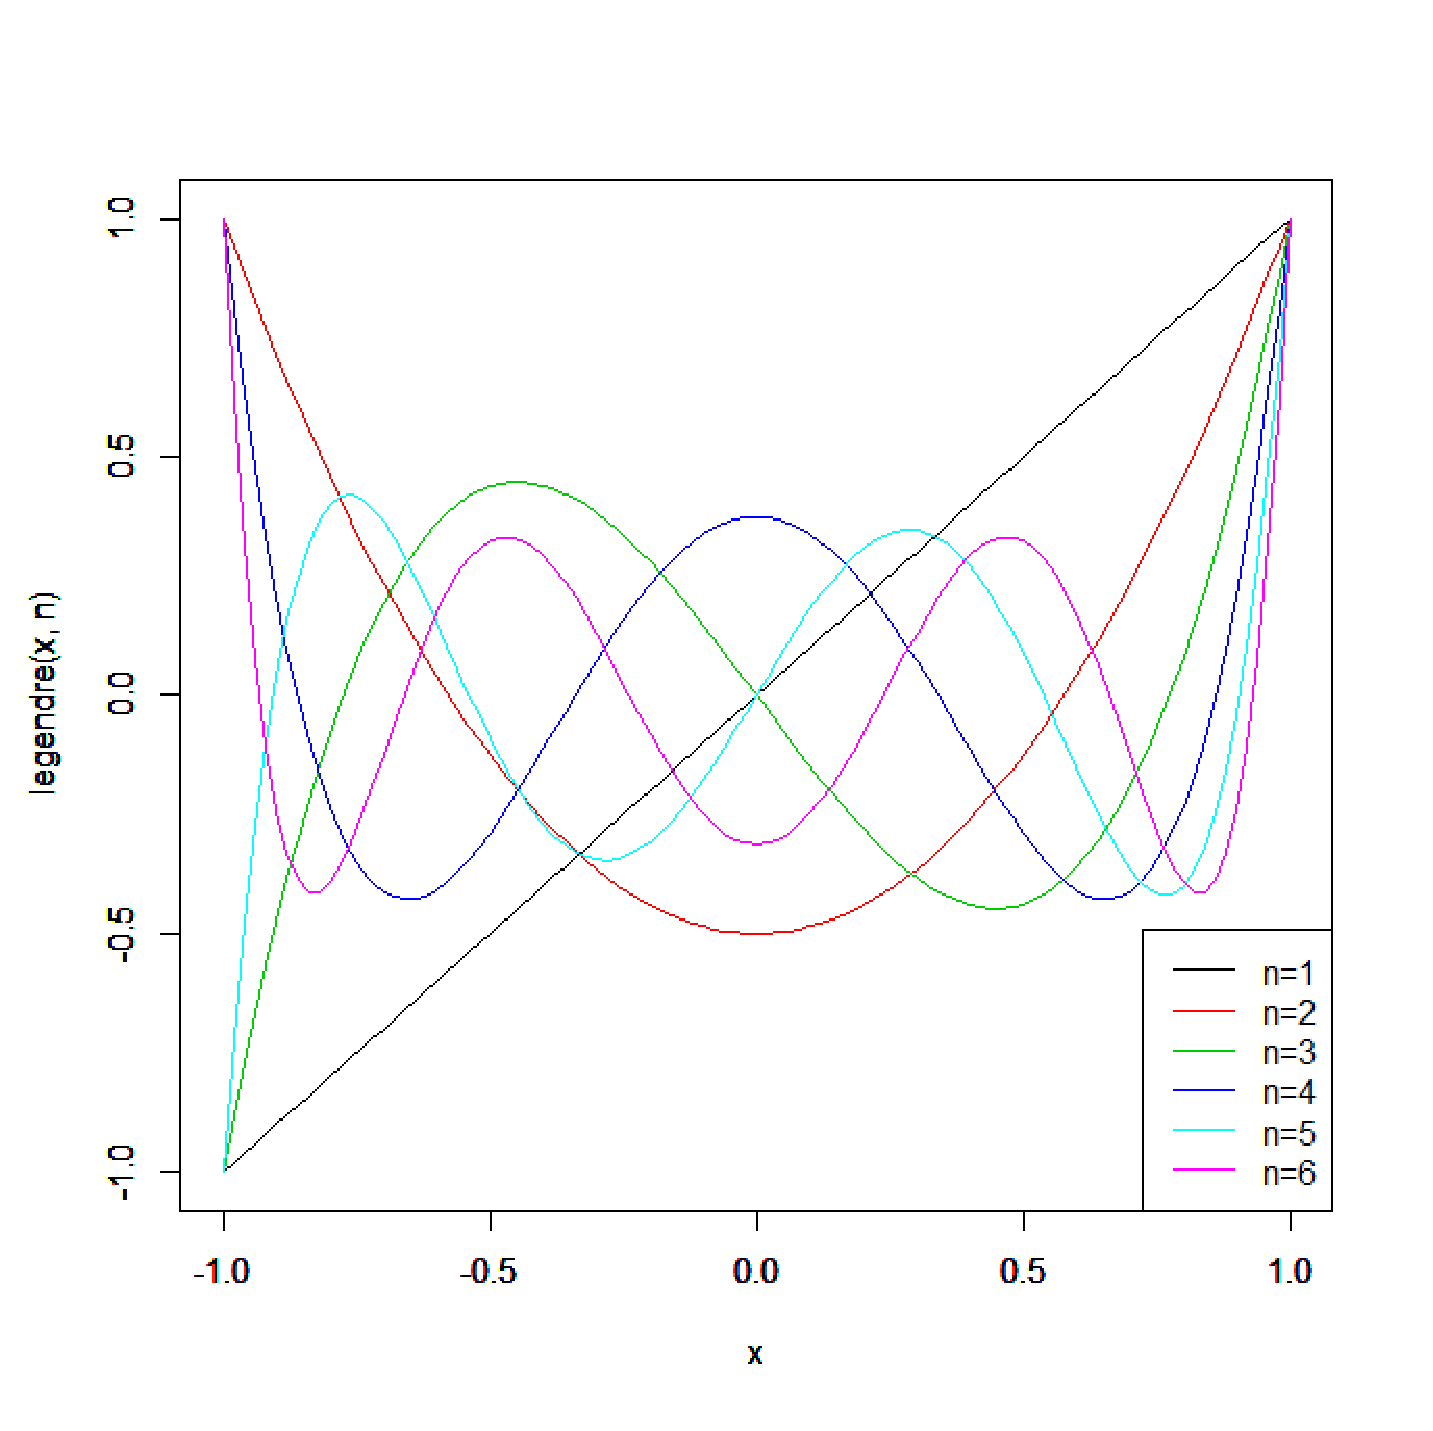
\includegraphics[clip,width = 10.0cm]{graphics/legendre.eps}
        \end{center}
        \caption{$n$次{\rm Legendre}多項式($n=1,2,3,4,5,6$)}
    \end{figure}
    \begin{lstlisting}[style=customR]
    factorial <- function(l) {
    	if (l==0) {
			return(1)
    	} else if (l > 0) {
			return(prod(1:l))
		}
	}
	
	legendre <- function(x, n) {
		sum <- 0
		for (k in 0:floor(n/2)) {
			numer <- factorial(2*n - 2*k) * (-1)^k * x^(n - 2*k)
			denom <- factorial(n - 2*k) * factorial(k) * factorial(n - k)
			sum <- sum + numer/denom
		}
		return(sum / 2^n)
	}
	
	for (n in 1:6) {
		curve(legendre(x, n), xlim = c(-1, 1), ylim = c(-1, 1), col=n)
		par(new=T)
	}
	
	legend("bottomright",
    	col=1:6, legend=c("n=1", "n=2", "n=3", "n=4", "n=5", "n=6"),
        lty = c(1,1,1,1,1,1))
    \end{lstlisting}
    
    式(\refeq{eq:legendre_generating})が$x$についても$w$についても解析的である下で,収束半径内では級数が広義一様収束するので,右辺の項別微分が正当化される.
    \begin{align}
    	\frac{d}{dw} \frac{1}{\sqrt{1 - 2wx + w^2}} &= \frac{x - w}{(1 - 2wx + w^2)^{3/2}} \\
        &= \sum_{n=1}^{\infty} n P_n(x) w^{n-1} \\
        &= \sum_{n=0}^{\infty} (n+1) P_{n+1}(x) w^n. \label{eq:legendre_w_derivative}
    \end{align}
    左辺の分母を元に戻すと,
    \begin{align}
    	\frac{x - w}{\sqrt{1 - 2wx + w^2}} = \sum_{n=0}^{\infty} (n+1) P_{n+1}(x) (1 - 2wx + w^2) w^n.
    \end{align}
    左辺と右辺と別々に計算しておくと,
    \begin{align}
    	\frac{x - w}{\sqrt{1 - 2wx + w^2}} &= x \sum_{n=0}^{\infty} P_n(x) w^n - \sum_{n=0}^{\infty} P_n(x)w^{n+1} \\
        &= x \sum_{n=0}^{\infty} P_n(x) w^n - \sum_{n=1}^{\infty} P_{n-1}(x) w^n \\
        &= x + x \sum_{n=1}^{\infty} P_n(x) w^n - \sum_{n=1}^{\infty} P_{n-1}(x) w^n.
    \end{align}
    \begin{align}
    	\sum_{n=0}^{\infty} (n+1) P_{n+1}(x) (1 - 2wx + w^2) w^n &= 
        \sum_{n=0}^{\infty} (n+1) P_{n+1}(x) w^n - 2x \sum_{n=0}^{\infty} (n+1) P_{n+1}(x) w^{n+1} + \sum_{n=0}^{\infty} (n+1) P_{n+1}(x) w^{n+2} \\
        &= \sum_{n=0}^{\infty} (n+1) P_{n+1}(x) w^n - 2x \sum_{n=1}^{\infty} n P_n(x) w^n + \sum_{n=2}^{\infty} (n-1) P_{n-1}(x) w^n \\
        &= x + \sum_{n=1}^{\infty} (n+1) P_{n+1}(x) w^n - 2x \sum_{n=1}^{\infty} n P_n(x) w^n + \sum_{n=1}^{\infty} (n-1) P_{n-1}(x) w^n.
    \end{align}
    右辺と左辺の$w^n$の項を比較することで,{\rm Legendre}多項式の漸化式を得る.
    \begin{screen}
    	\begin{description}
        	\item[{\rm Legendre}多項式の漸化式$1$]
            \begin{align}
            	(n+1)P_{n+1}(x) - (2n+1)xP_n(x) + nP_{n-1}(x) = 0, \quad (n \geq 1). \label{eq:legendre_recurrence1}
            \end{align}
        \end{description}
    \end{screen}
    
    先程は式(\refeq{eq:legendre_generating})を$w$について微分したが,次は$x$について微分する.$P_0$の微分が$0$になることに注意して,
    \begin{align}
    	\frac{d}{dx} \frac{1}{\sqrt{1 - 2wx + w^2}} = \frac{w}{(1 - 2wx + w^2)^{3/2}} = \sum_{n=0}^{\infty} P_n'(x) w^n (= \sum_{n=1}^{\infty} P_n'(x) w^n).
    \end{align}
    両辺に$x/w$を掛ける.
    \begin{align}
    	\frac{x}{\sqrt{(1 - 2wx + w^2)^{3/2}}} = \sum_{n=1}^{\infty} x P_n'(x) w^{n-1} = \sum_{n=0}^{\infty} x P_{n+1}'(x) w^n.
    \end{align}
    上二式の差と式(\refeq{eq:legendre_w_derivative})の$w^n$の項を照合すると次の関係を得る.
    \begin{align}
    	(n+1) P_{n+1}(x) = x P_{n+1}'(x) - P_n'(x), \quad (n = 0,1,2,3,\cdots). \label{eq:legendre_recurrence2}
    \end{align}
    式(\refeq{eq:legendre_recurrence1})を両辺$x$に関して微分する.
    \begin{align}
    	(n+1)P_{n+1}'(x) &- (2n+1)P_n(x) - (2n+1)xP_n'(x) + nP_{n-1}'(x) \\
        &= (n+1)P_{n+1}'(x) - (2n+1)P_n(x) - n(xP_n'(x) - P_{n-1}'(x))  - (n+1)xP_n'(x) \\
        &= (n+1) (P_{n+1}'(x) - xP_n'(x)) - (2n+1)P_n(x) - n^2 P_n(x) & (\because (\refeq{eq:legendre_recurrence2}))\\
        &= (n+1) \left(P_{n+1}'(x) - xP_n'(x) - (n+1)P_n(x)\right) = 0, \quad (n=0,1,2,3,\cdots).
    \end{align}
    最終段を式(\refeq{eq:legendre_recurrence1})によって変形する.
    \begin{align}
    	P_{n+1}'(x) - xP_n'(x) - (n+1)P_n(x) &= P_{n+1}'(x) - x\left(xP_{n+1}'(x) - (n+1) P_{n+1}(x)\right) - (n+1)P_n(x) \\
        &= (1-x^2) P_{n+1}'(x) + (n+1) \left(xP_{n+1}(x) - P_n(x)\right) = 0, \quad (n=0,1,2,3,\cdots).
    \end{align}
    この関係式は次節で扱うので目立たせておく.
    \begin{screen}
    	\begin{description}
        	\item[{\rm Legendre}多項式の漸化式$2$]
            \begin{align}
            	(1-x^2) P_{n+1}'(x) + (n+1) (xP_{n+1}(x) - P_n(x)) = 0, \quad (n \geq 0). \label{eq:legendre_recurrence2}
            \end{align}
        \end{description}
    \end{screen}
    
    続いて{\rm Legendre}多項式の直交性を証明する.{\rm Rodrigues}の公式(\refeq{eq:rodrigues})は微分で表現されているから,積分計算するのに便利である.
    $(x^2-1)^n$の$k (< n)$回微分の導関数の各項には$(x^2-1)$が残ることに注意して式変形を繰り返す.
    \begin{align}
    	\int_{-1}^{1} x^m P_n(x) dx &= \int_{-1}^{1} x^m \frac{1}{2^n n!} \frac{d^n}{dx^n}(x^2-1)^n\ dx \\
        &= \frac{1}{2^n n!} \left[ x^m \frac{d^{n-1}}{dx^{n-1}}(x^2-1)^n \right]_{-1}^{1} - \int_{-1}^{1} m x^{m-1} \frac{1}{2^n n!} \frac{d^{n-1}}{dx^{n-1}}(x^2-1)^n\ dx \\
        &= (-1) \left\{ \frac{1}{2^n n!} \left[m x^{m-1} \frac{d^{n-2}}{dx^{n-2}}(x^2-1)^n \right]_{-1}^{1} - \int_{-1}^{1} m(m-1) x^{m-2} \frac{1}{2^n n!} \frac{d^{n-2}}{dx^{n-2}}(x^2-1)^n\ dx \right\} \\
        &= (-1)^2 m(m-1) \int_{-1}^{1} x^{m-2} \frac{1}{2^n n!} \frac{d^{n-2}}{dx^{n-2}}(x^2-1)^n\ dx \\
        &= \cdots \\
        &= (-1)^k m(m-1)(m-2)\cdots(m-k+1) \int_{-1}^{1} x^{m-k} \frac{1}{2^n n!} \frac{d^{n-k}}{dx^{n-k}}(x^2-1)^n\ dx.
    \end{align}
    $m < n$であるなら,$k=m$として
    \begin{align}
    	(-1)^m m! \int_{-1}^{1} \frac{1}{2^n n!} \frac{d^{n-m}}{dx^{n-m}}(x^2-1)^n\ dx = (-1)^m m! \frac{1}{2^n n!} \left[ \frac{d^{n-m-1}}{dx^{n-m-1}}(x^2-1)^n \right]_{-1}^{1} = 0.
    \end{align}
    $m = n$であるなら,$k=n$として
    \begin{align}
    	(-1)^n n! \int_{-1}^{1} \frac{1}{2^n n!} \frac{d^0}{dx^0}(x^2-1)^n\ dx &= (-1)^n n! \frac{1}{2^n n!} \int_{-1}^{1} (x^2-1)^n\ dx \\
        &= (-1)^n n! \frac{1}{2^n n!} \left\{ \left[ x(x^2-1)^n \right]_{-1}^{1} - \int_{-1}^{1} 2nx^2 (x^2-1)^{n-1}\ dx \right\} \\
        &= (-1)^n n! \frac{1}{2^n n!} (-1) \left\{ \left[ 2n \frac{x^3}{3} (x^2-1)^{n-1} \right]_{-1}^{1} - \int_{-1}^{1} 2^2n(n-1)\frac{x^4}{3} (x^2-1)^{n-2}\ dx \right\} \\
        &= (-1)^n n! \frac{1}{2^n n!} (-1)^2 \int_{-1}^{1} 2^2n(n-1)\frac{x^4}{3} (x^2-1)^{n-2}\ dx \\
        &= \cdots \\
        &= (-1)^n n! \frac{1}{2^n n!} (-1)^k \int_{-1}^{1} 2^k n(n-1)(n-2)\cdots(n-k+1) \frac{x^{2k} 2^k k!}{(2k)!} (x^2-1)^{n-k}\ dx \\
        &= \cdots \\
        &= (-1)^n n! \frac{1}{2^n n!} (-1)^n 2^n n! \frac{2^n n!}{(2n)!} \int_{-1}^{1} x^{2n} dx \\
        &= n!^2 2^n \frac{1}{2^n n!} \frac{2^n n!}{(2n)!} \frac{2}{2n+1} \\
        &= \frac{n!^2 2^n}{(2n)!} \frac{2}{2n+1}.
    \end{align}
    以上の結果を用いれば次の計算が成り立つ.多項式の積であるから,最高次数が大きい方の{\rm Legendre}多項式はそのままに
    他方を項別に分解すれば先程の積分の結果を適用するだけである.最高次数が等しい場合,$n$次{\rm Legendre}多項式$P_n(x)$の$n$次の係数が
    $(2n)!/n!^2 2^n$であることに注意して,
    \begin{align}
    	\int_{-1}^{1} P_n(x)P_m(x)\ dx =
        \begin{cases}
        	0 \\
            \frac{(2n)!}{n!^2 2^n} \frac{n!^2 2^n}{(2n)!} \frac{2}{2n+1}
        \end{cases} =
        \begin{cases}
        	0, & m \neq n, \\
            \frac{2}{2n+1}, & m = n.
        \end{cases}
    \end{align}
    {\rm Kronecker delta}を用いれば次のように簡略表記もできる.
    \begin{screen}
    	\begin{description}
        \item[{\rm Legendre}多項式の直交性({\rm orthogonality})]\mbox{}\\
        	$n$次{\rm Legendre}多項式と$m$次{\rm Legendre}多項式の積の積分値は次のように表現される.$\delta_{nm}$は{\rm Kronecker delta}である.
    		\begin{align}
    			\int_{-1}^{1} P_n(x)P_m(x)\ dx = \frac{2}{2n+1} \delta_{nm}. \label{eq:legendre_orthogonality}
    		\end{align}
        \end{description}
    \end{screen}
    
    資料\cite{terakan}は{\rm Legendre}関数や{\rm Bessel}関数などの特殊関数の諸性質についてかなり多く書いてあるから,
    筆者も勉強してみたい.最後に$n$次{\rm Legendre}多項式の根の計算をしておく.各$n$に対して{\rm Legendre}多項式は一意に定まるので,
    根を一度計算しておけば{\rm Gauss-Legendre}則で用いるのに便利である.根の計算には{\rm Newton}法を用いる.初期値の設定が難しいが,
    東大の講義資料に載っていたものを使う.
    $n$次{\rm Legendre}多項式の$n$個の根を$\{y_i\}_{i=1}^{n}$と表現するとき,各$y_i$の特定に{\rm Newton}法を適用する際の初期値は
    \begin{align}
    	\cos{ \left( \frac{i-0.25}{n+0.5} \pi \right) }{}, \quad (i = 1,2,3,\cdots,n)
    \end{align}
    とおくと良い.また導関数の計算は式(\refeq{eq:legendre_recurrence2})を使う.多項式の根と積分の重み(次節参照)を計算し{\rm csv}ファイルに
    保存する{\rm C++}のソースコードを載せておく.
    再帰計算の打ち切り条件については,前の値との比較差が所定の値より小さくなった時点でループを抜ける.筆者が計算してみたところ,
    $n$が$40$を超える辺りで根が求められなくなった.ネット上には既に計算されたものも存在する.([ガウスルジャンドル積分]で検索すればおそらくヒットする.)
    より高精度な計算方法は筆者の力不足で実装できていない.
    \begin{lstlisting}[style=customCpp]
	#include <iostream>
	#include <cmath>
	#include <vector>
	#include <fstream>
	
	using namespace std;
	
	double factorial(int l) {
		if (l==0) {
			return 1.0;
		} else if (l >= 1) {
			double prod = 1.0;
			for (int i=1; i <= l; i++) {
				prod *= 1.0 * i;
			}
			return prod;
		}
	}
	
	double legendre(double x, int n) {
		double sum = 0.0;
		double numer = 0.0;
		double denom = 0.0;
		for (int k=0; k <= n/2; k++) {
			numer = factorial(2*(n-k)) * pow(-1, k) * pow(x, n-2*k);
			denom = factorial(n-2*k) * factorial(k) * factorial(n-k);
			sum += numer/denom;
		}
		return sum / pow(2, n);
	}
	
	double legendre_deriv(double x, int n) {
		return n * (x * legendre(x, n) - legendre(x, n-1)) / (x*x - 1);
	}
	
	vector<double> newton_method(int n) {
		vector<double> root;
		double x, tmp;
		for (int i=0; i<n; i++) {
			x = cos((i+0.75) * M_PI / (n+0.5));
			tmp = 1;
			while (abs(x-tmp) >= 1e-10) {
				tmp = x;
				x = x - legendre(x, n) / legendre_deriv(x, n);
			}
			root.push_back(x);
		}
		return root;
	}
	
	double gauss_legendre_weight(double y, int n) {
    	double denom = n*legendre(y, n-1);
    	return 2*(1-y*y) / (denom*denom);
	}
	
	int main() {
    	ofstream ofs("legendre_roots.csv");
    	vector<double> roots;
    	for (int n=1; n<=32; n++) {
        	roots = newton_method(n);
    		for (int i=0; i<n; ++i) {
    			ofs << n << "," << roots[i] << "," << gauss_legendre_weight(roots[i], n) << endl;
    		}
    	}
		return 0;
	}
    \end{lstlisting}
    
    {\rm Python}の{\rm numpy}は特殊関数も扱っていて,今回扱う多項式の根と積分の重みを計算してくれる.
    $80$次までの{\rm Legendre}多項式の根と重みを求めて{\rm csv}ファイルに保存する{\rm Python}スクリプトを紹介しておく.
    \begin{lstlisting}[style=customPython]
    from numpy.polynomial.legendre import leggauss
	import csv
	
	with open("legrootsweights.csv", mode='w') as f:
    	writer = csv.writer(f)
    	writer.writerow(['n', 'root', 'weight'])
    	for i in range(1, 81):
        	roots = leggauss(i)[0]
        	weights = leggauss(i)[1]
        	for j in range(0, i):
            	writer.writerow([i, "{0:.40f}".format(roots[j]), weights[j]])
    
    \end{lstlisting}

\subsection{{\rm Gauss-Legendre}則}
	\begin{itembox}[l]{教科書及びサイト}
    	{\rm ホームレスこ~よ~\cite{gauss_legendre}, 東大資料\cite{u_tokyo_legendre}}
    \end{itembox}
	$\mathbb{R}$の区間$I$上で可積分な実数値関数$f(x)$を区間$[a,b] \subset I$で積分する際,多項式近似で積分値の概算値を精度保証付きで計算する手法は
    この章のはじめに述べた.しかし台形則や{\rm Simpson}則による積分で精度良く計算すると分割数が多くなり,ただでさえ関数値の計算に時間が掛かる関数を
    広い区間で積分する際には,研究室の計算機をもってしても計算がなかなか終わらない.{\rm Gauss-Legendre}則において用いる{\rm Legendre}多項式は,
    その圧巻の験を発揮して計算の手間を減らし精度を上げる.その魅力溢れる計算の原理を以下に示す.
    \begin{align}
    	\int_{a}^{b} f(x) dx = \frac{b-a}{2} \int_{-1}^{1} f\left( \frac{b-a}{2}x + \frac{b+a}{2} \right) dx.
    \end{align}
    と変形して積分区間を$[-1, 1]$にする.便宜上以降の議論は
    \begin{align}
    	\int_{-1}^{1} f(x) dx
    \end{align}
    の積分を扱うこととする.
    $f(x)$の多項式近似に{\rm Legendre}多項式を使うので,この多項式が有つ根の性質を応用して次のことを考える.\\
    $n$次{\rm Legendre}多項式$P_n$の根を$y_1, y_2, \cdots, y_n$と表す.根はすべて異なる値で$(-1, 1)$の内点である.どの根とも異なる$1$点$y_0 \in (-1, 1)$を
    任意に指定すれば,$P_n$を{\rm Lagrange}補間の形式で表現できる.
    \begin{align}
    	P_n(y) &= \sum_{i=0}^{n} \prod_{\substack{j=0\\j \neq i}}^{n} \frac{y-y_j}{y_i - y_j} P_n(y_i) \\
        &= P_n(y_0) \prod_{\substack{j=1}}^{n} \frac{y-y_j}{y_0 - y_j} + \sum_{i=1}^{n} \prod_{\substack{j=0\\j \neq i}}^{n} \frac{y-y_j}{y_i - y_j} P_n(y_i) \\
        &= P_n(y_0) \prod_{\substack{j=1}}^{n} \frac{y-y_j}{y_0 - y_j}.
    \end{align}
    最右辺の相乗の項から$y_i$を任意に一つ選んで相乗の外に出す.
    \begin{align}
    	P_n(y) &= P_n(y_0) \prod_{\substack{j=1}}^{n} \frac{y-y_j}{y_0 - y_j} \\
        &= P_n(y_0) \frac{y - y_i}{y_0 - y_i} \prod_{\substack{j=1 \\ j \neq i}}^{n} \frac{y-y_j}{y_0 - y_j}.
    \end{align}
    同一な$n$次{\rm Legendre}多項式$P_n$の表現であるから,$y_0$の値に関係なく上の等式は成立する.従って$y_0$を$y_i$にいくらでも近づける極限操作$y_0 \to y_i$を考えて良い.
    ところで$P_n(y_i) = 0$であるから,右辺を$y_0 \to y_i$で極限を取ると微分の定義式になる.
    \begin{align}
    	P_n(y) &= \lim_{y_0 \to y_i} \frac{P_n(y_0) - P_n(y_i)}{y_0 - y_i} (y - y_i) \prod_{\substack{j=1 \\ j \neq i}}^{n} \lim_{y_0 \to y_i} \frac{y-y_j}{y_0 - y_j} \\
        &= P_n'(y_i) (y - y_i) \prod_{\substack{j=1 \\ j \neq i}}^{n} \frac{y-y_j}{y_i - y_j}. \label{eq:legendre_limit}
    \end{align}
    先程の$f(x)$を$2n - 1$次多項式$p_{2n-1}(x)$で{\rm Lagrange}補間する.$f$と$p_{2n-1}$が交わる$2n-1$個の点の中,
    $n$個は{\rm Legendre}多項式の根の位置で交わるようにする.$p_{2n - 1}$を{\rm Legendre}多項式$P_n$で割った商と余りは
    高々$n-1$次の多項式になるから,これを$q_{n-1}(x)$と$r_{n-1}(x)$と置く.
    \begin{align}
    	f(x) \approx p_{2n-1}(x) = P_n(x) q_{n-1}(x) + r_{n-1}(x).
    \end{align}
    両辺を積分すると,{\rm Legendre}多項式の直交性(\refeq{eq:legendre_orthogonality})により右辺第一項の積分値は$0$になる.
    \begin{align}
    	\int_{-1}^{1} p_{2n-1}(x) dx &= \int_{-1}^{1} P_n(x) q_{n-1}(x) dx + \int_{-1}^{1} r_{n-1}(x) dx \\
        &= \int_{-1}^{1} r_{n-1}(x) dx.
    \end{align}
    ここで$r_{n-1}(x)$を自身で{\rm Lagrange}補間する.ちなみに$r_{n-1}(x)$が$n-1$次多項式である保証はしていなかったが,
    $n$次{\rm Legendre}多項式の$n$個の根$\{y_i\}_{i=1}^{n}$を用いて$r_{n-1}$が$n-1$次の多項式であると証明できる.
    $f$と$p_{2n-1}$は$n$次{\rm Legendre}多項式の$n$個の根$\{y_i\}_{i=1}^{n}$で交わると約束したから,
    \begin{align}
    	f(y_i) = p_{2n-1} (y_i) = r_{n-1} (y_i), \quad (i = 1,2,3,\cdots,n)
    \end{align}
    が成り立ち,$r_{n-1}$は少なくとも$n$個の異なる点を通過するはずである.従って$r_{n-1}(x)$は一意に$n-1$次多項式と定まる.
    さて$r_{n-1}(x)$の{\rm Lagrange}補間は$n$次{\rm Legendre}多項式の$n$個の根$\{y_i\}_{i=1}^{n}$を使えばよく,
    \begin{align}
    	r_{n-1} (x) &= \sum_{i=1}^{n} r_{n-1}(y_i) \prod_{\substack{j=1 \\ j \neq i}}^{n} \frac{x-y_j}{y_i - y_j} \\
        &= \sum_{i=1}^{n} f(y_i) \prod_{\substack{j=1 \\ j \neq i}}^{n} \frac{x-y_j}{y_i - y_j} \\
    \end{align}
    と表現できる.式(\refeq{eq:legendre_limit})により更に変形する.
    \begin{align}
    	\sum_{i=1}^{n} f(y_i) \prod_{\substack{j=1 \\ j \neq i}}^{n} \frac{x-y_j}{y_i - y_j}
        &= \sum_{i=1}^{n} f(y_i) \frac{P_n(x)}{P_n'(y_i) (x - y_i)}.
    \end{align}
    従って積分は次の表現に書き換えられる.
    \begin{align}
    	\int_{-1}^{1} r_{n-1}(x) dx = \sum_{i=1}^{n} \frac{f(y_i)}{P_n'(y_i)} \int_{-1}^{1} \frac{P_n(x)}{x-y_i} dx.
    \end{align}
    ここで式(\refeq{eq:legendre_recurrence2})により
    \begin{align}
    	P_n'(y_i) = \frac{n\left( xP_n(y_i) - P_{n-1}(y_i) \right)}{y_i^2 - 1} = \frac{nP_{n-1}(y_i)}{1-y_i^2}.
    \end{align}
    が成り立つ.これを代入すれば
    \begin{align}
    	\int_{-1}^{1} r_{n-1}(x) dx &= \sum_{i=1}^{n} \frac{f(y_i)}{P_n'(y_i)} \int_{-1}^{1} \frac{P_n(x)}{x-y_i} dx \\
        &= \sum_{i=1}^{n} \frac{f(y_i) (1-y_i^2)}{nP_{n-1}(y_i)} \int_{-1}^{1} \frac{P_n(x)}{x-y_i} dx.
    \end{align}
    を得る.積分項を計算するために少し技巧的な操作を入れる.
    
    \begin{align}
    	Q_n(y) \equiv \int_{-1}^{1} \frac{P_n(x)}{y-x}dx
    \end{align}
    と置くと,漸化式(\refeq{eq:legendre_recurrence1})と直交性により
    \begin{align}
    	(n+1)Q_{n+1}(y) &= \int_{-1}^{1} \frac{(n+1)P_{n+1}(x)}{y-x}dx \\
        &= \int_{-1}^{1} \frac{1}{y-x}\left( (2n+1)xP_n(x) - nP_{n-1}(x) \right) dx \\
        &= \int_{-1}^{1} \frac{1}{y-x}\left( (2n+1)yP_n(x) - (2n+1)yP_n(x) + (2n+1)xP_n(x) - nP_{n-1}(x) \right) dx \\
        &= \int_{-1}^{1} \frac{1}{y-x}\left( (2n+1)yP_n(x) - nP_{n-1}(x) \right) dx - \int_{-1}^{1} P_n(x)dx \\
        &= (2n+1)y Q_n(y) - nQ_{n-1}(y)
    \end{align}
    が成り立つ.従って$Q_n$も漸化式(\refeq{eq:legendre_recurrence1})を満たすと示された.
    \begin{align}
    	(n+1)P_{n+1}(y) - (2n+1)yP_n(y) + nP_{n-1}(y) &= 0,\\
        (n+1)Q_{n+1}(y) - (2n+1)yQ_n(y) + nQ_{n-1}(y) &= 0
    \end{align}
    の第二項を消すと次の漸化式を得る.
    \begin{align}
    	(n+1)\left( P_{n+1}(y)Q_n(y) - P_n(y)Q_{n+1}(y) \right) &= n\left( P_n(y)Q_{n-1}(y) - P_{n-1}(y)Q_n(y) \right) \\
        &= (n-1)\left( P_{n-1}(y)Q_{n-2}(y) - P_{n-2}(y)Q_{n-1}(y) \right) \\
        &= (n-2)\left( P_{n-2}(y)Q_{n-3}(y) - P_{n-3}(y)Q_{n-2}(y) \right) \\
        &\cdots \\
        &= P_1(y)Q_0(y) - P_0(y)Q_1(y).
    \end{align}
    $P_0(y)=1, P_1(y)=y$であるから
    \begin{align}
    	P_1(y)Q_0(y) - P_0(y)Q_1(y) = y \int_{-1}^{1} \frac{1}{y-x}dx - \int_{-1}^{1} \frac{x}{y-x}dx = \int_{-1}^{1} dx = 2
    \end{align}
    となり
    \begin{align}
    	P_n(y)Q_{n-1}(y) - P_{n-1}(y)Q_n(y) = \frac{2}{n}
    \end{align}
    となる.ところで
    \begin{align}
    	P_n(y)Q_{n-1}(y) - P_{n-1}(y)Q_n(y) = \int_{-1}^{1} \frac{1}{y-x}\left( P_n(y)P_{n-1}(x) - P_{n-1}(y)P_n(x) \right) dx
    \end{align}
    であるから,ここに$y = y_i$を代入する.
    \begin{align}
    	\int_{-1}^{1} \frac{1}{y_i - x} \left( P_n(y_i) P_{n-1}(x) - P_{n-1} (y_i) P_n(x) \right)\ dx
        &= \int_{-1}^{1} \frac{P_{n-1} (y_i) P_n(x)}{x - y_i} dx = \frac{2}{n}.
    \end{align}
    従って
    \begin{align}
    	\int_{-1}^{1} r_{n-1}(x) dx &= \sum_{i=1}^{n} \frac{f(y_i) (1-y_i^2)}{nP_{n-1}(y_i)} \int_{-1}^{1} \frac{P_n(x)}{x-y_i} dx \\
        &= \sum_{i=1}^{n} \frac{f(y_i) (1-y_i^2)}{nP_{n-1}(y_i)} \frac{2}{n P_{n-1} (y_i)}.
    \end{align}
    以上をまとめると,{\rm Gauss-Legendre}則による積分の近似値は次のように表せる.
    \begin{align}
    	\int_{-1}^{1} f(x) dx \approx \sum_{i=1}^{n} \frac{2(1-y_i^2)}{ \left\{nP_{n-1}(y_i) \right\}^2} f(y_i).
    \end{align}
    はじめに提起した$[a, b]$上の積分値も次の式で計算することができる.
    
    \begin{screen}
    \begin{description}
    	\item[{\rm Gauss-Legendre}則]\mbox{}\\
        $f(x)$を$\mathbb{R}$の区間$I$上で可積分な実数値関数であるとする.$f(x)$の区間$[a,b] \subset I$の上での積分の近似値は次のように計算される.
        式中の$P_n(x)$は$n$次{\rm Legendre}多項式,$\{y_i\}_{i=1}^{n}$はその$n$個の実根である.
    		\begin{align}
    			\int_{a}^{b} f(x) dx &= \frac{b-a}{2} \int_{-1}^{1} f\left( \frac{b-a}{2}x + \frac{b+a}{2} \right) dx \\
        		&\approx \frac{b-a}{2} \sum_{i=1}^{n} \frac{2(1-y_i^2)}{ \left\{nP_{n-1}(y_i) \right\}^2} f\left( \frac{b-a}{2}y_i + \frac{b+a}{2} \right).
    		\end{align}
    \end{description}
    \end{screen}
    この積分の誤差評価であるが,現段階では手に負えないので割愛する.{\rm Wikipedia}を参照されたい.
    {\rm C++}で実装したものを載せておく.先程{\rm Python}で作成した{\rm legroootsweights.csv}から根と重みを取り出し積分値を計算するコードである.
    {\rm csv}ファイルを読み込む関数も載せておく.
    \begin{lstlisting}[style=customCpp]
    #include <iostream>
	#include <fstream>
	#include <sstream>
	#include <vector>
	#include <string>
    
    int stoi(string str) {
		int ret;
		stringstream ss;
		ss << str;
		ss >> ret;
		return ret;
	}

	double stod(string str) {
		double ret=0.0;
		stringstream ss;
		ss.str(str);
		ss >> ret;
		return ret;
	}
    
    vector<string> split(string& input, char delimiter) {
	    istringstream stream(input);
	    string field;
	    vector<string> result;
	    while (getline(stream, field, delimiter)) {
	        result.push_back(field);
	    }
	    return result;
	}

	vector<string> readcsv(string filepath, bool header) {
		string readline;
		ifstream ifs(filepath.c_str());
		vector<string> strvec;
		int p = 0;
		while(getline(ifs, readline)){
			if (header && p==0) {
				p++;
				continue;
			}
			strvec.push_back(readline);
		}
		return strvec;
	}
    
    double gauss_legendre(double (*func)(double *x), double lower, double upper, int n, int len, ...) {
		/*
		 * trapezoidal rule
		 * 可変長引数 ... は,関数が複数パラメータをもつ場合の対処
		 * n     : legendre多項式の次数
		 * len   : 被積分関数のパラメータの個数.なければ 0 を渡す.
		 * args  : 関数に渡す引数の配列
		 * sum   : 積分近似値
		 */
		double args[len+1];
		va_list ARGS;
		va_start(ARGS, len);
		if (len >= 1) {
			for (int i=1; i<=len; i++) {
				args[i] = va_arg(ARGS, double);
			}
		}
		va_end(ARGS);
		vector<string> strdata = readcsv("legrootsweights.csv", true);
		double root, weight, sum = 0.0;
		for (vector<string>::iterator itr = strdata.begin(); itr!=strdata.end(); ++itr) {
			if(n == stoi(split(*itr, ',').at(0))) {
				root = stod(split(*itr, ',').at(1));
				weight = stod(split(*itr, ',').at(2));
				args[0] = (upper - lower)*0.5*root + (upper + lower)*0.5;
				sum += weight * func(args);
			}
			if (n < stoi(split(*itr, ',').at(0))) {
				break;
			}
		}
		return sum * (upper - lower) * 0.5;
	}
    
    \end{lstlisting}

\subsection{{\rm Laguerre}多項式}
	前前節で直交多項式の一つ{\rm Legendre}多項式を扱ったが,{\rm Laguerre}多項式も亦た直交性を有つ.
    \begin{itembox}[l]{教科書及びサイト}
    	{\rm 寺澤寛一\cite{terakan}pp.147-149, 東大資料\cite{u_tokyo_legendre}}
    \end{itembox}
    
    \begin{screen}
    	\begin{description}
    		\item[{\rm Laguerre}多項式({\rm Laguerre polynomials})]
            \begin{align}
            	L_n(x) \equiv \exp{x} \frac{d^n}{dx^n} (x^n \exp{-x})
            \end{align}
            で定義される$n$次多項式$L_n$を{\rm Laguerre}多項式という.
    	\end{description}
    \end{screen}
    
    定義式を順次計算すれば具体的な多項式の形が判る.
    \begin{align}
    	\frac{d}{dx} x^n \exp{-x} &= n x^{n-1} \exp{-x} - x^n \exp{-x}, \\
        \frac{d^2}{dx^2} x^n \exp{-x} &= n(n-1) x^{n-2} \exp{-x} - n x^{n-1} \exp{-x} - n x^{n-1} \exp{-x} + x^n \exp{-x} \\
        	&= n(n-1) x^{n-2} \exp{-x} - 2n x^{n-1} \exp{-x} + x^n \exp{-x}, \\
        \frac{d^3}{dx^3} x^n \exp{-x} &= n(n-1)(n-2) x^{n-3} \exp{-x} - n(n-1) x^{n-2} \exp{-x} - 2n(n-1) x^{n-2} \exp{-x} \\
        	&\quad+ 2n x^{n-1} \exp{-x} + n x^{n-1} \exp{-x} - x^n \exp{-x} \\
            &\quad= n(n-1)(n-2) x^{n-3} \exp{-x} -3 n(n-1) x^{n-2} \exp{-x} + 3 n x^{n-1} \exp{-x} - x^n \exp{-x},
    \end{align}
    ここまで計算すれば大方の概形は見えてくる.即ち$k \leq n$に対して
    \begin{align}
    	\frac{d^k}{dx^k} x^n \exp{-x} &= \sum_{i=0}^{k} (-1)^{k-i} \binom{k}{i} n(n-1)(n-2)\cdots(n-i+1) x^{n-i} \exp{-x} \\
        &= \sum_{i=0}^{k} (-1)^{k-i} \binom{k}{i} \frac{n!}{(n-i)!} x^{n-i} \exp{-x} \label{eq:laguerre_k_deriv}
    \end{align}
    が成り立つと予想できる.帰納法によれば,$k<n$の下で
    \begin{align}
    	\frac{d^{k+1}}{dx^{k+1}} x^n \exp{-x} &= \frac{d}{dx} \sum_{i=0}^{k} (-1)^{k-i} \binom{k}{i} \frac{n!}{(n-i)!} x^{n-i} \exp{-x} \\
        &= \sum_{i=0}^{k} (-1)^{k-i} \binom{k}{i} \frac{n!}{(n-i)!} (n-i) x^{n-i-1} \exp{-x} 
        	- \sum_{i=0}^{k} (-1)^{k-i} \binom{k}{i} \frac{n!}{(n-i)!} x^{n-i} \exp{-x} \\
        &= \sum_{i=1}^{k+1} (-1)^{k-i+1} \binom{k}{i-1} \frac{n!}{(n-i)!} x^{n-i} \exp{-x}
         	- \sum_{i=0}^{k} (-1)^{k-i} \binom{k}{i} \frac{n!}{(n-i)!} x^{n-i} \exp{-x} \\
        &= \frac{n!}{(n-k-1)!} x^{n-k-1} \exp{-x} + \sum_{i=1}^{k} (-1)^{k-i+1} \binom{k}{i-1} \frac{n!}{(n-i)!} x^{n-i} \exp{-x} \\
        	&\quad + \sum_{i=1}^{k} (-1)^{k-i+1} \binom{k}{i} \frac{n!}{(n-i)!} x^{n-i} \exp{-x} + (-1)^{k+1} x^n \exp{-x} \\
        &= \frac{n!}{(n-k-1)!} x^{n-k-1} \exp{-x} + \sum_{i=1}^{k} (-1)^{k-i+1} \left( \binom{k}{i-1} + \binom{k}{i} \right) \frac{n!}{(n-i)!} x^{n-i} \exp{-x} 
        	+ (-1)^{k+1} x^n \exp{-x} \\
        &= \frac{n!}{(n-k-1)!} x^{n-k-1} \exp{-x} + \sum_{i=1}^{k} (-1)^{k-i+1} \binom{k+1}{i} \frac{n!}{(n-i)!} x^{n-i} \exp{-x} 
        	+ (-1)^{k+1} x^n \exp{-x} \\
        &= \sum_{i=0}^{k+1} (-1)^{k+1-i} \binom{k+1}{i} \frac{n!}{(n-i)!} x^{n-i} \exp{-x}
    \end{align}
    が成立するので先程の予想は正しい.従って{\rm Laguerre}多項式は
    \begin{align}
    	L_n(x) &= \sum_{i=0}^{n} (-1)^{n-i} \binom{n}{i} \frac{n!}{(n-i)!} x^{n-i} = \sum_{i=0}^{n} (-1)^{i} \binom{n}{i} \frac{n!}{i!} x^i
    \end{align}
    と表される.
    \begin{screen}
            \begin{Prop}
                $n$次{\rm Laguerre}多項式は$(0, \infty)$にことごとく異なる$n$個の実根を有つ.
        \end{Prop}
    \end{screen}
    \begin{Proof}
            順次微分の階数を上げていく.$k$階導関数を
        \begin{align}
                f_k(x) \equiv \exp{x}\frac{d^k}{dx^k} x^n\exp{-x}
        \end{align}
        と置く.任意の$k \leq n$に対して$f_k(x)$は$x$についての$n$次多項式であり,代数学の基本定理により$n$個の根を有つ.
        \begin{align}
                f_k(x) = \exp{x}\frac{d^k}{dx^k}(x^n\exp{-x}) = \sum_{i=0}^{k}(-1)^{k-i} \binom{k}{i} \frac{n!}{(n-i)!} x^{n-i}
        \end{align}
        は全ての項に$x$の$n-k$次以上の項を有つから,原点は$f_k$の$n-k$重根であることに注意する.また他の根は原点ではありえない.
        $f_k(x)$を$x^{n-k}$で除すときの商が正の定数項$n!/(n-k)!$を有つ為である.\\
        $k=1$のとき
            \begin{align}
                f_1(x) = \exp{x}\frac{d}{dx}(x^n\exp{-x}) = x^{n-1}(n-x)
        \end{align}
        は原点と$x=n$が零点となり,原点が$n-1$重根であるから根はこの二つで全てである.{\rm Rolle}の定理により$(0, n)$の内部に
        $f_2(a_{21}) = 0$なる$a_{21}$が存在する.$f_2(x)$の残りの根$a_{22}$は実根でなくてはならない.根を複素数で表す時,
        多項式の係数が全て実数であるなら根の共役複素数も亦た同じ多項式の根となるため$\overline{a_{22}}$も$f_2(x)$の根となるが,
        原点と$a_{21}$が$n$個の根の中の$n-1$個であるから$a_{22} = \overline{a_{22}}$とならねばならず,これは$a_{22}$が実数であることを示す.
        \begin{align}
                \frac{d}{dx}\frac{f_2(x)}{x^{n-2}}=-2\frac{f_1(x)}{x^{n-1}}
        \end{align}
        かつ$f_2(n) < 0$であるから$f_2(x)$の零点と$f_2'(x)$の零点は原点を除き一致しない.従って$f_2(x)$は原点の外に重根を持つことはない.
        $f_2(x)$にも{\rm Rolle}の定理を適用し,$f_3(a_{31})=0, f_3(a_{32})=0$を満たす
        $a_{31}\in (0, a_{11}), a_{32} \in (a_{11}, a_{12})$が存在することが判る.そして先ほどと同じ理由で$f_3(x)$の残り一つの根$a_{33}$も亦た実数である.
        また
        \begin{align}
                \frac{d}{dx}\frac{f_3(x)}{x^{n-3}}=-3\frac{f_2(x)}{x^{n-2}}
        \end{align}
        であり,$a_{31}$も$a_{32}$も$f_2(x)$の零点ではないから$f_3(x)$は原点を除き重根を有たない.
        従って$a_{33}$は$0$でも$a_{31}$でも$a_{32}$でもない実数である.
        $k=1,2,\cdots,n$で一般に
        \begin{align}
                \frac{d}{dx}\frac{f_k(x)}{x^{n-k}}=-k\frac{f_{k-1}(x)}{x^{n-k+1}}
        \end{align}
        が成り立つから,同様の議論を繰り返して,$f_k(x)\ (k \leq n)$の根が全て実数であり原点の外に重根は無いと判る.
        $n$次{\rm Laguerre}多項式$L_n(x) = f_n(x)$は原点を通らないから$(0, \infty)$に$n$個の悉く異なる実根を有つ.\qed
    \end{Proof}
    
    {\rm Laguerre}多項式も{\rm Legendre}多項式と同様に母関数を計算しておく.
    \begin{align}
    	\sum_{n=0}^{\infty} \frac{L_n(x)}{n!} t^n &= \sum_{n=0}^{\infty} \frac{1}{n!} \sum_{i=0}^{n} (-1)^{i} \binom{n}{i} \frac{n!}{i!} x^i t^n \\
        &= \sum_{i=0}^{\infty} \sum_{n=i}^{\infty} (-1)^{i} \frac{t^n}{i!} \binom{n}{i} x^i.
    \end{align}
    ここで負の二項展開を応用する.
    \begin{align}
    	\frac{1}{(1-t)^j} &= \sum_{r=0}^{\infty} \binom{n+j-1}{j-1} t^n = \sum_{n=j-1}^{\infty} \binom{n}{j-1} t^{n-j+1} \\
    	&\Rightarrow \frac{t^i}{(1-t)^{i+1}} = \sum_{n=i}^{\infty} \binom{n}{i} t^n
    \end{align}
    が成り立つ.元の式に戻れば,
    \begin{align}
    	\sum_{i=0}^{\infty} \sum_{n=i}^{\infty} (-1)^{i} \frac{t^n}{i!} \binom{n}{i} x^i
        = \sum_{i=0}^{\infty} \left( \sum_{n=i}^{\infty} \binom{n}{i} t^n \right) \frac{(-x)^i}{i!}
        = \sum_{i=0}^{\infty} \frac{1}{i!} \frac{(-xt)^i}{(1-t)^{i+1}}
        = \frac{1}{1-t} \exp{-xt/(1-t)}
    \end{align}
    となり母関数が導出される.$t$についての関数と見做すとき,収束半径が$1$であることに注意する.({\rm d'Alembert}の判定法か,分母に$1-t$が在ることから判る.)
    \begin{screen}
    	\begin{description}
        	\item[{\rm Laguerre}母関数({\rm Laguerre generating function})]
            \begin{align}
            	\frac{1}{1-t} \exp{-xt/(1-t)} = \sum_{n=0}^{\infty} \frac{L_n(x)}{n!} t^n, \quad (|t|<1)
            \end{align}
            で表現される左辺を{\rm Laguerre}母関数,右辺の$L_n(x)$を$n$次{\rm Laguerre}多項式と云う.
        \end{description}
    \end{screen}
    
    母関数を$x$について偏微分する.
    \begin{align}
    	\frac{\partial}{\partial x} \frac{1}{1-t} \exp{-xt/(1-t)} &= \frac{-t}{(1-t)^2} \exp{-xt/(1-t)} \\
        	&= -\frac{t}{1-t} \sum_{n=0}^{\infty} \frac{L_n(x)}{n!} t^n \\
            &= -\sum_{r=0}^{\infty} t^{r+1} \sum_{n=0}^{\infty} \frac{L_n(x)}{n!} t^n \\
            &= -\sum_{n=1}^{\infty} \sum_{r=0}^{n-1} \frac{L_r(x)}{r!} t^n. \label{eq:laguerre_x_partial1}
    \end{align}
    他方で母関数は$x$についての指数関数の展開であるから,収束半径は$\infty$であり項別微分が可能である.従って
    \begin{align}
    	\frac{\partial}{\partial x} \frac{1}{1-t} \exp{-xt/(1-t)} &= \sum_{n=0}^{\infty} \frac{L_n'(x)}{n!} t^n 
        = \sum_{n=1}^{\infty} \frac{L_n'(x)}{n!} t^n. & (\because L_0'(x)=0)\label{eq:laguerre_x_partial2}
    \end{align}
    式(\refeq{eq:laguerre_x_partial1})(\refeq{eq:laguerre_x_partial2})の$t^n$の係数を比較すれば次の関係を得る.
    \begin{align}
    	\frac{L_n'(x)}{n!} = -\sum_{r=0}^{n-1} \frac{L_r(x)}{r!} = \frac{L_{n-1}'(x)}{(n-1)!} - \frac{L_{n-1}(x)}{(n-1)!}, \quad (n=1,2,3,\cdots).
    \end{align}
    両辺を$n!$倍して一つの漸化式を得る.
    \begin{screen}
    	\begin{description}
        \item[{\rm Laguerre}多項式の漸化式$1$]
    		\begin{align}
    			L_n'(x) - n L_{n-1}'(x) + n L_{n-1}(x) = 0, \quad (n=1,2,3,\cdots). \label{eq:laguerre_recurrence1}
    		\end{align}
    	\end{description}
    \end{screen}
    
    同様に$t$についても母関数を偏微分する.
    \begin{align}
    	\frac{\partial}{\partial t} \frac{1}{1-t} \exp{-xt/(1-t)} &= \frac{1}{(1-t)^2} \exp{-xt/(1-t)} + \frac{1}{1-t}\frac{-x}{(1-t)^2} \exp{-xt/(1-t)} \\
        &= \frac{1-t-x}{(1-t)^2} \frac{1}{1-t} \exp{-xt/(1-t)}. \label{eq:laguerre_t_partial1}
    \end{align}
    母関数右辺も$|t|<1$の下では項別微分可能である.
    \begin{align}
    	\frac{\partial}{\partial t} \sum_{n=0}^{\infty} \frac{L_n(x)}{n!} t^n = \sum_{n=1}^{\infty} \frac{L_n(x)}{(n-1)!} t^{n-1}. \label{eq:laguerre_t_partial2}
    \end{align}
    式(\refeq{eq:laguerre_t_partial1})(\refeq{eq:laguerre_t_partial2})は同値であるから,(\refeq{eq:laguerre_t_partial1})の分母$(1-t)^2$を
    (\refeq{eq:laguerre_t_partial2})に移行して両式の係数を比較する.
    \begin{align}
    	(\refeq{eq:laguerre_t_partial1}) * (1-t)^2 &= (1-t-x) \frac{1}{1-t} \exp{-xt/(1-t)} \\
        	&= (1-t-x) \sum_{n=0}^{\infty} \frac{L_n(x)}{n!} t^n \\
            &= \sum_{n=0}^{\infty} \frac{L_n(x)}{n!} t^n - \sum_{n=0}^{\infty} \frac{L_n(x)}{n!} t^{n+1} - x \sum_{n=0}^{\infty} \frac{L_n(x)}{n!} t^n \\
            &= \sum_{n=0}^{\infty} \frac{L_n(x)}{n!} t^n - \sum_{n=1}^{\infty} \frac{L_{n-1}(x)}{(n-1)!} t^n - x \sum_{n=0}^{\infty} \frac{L_n(x)}{n!} t^n \\
            &= L_0(x) + L_1(x) t - L_0(x) t - x L_0(x) - x L_1(x)t \\
            	&\quad+ \sum_{n=2}^{\infty} \frac{L_n(x)}{n!} t^n - \sum_{n=2}^{\infty} \frac{L_{n-1}(x)}{(n-1)!} t^n - x \sum_{n=2}^{\infty} \frac{L_n(x)}{n!} t^n, \\
        (\refeq{eq:laguerre_t_partial2}) * (1-t)^2 &= (1-t)^2 \sum_{n=1}^{\infty} \frac{L_n(x)}{(n-1)!} t^{n-1} \\
        	&= (1-2t+t^2) \sum_{n=1}^{\infty} \frac{L_n(x)}{(n-1)!} t^{n-1} \\
            &= \sum_{n=1}^{\infty} \frac{L_n(x)}{(n-1)!} t^{n-1} - 2 \sum_{n=1}^{\infty} \frac{L_n(x)}{(n-1)!} t^n + \sum_{n=1}^{\infty} \frac{L_n(x)}{(n-1)!} t^{n+1} \\
            &= \sum_{n=0}^{\infty} \frac{L_{n+1}(x)}{n!} t^n - 2 \sum_{n=1}^{\infty} \frac{L_n(x)}{(n-1)!} t^n + \sum_{n=2}^{\infty} \frac{L_{n-1}(x)}{(n-2)!} t^n \\
            &= L_1(x) + L_2(x)t - 2L_1(x)t \\
            	&\quad+ \sum_{n=2}^{\infty} \frac{L_{n+1}(x)}{n!} t^n - 2 \sum_{n=2}^{\infty} \frac{L_n(x)}{(n-1)!} t^n + \sum_{n=2}^{\infty} \frac{L_{n-1}(x)}{(n-2)!} t^n.
    \end{align}
    $L_0(x) + L_1(x) t - L_0(x) t - x L_0(x) - x L_1(x)t = L_1(x) + L_2(x)t - 2L_1(x)t$であるから,$t^n(n \geq 2)$の係数を比較すれば次の関係を得る.
    \begin{align}
    	\frac{L_n(x)}{n!} - \frac{L_{n-1}(x)}{(n-1)!} - x \frac{L_n(x)}{n!} = \frac{L_{n+1}(x)}{n!} - 2 \frac{L_n(x)}{(n-1)!} + \frac{L_{n-1}(x)}{(n-2)!}.
    \end{align}
    両辺を$n!$倍して差を取れば二つ目の漸化式を得る.
    \begin{screen}
    	\begin{description}
        \item[{\rm Laguerre}多項式の漸化式$2$]
    		\begin{align}
    			L_{n+1}(x) - (2n+1-x) L_n(x) + n^2 L_{n-1}(x) = 0, \quad (n=1,2,3,\cdots). \label{eq:laguerre_recurrence2}
    		\end{align}
    	\end{description}
    \end{screen}
    漸化式(\refeq{eq:laguerre_recurrence2})の両辺を$x$について微分して移項する.
    \begin{align}
    	L_{n+1}'(x) = (2n+1-x) L_n'(x) - L_n(x) - n^2 L_{n-1}'(x).
    \end{align}
    漸化式(\refeq{eq:laguerre_recurrence1})を用いて上式の左辺と右辺第三項を変形する.
    \begin{align}
    	L_{n+1}'(x) &= (n+1)L_n'(x) - (n+1)L_n(x) \\
        &= (2n+1-x) L_n'(x) - L_n(x) - n^2 L_{n-1}'(x) \\
        &= (2n+1-x) L_n'(x) - L_n(x) - n^2 \left( \frac{1}{n}L_n'(x) + L_{n-1}(x) \right).
    \end{align}
    整理して$L_n'(x)$の項を左辺に移項すればもう一つの漸化式を得る.
    \begin{screen}
    	\begin{description}
        \item[{\rm Laguerre}多項式の漸化式$3$]
    		\begin{align}
    			xL_n'(x) = nL_n(x) - n^2 L_{n-1}(x), \quad (n=1,2,3,\cdots). \label{eq:laguerre_recurrence3}
    		\end{align}
    	\end{description}
    \end{screen}
    
    $L_n(x)$の直交性を示す.$[0, \infty)$を積分区間として,多項式の積に$\exp{-x}$を掛けてこれを被積分関数とする.導関数$\frac{d^k}{dx^k}(x^n \exp{-x}),\ (k<n)$
    の全ての項に$x\exp{-x}$が含まれていることはこの節の始めの帰納法で示した.従って以下の式で繰り返される部分積分の非積分項は$0$となる.
    \begin{align}
    	\int_{0}^{\infty} \exp{-x} L_m(x)L_n(x)dx &= \int_{0}^{\infty} L_m(x)\frac{d^n}{dx^n}(x^n \exp{-x})dx \\
        &= - \int_{0}^{\infty} L_m'(x)\frac{d^{n-1}}{dx^{n-1}}(x^n \exp{-x})dx \\
        &= (-1)^2 \int_{0}^{\infty} L_m''(x)\frac{d^{n-2}}{dx^{n-2}}(x^n \exp{-x})dx \\
        &\cdots \\
        &= (-1)^k \int_{0}^{\infty} L_m^{(k)}(x)\frac{d^{n-k}}{dx^{n-k}}(x^n \exp{-x})dx.
    \end{align}
    $m < n$である場合,$k=m$として
    \begin{align}
    	(-1)^m \int_{0}^{\infty} L_m^{(m)}(x)\frac{d^{n-m}}{dx^{n-m}}(x^n \exp{-x})dx &= m! \int_{0}^{\infty} \frac{d^{n-m}}{dx^{n-m}}(x^n \exp{-x})dx \\
        &= m! \left[ \frac{d^{n-m-1}}{dx^{n-m-1}}(x^n \exp{-x}) \right]_{0}^{\infty} = 0.
    \end{align}
    $m = n$である場合,$k=n$として
    \begin{align}
    	(-1)^n \int_{0}^{\infty} L_n^{(n)}(x)\frac{d^{n-n}}{dx^{n-n}}(x^n \exp{-x})dx &= n! \int_{0}^{\infty} x^n \exp{-x}dx = n! \Gamma(n+1) = (n!)^2.
    \end{align}
    \begin{screen}
    	\begin{description}
        \item[{\rm Laguerre}多項式の直交性({\rm orthogonality})]\mbox{}\\
        	$n$次{\rm Laguerre}多項式と$m$次{\rm Laguerre}多項式の積の積分値は次のように表現される.$\delta_{nm}$は{\rm Kronecker delta}である.
    		\begin{align}
    			\int_{0}^{\infty} \exp{-x} L_m(x)L_n(x)dx = m! n! \delta_{mn}, \quad (\delta: {\rm Kronecker\ delta}).
    		\end{align}
        \end{description}
    \end{screen}
    
    $n=m$の場合の積分値が$1$になるように正規化する.
    \begin{align}
    	1 = \int_{0}^{\infty} \exp{-x} L_n(x)L_n(x) \frac{1}{(n!)^2} dx = \int_{0}^{\infty} \left\{ \frac{L_n(x)}{n!} \exp{-x/2} \right\}^2 dx.
    \end{align}
    関数族$ \exp{-x/2} L_n(x) / n!, \quad (n \in \mathbb{N})$は$(0, \infty)$に於いて正規直交系を為す.正規化された{\rm Laguerre}関数のグラフの概形を
    示しておく.
    \begin{figure}[H]
        \begin{center}
    	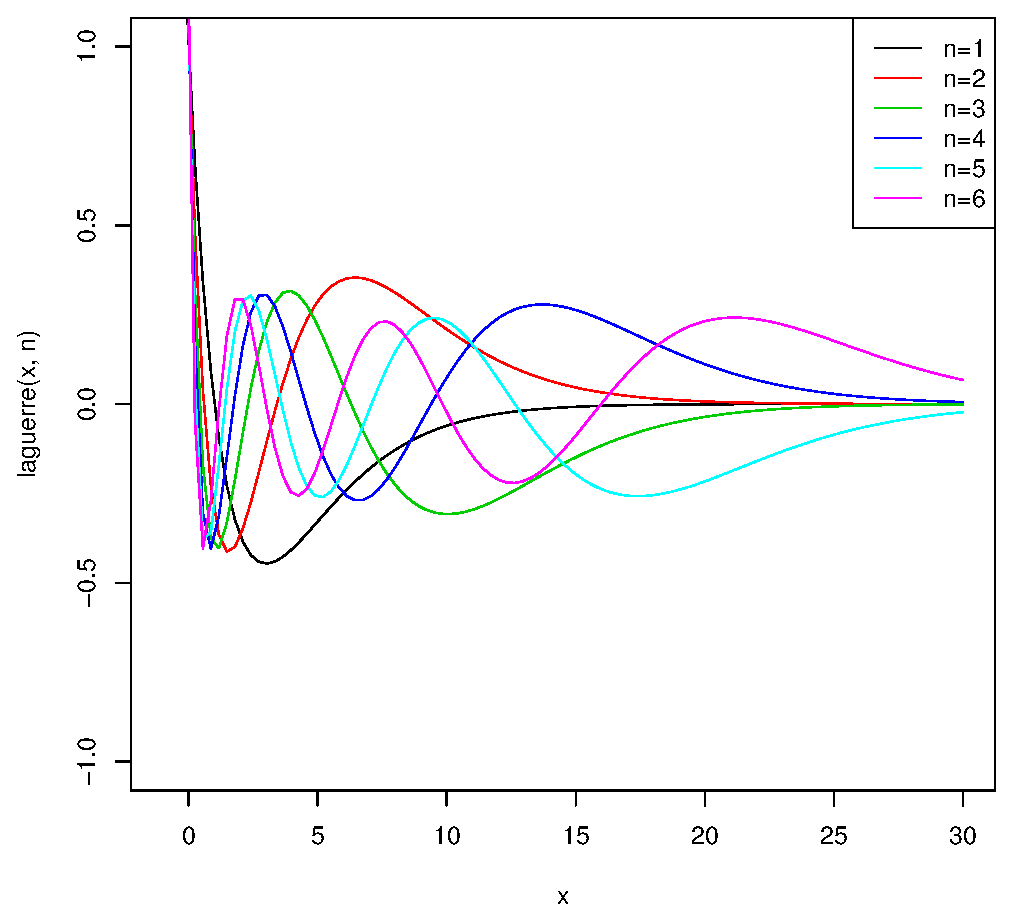
\includegraphics[clip,width = 10.0cm]{graphics/laguerre.eps}
        \end{center}
        \caption{$n$次{\rm Laguerre}多項式($n=1,2,3,4,5,6$)}
    \end{figure}
    \begin{lstlisting}[style=customR]
	combination <- function(n, r) {
	    if (r==0) {
	        return(1)
	    } else {
	        i <- 0:(r-1)
	        ret <- prod((n-i) / (i+1))
	        return(ret)
	    }
	}
	
	factorial <- function(l) {
	    if (l==0) {
	        return(1)
	    } else if (l > 0) {
	        return(prod(1:l))
	    }
	}
	
	laguerre <- function(x, n) {
	    s <- 0
	    for (r in 0:n) {
	        s <- s + (-1)^r * combination(n, r) * factorial(n) / factorial(r) * x^r
	    }
	    return(s * exp(-x/2) / factorial(n))
	}
	
	par(new=F)
	for (n in 1:4) {
	    curve(laguerre(x, n), xlim = c(-1, 30), ylim = c(-1, 1), col=n)
	    par(new=T)
	}
	
	legend("topright",
    	col=1:6, legend=c("n=1", "n=2", "n=3", "n=4", "n=5", "n=6"),
    	lty = c(1,1,1,1,1,1))
    \end{lstlisting}
    
    最後に$n$次{\rm Laguerre}多項式の根の計算をしておく.各$n$に対して{\rm Laguerre}多項式は一意に定まるので,
    根を一度計算しておけば{\rm Gauss-Laguerre}則で用いるのに便利である.根の計算には{\rm Newton}法を用いる.
    初期値の設定は{\rm Legendre}多項式の節と同じく東大の講義資料に載っていたものを使う.
    $n$次{\rm Laguerre}多項式の$n$個の根を$\{y_i\}_{i=1}^{n}$と表現するとき,各$y_i$の特定に{\rm Newton}法を適用する際の初期値は
    \begin{align}
    	\frac{\pi^2 \{i-0.25\}^2}{4n}, \quad (i = 1,2,3,\cdots,n)
    \end{align}
    とおく.また導関数の計算は式(\refeq{eq:laguerre_recurrence3})を使う.多項式の根と積分の重み(次節参照)を計算し{\rm csv}ファイルに保存する{\rm C++}のソースコードを載せておく.
    再帰計算の打ち切り条件については,前の値との比較差が所定の値より小さくなった時点でループを抜ける.筆者が計算してみたところ,
    $n$が$14$を超える辺りで根が求められなくなった.筆者の力不足で高精度な計算ができていない.積分計算に使う重みは信用ある計算センターの
    結果を拝借するべきである.
    \begin{lstlisting}[style=customCpp]
	#include <iostream>
	#include <cmath>
	#include <vector>
	#include <fstream>
	
	using namespace std;
	
	double factorial(int l) {
		if (l==0) {
			return 1.0;
		} else if (l >= 1) {
			double prod = 1.0;
			for (int i=1; i <= l; i++) {
				prod *= 1.0 * i;
			}
			return prod;
		}
	}
	
	double combination(int n, int i) {
		if (i==0) {
			return 1.0;
		} else {
			double prod = 1.0;
			for(int k=1; k<=i; ++k) {
				prod *= 1.0*(n-k+1)/k;
			}
			return prod;
		}
	}
	
	double laguerre(double x, int n) {
		double sum = 0.0;
		double comb;
		for (int i=0; i<=n; i++) {
			comb = combination(n, i);
			sum += pow(-x, i) * comb * comb * factorial(n-i);
		}
		return sum;
	}
	
	double laguerre_deriv(double x, int n) {
		return n * (laguerre(x, n) - n*laguerre(x, n-1)) / x;
	}
	
	vector<double> newton_method(int n) {
		vector<double> roots;
		double x, tmp;
		for (int i=0; i<n; i++) {
			x = M_PI*M_PI*(i+0.75)*(i+0.75) / (4*n);
			tmp = 1;
			while (abs(x-tmp) >= 1e-10) {
				tmp = x;
				x = x - laguerre(x, n) / laguerre_deriv(x, n);
			}
			roots.push_back(x);
		}
		return roots;
	}
	
	double gauss_laguerre_weight(double y, int n) {
    	double l = factorial(n) / laguerre(y, n+1);
    	return l*l*y;
	}
	
	int main() {
    	ofstream ofs("laguerre_roots.csv");
    	vector<double> roots;
    	for (int n=1; n<=15; n++) {
        	roots = newton_method(n);
    		for (int i=0; i<n; ++i) {
    			ofs << n << "," << roots[i] << "," << gauss_laguerre_weight(roots[i], n) << endl;
    		}
    	}
		return 0;
	}
    \end{lstlisting}
    
    $80$次までの{\rm Laguerre}多項式の根と重みを求めて{\rm csv}ファイルに保存する{\rm Python}スクリプトを紹介しておく.
    \begin{lstlisting}[style=customPython]
    from numpy.polynomial.laguerre import laggauss
	import csv
	
	with open("lagrootsweights.csv", mode='w') as f:
    	writer = csv.writer(f)
    	writer.writerow(['n', 'root', 'weight'])
    	for i in range(1, 81):
        	roots = laggauss(i)[0]
        	weights = laggauss(i)[1]
        	for j in range(0, i):
            	writer.writerow([i, "{0:.40f}".format(roots[j]), weights[j]])
    
    \end{lstlisting}

\subsection{{\rm Gauss-Laguerre}則}
	{\rm Gauss-Legendre}則と殆ど同様の議論で進むのでその節を参考すれば良い.{\rm Gauss-Legendre}則が有限区間での積分の近似に適用されたのに対し,
    この節では半無限区間での積分値を近似する.従ってここで扱うのは$[0, \infty)$で可積分な実数値関数$\exp{-x} f(x)$である.
    $n$次{\rm Laguerre}多項式の根$\{y_i\}_{i=1}^{n}$と後に導出する重み$w_i$を用いて
    \begin{align}
    	\int_{0}^{\infty} \exp{-x}f(x) dx = \sum_{i=1}^{n} w_i f(y_i)
    \end{align}
    なる形式で表現することを主意とする.\\
    $n$次{\rm Laguerre}多項式$L_n$のことごとく異なる$n$個の根$y_1, y_2, \cdots, y_n$は$(0, \infty)$の点である.{\rm Legendre}多項式の{\rm Lagrange}補間と
    全く同様に
    \begin{align}
    	L_n(y) = L_n'(y_i)(y - y_i)\prod_{\substack{j=1 \\ j \neq i}}^{n} \frac{y-y_j}{y_i-y_j}, \quad (y_i \in \{y_r\}_{r=1}^{n})
    \end{align}
    と表現できる.
    次に$f(x)$を$2n-1$次多項式$p_{2n-1}(x)$で{\rm Lagrange}補間する.$p_{2n-1}(x)$は$L_n(x)$の根$y_1, y_2, \cdots, y_n$に於いては$f(y_1), f(y_2), \cdots, f(y_n)$
    を通過するものとする.$p_{2n-1}(x)$を$L_n(x)$で割った商と余りの多項式を$q_{n-1}(x), r_{n-1}(x)$と置く.
    \begin{align}
    	f(x) \approx p_{2n-1}(x) = L_n(x)q_{n-1}(x) + r_{n-1}(x).
    \end{align}
    両辺を$[0, \infty)$で広義積分する.{\rm Laguerre}多項式の直交性により,右辺第一項の積分値は$0$になる.
    \begin{align}
    	\int_{0}^{\infty} \exp{-x}p_{2n-1}(x) dx &= \int_{0}^{\infty} \exp{-x}L_n(x)q_{n-1}(x) dx + \int_{0}^{\infty} \exp{-x}r_{n-1}(x) dx \\
        &= \int_{0}^{\infty} \exp{-x}r_{n-1}(x) dx.
    \end{align}
    $r_{n-1}(x)$は{\rm Gauss-Legendre}則の節での証明により$n-1$次多項式であると判っている.$L_n(x)$の全ての根において$f(y_i)=r_{n-1}(y_i)$
    が成り立つので,根$\{y_i\}_{i=1}^{n}$を用いて$r_{n-1}(x)$を{\rm Lagrange}補間する.
    \begin{align}
    	r_{n-1}(x) &= \sum_{i=1}^{n} f(y_i) \prod_{\substack{j=1 \\ j \neq i}}^{n} \frac{x-y_j}{y_i-y_j} \\
        &= \sum_{i=1}^{n} f(y_i) \frac{L_n(x)}{L_n'(y_i)(x-y_i)}.
    \end{align}
    計算するべき積分は
    \begin{align}
    	\int_{0}^{\infty} \exp{-x}r_{n-1}(x) dx &= \sum_{i=1}^{n} \frac{f(y_i)}{L_n'(y_i)} \int_{0}^{\infty} \exp{-x} \frac{L_n(x)}{x-y_i}dx \\
        &= \sum_{i=1}^{n} f(y_i) \frac{y_i}{L_{n+1}(y_i)} \int_{0}^{\infty} \exp{-x} \frac{L_n(x)}{x-y_i}dx 
        	& (\because (\refeq{eq:laguerre_recurrence1}),(\refeq{eq:laguerre_recurrence3}))
    \end{align}
    と表現される(式(\refeq{eq:laguerre_recurrence3})にて$n$を$n+1$にして$x=y_i$を代入し式(\refeq{eq:laguerre_recurrence1})で$n$を$n+1$とすればよい).
    {\rm Gauss-Legendre}則の節と同様に
    \begin{align}
    	Q_n(y) \equiv \int_{0}^{\infty} \exp{-x} \frac{L_n(x)}{y-x} dx
    \end{align}
    と置く.漸化式(\refeq{eq:laguerre_recurrence2})と直交性により
    \begin{align}
    	Q_{n+1}(y) &= \int_{0}^{\infty} \exp{-x} \frac{L_{n+1}(x)}{y-x} dx \\
        &= \int_{0}^{\infty} \exp{-x} \frac{1}{y-x} \left( (2n+1-x)L_n(x) - n^2L_{n-1}(x) \right) dx \\
        &= \int_{0}^{\infty} \exp{-x} \frac{1}{y-x} \left( (2n+1-y)L_n(x) - (2n+1-y)L_n(x) + (2n+1-x)L_n(x) - n^2L_{n-1}(x) \right) dx \\
        &= \int_{0}^{\infty} \exp{-x} \frac{1}{y-x} \left( (2n+1-y)L_n(x) - n^2L_{n-1}(x) \right) dx + \int_{0}^{\infty} \exp{-x} L_n(x) dx \\
        &= (2n+1-y)Q_n(y) - n^2Q_{n-1}(y)
    \end{align}
    が成り立つ.従って$Q_n$も漸化式(\refeq{eq:laguerre_recurrence2})を満たすと示された.
    \begin{align}
    	L_{n+1}(y) - (2n+1-y)L_n(y) + n^2L_{n-1}(y) &= 0, \\
        Q_{n+1}(y) - (2n+1-y)Q_n(y) + n^2Q_{n-1}(y) &= 0
    \end{align}
    の第二項を消すと次の漸化式を得る.
    \begin{align}
    	L_{n+1}(y) Q_n(y) - L_n(y) Q_{n+1}(y) &= n^2 \left( L_n(y) Q_{n-1}(y) - L_{n-1}(y) Q_n(y) \right) \\
        &= n^2 (n-1)^2 \left( L_{n-1}(y) Q_{n-2}(y) - L_{n-2}(y) Q_{n-1}(y) \right) \\
        &= n^2 (n-1)^2 (n-2)^2 \left( L_{n-2}(y) Q_{n-3}(y) - L_{n-3}(y) Q_{n-2}(y) \right) \\
        &\cdots \\
        &= (n!)^2 \left( L_1(y) Q_0(y) - L_0(y) Q_1(y) \right).
    \end{align}
    $L_0(y)=1, L_1(y)=-y+1$であるから
    \begin{align}
    	L_1(y) Q_0(y) - L_0(y) Q_1(y) &= (-y+1) \int_{0}^{\infty} \exp{-x} \frac{1}{y-x} dx - \int_{0}^{\infty} \exp{-x} \frac{-x+1}{y-x} dx \\
        &= - \int_{0}^{\infty} \exp{-x} dx \\
        &= -1
    \end{align}
    となり
    \begin{align}
    	L_{n+1}(y) Q_n(y) - L_n(y) Q_{n+1}(y) = -(n!)^2
    \end{align}
    となる.ところで
    \begin{align}
    	L_{n+1}(y) Q_n(y) - L_n(y) Q_{n+1}(y) = \int_{0}^{\infty} \exp{-x} \frac{1}{y-x} \left( L_{n+1}(y)L_n(x) - L_n(y)L_{n+1}(x) \right) dx
    \end{align}
    であるから,ここに$y=y_i$を代入する.
    \begin{align}
    	\int_{0}^{\infty} \exp{-x} \frac{1}{y_i-x} \left( L_{n+1}(y_i)L_n(x) - L_n(y_i)L_{n+1}(x) \right) dx 
        = \int_{0}^{\infty} \exp{-x} \frac{1}{y_i-x} L_{n+1}(y_i)L_n(x) dx = -(n!)^2.
    \end{align}
    従って
    \begin{align}
    	\int_{0}^{\infty} \exp{-x} r_{n-1}(x) dx
        &= \sum_{i=1}^{n} f(y_i) \frac{y_i}{L_{n+1}(y_i)} \int_{0}^{\infty} \exp{-x} \frac{L_n(x)}{x-y_i}dx \\
        &= \sum_{i=1}^{n} f(y_i) \frac{y_i}{L_{n+1}(y_i)} \frac{(n!)^2}{L_{n+1}(y_i)} \\
        &= \sum_{i=1}^{n} f(y_i) \frac{(n!)^2 y_i}{\left\{L_{n+1}(y_i)\right\}^2}.
    \end{align}
    
    \begin{screen}
    \begin{description}
    	\item[{\rm Gauss-Laguerre}則]\mbox{}\\
        $[0, \infty)$で定義される実数値関数$f(x)$について,$\exp{-x}f(x)$が$[0, \infty)$の上で可積分であるならその積分は次の式で近似される.
        式中の$L_n(x)$は$n$次{\rm Laguerre}多項式,$\{y_i\}_{i=1}^{n}$はその$n$個の実根である.
    		\begin{align}
    			\int_{0}^{\infty} \exp{-x} f(x) dx \approx \sum_{i=1}^{n} f(y_i) \frac{(n!)^2 y_i}{\left\{L_{n+1}(y_i)\right\}^2}.
    		\end{align}
    \end{description}
    \end{screen}
    
\subsection{{\rm Chebyshev}多項式}
	\begin{itembox}[l]{教科書及びサイト}
    	{\rm Carnahan, Luther, Wilkes\cite{numerical_calculation}pp.71-74.}
    \end{itembox}
    \begin{screen}
    	\begin{description}
        	\item[{\rm Chebyshev}多項式({\rm Chebyshev polynomials})]\mbox{}\\
            次の式で定義される関数を$n$次の{\rm Chebyshev}多項式という.$n = 0,1,2,\cdots$,$-1 \leq x \leq 1$の下で,
            \begin{align}
            	T_n(x) \equiv \cos{(n\cos{x}{-1})}{}.
            \end{align}
        \end{description}
    \end{screen}
    定義式が$x$の$n$次多項式であるとは判然しないが,精しく述べる.
    \begin{align}
    	T_0(x) &= \cos{0}{} = 1, \\
        T_1(x) &= \cos{\cos{x}{-1}}{} = x,
    \end{align}
    であることはすぐに判る.$\theta = \cos{x}{-1}$とおくと見通しが良くなる.{\rm Euler}の関係式により
    \begin{align}
    	\cos{n\theta}{} = \frac{\exp{in\theta} + \exp{-in\theta}}{2}
    \end{align}
    と書き表せる.ここで
    \begin{align}
    	(\exp{i(n-1)\theta} + \exp{-i(n-1)\theta})(\exp{i\theta} + \exp{-i\theta}) = \exp{in\theta} + \exp{-in\theta} + \exp{i(n-2)\theta} + \exp{-i(n-2)\theta}
    \end{align}
    と計算できるから,{\rm cos}で表現すると
    \begin{align}
    	\cos{(n-1)\theta}{}\cos{\theta}{} = \frac{1}{2}(\cos{n\theta}{} + \cos{(n-2)\theta}{})
    \end{align}
    が成り立つ.こうして一つの漸化式を得る.
    \begin{screen}
    	\begin{description}
        	\item[{\rm Chebyshev}多項式の漸化式]
            \begin{align}
            	T_{n+2}(x) = 2xT_{n+1}(x) - T_{n}(x), \quad (n=0,1,2,\cdots,\ -1 \leq x \leq 1). \label{eq:chebyshev_recurrence}
            \end{align}
        \end{description}
    \end{screen}
    漸化式を使えば,$T_2(x)$が$x$の$2$次多項式,$T_3(x)$が$x$の$3$次多項式,$\cdots$,$T_n(x)$が$x$の$n$次多項式,であることが帰納的に判明する.
    \begin{align}
    	T_0(x) &= 1, \\
        T_1(x) &= x, \\
        T_2(x) &= 2x^2 - 1, \\
        T_3(x) &= 4x^3 - 3x, \\
        T_4(x) &= 8x^4 - 8x^2 + 1, \\
        T_5(x) &= 16x^5 - 20x^3 + 5x, \\
        T_6(x) &= 32x^6 -48x^4 + 18x^2 -1, \\
        &\vdots
    \end{align}
    $\cos{\theta}{} = x$と置いたから,$0 \leq \theta \leq \pi$で考えれば$\cos{n\theta}{}$の零点がちょうど$n$個求まる.
    \begin{align}
    	\theta = \frac{2i-1}{2n}\pi, \quad (i=1,2,\cdots,n).
    \end{align}
    つまり$T_n(x)$の$n$個の根($\{y_i\}_{i=1}^{n}$と表す)は全て$-1 \leq x \leq 1$の中に存在し,
    \begin{align}
    	y_i = \cos{\left( \frac{2i-1}{2n}\pi \right)}{}, \quad (i=1,2,\cdots,n),
    \end{align}
    と表される.
    次図に$6$次までの{\rm Chebyshev}多項式の概形を示す.
    \begin{figure}[H]
        \begin{center}
    	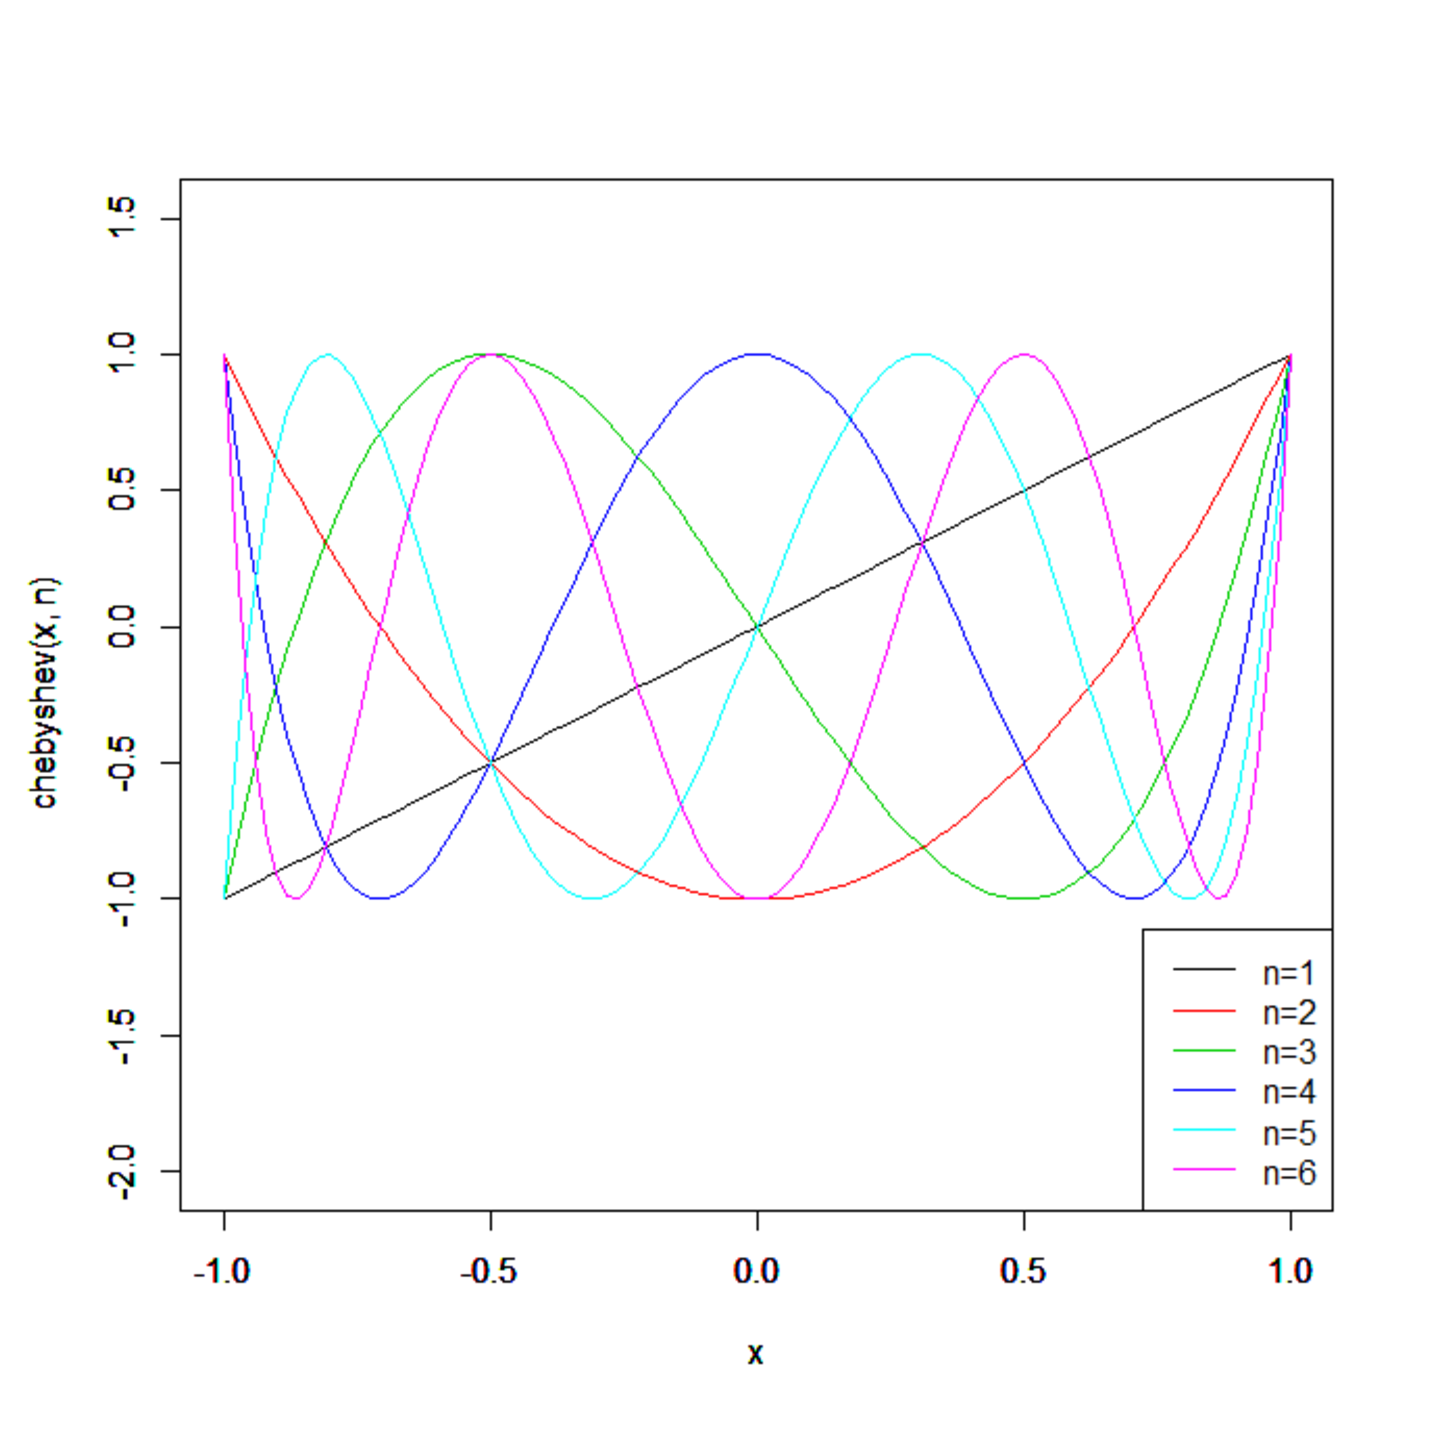
\includegraphics[clip,width = 10.0cm]{graphics/chebyshev.eps}
        \end{center}
        \caption{$n$次{\rm Chebyshev}多項式($n=1,2,3,4,5,6$)}
    \end{figure}
    \begin{lstlisting}[style=customR]
	chebyshev <- function(x, n) {
    	return(cos(n * acos(x)))
	}
	
	for (n in 1:6) {
    	curve(chebyshev(x, n), xlim = c(-1, 1), ylim = c(-2, 1.5), col=n)
    	par(new=T)
	}
	
	legend("bottomright",
    	col=1:6, legend=c("n=1", "n=2", "n=3", "n=4", "n=5", "n=6"),
    	lty = c(1,1,1,1,1,1))
	\end{lstlisting}
    
    {\rm Chebyshev}多項式もまた直交多項式の一つである.以降で直交性を利用した{\rm Gauss}型積分が定義される.
    \begin{align}
    	\int_{-1}^{1} \frac{1}{\sqrt{1-x^2}}T_n(x)T_m(x)dx &= \int_{-1}^{1} \frac{1}{\sqrt{1-x^2}} \cos{(n\cos{x}{-1})}{}\cos{(m\cos{x}{-1})}{} dx \\
        &= \int_{0}^{\pi} \frac{1}{\sin{\theta}{}} \cos{n\theta}{}\cos{m\theta}{} \sin{\theta}{} d\theta \\
        &= \int_{0}^{\pi} \cos{n\theta}{}\cos{m\theta}{} d\theta.
    \end{align}
    $n=m=0$の場合積分値は$\pi$となる.その他の場合について,式変形を続ける.
    \begin{align}
    	\int_{0}^{\pi} \cos{n\theta}{}\cos{m\theta}{} d\theta &= \int_{0}^{\pi} \frac{\cos{(n+m)\theta}{} + \cos{(n-m)\theta}{}}{2} d\theta \\
        &= \begin{cases}
        	\frac{1}{2} \left[ \frac{1}{n+m} \sin{(n+m)\theta}{} + \frac{1}{n-m} \sin{(n-m)\theta}{} \right]_{0}^{\pi} & (n \neq m) \\
            \frac{1}{2} \left[ \frac{1}{2n} \sin{2n\theta}{} + \theta \right]_{0}^{\pi} & (n=m)
        	\end{cases} \\
        &= \begin{cases}
        	0 & (n \neq m) \\
            \frac{\pi}{2} & (n=m)
            \end{cases}.
    \end{align}
    
    \begin{screen}
    	\begin{description}
        	\item[{\rm Chebyshev}多項式の直交性]\mbox{}\\
            任意の$n,m \in \{0,1,2,3,\cdots\}$次の{\rm Chebyshev}多項式$T_n(x), T_m(x)$に対して次の関係が成立する.
            \begin{align}
            	\int_{-1}^{1} \frac{1}{\sqrt{1-x^2}}T_n(x)T_m(x)dx = 
                \begin{cases}
                	\pi & (n=m=0) \\
                    \frac{\pi}{2} & (n = m \neq 0) \\
                    0 & (n \neq m)
                \end{cases}.
            \end{align}
        \end{description}
    \end{screen}
    任意の$n$次多項式は$n$次以下の{\rm Chebyshev}多項式の一次結合で表される({\rm Legendre}多項式の節の定理を参照)ので,$T_m(x),\ (m \geq 1)$と
    $m-1$次以下の任意の多項式との積の積分も上と同様の結果を得る.

\subsection{{\rm Gauss-Chebyshev}則}
	{\rm Gauss-Legendre}則,{\rm Gauss-Laguerre}則の場合と殆ど同様の議論で進む.考えるのは区間$[-1,1]$上の実数値関数$f(x)$の積分である.
    $n$次{\rm Chebyshev}多項式の根$\{y_i\}_{i=1}^{n}$と後述する重み$\{w_i\}_{i=1}^{n}$を用いて
    \begin{align}
    	\int_{-1}^{1} \frac{1}{\sqrt{1-x^2}} f(x) dx = \sum_{i=1}^{n} w_i f(y_i) \label{eq:gauss_chebyshev_model}
    \end{align}
    なる形式で表現することを主意とする.積分区間が有限区間であれば,下式のように適当な変数変換をして上の形式で表現できる.
    \begin{align}
    	\int_{a}^{b} f(x)dx &= \frac{b-a}{2} \int_{-1}^{1} f\left( \frac{b-a}{2}x + \frac{b+a}{2} \right) dx \\
        &= \frac{b-a}{2} \int_{-1}^{1} \frac{1}{\sqrt{1-x^2}} \sqrt{1-x^2} f\left( \frac{b-a}{2}x + \frac{b+a}{2} \right) dx \\
        &= \frac{b-a}{2} \sum_{i=1}^{n} w_i \sqrt{1-y_i^2} f\left( \frac{b-a}{2}y_i + \frac{b+a}{2} \right).
    \end{align}
    $n$次{\rm Chebshev}多項式$T_n$のことごとく異なる$n$個の根$\{y_i\}_{i=1}^{n}$は全て$(-1,1)$の内点である.{\rm Legendre}多項式の{\rm Lagrange}補間と全く同様に
    \begin{align}
    	T_n(y) = T_n'(y_i)(y - y_i)\prod_{\substack{j=1 \\ j \neq i}}^{n} \frac{y-y_j}{y_i - y_j}, \quad(y_i \in \{y_r\}_{r=1}^{n})
    \end{align}
    と表現できる.次に式(\refeq{eq:gauss_chebyshev_model})に於ける$f(x)$を$2n-1$次多項式$p_{2n-1}(x)$で{\rm Lagrange}補間する.$p_{2n-1}(x)$
    は$T_n(x)$の根$y_1, y_2, \cdots, y_n$に於いては$f(y_1), f(y_2), \cdots, f(y_n)$を通過するものとする.$p_{2n-1}(x)$を$T_n(x)$で割った商と余りの多項式を
    $q_{n-1}(x), r_{n-1}(x)$と置く.
    \begin{align}
    	f(x) \approx p_{2n-1}(x) = T_n(x)q_{n-1}(x) + r_{n-1}(x).
    \end{align}
    両辺を$[-1,1]$で積分する.{\rm Chebyshev}多項式の直交性により,右辺第一項の積分値は$0$になる.
    \begin{align}
    	\int_{-1}^{1} \frac{1}{\sqrt{1-x^2}} p_{2n-1}(x) dx 
        &= \int_{-1}^{1} \frac{1}{\sqrt{1-x^2}} T_n(x)q_{n-1}(x) dx + \int_{-1}^{1} \frac{1}{\sqrt{1-x^2}} r_{n-1}(x) dx \\
        &= \int_{-1}^{1} \frac{1}{\sqrt{1-x^2}} r_{n-1}(x) dx.
    \end{align}
    $r_{n-1}(x)$は{\rm Gauss-Legendre}則の節での証明により$n-1$次多項式であると判っている.$T_n(x)$の全ての根において
    $f(y_i) = r_{n-1}(y_i)$が成り立つので,根$\{y_i\}_{i=1}^{n}$を用いて$r_{n-1}(x)$を{\rm Lagrange}補間する.
    \begin{align}
    	r_{n-1}(x) = \sum_{i=1}^{n} f(y_i) \frac{T_n(x)}{T_n'(y_i)(x-y_i)}.
    \end{align}
    計算するべき積分は
    \begin{align}
    	\int_{-1}^{1} \frac{1}{\sqrt{1-x^2}} r_{n-1}(x) dx 
        = \sum_{i=1}^{n} \frac{f(y_i)}{T_n'(y_i)} \int_{-1}^{1} \frac{1}{\sqrt{1-x^2}} \frac{T_n(x)}{x-y_i} dx
    \end{align}
    と表現される.ここで
    \begin{align}
    	Q_n(y) \equiv \int_{-1}^{1} \frac{1}{\sqrt{1-x^2}} \frac{T_n(x)}{x-y} dx
    \end{align}
    と置く.漸化式(\refeq{eq:chebyshev_recurrence})と直交性により
    \begin{align}
    	Q_n(y) &= \int_{-1}^{1} \frac{1}{\sqrt{1-x^2}} \frac{T_n(x)}{x-y} dx \\
        &= \int_{-1}^{1} \frac{1}{\sqrt{1-x^2}} \frac{1}{x-y} \left( 2xT_{n+1}(x) - T_{n+2}(x) \right) dx \\
        &= \int_{-1}^{1} \frac{1}{\sqrt{1-x^2}} \frac{1}{x-y} \left( 2yT_{n+1}(x) + 2(x-y)T_{n+1}(x) - T_{n+2}(x) \right) dx \\
        &= \int_{-1}^{1} \frac{1}{\sqrt{1-x^2}} \frac{1}{x-y} \left( 2yT_{n+1}(x) - T_{n+2}(x) \right) dx + 2 \int_{-1}^{1} \frac{1}{\sqrt{1-x^2}} T_{n+1}(x) dx \\
        &= \int_{-1}^{1} \frac{1}{\sqrt{1-x^2}} \frac{1}{x-y} \left( 2yT_{n+1}(x) - T_{n+2}(x) \right) dx \\
        &= 2yQ_{n+1}(y) - Q_{n+2}(y).
    \end{align}
    従って$Q_n(y)$も漸化式(\refeq{eq:chebyshev_recurrence})を満たすと示された.
    \begin{align}
    	T_{n+2}(y) - 2yT_{n+1}(y) + T_n(y) &= 0, \\
        Q_{n+2}(y) - 2yQ_{n+1}(y) + Q_n(y) &= 0
    \end{align}
    の第二項を打ち消すと次の漸化式を得る.
    \begin{align}
    	T_{n+2}(y)Q_{n+1}(y) - T_{n+1}(y)Q_{n+2}(y) &= T_{n+1}(y)Q_n(y) - T_n(y)Q_{n+1}(y) \\
        &= T_n(y)Q_{n-1}(y) - T_{n-1}(y)Q_n(y) \\
        &= T_{n-1}(y)Q_{n-2}(y) - T_{n-2}(y)Q_{n-1}(y) \\
        &\cdots \\
        &= T_1(y)Q_0(y) - T_0(y)Q_1(y).
    \end{align}
    $T_0(y)=1, T_1(y)=y$であるから,
    \begin{align}
    	T_1(y)Q_0(y) - T_0(y)Q_1(y) &= y \int_{-1}^{1} \frac{1}{\sqrt{1-x^2}} \frac{1}{x-y} dx - \int_{-1}^{1} \frac{1}{\sqrt{1-x^2}} \frac{x}{x-y} dx \\
        &= - \int_{-1}^{1} \frac{1}{\sqrt{1-x^2}} dx \\
        &= -\pi.
    \end{align}
    従って
    \begin{align}
    	T_{n+1}(y)Q_n(y) - T_n(y)Q_{n+1}(y) = -\pi
    \end{align}
    となる.ところで
    \begin{align}
    	T_{n+1}(y)Q_n(y) - T_n(y)Q_{n+1}(y) = \int_{-1}^{1} \frac{1}{\sqrt{1-x^2}} \frac{1}{x-y} \left( T_{n+1}(y)T_n(x) - T_n(y)T_{n+1}(x) \right) dx
    \end{align}
    であるから,ここに$y=y_i$を代入する.
    \begin{align}
    	\int_{-1}^{1} \frac{1}{\sqrt{1-x^2}} \frac{1}{x-y_i} \left( T_{n+1}(y_i)T_n(x) - T_n(y_i)T_{n+1}(x) \right) dx
        = \int_{-1}^{1} \frac{1}{\sqrt{1-x^2}} \frac{T_{n+1}(y_i)T_n(x)}{x-y_i} dx = -\pi.
    \end{align}
    従って
    \begin{align}
    	\int_{-1}^{1} \frac{1}{\sqrt{1-x^2}} r_{n-1}(x) dx &= \sum_{i=1}^{n} \frac{f(y_i)}{T_n'(y_i)} \int_{-1}^{1} \frac{1}{\sqrt{1-x^2}} \frac{T_n(x)}{x-y_i} dx \\
        &= \sum_{i=1}^{n} \frac{f(y_i)}{T_n'(y_i)} \frac{-\pi}{T_{n+1}(y_i)}
    \end{align}
    と表される.$T_n(x) = \cos{(n\cos{x}{-1})}{}$であるから,
    \begin{align}
    	T_n'(x) = \frac{n}{\sqrt{1-x^2}} \sin{(n\cos{x}{-1})}{}.
    \end{align}
    また$y_i = \cos{(2i-1)\pi/(2n)}{}$であるから,
    \begin{align}
    	T_n'(y_i) = \frac{n}{\sqrt{1-y_i^2}} \sin{(n\cos{y_i}{-1})}{} = \frac{n}{\sin{\left( \frac{2i-1}{2n}\pi \right)}{}} \sin{\left( \frac{2i-1}{2}\pi \right)}{}
    \end{align}
    と表される.
    \begin{align}
    	T_{n+1}(y_i) &= \cos{\left( (n+1)\cos{y_i}{-1} \right)}{} \\
        &= \cos{\left( (n+1)\frac{2i-1}{2n}\pi \right)}{} \\
        &= \cos{\left( \frac{2i-1}{2}\pi +  \frac{2i-1}{2n}\pi \right)}{} \\
        &= \cos{\frac{2i-1}{2}\pi}{} \cos{\frac{2i-1}{2n}\pi}{} - \sin{\frac{2i-1}{2}\pi}{} \sin{\frac{2i-1}{2n}\pi}{} \\
        &= - \sin{\frac{2i-1}{2}\pi}{} \sin{\frac{2i-1}{2n}\pi}{}
    \end{align}
    も成り立つので,
    \begin{align}
    	T_n'(y_i) T_{n+1}(y_i) = -n \sin{\frac{2i-1}{2}\pi}{2} = -n
    \end{align}
    となる.以上より積分値はかなり整理され,
    \begin{align}
    	\int_{-1}^{1} \frac{1}{\sqrt{1-x^2}} r_{n-1}(x) dx &= \sum_{i=1}^{n} \frac{f(y_i)}{T_n'(y_i)} \frac{-\pi}{T_{n+1}(y_i)} \\
        &= \sum_{i=1}^{n} \frac{\pi}{n} f(y_i)
    \end{align}
    と表せる.
    
    \begin{screen}
    	\begin{description}
        	\item[{\rm Gauss-Chebyshev}則]\mbox{}\\
            $[-1,1]$で定義される実数値関数$f(x)$について,$f(x)/\sqrt{1-x^2}$が$[-1,1]$で可積分であるならその積分は次の式で近似される.
            式中の$T_n(x)$は$n$次{\rm Chebyshev}多項式,$\{y_i\}_{i=1}^{n}$はその$n$個の根である.
            \begin{align}
            	\int_{-1}^{1} \frac{1}{\sqrt{1-x^2}} f(x) dx \approx \frac{\pi}{n} \sum_{i=1}^{n} f(y_i), \quad (y_i = \cos{\frac{2i-1}{2n}\pi}{},\ i=1,2,\cdots, n).
            \end{align}
        \end{description}
    \end{screen}

\subsection{{\rm Euler-Maclaurin}展開}
	{\rm Romberg}積分は台形則による計算誤差を解析的に補正する事により高速に積分値の精度を向上させる数値積分法である.補正の理論は
    {\rm Euler-Maclaurin}展開に基づく.更にこの展開の基盤となるのが{\rm Bernoulli}数,{\rm Bernoulli}多項式である.
    \begin{itembox}[l]{教科書及びサイト}
    	{\rm 岸本先生資料\cite{kishimoto_real_analysis}第4章, {\rm Ahlfors}\cite{ahlfors_complex}p.200.}
    \end{itembox}
    \begin{screen}
    	\begin{description}
        	\item[{\rm Bernoulli}母関数({\rm Bernoulli generating function})]
            \begin{align}
            	\frac{x}{\exp{x}-1} = \sum_{k=0}^{\infty} \frac{b_k}{k!} x^k
            \end{align}
            と級数展開した時の左辺を{\rm Bernoulli}母関数,右辺の$\{b_k\}_{k=0}^{\infty}$を{\rm Bernoulli}数({\rm Bernoulli number})という.
        \end{description}
    \end{screen}
    左辺は$x=0$で不定形となるが,$\exp{x}-1$を級数展開すればどの項にも$x$が$1$次以上在るので,分母分子を$x$で除することで
    複素平面全体の整関数になると判る({\rm Reimann}の除去可能定理).従って右辺の級数の収束半径は$\infty$である.
    ここで左辺の分母を右辺に持っていき$x^n$の係数を比較する.
    \begin{align}
    	x &= \left( \sum_{k=0}^{\infty} \frac{b_k}{k!} x^k \right) (\exp{x}-1) \\
        &= \left( \sum_{k=0}^{\infty} \frac{b_k}{k!} x^k \right) \left( \sum_{n=1}^{\infty} \frac{x^n}{n!} \right) \\
        &= \sum_{n=1}^{\infty} \sum_{k=0}^{n-1} \frac{b_k}{k!}\frac{1}{(n-k)!} x^n \\
        &= \sum_{n=1}^{\infty} \frac{1}{n!} \sum_{k=0}^{n-1} \binom{n}{k} b_k x^n.
    \end{align}
    係数比較により
    \begin{align}
    	b_0=1, \quad \sum_{k=0}^{n-1} \binom{n}{k} b_k = 0, \quad (n=2,3,4,\cdots)
    \end{align}
    が成り立つ.書き下せば以下のようになる.
    \begin{align}
    	b_0 &= 0, \\
        b_0 &+ 2b_1 = 0, \\
        b_0 &+ 3b_1 + 3b_2 = 0, \\
        b_0 &+ 4b_1 + 6b_2 + 4b_3 = 0, \\
        b_0 &+ 5b_1 + 10b_2 + 10b_3 + 5b_4 = 0, \\
        b_0 &+ 6b_1 + 15b_2 + 20b_3 + 15b_4 + 6b_5 = 0, \\
        &\vdots
    \end{align}
    任意の$n$番目の{\rm Bernoulli}数を求める漸化式は
    \begin{align}
    	-(n+1) b_n = \sum_{k=0}^{n-1} \binom{n+1}{k} b_k \label{eq:bernoulli_recurrence}
    \end{align}
    となる.
    \begin{screen}
    	\begin{Prop}
        	奇数番目の{\rm Bernoulli}数は$0$になる,
            \begin{align}
            	b_{2k+1}=0, \quad (k=1,2,3,\cdots). \label{eq:bernoulli_odd}
            \end{align}
        \end{Prop}
    \end{screen}
    \begin{Proof}
    	\begin{align}
        	\frac{-x}{\exp{-x}-1} = \sum_{k=0}^{\infty}(-1)^k \frac{b_k}{k!}x^k
		\end{align}
		が成り立ち,{\rm Bernoulli}母関数の展開式の奇数項の符号を反転するから,差を
		計算すれば奇数項のみ取り出すことが出来る.
		\begin{align}
        	\frac{-x}{\exp{-x}-1} - \frac{x}{\exp{x}-1} &= \frac{x\exp{x}}{\exp{x}-1} - \frac{x}{\exp{x}-1} \\
        	&= x \\
        	&= -2 \sum_{k=0}^{\infty} \frac{b_{2k+1}}{(2k+1)!} x^{2k+1}.
		\end{align}
		係数を比較すれば
		\begin{align}
        	b_{2k+1} = 0, \quad (k=1,2,3,\cdots)
		\end{align}
		が示される.\qed
    \end{Proof}
    
    \begin{screen}
    	\begin{description}
        	\item[{\rm Bernoulli}多項式({\rm Bernoulli polynomials})]\mbox{}\\
            $n$次{\rm Bernoulli}多項式$B_n(x)$は{\rm Bernoulli}数$\{b_k\}_{k=0}^{\infty}$を用いて定義される.
            \begin{align}
            	B_n(x) \equiv \sum_{k=0}^{n} \binom{n}{k}b_k x^{n-k}, \quad (n=0,1,2,\cdots).
            \end{align}
        \end{description}
    \end{screen}
    \begin{screen}
    	\begin{Prop}
        	\begin{align}
        		\frac{d}{dx}B_n(x) = n B_{n-1} (x), \quad (n=1,2,3,\cdots). \label{eq:bernoulli_derivative}
            \end{align}
        \end{Prop}
    \end{screen}
    \begin{Proof}
    	\begin{align}
    		\frac{d}{dx}B_n(x) &= \sum_{k=0}^{n} \binom{n}{k}(n-k) b_k x^{n-k-1} \\
        	&= \sum_{k=0}^{n-1} \frac{n!}{k!(n-k)!}(n-k) b_k x^{n-k-1} \\
        	&= n \sum_{k=0}^{n-1} \frac{(n-1)!}{k!(n-k-1)!} b_k x^{n-k-1} \\
        	&= n B_{n-1}(x).
        \end{align} \qed
    \end{Proof}
    定義からすぐに
    \begin{align}
    	\begin{cases}
    		B_n(0) = b_n, & (n=0,1,2,3,\cdots), \\
    		B_n(1) = \sum\limits_{k=0}^{n} \binom{n}{k} b_k = \sum\limits_{k=0}^{n-1} \binom{n}{k} b_k + b_n = b_n, & (n=0,1,2,3,\cdots)
        \end{cases} \label{eq:bernoulli_polynomials_zeroone}
    \end{align}
    が成り立つことが判る.
    さて積分の話に移る.$\mathbb{R}$の開区間$I$上で定義される実数値関数$f(x)$が要求するだけ$I$上連続微分可能であると仮定する.
    $[a,b] \subset I$上で積分する際,台形則に依る計算は積分区間を等分割した.その分割区間の一つを$[c, c+h]$と表し,
    まずこの区間での積分誤差を$f(x)$の高階導関数で表現する.
    \begin{align}
    	\int_{c}^{c+h}f(x)dx &= h \int_{0}^{1} f(c+hx)dx
    \end{align}
    であるから,右辺の被積分関数を$g(x) \equiv f(c+hx)$で置き換えて簡便にする.
    \begin{align}
    	\int_{0}^{1} g(x) dx &= \int_{0}^{1} g(x) B_0(x)dx & (\because B_0(x)=1)\\
        &= \int_{0}^{1} g(x) \frac{d}{dx}B_1(x)dx & (\because (\refeq{eq:bernoulli_derivative})) \\
        &= \left[ g(x) B_1(x) \right]_{0}^{1} - \int_{0}^{1} g'(x) B_1(x)dx \\
        &= \left( g(1) B_1(1) - g(0) B_1(0) \right) - \frac{1}{2!} \int_{0}^{1} g'(x) \frac{d}{dx} B_2(x)dx \\
        &= \frac{1}{2} \left( g(0)+g(1) \right) - \frac{1}{2!} \left[ g'(x) B_2(x) \right]_{0}^{1} 
        	+ \frac{1}{3!} \int_{0}^{1} g''(x) \frac{d}{dx}B_3(x)dx \\
        &= \frac{1}{2} \left( g(0)+g(1) \right) - \frac{b_2}{2!} \left( g'(1) - g'(0) \right) 
        	+ \frac{b_3}{3!} \left( g''(1) - g''(0) \right) 
            - \frac{1}{4!} \int_{0}^{1} g'''(x) \frac{d}{dx} B_4(x)dx & (\because (\refeq{eq:bernoulli_polynomials_zeroone})) \\
        &= \frac{1}{2} \left( g(0)+g(1) \right) - \frac{b_2}{2!} \left( g'(1) - g'(0) \right)
            - \frac{b_4}{4!} \left( g'''(1) - g'''(0) \right) + \frac{1}{5!} \int_{0}^{1} g^{(4)}(x) \frac{d}{dx} B_5(x)dx & (\because (\refeq{eq:bernoulli_odd}))\\
        &\cdots \\
        &= \frac{1}{2} \left( g(0)+g(1) \right) 
        	- \sum_{k=1}^{n} \frac{b_{2k}}{(2k)!} \left( g^{(2k-1)}(1) - g^{(2k-1)}(0) \right)
            - \frac{1}{(2n+1)!} \int_{0}^{1} g^{(2n+1)}(x) B_{2n+1}(x)dx.
    \end{align}
    最終段で$g$を$f$に戻す時,
    \begin{align}
    	\frac{d^{2k-1}}{dx^{2k-1}} g(x) = \frac{d^{2k-1}}{dx^{2k-1}} f(c+hx) = h^{2k-1} f^{(2k-1)} (c+hx)
    \end{align}
    となることに注意すれば,
    \begin{align}
    	\int_{c}^{c+h}f(x)dx &= h \int_{0}^{1} f(c+hx)dx \\
        &= \frac{h}{2} \left( f(c)+f(c+h) \right) 
        	- \sum_{k=1}^{n} \frac{b_{2k} h^{2k}}{(2k)!} \left( f^{(2k-1)}(c+h) - f^{(2k-1)}(c) \right)
            - \frac{h^{2n+2}}{(2n+1)!} \int_{0}^{1} f^{(2n+1)}(c+hx) B_{2n+1}(x)dx \\
        &= \frac{h}{2} \left( f(c)+f(c+h) \right) 
        	- \sum_{k=1}^{n} \frac{b_{2k} h^{2k}}{(2k)!} \left( f^{(2k-1)}(c+h) - f^{(2k-1)}(c) \right)
            - \frac{h^{2n+1}}{(2n+1)!} \int_{c}^{c+h} f^{(2n+1)}(x) B_{2n+1}\left(\frac{x-c}{h}\right)dx \\
        &= \frac{h}{2} \left( f(c)+f(c+h) \right) 
        	- \sum_{k=1}^{n} \frac{b_{2k} h^{2k}}{(2k)!} \left( f^{(2k-1)}(c+h) - f^{(2k-1)}(c) \right) \\
            &\quad- \frac{h^{2n+1}}{(2n+1)!} \int_{c}^{c+h} f^{(2n+1)}(x) B_{2n+1}\left(\frac{x-a}{h} - \frac{c-a}{h}\right)dx \\
        &= \frac{h}{2} \left( f(c)+f(c+h) \right) 
        	- \sum_{k=1}^{n} \frac{b_{2k} h^{2k}}{(2k)!} \left( f^{(2k-1)}(c+h) - f^{(2k-1)}(c) \right) \\
            &\quad- \frac{h^{2n+1}}{(2n+1)!} \int_{c}^{c+h} f^{(2n+1)}(x) B_{2n+1}\left(\frac{x-a}{h} - \left[\frac{x-a}{h}\right]\right)dx.
    \end{align}
    と表現できる.$h = (b-a)/N$として,積分区間$[a, b]$で表現される誤差項の高階導関数展開を{\rm Euler-Maclaurin}展開と云う.
    \begin{screen}
    	\begin{description}
        	\item[{\rm Euler-Maclaurin}展開({\rm Euler-Maclaurin formula})]\mbox{}\\
            $\mathbb{R}$の開区間$I$上で定義される実数値関数$f(x)$が$I$上で$2n+1$回連続微分可能であるとする.区間$[a,b] \subset I$
            での台形則に依る積分と真値との誤差の{\rm Euler-Maclaurin}展開は次の式で表現される.$\{b_k\}_{k}, B_n(x)$はそれぞれ
            {\rm Bernoulli}数,$n$次{\rm Bernoulli}多項式である.
    		\begin{align}
    			& h \left( \frac{f(a)}{2}+f(a+h)+f(a+2h)+\cdots+f(a+(N-1)h)+\frac{f(b)}{2} \right) - \int_{a}^{b} f(x) dx \\
        		&\quad= \sum_{k=1}^{n} \frac{b_{2k} h^{2k}}{(2k)!} \left( f^{(2k-1)}(b) - f^{(2k-1)}(a) \right) 
        		+ \frac{h^{2n+1}}{(2n+1)!} \int_{a}^{b} f^{(2n+1)}(x) B_{2n+1}\left(\frac{x-a}{h} - \left[\frac{x-a}{h}\right]\right)dx.
    		\end{align}
        \end{description}
    \end{screen}

\subsection{{\rm Romberg}積分}
	\begin{itembox}[l]{教科書及びサイト}
    	{\rm 竹本宜弘,荒実\cite{pascal_numerical}pp.78-80.}
    \end{itembox}
	前節では積分誤差を解析的に表現した.{\rm Romberg}積分とは誤差項の級数項で台形則の積分値を補正する数値計算法である.
    もちろん台形則の区間幅を細分していけば積分の近似精度は上がるが,誤差項を利用することで精度向上の速度を加速する{\rm Richardson}の補外法
    を適用することにより,所望の精度に達するまでの時間を短縮することができる.
    \begin{screen}
    	\begin{description}
        	\item[{\rm Richardson}の補外法({\rm Ricahrdson extrapolation})]\mbox{}\\
            	解析的に計算できない何らかの真値$T$を計算したい時,パラメータ$h>0$による近似値$S(h)$を計算し,その下での
                誤差項が$c h^p + \mathcal{O}(h^q), \quad(c \in \mathbb{R},\ p, q \in \mathbb{N}, p<q)$で表現されるとする.
                \begin{align}
                	T - S(h) = c h^p + \mathcal{O}(h^q). \label{eq:richardson}
                \end{align}
                ここで$\mathcal{O}$は{\rm Landau}の記号である.従って
                \begin{align}
                	\exists \delta>0,\ \exists M > 0,\ 0 < \forall h < \delta, \quad s.t. \left| \frac{\mathcal{O}(h)}{h} \right| < M
                \end{align}
                を満たす.式(\refeq{eq:richardson})のパラメータ$h$を$c$倍して計算したもの
                \begin{align}
                	T - S(ch) = c (ch)^p + \mathcal{O}(h^q)
                \end{align}
                を使って二式の右辺第一項を打ち消すと
                \begin{align}
                	(c^p - 1)T = c^p S(h) - S(ch) + \mathcal{O}(h^q) \Rightarrow
                    T = \frac{ c^p S(h) - S(ch)}{c^p - 1} + \mathcal{O}(h^q)
                \end{align}
                が成り立ち,真値の誤差は$h^p$の程度から$h^q$の程度まで抑えられるという寸法である.
        \end{description}
    \end{screen}
    
    $\mathbb{R}$の開区間$I$上で定義される実数値関数$f(x)$が$I$上で要求するだけ連続微分可能であるとする.区間$[a,b] \subset I$
    を積分区間として分割幅$h>0$の台形則により近似積分するときの誤差項を簡略表記する.
    \begin{align}
    	&\sum_{k=1}^{n} \frac{b_{2k} h^{2k}}{(2k)!} \left( f^{(2k-1)}(b) - f^{(2k-1)}(a) \right) 
        + \frac{h^{2n+1}}{(2n+1)!} \int_{a}^{b} f^{(2n+1)}(x) B_{2n+1}\left(\frac{x-a}{h} - \left[\frac{x-a}{h}\right]\right)dx \\
        &= C_2 h^2 + C_4 h^4 + C_6 h^6 + \cdots + C_{2n} h^{2n} + \mathcal{O}(h^{2n+1}).
    \end{align}
    {\rm Euler-Maclaurin}展開に於ける$h^{2k}\ (k=1,2,\cdots,n)$の係数及び積分項の被積分関数は連続微分可能の仮定より区間$[a,b]$上で連続,即ち
    全て有限値で表現できるから,上の式で簡略表記することが許される.
    ここで分割幅$h$の台形則の近似値を$S_{m,k}$と表す.添字左側は分割区間幅$h/2^m$の$m$に対応し,右側は積分値を誤差項の$h^{2k}$の項まで補外する場合の
    $k$に対応する.積分の真値を$T$と表せば
    \begin{align}
    	\int_{a}^{b} f(x) dx &- h \left( \frac{f(a)}{2}+f(a+h)+f(a+2h)+\cdots+f(a+(N-1)h)+\frac{f(b)}{2} \right) \\
            = T - S_{0,0}
        &= C_2 h^2 + C_4 h^4 + C_6 h^6 + C_8 h^8 + \cdots, \\
        T - S_{1,0}
        &= C_2 \left( \frac{h}{2} \right)^2 + C_4 \left( \frac{h}{2} \right)^4 + C_6 \left( \frac{h}{2} \right)^6 + C_8 \left( \frac{h}{2} \right)^8 + \cdots, \\
        T - S_{2,0}
        &= C_2 \left( \frac{h}{2^2} \right)^2 + C_4 \left( \frac{h}{2^2} \right)^4 + C_6 \left( \frac{h}{2^2} \right)^6 + C_8 \left( \frac{h}{2^2} \right)^8 + \cdots, \\
        T - S_{3,0}
        &= C_2 \left( \frac{h}{2^3} \right)^2 + C_4 \left( \frac{h}{2^3} \right)^4 + C_6 \left( \frac{h}{2^3} \right)^6 + C_8 \left( \frac{h}{2^3} \right)^8 + \cdots, \\
        &\vdots \\
        T - S_{m,0}
        &= C_2 \left( \frac{h}{2^m} \right)^2 + C_4 \left( \frac{h}{2^m} \right)^4 + C_6 \left( \frac{h}{2^m} \right)^6 + C_8 \left( \frac{h}{2^m} \right)^8 + \cdots,
    \end{align}
    が成り立つことが判る.{\rm Richardson}補外法に倣い,$m \geq 1$で一般に
    \begin{align}
    	T &= S_{m-1,0}
        + C_2 \left( \frac{h}{2^{m-1}} \right)^2 + C_4 \left( \frac{h}{2^{m-1}} \right)^4 + C_6 \left( \frac{h}{2^{m-1}} \right)^6 + C_8 \left( \frac{h}{2^{m-1}} \right)^8 + \cdots, \\
    	T &= S_{m,0}
        + C_2 \left( \frac{h}{2^m} \right)^2 + C_4 \left( \frac{h}{2^m} \right)^4 + C_6 \left( \frac{h}{2^m} \right)^6 + C_8 \left( \frac{h}{2^m} \right)^8 + \cdots,
    \end{align}
    の二式から右辺第二項を打ち消すと次のように表せる.
    \begin{align}
    	(2^2-1)T = 2^2S_{m,0} - S_{m-1,0} + \left( \frac{1}{2^2}-1 \right)C_4 \frac{h^4}{2^{4m-4}} + \left( \frac{1}{2^4}-1 \right)C_6 \frac{h^6}{2^{6m-6}} 
        + \left( \frac{1}{2^6}-1 \right)C_8 \frac{h^8}{2^{8m-8}} 
        + \cdots + \left( \frac{1}{2^{2k-2}}-1 \right)C_{2k} \frac{h^{2k}}{2^{2k(m-1)}} + \cdots.
    \end{align}
    $S_{m,1}(m = 1,2,3,\cdots)$は次の表現となる.
    \begin{align}
    	T &= \frac{2^2S_{m,0} - S_{m-1,0}}{2^2 - 1} + C_4' \left( \frac{h}{2^{m-1}} \right)^4 + C_6' \left( \frac{h}{2^{m-1}} \right)^6 
        	+ C_8' \left( \frac{h}{2^{m-1}} \right)^8 + \cdots \\
        &= S_{m,1} + C_4' \left( \frac{h}{2^{m-1}} \right)^4 + C_6' \left( \frac{h}{2^{m-1}} \right)^6 
        	+ C_8' \left( \frac{h}{2^{m-1}} \right)^8 + \cdots, \quad(m = 1,2,3,\cdots).
    \end{align}
    同様に,$m \geq 2$で一般に
    \begin{align}
    	T &= S_{m-1,1}
        + C_4' \left( \frac{h}{2^{m-2}} \right)^4 + C_6' \left( \frac{h}{2^{m-2}} \right)^6 + C_8' \left( \frac{h}{2^{m-2}} \right)^8 + \cdots, \\
    	T &= S_{m,1}
        + C_4' \left( \frac{h}{2^{m-1}} \right)^4 + C_6' \left( \frac{h}{2^{m-1}} \right)^6 + C_8' \left( \frac{h}{2^{m-1}} \right)^8 + \cdots,
    \end{align}
    が成り立つから,右辺第二項を打ち消す.
    \begin{align}
    	(2^4-1)T = 2^4S_{m,1} - S_{m-1,1} + \left( \frac{1}{2^2}-1\right)C_6' \left( \frac{h}{2^{m-2}} \right)^6 
        + \left( \frac{1}{2^4}-1 \right)C_8' \left( \frac{h}{2^{m-2}} \right)^8 + \cdots.
    \end{align}
    $S_{m,2}(m = 2,3,4,\cdots)$は次の表現となる.
    \begin{align}
    	T &= \frac{2^4S_{m,1} - S_{m-1,1}}{2^4-1} + C_6''\left( \frac{h}{2^{m-2}} \right)^6 + C_8''\left( \frac{h}{2^{m-2}} \right)^8 + \cdots \\
        &= S_{m,2} + C_6''\left( \frac{h}{2^{m-2}} \right)^6 + C_8''\left( \frac{h}{2^{m-2}} \right)^8 + \cdots, \quad(m = 2,3,4,\cdots).
    \end{align}
    同様の操作を繰り返して$S_{m,k}(m \geq k, k \geq 1)$の一般表現を得る.
    \begin{align}
    	T &= \frac{2^{2k}S_{m,k-1} - S_{m-1,k-1}}{2^{2k}-1} + C_{2k+2}^{(k)}\left( \frac{h}{2^{m-k}} \right)^{2k+2} 
        + C_{2k+4}^{(k)}\left( \frac{h}{2^{m-k}} \right)^{2k+4} + \cdots \\
        &= S_{m,k} + C_{2k+2}^{(k)}\left( \frac{h}{2^{m-k}} \right)^{2k+2} + C_{2k+4}^{(k)}\left( \frac{h}{2^{m-k}} \right)^{2k+4} + \cdots \\
        &= S_{m,k} + \mathcal{O}(h^{2k+2}).
    \end{align}
    \begin{screen}
    	\begin{description}
        	\item[{\rm Romberg}積分({\rm Romberg integration})]\mbox{}\\
            $\mathbb{R}$の開区間$I$上で定義される実数値関数$f(x)$が$I$上で$r$回連続微分可能であるとする.区間$[a,b] \subset I$
    		を積分区間,積分の真値を$T$,積分区間の分割数$2^m$の台形則の計算値を$S_{m,*}$として以下の漸化式で積分を近似する事ができる.
            \begin{align}
            	T &= S_{m,k} + \mathcal{O}(h^{2k+2}), \\
                S_{m,k} &= \frac{2^{2k}S_{m,k-1} - S_{m-1,k-1}}{2^{2k}-1}, \quad(m \geq 1, 1 \leq k \leq \max{m}{(r-1)/2}).
            \end{align}
        \end{description}
    \end{screen}
    
    実装する場合,$S_{0,0}, S_{1,0}, S_{2,0}, \cdots$のみ計算した後,漸化式を利用して指定の誤差の範囲に収まるまで計算すれば良い.
    {\rm C++}で実装したものを載せておく.
    \begin{lstlisting}[style=customCpp]
    #include <cmath>
    #include <algorithm>
	#include <stdarg.h>
    #include <iostream>
    #include <vector>
    
    using namespace std;
    
    double romberg(double (*func)(double *x), double lower, double upper, int len, ...) {
		/*
		 * Romberg method
		 * 可変長引数 ... は,関数が複数パラメータをもつ場合の対処
		 * m     : 漸化式の m (=1,2,3,...)
		 * 2^m   : 積分区間分割数
		 * len   : 被積分関数のパラメータの個数.なければ 0 を渡す.
		 * args  : 関数に渡す引数の配列
		 * delta : 積分区間分割幅
		 * sum   : 積分近似値
		 * temp1 : 漸化式の S_{m-1,k} の値を格納するベクトル.
		 * temp2 : 漸化式の S_{m,k} の値を格納するベクトル.
		 */

		double args[len+1];
		va_list ARGS;
		va_start(ARGS, len);
		if (len >= 1) {
			for (int i=1; i<=len; i++) {
				args[i] = va_arg(ARGS, double);
			}
		}

		int m=1;
		double delta, sum=0.0, diff=0.0;
		vector<double> temp1, temp2;

		/* 台形則で m=0 の分計算する. */
		args[0] = lower;
		sum = func(args);
		args[0] = upper;
		sum += func(args);
		sum *= (upper - lower) / 2.0;
		temp1.push_back(sum);

		while (true) {
			/* 台形則で積分値を計算する. */
			delta = 1.0 * (upper - lower) / pow(2,m);
			args[0] = lower;
			sum = func(args);
			args[0] = upper;
			sum += func(args);
			for(int i=1; i<pow(2,m); i++){
				args[0] = lower + delta * i;
				sum += 2.0 * func(args);
			}
			sum *= delta / 2.0;

			/* 漸化式を利用する. */
			temp2.push_back(sum);
			diff = abs(sum - temp1[m-1]);
			for (int k=1; k<=m; k++) {
				if (diff < 1e-200) {
					return temp2[k-1];
				}
				temp2.push_back((pow(4,k)*temp2[k-1] - temp1[k-1]) / (pow(4,k) - 1));
				diff = abs(temp2[k] - temp2[k-1]);
			}
			if (diff < 1e-200) {
				return temp2[m];
			}
			temp1 = temp2;
			temp2.clear();
			m += 1;
		}
		va_end(ARGS);
	}
    
    double gamma(double *x){
		/* 
         * gamma function 
         * 引数には配列ポインタを渡す.x[0]<-variable, x[1]<-parameter.
         */
	    return (exp(-x[0])) * pow(x[0], x[1]-1);
	}
    
    int main() {
    	/* gamma(10)を計算する. */
    	cout << romberg(gamma, 0, 1000, 1, 10.0) << endl; // 362880 が表示されるはずである.
        return 0;
    }
    \end{lstlisting}
\end{document}
